% Gelfand seminar notes, 1977-78: source pages P000705-P000754, P000756-P000787, P000810-P000812, P000823-P000831.
% English translation (AI-made, checked against the scans), cut page by page from the cumulative working reader A4-reader-chapters01-34-complete-first1527-separated-diplomatic-r40.
% \SourcePage{GELFAND-Pnnnnnn}{label} starts a scanned page; the second argument is the number written
% on the page, if any. Editorial notes give the page, a label and the transcriber's remark; \Unclear
% marks a doubtful reading.
\SourcePage{GELFAND-P000705}{unlabelled}

\uwave{5/\(\overline{\underline{\mathrm{IV}}}\)-77}
\quad \uwave{Gelfand Sem.} \quad (34th year of activity).
\Unclear{GELFAND-P000705}{date-month}{The second Roman mark has two converging strokes. The month reads IV.}
\end{GelfandAdjacentEvidence}
\begin{GelfandAdjacentEvidence}{GELFAND-P000705}{2}


Possible seminar topic: noncommutative algebraic geometry
(drawing on recent work by I. N. Bernstein, I. M. Gelfand, S. I. Gelfand

\underline{V. Drinfeld.}\quad\uwave{On Atiyah’s work on the Yang–Mills eqs.}

A 4-dimensional sphere is given \(S^4\), with a smooth complex vector bundle \(\xi\).
A connection \(\nabla\) on this bundle.

The pair satisfies the eqs. of \uwave{duality}, if
\begin{equation}
*K=K \tag{1}
\end{equation}
(\(K\) --- the curvature form of this connection)

\(K\) --- a form with values in endomorphisms of the bundle

\(*\) --- is constructed from the standard metric on \(S^4\);
either orientation may be fixed.

To construct \(*\) from 2-forms to 2-forms, it is enough to have a conformal structure (on
[crossed out: replacing?] [inserted above: multiplying] the metric
\Incomplete{GELFAND-P000705}{bottom-cancellation}{The crossed-out word begins with a stroke like “з.” One possible reading is “замене” (replacing).}
\end{GelfandAdjacentEvidence}
\begin{GelfandAdjacentEvidence}{GELFAND-P000705}{3}

\Unclear{GELFAND-P000705}{bottom-insertion}{“Multiplying” is circled above the line. A stroke from it points to the crossed-out word.}
\end{GelfandAdjacentEvidence}



\Needspace{7\baselineskip}
\begin{GelfandAdjacentEvidence}{GELFAND-P000706}{1}
\SourcePage{GELFAND-P000706}{40}
by a number leaves it unchanged)

The fibres also have a
\(\underset{\text{(Hermitian)}}{\text{metric}}\).
The connection preserves the metric on the fibre.

The connection is a classical field, whose quantum analogue describes the gluons that are supposed to hold the quarks together.

What does one do next with a solution? Quantization and so on.
To the pair \((\xi,\nabla)\) corresponds a linear operator, from the spectrum, extract a
number (renormalized determinant). Then integrate over the set of solutions.
This is the denominator.
\Unclear{GELFAND-P000706}{spectrum-abbreviation}{The abbreviation before “number” tentatively reads “извл.” (extract).}
\end{GelfandAdjacentEvidence}
\begin{GelfandAdjacentEvidence}{GELFAND-P000706}{2}


There is a one-to-one corresp. between solutions and certain alg. bundles on \(\mathbb C P^3\). Consider the projection \(\mathbb C P^3\to S^4\).

\SourceFigure{GELFAND-P000706}{hopf-diagram}{%
\par\begingroup\color{black}\GelfandFitDiagram{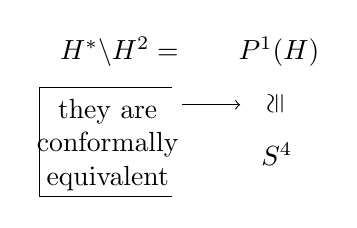
\begin{tikzpicture}[x=.93cm,y=.75cm,baseline]
\node at (.18,.06) {\(\mathbb H^*\backslash\mathbb H^2=\)};
\node at (2.36,.06) {\(\mathbb P^1(\mathbb H)\)};
\node[rotate=90] at (2.33,-.83) {\(\cong\)};
\node at (2.33,-1.67) {\(S^4\)};
\node[align=center] at (.02,-1.52) {they are\\conformally\\equivalent};
\draw (-.91,-.54)--(.90,-.54) (-.91,-.54)--(-.91,-2.40)--(.9,-2.40);
\draw[->] (1.04,-.84)--(1.83,-.84);
\end{tikzpicture}}\endgroup\par
--- the quaternionic projective line (left)\par
(\(\mathbb H\) --- the division ring of quaternions).}
\end{GelfandAdjacentEvidence}
\begin{GelfandAdjacentEvidence}{GELFAND-P000706}{3}


\(\mathbb C\subset\mathbb H\), hence a surj.
\(\mathbb C^*\backslash\mathbb H^2=\mathbb C P^3\)
and we have a map \(\mathbb C P^3\to S^4\) (its fibres are two-dimensional).

Conf. structure on \(\mathbb P^1(\mathbb H)\) --- with a point removed, it is
\(\mathbb R^4\cong\mathbb H\) with the standard conf. structure.
\Unclear{GELFAND-P000706}{hopf-conformal-exponent}{The superscript before the parenthesis is read as \(1\), as in the formula above the diagram. The lower stroke approaches the parenthesis.}
\end{GelfandAdjacentEvidence}
\begin{GelfandAdjacentEvidence}{GELFAND-P000706}{4}


Conf. structure: at \(\forall\) points a metric is given up to a positive multiplier.
The fibres of \(\mathbb C P^3\to S^4\) are \(\mathbb C P^1\).

Atiyah’s thm. establishes an isomorphism between

1) pairs \(\xi,\nabla\), satisfying the eqs. of duality

2) alg. vect. bundles on \(\mathbb C P^3\), trivial on each fibre of the map
\(\mathbb C P^3\overset{f}{\to}S^4\).

\uwave{Establishing the isomorphism}:

All lines (proj. complex) in \(\mathbb C P^3\) form a quadric, the fibres of the map \(f\) --- the real points of this quadric.
In \(\mathbb C P^3\) there is an involution \((z_1,z_2,z_3,z_4)\);
\[
\overset{\text{form a quaternion}}{(z_1+z_2j,\ z_3+z_4j)}
\]
\Unclear{GELFAND-P000706}{quaternion-annotation}{The circled note above the pair tentatively reads “сост. кватернион” (form a quaternion).}
\end{GelfandAdjacentEvidence}
\begin{GelfandAdjacentEvidence}{GELFAND-P000706}{5}

\Unclear{GELFAND-P000706}{first-quaternion-index}{The first index in the pair is read as \(1\). The slanting stroke and broad foot also allow \(2\).}
\end{GelfandAdjacentEvidence}


Multiply on the left by \(j\):
\[
\bar z_1j-\bar z_2,\qquad \bar z_3j-\bar z_4
\]


\Needspace{7\baselineskip}
\begin{GelfandAdjacentEvidence}{GELFAND-P000707}{1}
\SourcePage{GELFAND-P000707}{unlabelled}

Involution:
\[
(z_1,z_2,z_3,z_4)\mapsto(-\bar z_2,\bar z_1,-\bar z_4,\bar z_3)
\]
\uwave{Take the complex lines invariant under this involution}.
This gives \(S^4\).

Triviality is understood in the alg. (\(\sim\) complex) sense.

The bundles are pulled back from \(S^4\), but on \(S^4\) there is no complex structure.

\uwave{\(1)\Rightarrow 2)\)}
\[
\xi\mapsto f^*\xi
\]
Details next time.

\underline{I. Krichever.}\qquad \uwave{On constructing exact solutions of other nonlinear equations}.

\begin{equation}
\left[\frac{\partial}{\partial y}-L_1,\frac{\partial}{\partial t}-L_2\right]=0
\tag{1}
\end{equation}
\begin{equation}
L_1=\sum_{i=0}^n u_i(x,y,t)\frac{d^i}{dx^i}
\tag{2}
\end{equation}
\Incomplete{GELFAND-P000707}{right-margin-upper-marks}{Two vertical strokes with transverse traces are visible in the right margin beside (2).}
\end{GelfandAdjacentEvidence}
\begin{GelfandAdjacentEvidence}{GELFAND-P000707}{2}

\begin{equation}
L_2=\sum_{j=0}^m v_j(x,y,t)\frac{d^j}{dx^j}
\tag{3}
\end{equation}

The coefficients may also be matrices.

There are solutions in general position.

Separatrix family --- multisoliton [crossed out] solutions, of the eq.
\[
u_t=6uu_x+u_{xxx}.
\]
\Incomplete{GELFAND-P000707}{cancelled-soliton-word}{A short passage between “multisoliton” and “solutions” is heavily crossed out.}
\end{GelfandAdjacentEvidence}
\begin{GelfandAdjacentEvidence}{GELFAND-P000707}{3}


There are parameters. They are almost always conditionally periodic.

For certain vals. of the parameter --- rational.

\underline{Manin}. Solutions of alg. type (without \(y\)) --- those that are common solutions of (1) and
\begin{equation}
[L_1,L_3]=0
\tag{4}
\end{equation}
\Incomplete{GELFAND-P000707}{right-margin-lower-mark}{An isolated T-shaped mark is visible to the right of (4).}
\end{GelfandAdjacentEvidence}
\begin{GelfandAdjacentEvidence}{GELFAND-P000707}{4}

(\(L_3\) --- aux. operator)

Solns. [crossed out] of alg. type --- such that
\(\exists L_3\notin\mathbb C[L_1,L_2]\), such that cond. is satisfied (4).
\Incomplete{GELFAND-P000707}{cancelled-algebraic-word}{A short passage between “Solns.” and “of alg. type” is crossed out.}
\end{GelfandAdjacentEvidence}
\begin{GelfandAdjacentEvidence}{GELFAND-P000707}{5}


\uwave{Degenerate solutions}: in the lin. space of lin. combinations of coeffs. of fractional powers, to each corresponds an alg. curve.

Its genus is constant almost everywhere. Degeneration --- where the genus changes.
The genus [crossed out \(\ne 0\)?] [boxed below the line: \fbox{equals \(0\)}]
where there are multisoliton solutions and something else.
\Unclear{GELFAND-P000707}{cancelled-genus-condition}{The crossed-out writing resembles \(\ne 0\). “Equals \(0\)” is enclosed below.}
\end{GelfandAdjacentEvidence}
\begin{GelfandAdjacentEvidence}{GELFAND-P000707}{6}


There is alg. dependence of \(L_1\) and \(L_2\) --- Jacobson’s thm. (193…
\Unclear{GELFAND-P000707}{jacobson-year-suffix}{Three low marks resembling an ellipsis follow “193,” with faint strokes at the right edge.}
\end{GelfandAdjacentEvidence}



\Needspace{7\baselineskip}
\begin{GelfandAdjacentEvidence}{GELFAND-P000708}{1}
\SourcePage{GELFAND-P000708}{41}

\uwave{Moser’s work:} [above the line: (\href{https://onlinelibrary.wiley.com/doi/10.1002/cpa.3160300106}{Mc-Kean and Airault})]
seek solns. rational in \(x\) of KdV.
In \(t\) one obt. ordinary eqs. that can be solved explicitly.

\SourceFigure{GELFAND-P000708}{arrow-rule}{%
\par\begingroup\color{black}\GelfandFitDiagram{\begin{tikzpicture}[x=1cm,baseline]
\draw[<-] (0,0)--(1,0);
\fill (1.30,0) circle (.035cm);
\draw (1.70,0)--(3.14,0);
\end{tikzpicture}}\endgroup}
\end{GelfandAdjacentEvidence}
\begin{GelfandAdjacentEvidence}{GELFAND-P000708}{2}


\uwave{The rationality cond. for} KdV \uwave{replaces} the 3rd \uwave{operator}.

Apparently the same holds for \(\forall\) of the Lax eqs.:
\SourceFigure{GELFAND-P000708}{lax-underbracket}{%
\par\begingroup\color{black}\GelfandFitDiagram{\begin{tikzpicture}[baseline=(equation.base)]
\node[inner sep=3pt] (equation) {\(\dfrac{\partial L}{\partial t}=[P,L]\)};
\draw ([yshift=1pt]equation.south west)--([yshift=-3pt]equation.south west)--
      ([yshift=-3pt]equation.south east)--([yshift=1pt]equation.south east);
\end{tikzpicture}}\endgroup}
\end{GelfandAdjacentEvidence}



\Needspace{7\baselineskip}
\begin{GelfandAdjacentEvidence}{GELFAND-P000709}{1}
\SourcePage{GELFAND-P000709}{unlabelled}

\underline{12/\(\overline{\underline{\mathrm{IX}}}\)-77 }\quad
\uwave{Gelfand Sem.}

\underline{G. Margulis.}

\(G\) --- a semisimple connected Lie group, for simplicity let its centre be trivial,
\(G\supset\Gamma\) --- a discrete subgroup, such that [crossed out]
\[
\nu(G/\Gamma)<+\infty
\qquad(\nu\text{ --- volume induced by Haar measure})
\]
\Incomplete{GELFAND-P000709}{cancelled-before-volume}{A short passage to the left of the formula is crossed out.}
\end{GelfandAdjacentEvidence}
\begin{GelfandAdjacentEvidence}{GELFAND-P000709}{2}

Such \(\Gamma\) are called \uwave{lattices}.

An algebraic group \(G\) --- a subgroup of \(GL(n,\mathbb C)\), that is an alg. variety in \(GL(n,\mathbb C)\).
\Unclear{GELFAND-P000709}{algebraic-variety-abbreviation}{The abbreviation after “alg.” tentatively reads “много-зием” (variety).}
\end{GelfandAdjacentEvidence}
\begin{GelfandAdjacentEvidence}{GELFAND-P000709}{3}


\uwave{\(k\)-group} --- a group def. over the field \(k\)
(given by eqs. with coeffs. in \(k\)). (here \(k\subset\mathbb C\) a subfield)
(Otherwise: it is called \(k\)-closed).

Let \(G\) --- \(\mathbb Q\)-group.

\(G(k)\) --- set of matrices with coeffs. in \(k\), \(\in\) our set.

One can take points over a subring of \(\mathbb C\)
\[
G(\mathbb R)\supset G(\mathbb Z)
\]
\(G(\mathbb Z)\) is a group if [crossed out: \(G(\mathbb R)\)]
\(G(\mathbb Z)\subset SL(n,\mathbb Z)\).
\Unclear{GELFAND-P000709}{integral-cancellation}{The crossed-out writing before \(G(\mathbb Z)\subset SL(n,\mathbb Z)\) resembles \(G(\mathbb R)\).}
\end{GelfandAdjacentEvidence}
\begin{GelfandAdjacentEvidence}{GELFAND-P000709}{4}


1) \(G(\mathbb Z)\) is called an arithm. \uwave{subgroup}.

2) \(\Lambda\subset G(\mathbb R)\)

if \(\Lambda\) is commensurable with \(G(\mathbb Z)\), then
\(\Lambda\) is also called arithmetic.

([above the line: \(\Lambda\)] commensurable [above the line: with \(G(\mathbb Z)\)]
\(\underset{\mathrm{def}}{\Longleftrightarrow}\)
\(\Lambda\cap G(\mathbb Z)\) has finite index in \(\Lambda\) and in \(G(\mathbb Z)\))
\Unclear{GELFAND-P000709}{commensurability-insertions}{\(\Lambda\) and “with \(G(\mathbb Z)\)” are inserted above the line. “def” stands under the double arrow.}
\end{GelfandAdjacentEvidence}
\begin{GelfandAdjacentEvidence}{GELFAND-P000709}{5}


[crossed out: Question]
\Unclear{GELFAND-P000709}{question-cancellation}{Several rules cross out a word that tentatively reads “Question.”}
\end{GelfandAdjacentEvidence}
\begin{GelfandAdjacentEvidence}{GELFAND-P000709}{6}


Let \(H\subset G\), \(H\) is called an \uwave{arithmetic subgroup},
if [above the line with a pointer: alg. \(\mathbb Q\)-group]
\[
\exists G\subset GL(n,\mathbb C)\quad\text{and}\quad
f:G(\mathbb R)\longrightarrow G,
\]
\Unclear{GELFAND-P000709}{rational-group-insertion}{“alg. \(\mathbb Q\)-group” is written above with a pointer toward the following \(G\).}
\end{GelfandAdjacentEvidence}
\begin{GelfandAdjacentEvidence}{GELFAND-P000709}{7}


such that

1) \(f\) is an epimorphism, \quad
2) \(\operatorname{Ker} f\) is compact.

3) [above the line with a pointer: (image)] [crossed out]
\(f(G(\mathbb Z))\) is commensurable with \(H\).
\Incomplete{GELFAND-P000709}{cancelled-before-image}{Writing before \(f(G(\mathbb Z))\) is crossed out with slanting strokes.}
\end{GelfandAdjacentEvidence}
\begin{GelfandAdjacentEvidence}{GELFAND-P000709}{8}

\Unclear{GELFAND-P000709}{image-insertion}{“Image” is inserted above the crossed-out writing.}
\end{GelfandAdjacentEvidence}



\Needspace{7\baselineskip}
\begin{GelfandAdjacentEvidence}{GELFAND-P000710}{1}
\SourcePage{GELFAND-P000710}{unlabelled}

\underline{\underline{Property}}: if \(H\) --- an arithm. subgroup, then \(\nu(G/H)<\infty\).

(\href{https://www.mathnet.ru/eng/mat302}{Borel–Harish-Chandra theorem}

\underline{Example}: \(SL(n,\mathbb R)\supset SL(n,\mathbb Z)\)
\[
\nu\bigl(SL(n,\mathbb R)/SL(n,\mathbb Z)\bigr)<+\infty
\]
(Minkowski) [crossed out: or Hermite?].
\Unclear{GELFAND-P000710}{cancelled-after-minkowski}{Two words after “Minkowski” are crossed out. They tentatively read “or Hermite.”}
\end{GelfandAdjacentEvidence}
\begin{GelfandAdjacentEvidence}{GELFAND-P000710}{2}


\uwave{Exercise}: do it for \uwave{\(n=2\)} --- this is equiv. to finding the area of a triangle in the Lobachevsky plane.
\SourceFigure{GELFAND-P000710}{hyperbolic-triangle}{%
\par\begingroup\color{black}\GelfandFitDiagram{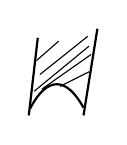
\begin{tikzpicture}[x=.88cm,y=.88cm,baseline]
\draw[thick] (0,0)--(.13,1.12) (.79,0)--(.99,1.25);
\draw[thick] (.02,.10) .. controls (.27,.58) and (.55,.55) .. (.79,.11);
\draw (.11,.79)--(.43,1.07);
\draw (.16,.59)--(.85,1.14);
\draw (.08,.35)--(.87,1.00);
\draw (.19,.38)--(.90,.88);
\draw (.45,.42)--(.87,.63);
\end{tikzpicture}}\endgroup}
\end{GelfandAdjacentEvidence}
\begin{GelfandAdjacentEvidence}{GELFAND-P000710}{3}


\underline{Theorem}: under certain additional conds. the converse holds, i.e.,
every lattice \uwave{is arithmetic}.
\uwave{Proof} is in the appendix to the book by \uwave{Raghunathan}.

For \(SL(2,\mathbb R)\) \uwave{it is false} --- there are parameters for tiling the Lobachevsky plane, and only countably many arithm. subgroups.

\underline{Selberg’s conjecture}: it is true for the remaining groups
Siegel also worked on this.

\[
G=\prod G_i,\qquad G_i\text{ --- simple Lie groups}
\]
\uwave{A latt.} \(\Gamma\) is called \uwave{reducible}, if
\(G=G_1\times G_2\), \(\dim G_i>0\),
and \((G_1\cap\Gamma)\times(G_2\cap\Gamma)\) has finite index in \(\Gamma\).

We study \uwave{irreducible lattices}.

\uwave{Conjecture}: for an irred. subgroup in \(G\ne SL(2,\mathbb R)/\{\pm E\}\)
[crossed out: this?] \(\forall\) lattice is arithmetic.
\Unclear{GELFAND-P000710}{cancelled-before-universal}{The crossed-out word before \(\forall\) tentatively reads “это” (this).}
\end{GelfandAdjacentEvidence}
\begin{GelfandAdjacentEvidence}{GELFAND-P000710}{4}


\uwave{Makarov, Vinberg}: found nonarithm. subgrps. in groups of motions of Lobachevsky spaces
\(SO(3,1)\), \(SO(4,1)\), \(SO(5,1)\)).

\underline{Answer}: if
\[
\underline{\underline{\operatorname{rank}G\ge 2}},\quad\text{then the theorem holds.}
\]
There is a parameter only in \(SL(2,\mathbb R)\).
In the remaining cases \uwave{rigidity}. (Selberg, A. Weil)

\uwave{In the other groups of rank 1 it is unknown}.

\uwave{Corollary of the rigidity thm.} (Selberg): \(\forall\) lattice
[crossed out] in \(SL(n,\) [crossed out] \(\mathbb R)\) is conjugate to a lattice with algebraic coefficients.
\Incomplete{GELFAND-P000710}{cancelled-after-lattice}{A short passage after “lattice” is heavily crossed out.}
\end{GelfandAdjacentEvidence}
\begin{GelfandAdjacentEvidence}{GELFAND-P000710}{5}

\Incomplete{GELFAND-P000710}{cancelled-before-real-field}{An isolated sign is crossed out before \(\mathbb R\) in \(SL(n,\mathbb R)\).}
\end{GelfandAdjacentEvidence}



\Needspace{7\baselineskip}
\begin{GelfandAdjacentEvidence}{GELFAND-P000711}{1}
\SourcePage{GELFAND-P000711}{44}
\underline{Main lemma}.

Let \(G\) --- a semisimple Lie group,
[enclosed insertion above the line: \(\operatorname{rank}G\ge 2\)],
\(\Gamma\) --- [enclosed insertion above the line: an irreducible] lattice in \(G\),
[inserted between the lines: \(G\) has no compact factors],
\(k\) --- a local field of char. \(0\), i.e. \(\mathbb C\), \(\mathbb R\) or a finite extension of
\(\mathbb Q_p\), \(n\in\mathbb N\) and let there be given a homomorphism
\(T:\Gamma\longrightarrow GL(n,k)\). Suppose

1) \(\overline{T(\Gamma)}\) is connected and simple.
(Zariski closure)

2) \(T(\Gamma)\) is not rel. compact

Then

I. \(k=\mathbb C\) or \(\mathbb R\)
\(\Rightarrow\) \(T\) extends to a repr. of the group \(G\)

II. \(k=\mathbb Q_p\) \(\Rightarrow\) conditions 1) and 2) are incompatible

\underline{Deduction of the theorem from the lemma}.

\(G=G(\mathbb R)\), \(K\) --- a field of alg. numbers,
we may assume \(\Gamma\subset G(K)\)
(easily proved [inserted above the line: by Selberg’s thm.]).

Let
\(\gamma_1,\ldots,\gamma_i\) be generators.
\Unclear{GELFAND-P000711}{last-generator-subscript}{The last subscript is tentatively \(i\), possibly \(l\).}
\end{GelfandAdjacentEvidence}
\begin{GelfandAdjacentEvidence}{GELFAND-P000711}{2}

Consid. the denominators of the corresp. matrices and the prime factors occurring in their factorization \(p_1,\ldots,p_m\).
\Unclear{GELFAND-P000711}{last-prime-subscript}{The last subscript in the list of prime factors is overwritten. It tentatively reads \(m\).}
\end{GelfandAdjacentEvidence}
\begin{GelfandAdjacentEvidence}{GELFAND-P000711}{3}


It suff. to prove that the image of
\Incomplete{GELFAND-P000711}{cancelled-before-gamma}{A short passage before \(\Gamma\) is crossed out.}
\end{GelfandAdjacentEvidence}
\begin{GelfandAdjacentEvidence}{GELFAND-P000711}{4}

\(\Gamma\) in \(G(\mathbb Q_p)\) is relat. compact.
Then the denominators are bounded
\Incomplete{GELFAND-P000711}{cancelled-before-in-aggregate}{A word after “bounded” is crossed out.}
\end{GelfandAdjacentEvidence}

jointly (from the structure of the topology in \(\mathbb Q_p\)).

Compactness follows from assertion II of the lemma. \(\blacksquare\)


\Needspace{7\baselineskip}
\begin{GelfandAdjacentEvidence}{GELFAND-P000712}{1}
\SourcePage{GELFAND-P000712}{unlabelled}
\underline{19/\(\overline{\underline{\mathrm{IX}}}\)---77 }
\quad \uwave{Gelfand Sem..}

\uwave{V. Drinfeld.} Consid. \(S^4\) with the conformal structure induced by the standard metric.

\(\xi\) --- a smooth complex vector bundle over \(S^4\).

\Unclear{GELFAND-P000712}{preceding-physics-cancellation}{The crossed-out text before the bracket tentatively reads “Кир” (Kir).}
\end{GelfandAdjacentEvidence}
\begin{GelfandAdjacentEvidence}{GELFAND-P000712}{2}

[A physicist is present: Kirzhnits, David Abramovich].

\uwave{Duality equations.} \quad \(A_\mu\) --- a matrix-valued fn. of 4 vars.,
\begin{equation*}
F_{\mu\nu}=\partial_\mu A_\nu-\partial_\nu A_\mu+[A_\mu,A_\nu],
\qquad \mu=1,2,3,4.\tag{1}
\end{equation*}
\Unclear{GELFAND-P000712}{cancelled-before-duality}{The crossed-out expression before equation (2) tentatively reads \(F_{ijk}\).}
\end{GelfandAdjacentEvidence}

\begin{equation*}
F_{ij}=\frac{1}{2}\varepsilon_{ijk\ell}F_{k\ell}
\qquad (\text{eqns.}\,\text{\uwave{of duality}})\tag{2}
\end{equation*}
\begin{equation*}
[\partial_\mu+A_\mu,F_{\mu\nu}]=0
\qquad (\text{eqns.}\,\text{\uwave{of Yang–Mills}})\tag{3}
\end{equation*}


\Needspace{7\baselineskip}
\begin{GelfandAdjacentEvidence}{GELFAND-P000713}{1}
\SourcePage{GELFAND-P000713}{unlabelled}
\underline{Kirzhnits} \uwave{David Abramovich} (from FIAN).

\uwave{On certain characteristic ideas of theor. physics.}

\Unclear{GELFAND-P000713}{front-mark}{The isolated mark before “Frontier” tentatively reads “4.”}
\end{GelfandAdjacentEvidence}
\begin{GelfandAdjacentEvidence}{GELFAND-P000713}{2}

Frontier: 1) elem. particles 2) cosmology 3) transition from dyn. systems to statist.

All this is now closely connected!

\Incomplete{GELFAND-P000713}{theory-mark}{A heavily overwritten or crossed-out mark precedes the heading.}
\end{GelfandAdjacentEvidence}
\begin{GelfandAdjacentEvidence}{GELFAND-P000713}{3}

\uwave{Theory of elementary particles.}

Arose \(\approx 50\) years ago.

For the first 20 years QFT ideas predominated, i.e. as in quant. mechanics.

\uwave{Late 1950s}: doubts.

\uwave{Landau}: “The Hamilton. method is a corpse. Our task is to bury it with all the honors due to it!”

1960s --- group approach.

Now a \uwave{renaissance} of the field approach. The idea responsible:

1. \uwave{Spontaneously broken symmetry.}

Sensitivity to macroscopic effects (symmetry breaking).

2. \uwave{Macroscopic effects.}

3. \uwave{History of the universe} --- an example of
\(\overbrace{\text{breaking}}^{\text{of such an influence}}\)
of spont. symm.

\uwave{Cosmology}

The universe is hot. Why?

4. “Dynamics --- statistics”.

\uwave{First, on pt. 4.} A few years ago something fundamentally new was said:
\uwave{Hawking, Bekenstein}

a region in phase space spreads out (owing to instability)
\SourceFigure{GELFAND-P000713}{phase-diagram}{%
\par\begingroup\color{black}\GelfandFitDiagram{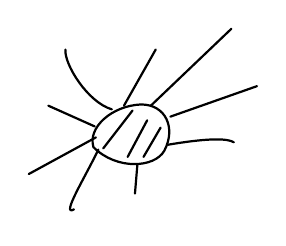
\begin{tikzpicture}[x=1.55cm,y=1.55cm,baseline,line cap=round]
\draw[thick] (-.32,-.12)
  .. controls (-.37,.04) and (-.17,.22) .. (.07,.23)
  .. controls (.27,.23) and (.36,.04) .. (.26,-.15)
  .. controls (.18,-.29) and (-.13,-.31) .. (-.32,-.12) -- cycle;
\draw[thick] (-.30,-.04)--(-.85,-.34)
  (-.28,-.14) .. controls (-.39,-.37) and (-.59,-.69) .. (-.48,-.63)
  (.04,-.26)--(.02,-.50)
  (.29,-.10) .. controls (.47,-.07) and (.75,-.03) .. (.83,-.08)
  (.31,.13)--(1.02,.38)
  (.15,.22)--(.81,.85)
  (-.07,.22)--(.19,.68)
  (-.17,.19) .. controls (-.37,.25) and (-.56,.56) .. (-.55,.68)
  (-.31,.05)--(-.69,.22);
\draw[thick] (-.24,-.13)--(.00,.18)
  (-.04,-.20)--(.12,.10)
  (.09,-.20)--(.23,.04);
\end{tikzpicture}}\endgroup}
\end{GelfandAdjacentEvidence}

--- was known. (e.g. Sinai’s billiard)

a syst. with positive entropy.

\uwave{The language of information} (Szilard, 1927, then mathematicians) worked here.

It spread out --- we lost information
\[
\Delta I=\underline{\text{Information}}=-\ln
\frac{P_f\;(\mathord{=}\text{ no. of poss. answers to the question at the end})}
{P_i\;(\mathord{=}\text{ --- ″ --- at the beginning})}
\]

\uwave{Entropy}

The macrostate is determ. by a small number of \uwave{parameters}. With these, different particle distributions are possible (degeneracy).

Entropy \(S=\ln(N_{\text{microscopic}})\)

\underline{I. M. G.}: Entropy: 27 coins, 1 counterf. lighter than the others --- 3 weighings.

\(N\) coins, 1 counterf. differs in weight. For what \(N\) can we find it in 3 weighings:

\underline{Solution}: \uwave{we know half as much} (\underline{\underline{13}}).

\(N\) weighings \((3^N-1)/2\).


\Needspace{7\baselineskip}
\begin{GelfandAdjacentEvidence}{GELFAND-P000714}{1}
\SourcePage{GELFAND-P000714}{47}
\underline{Algorithm.}

The coins must be divided so that the piles have equal entropy!!

(Divide the entropy into 3 equal parts).

No need for exhaustive search!

\begin{tabular}{@{}ll@{}}
coin & \(p\) --- prob. of heads \\
       & \(q\) --- prob. of tails
\end{tabular}
\[
S=p\ln p+q\ln q
\]
\Unclear{GELFAND-P000714}{binary-entropy-sign}{There is no visible minus sign before \(p\ln p\) in the manuscript.}
\end{GelfandAdjacentEvidence}
\begin{GelfandAdjacentEvidence}{GELFAND-P000714}{2}


Additivity makes it reasonable.

\uwave{\(N\) outcomes} \quad \(-\sum p_i\ln p_i\)
\qquad If \(p_i=\frac{1}{N}\), we get \(S=\ln N\)

\uwave{Inform.} \(=\) \uwave{change in entropy.}

\uwave{Soln. of problem}: look at the change in probabilities.

Start: \underline{\(4+4,5\)}
\[
\Delta I=-\ln\frac{N_f}{N_i}
\]

\uwave{K. D. A.}\quad \uwave{\(\Delta S=-\Delta I.\)}

\underline{Example}: gas
\SourceFigure{GELFAND-P000714}{gas-states}{%
\par\begingroup\color{black}\GelfandFitDiagram{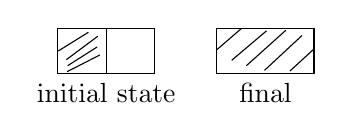
\begin{tikzpicture}[x=.85cm,y=.85cm,baseline]
\draw (0,0) rectangle (1.45,.68);
\draw (.73,0)--(.73,.68);
\draw (.01,.34)--(.46,.62) (.13,.21)--(.60,.56)
  (.15,.12)--(.59,.40) (.14,.03)--(.63,.28);
\node[below] at (.725,0) {initial state};
\draw (2.38,0) rectangle (3.83,.68);
\draw (2.38,.36)--(2.75,.68) (2.60,.20)--(3.12,.64)
  (2.82,.12)--(3.41,.65) (3.09,.05)--(3.65,.57)
  (3.47,.04)--(3.83,.37);
\node[below] at (3.105,0) {final};
\end{tikzpicture}}\endgroup}
\end{GelfandAdjacentEvidence}
\begin{GelfandAdjacentEvidence}{GELFAND-P000714}{3}

\[
S=\ln\frac{V}{N}\qquad(\text{per molecule}).
\]
\begin{center}
\begingroup\color{black}\GelfandFitDiagram{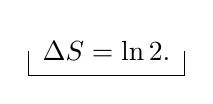
\begin{tikzpicture}
\node (delta) [inner sep=5pt] {\(\Delta S=\ln 2.\)};
\draw (delta.west)--(delta.south west)--(delta.south east)--(delta.east);
\end{tikzpicture}}\endgroup
\end{center}

Consequence: loss of inf. \(\Rightarrow\) increase in entropy

Gained inf. \(\Rightarrow\) decrease in inf.
\Unclear{GELFAND-P000714}{acquisition-consequence}{The start of “уменьш.” (decrease) is overwritten. The next abbrev. reads “инф.” (inf.).}
\end{GelfandAdjacentEvidence}
\begin{GelfandAdjacentEvidence}{GELFAND-P000714}{4}


Maxwell’s demon lowers entropy (keeps track of particles)

Are there any other ways of losing inf.?

Perhaps there are
\Incomplete{GELFAND-P000714}{forces-cancellation}{A word after “there are” is heavily crossed out.}
\end{GelfandAdjacentEvidence}
\begin{GelfandAdjacentEvidence}{GELFAND-P000714}{5}

forces retaining information
\Incomplete{GELFAND-P000714}{before-volume-cancellation}{An isolated mark before “in a g. volume” is crossed out.}
\end{GelfandAdjacentEvidence}

in a g. volume.

\uwave{A known situation where inform. is cut off by phys. means}

--- inf. does not get out.

There is such a force: \underline{gravitation}! (and it is the only one)

Long-range and of one sign (!)

“Black hole” --- a body that does not let information out.

Laplace thought of it: \uwave{Speed of light \(=2^{\underline{\text{nd}}}\) cosmic speed.}
\[
\frac{mv^2}{2}-\gamma\frac{mM}{R}=0
\]
\[
\frac{mc^2}{2}=\gamma\frac{mM}{R},
\]
\[
\boxed{R=\frac{2\gamma M}{c^2}=r_g}
\]

At this radius light will not leave the body (nor any signal)

--- it turns out to hold in exact science too


\Needspace{7\baselineskip}
\begin{GelfandAdjacentEvidence}{GELFAND-P000715}{1}
\SourcePage{GELFAND-P000715}{unlabelled}
\[
R_{\text{Sun}}=10^6\ \text{km}
\]
\Unclear{GELFAND-P000715}{mass-cancellation}{An isolated sign before “For” is heavily crossed out.}
\end{GelfandAdjacentEvidence}
\begin{GelfandAdjacentEvidence}{GELFAND-P000715}{2}

For its mass the required rad. is \underline{\underline{\(7\) km.}}

In principle we can know nothing about a black hole except a few params. ---
--- mass, charge,
\Incomplete{GELFAND-P000715}{charge-cancellation}{The entry after “charge” is heavily crossed out.}
\end{GelfandAdjacentEvidence}
\begin{GelfandAdjacentEvidence}{GELFAND-P000715}{3}

radius.

As with a gas. An enormous number of microstates.
In fact it is a \uwave{thermodyn. object}!!

\(\underset{\text{(earlier)}}{\text{\uwave{Hawking}}}\):
the black hole’s surf. \(S\) (!) increases in all processes.
Merger of 2 black holes. Geom. clearly increases (from Laplace’s formula)

The letter \(S\) played a remarkable role.
\[
\begingroup\color{black}\GelfandFitDiagram{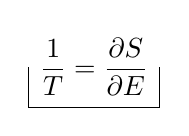
\begin{tikzpicture}[baseline=(definition.base)]
\node (definition) [inner sep=4pt] {\(\displaystyle \frac{1}{T}=\frac{\partial S}{\partial E}\)};
\draw (definition.west)--(definition.south west)--(definition.south east)--(definition.east);
\end{tikzpicture}}\endgroup
\quad\Rightarrow\quad T\text{ --- the black hole’s “temp.”.}
\]

\(\underset{\text{(Hawking’s pupil)}}{\text{\uwave{Bekenstein}}}\) ---
removed the quotation marks! Counted the information lost in forming black holes!!
Agrees with informational entropy.

Let us throw a hot body into a black hole. It increases the surf. more than a cold one, in exact corresp. with the entropy increase.

[crossed out: Hawking.] \underline{\underline{Hawking}}.
Merger of pairs of particles. The black hole radiates and its spectrum is Planckian!
\[
\frac{1}{e^{\frac{\hbar\omega}{kT}}-1}
\]
\(T\) --- that temperature.

Inf. is lost not by stochasticization!!, but goes into black holes.
(mechanically cut off)

Other ways

\uwave{\href{https://doi.org/10.1103/PhysRevD.14.870}{Uhnru?}}
\Unclear{GELFAND-P000715}{unruh-name}{The spelling tentatively reads “Uhnru.” The passage refers to \href{https://doi.org/10.1103/PhysRevD.14.870}{W. G. Unruh}.}
\end{GelfandAdjacentEvidence}
\begin{GelfandAdjacentEvidence}{GELFAND-P000715}{4}

Homog. gravitational field.

Let a particle move with uniform acceleration in vacuum.
Light from some places will not reach it.

\SourceFigure{GELFAND-P000715}{unruh-diagram}{%
\par\begingroup\color{black}\GelfandFitDiagram{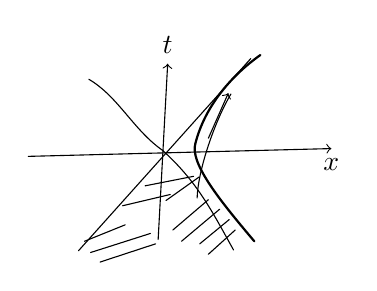
\begin{tikzpicture}[x=1.1cm,y=1.1cm,baseline,line cap=round]
\draw[->] (-1.55,-.07)--(1.95,.02) node[below] {\(x\)};
\draw[->] (-.05,-1.03)--(.06,1.0) node[above] {\(t\)};
\draw (-.97,-1.16)--(1.02,1.06);
\draw (-.85,.82) .. controls (-.51,.62) and (-.34,.24) .. (0,0)
  .. controls (.40,-.36) and (.57,-.70) .. (.82,-1.15);
\draw[thick] (1.06,-1.05) .. controls (.68,-.60) and (.31,-.15) .. (.38,.08)
  .. controls (.48,.47) and (.75,.83) .. (1.13,1.10);
\draw (.40,-.55) .. controls (.41,-.23) and (.60,.33) .. (.79,.65);
\draw[->] (.53,.14)--(.76,.66);
\draw (-.83,-1.18)--(-.14,-.96) (-.72,-1.29)--(-.08,-1.08)
  (-.90,-1.05)--(-.43,-.86) (-.46,-.64)--(.09,-.51)
  (-.20,-.41)--(.36,-.30) (.04,-.58)--(.42,-.31)
  (.12,-.92)--(.53,-.57) (.22,-1.05)--(.66,-.68)
  (.43,-1.08)--(.77,-.80) (.53,-1.20)--(.84,-.92);
\end{tikzpicture}}\endgroup\par\smallskip
The exact joins of the overlapping strokes and curves at right are indeterminate.}
\end{GelfandAdjacentEvidence}
\begin{GelfandAdjacentEvidence}{GELFAND-P000715}{5}


It turns out that light reaches it only from \uwave{half of space}.
The obs. will see (calculation) a \uwave{Planck distribution}.
The zero-point oscillations look distorted to him.
This is a difficult calculation.

\(H\) --- Ham. of the electromagn. field.
\[
H\lvert\Phi\rangle=E_0\lvert\varphi\rangle
\]
\Unclear{GELFAND-P000715}{hamiltonian-state}{The state sign at left is heavily retraced and looks like \(\Phi\). At right it looks like \(\varphi\).}
\end{GelfandAdjacentEvidence}
\begin{GelfandAdjacentEvidence}{GELFAND-P000715}{6}


The state vector from the point of view of a non-inert. obs. \(\rightarrow\) Calc. prob. of
\(1^{\underline{\text{st}}}\), \(2^{\underline{\text{nd}}}\) and more

\Unclear{GELFAND-P000715}{outer-right-fragments}{Two clipped groups of strokes are visible beyond the right page border.}
\end{GelfandAdjacentEvidence}



\Needspace{7\baselineskip}
\begin{GelfandAdjacentEvidence}{GELFAND-P000716}{1}
\SourcePage{GELFAND-P000716}{48?}
\Unclear{GELFAND-P000716}{folio}{The last digit of the folio number tentatively reads 8, possibly 2.}
\end{GelfandAdjacentEvidence}
\begin{GelfandAdjacentEvidence}{GELFAND-P000716}{2}

photons.
\[
\begingroup\color{black}\GelfandFitDiagram{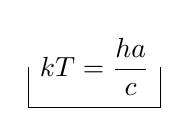
\begin{tikzpicture}[baseline=(temp.base)]
\node (temp) [inner sep=4pt] {\(\displaystyle kT=\frac{ha}{c}\)};
\draw (temp.west)--(temp.south west)--(temp.south east)--(temp.east);
\end{tikzpicture}}\endgroup\quad\Rightarrow\quad\text{temperature}
\]
\Unclear{GELFAND-P000716}{temperature-constant}{The first sign in the numerator reads \(h\). A distinct bar for \(\hbar\) is indiscernible.}
\end{GelfandAdjacentEvidence}
\begin{GelfandAdjacentEvidence}{GELFAND-P000716}{3}


Heating of the gas at the finish.

\uwave{Why is the universe hot?}

[At left] Experiment --- it is cooling now \(\Vert\)

[At right] \underline{\underline{\(T=3^{\circ}\mathrm K\)}} --- from the distrib. of
\Incomplete{GELFAND-P000716}{temperature-cancellation}{A word before “Planck” is heavily crossed out.}
\end{GelfandAdjacentEvidence}
\begin{GelfandAdjacentEvidence}{GELFAND-P000716}{4}

Planck for rad. from space.
[below the formula: (relic radiation)]

There was a region of the unknown.
It arose at some point in time. Before this it makes no sense [below: to ask].

\uwave{There is an event horizon}.
\SourceFigure{GELFAND-P000716}{horizon-drawing}{%
\par\begingroup\color{black}\GelfandFitDiagram{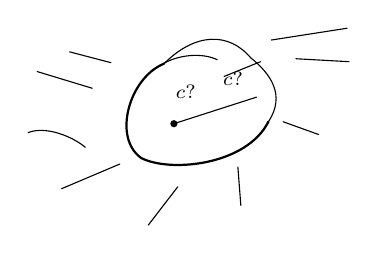
\begin{tikzpicture}[x=1.25cm,y=1.25cm,baseline,line cap=round]
\draw[thick] (-.30,.46) .. controls (-.65,.32) and (-.83,-.29) .. (-.53,-.50)
  .. controls (-.23,-.65) and (.54,-.57) .. (.76,-.13);
\draw (.76,-.13) .. controls (.94,.14) and (.78,.36) .. (.58,.52)
  .. controls (.36,.78) and (.02,.78) .. (-.30,.46);
\draw (-.31,.46) .. controls (-.11,.57) and (.12,.56) .. (.24,.50);
\draw (-1.26,.58)--(-.84,.47) (-1.59,.38)--(-1.03,.21)
  (-1.68,-.24) .. controls (-1.50,-.17) and (-1.23,-.28) .. (-1.10,-.39)
  (-1.34,-.81)--(-.75,-.56) (-.46,-1.18)--(-.16,-.79)
  (.48,-.98)--(.45,-.59) (.79,.70)--(1.56,.82)
  (1.04,.51)--(1.58,.48) (.91,-.13)--(1.27,-.26);
\fill (-.20,-.15) circle[radius=1.3pt];
\draw (-.20,-.15)--(.64,.12) (.31,.33)--(.68,.48);
\node at (-.08,.17) {\scriptsize\(c?\)};
\node at (.40,.31) {\scriptsize\(c?\)};
\end{tikzpicture}}\endgroup\par\smallskip
The ends of the interior strokes and the two small signs are only partly legible.}
\end{GelfandAdjacentEvidence}
\begin{GelfandAdjacentEvidence}{GELFAND-P000716}{5}

\underline{closed region} (light has had no time to arrive from there).
(\(\Rightarrow\) hence this temp. for us.)

\begin{center}
\rule[.45ex]{1.4em}{.35pt}\,\(\cdot\)\,\rule[.45ex]{1.4em}{.35pt}
\end{center}
Spontaneous symm. breaking.
\SourceFigure{GELFAND-P000716}{symmetry-curves}{%
\par\begingroup\color{black}\GelfandFitDiagram{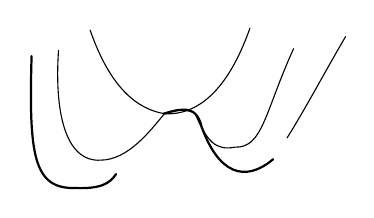
\begin{tikzpicture}[x=1.18cm,y=1.18cm,baseline,line cap=round]
\draw (-.84,.90) .. controls (-.62,.27) and (-.33,.05) .. (-.04,0)
  .. controls (.31,-.02) and (.64,.24) .. (.88,.92);
\draw (-1.18,.68) .. controls (-1.23,-.07) and (-1.07,-.52) .. (-.73,-.50)
  .. controls (-.43,-.50) and (-.19,-.18) .. (-.04,0)
  .. controls (.04,.05) and (.22,.06) .. (.29,.00)
  .. controls (.42,-.30) and (.51,-.40) .. (.72,-.36)
  .. controls (1.02,-.37) and (1.04,.02) .. (1.35,.70);
\draw[thick] (-1.47,.62) .. controls (-1.50,-.45) and (-1.45,-.81) .. (-1.00,-.80)
  .. controls (-.72,-.81) and (-.63,-.75) .. (-.56,-.65);
\draw[thick] (-.05,0) .. controls (.11,.04) and (.30,.12) .. (.36,-.14)
  .. controls (.54,-.64) and (.82,-.75) .. (1.13,-.49);
\draw (1.28,-.26) .. controls (1.47,.04) and (1.72,.51) .. (1.91,.83);
\end{tikzpicture}}\endgroup\par\smallskip
The precise joins where the lines overlap are indeterminate.}
\end{GelfandAdjacentEvidence}
\begin{GelfandAdjacentEvidence}{GELFAND-P000716}{6}

\uwave{evolution of the well upon a disruption of temperature}
\Unclear{GELFAND-P000716}{minimum-temperature}{The caption tentatively reads “evolution of the well upon a disruption of temperature.” “Minima” is also possible for “well.”}
\end{GelfandAdjacentEvidence}


\begin{center}
\rule[.45ex]{2.1em}{.45pt}\,\(\cdot\)\,\rule[.45ex]{2.1em}{.45pt}
\end{center}
An idea of \uwave{Senya Vishik}, on why the Gelfand sem. is unsterilized:
“To integrate successfully over a large domain one must use the Monte Carlo method.”


\Needspace{7\baselineskip}
\begin{GelfandAdjacentEvidence}{GELFAND-P000717}{1}
\SourcePage{GELFAND-P000717}{55}
\underline{3/\(\overline{\underline{\mathrm X}}\)---77}
\qquad \underline{Gelfand Sem..}

\begin{flushright}
To be treated systematically: “noncommutative algebraic geometry”
\end{flushright}

\underline{\underline{L. A. Dikii.}}\qquad \underline{On new Lie algebras.}

(\uwave{Gelf., Dikii}, \href{https://www.mathnet.ru/eng/faa2064}{Funct. Anal., 11:2}).

Def. 1. \quad \uwave{The algebra \(A\).}

\Unclear{GELFAND-P000717}{cancelled-top}{The crossed-out text at right begins “В” (In), followed by a word tentatively read as “себе.”}
\end{GelfandAdjacentEvidence}
\par\begingroup\setlength{\parindent}{0pt}\setlength{\parskip}{.4em}\raggedright


\[
u_k^{(i)},\qquad k=0,1,\ldots,n;\qquad i=0,1,2,\ldots
\]
\[
A=\left\{\sum a\,u_{k_1}^{(i_1)}u_{k_2}^{(i_2)}u_{k_3}^{(i_3)}
\cdots u_{k_N}^{(i_N)}\right\},\qquad a\in\underset{\text{(field)}}{K},
\]
\begin{flushright}
\(A\) --- the alg. of polynomials\\
in the generators \(u_k^{(i)}\)\\
\fbox{\(A=K[u_k^{(i)}].\)}
\end{flushright}
\[
\xi=\sum a_{k,i}\frac{\partial}{\partial u_k^{(i)}},\qquad a_{k,i}\in A.
\]
(the sum is infinite)\qquad \(\xi\) is called a derivation
\[
\frac{d}{dx}=\sum_{k,i}u_k^{(i+1)}\frac{\partial}{\partial u_k^{(i)}}
\]
\[
\frac{d}{dx}u_k^{(i)}=u_k^{(i+1)};\qquad
u_k^{(i)}=\left(\frac{d}{dx}\right)^i u_k;\qquad
u_k\underset{\mathrm{def}}{=}u_k^{(0)}
\]

\underline{Def.} 2. \quad \uwave{The space} \(\widetilde A\) (space of functionals)

From now on, always \(u_n=1\), \(u_{n-1}=0\).
\[
\left\{f:\ \exists g,\ f=\frac{d}{dx}g\right\}=\frac{d}{dx}A;
\]
\[
\widetilde A=A\big/\frac{d}{dx}A
\]
\[
f\longmapsto f\bmod\frac{d}{dx}A=\widetilde f\in\widetilde A
\]
\[
A\underset{\int\cdots\,dx}{\longrightarrow}\widetilde A
\qquad\qquad
\widetilde f=\int f\,dx
\]

\underline{Problem.}
\[
f[u]\in\mathbb C[u_k^{(i)}];
\]
\[
\int_{-\infty}^{\infty}f[u(x)]\,dx=0,\quad\forall u\in S(\mathbb R^1)
\quad\Longleftrightarrow\quad
f\in\frac{d}{dx}\mathbb C[u].
\]

\par\endgroup
\begin{GelfandAdjacentEvidence}{GELFAND-P000717}{2}
\underline{Def. 3}. \quad
\(A^{n-1}={}\) space of tuples \((f_0,f_1,\ldots,f_{n-2})\), \(f_k\in A\)

[in the left margin: \(\frac{\delta}{\delta u}\).]
\[
\frac{\delta}{\delta u}:\widetilde A\longrightarrow A^{n-1}
\]
\[
\left(\frac{\delta\widetilde f}{\delta u}\right)_k
=\sum_{\ell=0}^{\infty}\left(-\frac{d}{dx}\right)^\ell
\frac{\partial f}{\partial u_k^{(\ell)}}
=\frac{\delta\widetilde f}{\delta u_k}
\]
\Unclear{GELFAND-P000717}{variational-numerator}{The \(f\) in the numerator under the sum is heavily retraced.}
\end{GelfandAdjacentEvidence}

(here \(\widetilde f=f\bmod\frac{d}{dx}A\))


\Needspace{7\baselineskip}
\begin{GelfandAdjacentEvidence}{GELFAND-P000718}{1}
\SourcePage{GELFAND-P000718}{unlabelled}
\underline{Def. 4.}\quad \(\ell:A^{n-1}\longrightarrow A^{n-1}\)
\[
f=(f_0,\ldots,f_{n-2})
\]
\[
(\ell f)_r=\sum_s\ell_{rs}f_s
\]
\[
\begin{aligned}
\ell_{rs}&=\sum_{\gamma=0}^{n-1-r-s}
\Biggl[\binom{\gamma+r}{r}u_{r+s+\gamma+1}
\left(-i\frac{d}{dx}\right)^\gamma-\\
&\qquad-\binom{\gamma+s}{s}\left(i\frac{d}{dx}\right)^\gamma
u_{r+s+\gamma+1}\Biggr]
\end{aligned}
\]
\Unclear{GELFAND-P000718}{operator-line-break}{The manuscript repeats the minus at the line break, at the end of the first line and at the start of the second.}
\end{GelfandAdjacentEvidence}
\par\begingroup\setlength{\parindent}{0pt}\setlength{\parskip}{.4em}\raggedright


\underline{\(n=2,3\)} easy;\qquad \underline{\(n=4\)} --- 1st substantial example.

\underline{Def. 5.}\quad \(\forall f\in A^{n-1}\) we construct
\[
\partial_f=\sum_{k,\ell}f_k^{(\ell)}\frac{\partial}{\partial u_k^{(\ell)}}
\qquad\text{(a derivation)}
\]
It is easy to check that
\[
\partial_f\frac{d}{dx}=\frac{d}{dx}\partial_f
\]
The operation is therefore defined \(\partial_f:\widetilde A\longrightarrow\widetilde A\).

\underline{Def. 6.}\quad Let \(f,g\in A^{n-1}\). Put
\[
([f,g])_r=\partial_f g_r-\partial_g f_r
\]
It is easy to check that
\[
[\partial_f,\partial_g]=\partial_{[f,g]}.
\]
Hence the commutator \([\cdot,\cdot]\) defines on \(A^{n-1}\) the structure of a Lie algebra.

\underline{Def. 7.}\quad def. of the commutator in \(\widetilde A\).
\[
\{\widetilde f,\widetilde g\}
=\int\sum_{r,s}\frac{\delta\widetilde f}{\delta u_r}\cdot
\ell_{rs}\frac{\delta\widetilde g}{\delta u_s}\,dx
\]

\par\endgroup
\begin{GelfandAdjacentEvidence}{GELFAND-P000718}{2}
\underline{Theorem:}
\Incomplete{GELFAND-P000718}{theorem-cancellation}{A word after “Theorem” is heavily crossed out.}
\end{GelfandAdjacentEvidence}
\begin{GelfandAdjacentEvidence}{GELFAND-P000718}{3}

we get a Lie algebra
\Unclear{GELFAND-P000718}{theorem-verb}{The verb tentatively reads “получается” (we get), possibly “получится” (we will get).}
\end{GelfandAdjacentEvidence}

(i.e. the Jacobi identity is satisfied)

\underline{Problem:} prove it more simply.

\underline{S. P. Novikov}\qquad
\(A=\frac{d^3}{dx^3}+\left(u\frac{d}{dx}+\frac{d}{dx}u\right)\)

also defines a Lie algebra.

(and the KdV eq. can be written with its help).


\Needspace{7\baselineskip}
\begin{GelfandAdjacentEvidence}{GELFAND-P000719}{1}
\SourcePage{GELFAND-P000719}{56}
\underline{S. I. Gelfand.} on the work of I. M. Gelf., I. N. Bernsh. and his own?:
\Unclear{GELFAND-P000719}{heading-final-word}{The last word tentatively reads “свои.” (his own). The final strokes run together.}
\end{GelfandAdjacentEvidence}
\begin{GelfandAdjacentEvidence}{GELFAND-P000719}{2}


\begin{flushright}
\fbox{\parbox{.66\linewidth}{“The local structure of the category of Harish–Chandra modules”\\or “Noncommutative algebraic geometry I”.}}
\end{flushright}

\(G\) --- a real Lie group, semisimple

\(K\subset G\), \(K\) --- a maximal compact subgroup

\(\mathfrak g\) --- the Lie algebra of the group \(G\)

\underline{Definition.} A Harish–Chandra module \(M\) ---
is a linear space over \(\mathbb C\) with actions of \(\mathfrak g\) and \(K\) and with conditions
(besides the natural conds. for the actions and compatibility of the actions of \(\mathfrak g\) and \(K\)).

1) the actions of [crossed out: the Lie algebra of the group \(K\)] \(\mathfrak g\) and \(K\) are compatible:

a) the Lie alg. of \(K\) acts on \(M\) as a subalgebra in \(\mathfrak g\).

b) [crossed out: a)?]
\Unclear{GELFAND-P000719}{canceled-condition-label}{A sign after “б)” is crossed out. It tentatively reads “а)”.}
\end{GelfandAdjacentEvidence}
\begin{GelfandAdjacentEvidence}{GELFAND-P000719}{3}

\[
T\bigl(\underset{\substack{\uparrow\\K}}{k}\,
\underset{\substack{\uparrow\\\mathfrak g}}{X}\,k^{-1}\bigr)
=T_1(k)T(X)T_1(k^{-1}).
\]
\(T\) --- the action of \(\mathfrak g\), \(T_1\) --- the action of \(K\)

2) \(M\) decomposes with respect to \(K\) into a direct sum of [inserted above: irred.]
representations and each [inserted below: irred.] repr. occurs a finite number of times.

H.–C. mods. form a \uwave{category}. Morphisms are defined in the natural way.

\uwave{Problem}: description of this category.

\uwave{Idea}: there is a noncommut. algebra responsible for this.

\uwave{\href{https://www.mathnet.ru/eng/rm5609}{Gelfand, Ponomarev}}:
for the Lorentz group [inserted below: \(SL(2,\mathbb C)\)] it reduces to classifying pairs of matrices
\(A,B\), such that \(AB=BA=0\),
[crossed out: and]
\Incomplete{GELFAND-P000719}{canceled-matrices}{Two more words after “and” are crossed out.}
\end{GelfandAdjacentEvidence}
\begin{GelfandAdjacentEvidence}{GELFAND-P000719}{4}


\(U(\mathfrak g)\) --- the enveloping alg. of \(\mathfrak g\)

\(Z(\mathfrak g)\) --- its centre

\[
M\rightsquigarrow J_M=\{z\in Z(\mathfrak g)\mid zM=0\}
\qquad\text{(an ideal) in }Z(\mathfrak g).
\]

\(\Theta\) --- the set of characters \(\theta:Z(\mathfrak g)\to\mathbb C\).
(homomorphisms)

[crossed out beneath the formula: (linear formulas?)] \((\subset\mathbb C^N)\).
\Unclear{GELFAND-P000719}{canceled-theta-abbrev}{The crossed-out abbreviation after “linear” tentatively reads “ф-лы” (formulas).}
\end{GelfandAdjacentEvidence}
\begin{GelfandAdjacentEvidence}{GELFAND-P000719}{5}

\Unclear{GELFAND-P000719}{theta-ambient-exponent}{The case of the exponent in \(\mathbb C^N\) is unclear, \(N\) or \(n\).}
\end{GelfandAdjacentEvidence}


\begin{gather*}
\operatorname{supp}M\subset\Theta\\
\operatorname{supp}M=\{\theta\mid J_M\subset\ker\theta\}
\end{gather*}
\(\operatorname{supp}M\) --- a finite set.

Let \(D\subset\Theta\),
\[
C_D=\{M\mid\operatorname{supp}M\subset D\}.
\]


\Needspace{7\baselineskip}
\begin{GelfandAdjacentEvidence}{GELFAND-P000720}{1}
\SourcePage{GELFAND-P000720}{unlabelled}
We can consid. H.–C. modules with supp. at a point \(C_{\{\theta\}}\)

\underline{Theorem} (easy).
\[
C_D=\bigoplus_{\theta\in D}C_{\{\theta\}}
\]
\Incomplete{GELFAND-P000720}{canceled-sum-symbol}{A mark between the equals sign and \(\bigoplus\) is crossed out.}
\end{GelfandAdjacentEvidence}
\begin{GelfandAdjacentEvidence}{GELFAND-P000720}{2}

in a certain sense,

(they decompose and there are no homomorphisms).

\underline{1st main theorem.} Let \(D\) --- a bounded domain in \(\Theta\)
(in the complex sense). Then \(\exists\ Z(\mathfrak g)\)-algebra \(Q\)
\Unclear{GELFAND-P000720}{algebra-canceled-sign}{A small mark at the lower right of \(Q\) is crossed out. It may be a subscript.}
\end{GelfandAdjacentEvidence}
\begin{GelfandAdjacentEvidence}{GELFAND-P000720}{3}

[crossed out: such] with a finite number \(a\) of additive \(Z(\mathfrak g)\)-generators,
[inserted above: such that] [crossed out: Then?]
\(C_D\) is equivalent to the category of \(Q\)-modules that are finite-dimensional over \(\mathbb C\).
\Unclear{GELFAND-P000720}{canceled-theorem-word}{The crossed-out word before \(C_D\) tentatively reads “Тогда” (Then).}
\end{GelfandAdjacentEvidence}
\begin{GelfandAdjacentEvidence}{GELFAND-P000720}{4}


(\(\exists\) a functor realizing the equivalence)

\(Q\) --- \(Z(\mathfrak g)\)

\begin{center}--- \(\cdot\) ---\end{center}

\(\underset{23/\overline{\underline{\mathrm{IX}}}\text{-}77}{\text{“Izvestia”}}\)
and
\(\underset{22/\overline{\underline{\mathrm{IX}}}\text{-}77}{\text{“Socialist Industry”}}\)
[crossed out: dated the 23rd]

a report from Petrozavodsk of an unidentified flying object

\begin{center}--- \(\cdot\) ---\end{center}

\underline{Example.}
\begin{gather*}
G=SL_2(\mathbb R)/\{\pm1\}\\
Z(\mathfrak g)\cong\mathbb C[z]\\
\Theta=\mathbb C^1
\end{gather*}

\SourceFigure{GELFAND-P000720}{central-character-disk}{%
\par\begingroup\color{black}\GelfandFitDiagram{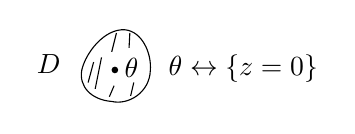
\begin{tikzpicture}[baseline]
\node at (-.87,.06) {\(D\)};
\draw (-.45,-.02) .. controls (-.40,.20) and (-.16,.51) .. (.10,.49)
  .. controls (.31,.47) and (.44,.20) .. (.42,-.03)
  .. controls (.41,-.30) and (.15,-.47) .. (-.07,-.42)
  .. controls (-.33,-.40) and (-.49,-.23) .. (-.45,-.02);
\draw (-.37,-.18)--(-.30,.08) (-.28,-.26)--(-.20,.14)
  (-.07,.21)--(-.01,.45) (.15,.26)--(.16,.45)
  (-.10,-.36)--(-.04,-.22) (.17,-.35)--(.21,-.18);
\fill (-.03,-.02) circle[radius=1.2pt];
\node at (.18,.00) {\(\theta\)};
\node at (1.60,.00) {\(\theta\leftrightarrow\{z=0\}\)};
\end{tikzpicture}}\endgroup}
\end{GelfandAdjacentEvidence}


We will construct the algebra over analytic fns.
\[
Q=(a_{ij}(z))_{i,j=1}^{3}\text{ --- matr. }3\times3,
\qquad a_{ij}(z)\text{ --- entire fns.}
\]
\[
(a_{ij}(0))=
\begin{pmatrix}
*&0&0\\
*&*&0\\
*&0&*
\end{pmatrix}
\]


\Needspace{7\baselineskip}
\begin{GelfandAdjacentEvidence}{GELFAND-P000721}{1}
\SourcePage{GELFAND-P000721}{unlabelled}
\underline{10/\(\overline{\underline{\mathrm X}}\)---77}
\qquad\underline{\underline{Gelfand Sem..}}

\underline{S. Gelfand.}

\(G\) --- a semisimple real Lie group

\(K\) --- a maximal compact subgroup

\(\mathfrak g\) --- the Lie algebra of the group \(G\)

\(U(\mathfrak g)\) --- the enveloping algebra.

\(Z(\mathfrak g)\) --- the centre of \(U(\mathfrak g)\)

Harish–Chandra module (HCM) \(V\), if

[\underline{H.–C. thm.:} in an irreduc. repr. of a semisimple group, every
[inserted above: irred.] repr. of the max. comp. group \(K\) occ. a finite no. of times]

In \(V\) there are given reprs. \(T_1\) of the alg. \(U(\mathfrak g)\), \(T_2\) --- a repr. of the group \(K\).

1) \(V\) --- a finitely gen. \(U(\mathfrak g)\)-module.

2) \(\left.T_1\right|_{\mathfrak k}=dT_2\),
\[
T_2(k)T_1(X)T_2(k^{-1})=T_1(kXk^{-1})
\]

3) \(T_2=\bigoplus\) irred. cont. reprs. of \(K\), and each occurs a finite number of times.

(direct sum in the literal sense).

\Incomplete{GELFAND-P000721}{canceled-result-heading}{A short passage before “Result” is heavily crossed out.}
\end{GelfandAdjacentEvidence}
\begin{GelfandAdjacentEvidence}{GELFAND-P000721}{2}

\underline{Result:} let
\[
\Theta=\{\theta:Z(\mathfrak g)\to\mathbb C\}=\mathbb C^{r}
\]
\Unclear{GELFAND-P000721}{theta-exponent}{The exponent tentatively reads \(r\), possibly \(\tau\).}
\end{GelfandAdjacentEvidence}
\begin{GelfandAdjacentEvidence}{GELFAND-P000721}{3}

(ring homomorphisms)

\[
V\mapsto\operatorname{supp}V\subset\Theta
\]
\[
\theta(z)\in\operatorname{supp}V
\Longleftrightarrow\exists\underset{\substack{\uparrow\\V}}{v}:
T_1(z)v=\theta(z)v,\quad z\in Z(\mathfrak g).
\]
\Unclear{GELFAND-P000721}{support-criterion}{The manuscript has \(\theta(z)\) on the left and gives no explicit condition \(v\ne0\).}
\end{GelfandAdjacentEvidence}
\begin{GelfandAdjacentEvidence}{GELFAND-P000721}{4}


In fact
\Incomplete{GELFAND-P000721}{canceled-support-symbol}{A short passage under the insertion “\(\operatorname{supp}V\) —” is heavily crossed out.}
\end{GelfandAdjacentEvidence}
\begin{GelfandAdjacentEvidence}{GELFAND-P000721}{5}

[inserted above: \(\operatorname{supp}V\) ---] a finite set.

Let there be a bounded domain \(D\subset\Theta\),
\[
C_D=\{V:\operatorname{supp}V\subset D\}.
\]
For disjoint sets \(D_1\) and \(D_2\) we get the direct sum of categories.

\uwave{Equivalence of categories:}
\SourceFigure{GELFAND-P000721}{category-equivalence}{%
\par\begingroup\color{black}\GelfandFitDiagram{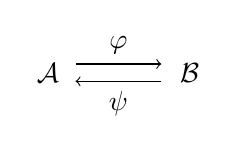
\begin{tikzpicture}[baseline]
\node (a) at (0,0) {\(\mathcal A\)};
\node (b) at (1.8,0) {\(\mathcal B\)};
\draw[->] (.35,.11)--(1.44,.11) node[midway,above] {\(\varphi\)};
\draw[->] (1.44,-.11)--(.35,-.11) node[midway,below] {\(\psi\)};
\end{tikzpicture}}\endgroup}
\end{GelfandAdjacentEvidence}
\begin{GelfandAdjacentEvidence}{GELFAND-P000721}{6}


\(\varphi,\psi\) --- functors

\[
\varphi\circ\psi\underset{\uparrow}{\sim}\operatorname{id}_B,
\qquad
\psi\circ\varphi\underset{\nearrow}{\sim}\operatorname{id}_A
\]
[arrows from the inscription to both signs] isomorphism
\Incomplete{GELFAND-P000721}{bottom-cancellation}{A word between “isomorphism” and “of functors” is heavily crossed out.}
\end{GelfandAdjacentEvidence}

of functors


\Needspace{7\baselineskip}
\begin{GelfandAdjacentEvidence}{GELFAND-P000722}{1}
\SourcePage{GELFAND-P000722}{61}
Isomorphism of functors:
\[
\forall a:\qquad\psi\varphi(a)\longleftrightarrow a
\]
(do not coincide, but are isomorphic!)
and all diags. commute.

\uwave{Example of equiv. but non-isom. categories:}

1) categ. of finite-dimensional lin. spaces over \(\mathbb C\)

2) --- ″ --- of finite-dimensional modules over \(M(2,\mathbb C)\).

The category of HCMs [enclosed insertion above: is equiv. to] a certain category of finite-dimensional modules.
\Incomplete{GELFAND-P000722}{equiv-cancellation}{A word below the insertion “эквив.” (equiv.) is heavily crossed out.}
\end{GelfandAdjacentEvidence}
\begin{GelfandAdjacentEvidence}{GELFAND-P000722}{2}


\(\underset{\text{open}}{E}\subset\mathbb C^\ell\), \qquad \(B\) --- a direct sum of several matrix algebras.
\Unclear{GELFAND-P000722}{dimension-ell}{The exponent on \(\mathbb C\) tentatively reads \(\ell\).}
\end{GelfandAdjacentEvidence}
\begin{GelfandAdjacentEvidence}{GELFAND-P000722}{3}


\(B(E)\) --- analytic fns. on \(E\) with values in \(B\)

\underline{\underline{Def.}} A subalg. \(R\subset B(E)\) is called
\uwave{nice}, if

1) it cont. all scalar fns.:
\[
f(z)\mathbf 1_B\in R
\]

2) \(\{f(z), f\in R\}=B\) for almost all \(z\in E\)

(i.e. for all except an analytic subset of smaller dimension)

[crossed out: Theorem?]
\Unclear{GELFAND-P000722}{theorem-cancellation}{The crossed-out heading tentatively reads “Теорема” (Theorem).}
\end{GelfandAdjacentEvidence}
\begin{GelfandAdjacentEvidence}{GELFAND-P000722}{4}

\(\operatorname{Mod} R\) --- categ. of \(R\)-modules that are finite-dimensional lin. spaces.

\underline{Theorem.}\qquad \(C_D\sim\operatorname{Mod} R\)

for a certain nice alg. \(R\).

\(r\) --- rank of the group

\(\ell\) --- \uwave{split rank of the group}.
\Unclear{GELFAND-P000722}{split-rank}{The sign before “split rank” tentatively reads \(\ell\).}
\end{GelfandAdjacentEvidence}
\begin{GelfandAdjacentEvidence}{GELFAND-P000722}{5}


\begin{center}--- \(\cdot\) ---\end{center}
\uwave{The rest will be on an example.}

\[
G=[\text{crossed out }SL(2,\mathbb R)?]\quad SL_2(\mathbb R)/\{\pm1\},
\qquad
\underset{\text{Lie alg.}}{\mathfrak{sl}_2(\mathbb R)}=\{E_+,E_-,H\}
\]
\Unclear{GELFAND-P000722}{group-cancellation}{The crossed-out expression after \(G=\) tentatively reads \(SL(2,\mathbb R)\).}
\end{GelfandAdjacentEvidence}
\begin{GelfandAdjacentEvidence}{GELFAND-P000722}{6}

\[
Z(\mathfrak g)\ni 4E_-E_+-H^2+2H:=\Delta
\qquad
E_+=\begin{pmatrix}0&1\\0&0\end{pmatrix},\quad
E_-=\begin{pmatrix}0&0\\1&0\end{pmatrix},
\quad H=\begin{pmatrix}1&0\\0&-1\end{pmatrix}
\]
\Unclear{GELFAND-P000722}{casimir}{A minus is visible before \(H^2\). Small crossed-out strokes lie below the defining sign for \(\Delta\).}
\end{GelfandAdjacentEvidence}
\begin{GelfandAdjacentEvidence}{GELFAND-P000722}{7}


Every other element of \(Z(\mathfrak g)\) is a polynomial
\Incomplete{GELFAND-P000722}{polynomial-cancellation}{A passage after “polynomial” is heavily crossed out.}
\end{GelfandAdjacentEvidence}
\begin{GelfandAdjacentEvidence}{GELFAND-P000722}{8}

in \(\Delta\).

\(\Theta=\mathbb C^1\), \(D={}\) a neighbourhood of the point \(0\), suff. small
\Unclear{GELFAND-P000722}{neighbourhood}{The sign after “point” is open at the right and tentatively reads 0.}
\end{GelfandAdjacentEvidence}


\uwave{A nice subalgebra}:
\[
E=D,\qquad B=M_3(\mathbb C),\qquad
R\subset
\begin{pmatrix}
a_{11}(z)&a_{12}(z)&a_{13}(z)\\
\cdot&-&-\\
\cdot&-&-
\end{pmatrix}
=(a_{ij}(z))
\]


\Needspace{7\baselineskip}
\begin{GelfandAdjacentEvidence}{GELFAND-P000723}{1}
\SourcePage{GELFAND-P000723}{unlabelled}
\uwave{The condition singling out \(R\):}
\[
a_{ij}(0)=
\begin{pmatrix}
\ast&0&0\\
\ast&\ast&0\\
\ast&0&\ast
\end{pmatrix}
\]

\uwave{There is a basis of 9 elements over the fns.}
\[
e_{11}=
\begin{pmatrix}1&0&0\\0&0&0\\0&0&0\end{pmatrix},\quad
e_{12}
\begin{pmatrix}0&z&0\\0&0&0\\0&0&0\end{pmatrix},\quad
e_{21}=
\begin{pmatrix}0&0&0\\1&0&0\\0&0&0\end{pmatrix}
\]
and so on.
\Unclear{GELFAND-P000723}{basis-e12-leading-zero}{The zero in the first entry of the matrix by \(e_{12}\) is heavily retraced.}
\end{GelfandAdjacentEvidence}
\begin{GelfandAdjacentEvidence}{GELFAND-P000723}{2}

\Unclear{GELFAND-P000723}{basis-e12-gap}{No equals sign is visible between \(e_{12}\) and the opening parenthesis.}
\end{GelfandAdjacentEvidence}
\begin{GelfandAdjacentEvidence}{GELFAND-P000723}{3}


\begin{center}
\begingroup\color{black}\GelfandFitDiagram{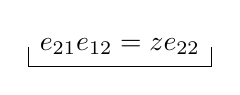
\begin{tikzpicture}
\node (product) [inner sep=4pt] {\(e_{21}e_{12}=ze_{22}\)};
\draw (product.west)--(product.south west)--(product.south east)--(product.east);
\end{tikzpicture}}\endgroup
\end{center}

We want to find finite-dimensional modules for which mult. by \(z\) is a nilpot. operator.
\[
\underline{e_{ii}^{2}=e_{ii}}.
\]
\[
L_i=\{m:\ e_{ii}m=m\}.
\]
\[
M=L_1\oplus L_2\oplus L_3
\]

\SourceFigure{GELFAND-P000723}{diagram-right-directions}{%
\par\begingroup\color{black}\GelfandFitDiagram{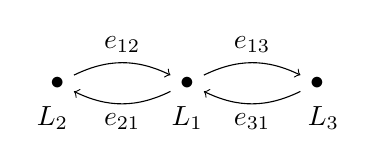
\begin{tikzpicture}[baseline,x=1cm,y=.92cm]
\node (l2) at (0,0) {\(\bullet\)};
\node (l1) at (1.65,0) {\(\bullet\)};
\node (l3) at (3.30,0) {\(\bullet\)};
\node at (-.06,-.48) {\(L_2\)};
\node at (1.65,-.48) {\(L_1\)};
\node at (3.38,-.48) {\(L_3\)};
\draw[->] (l2) to[bend left=26] node[above] {\(e_{12}\)} (l1);
\draw[->] (l1) to[bend left=26] node[below] {\(e_{21}\)} (l2);
\draw[->] (l1) to[bend left=26] node[above] {\(e_{13}\)} (l3);
\draw[->] (l3) to[bend left=26] node[below] {\(e_{31}\)} (l1);
\end{tikzpicture}}\endgroup\par\smallskip
In the manuscript, \(e_{13}\) points from \(L_1\) to \(L_3\), and \(e_{31}\) from \(L_3\) to \(L_1\).}
\end{GelfandAdjacentEvidence}


\[
e_{21}e_{12}=ze_{22}\qquad\text{is nilpotent}
\]
\[
e_{12}e_{21}=ze_{11}=e_{13}e_{31}
\]
hence the categ. of modules over this ring \(\cong\ldots\)

\underline{\uwave{For \(SL(3,\mathbb R)\)}}\qquad
\uwave{the answer is as follows:}
\[
E=\{z_1,z_2\}\qquad\text{in a nbhd. of zero:}
\]
\[
B=\underset{a_{ij}}{M_4}\oplus
\underset{b_{ij}}{M_3}\oplus
\underset{c_{ij}}{M_3}\oplus
\underset{d}{M_1}
\]
\underline{Conditions.}
\[
1)\ \text{At }z_1=0\qquad\left\Vert\quad
\begin{aligned}
a_{13}=a_{14}=a_{23}=a_{24}=b_{12}=b_{13}=0\\
a_{33}=b_{22},\quad a_{34}=b_{23},\quad
a_{43}=b_{32},\quad a_{44}=b_{33}
\end{aligned}\right.
\]


\Needspace{7\baselineskip}
\begin{GelfandAdjacentEvidence}{GELFAND-P000724}{1}
\SourcePage{GELFAND-P000724}{62}
\SourceFigure{GELFAND-P000724}{top-matrix-consistency}{%
\begingroup\color{black}\GelfandFitDiagram{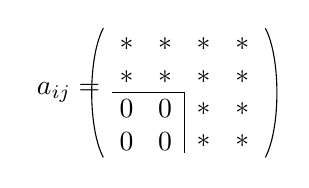
\begin{tikzpicture}[baseline=(current bounding box.center),x=.49cm,y=.41cm]
\node at (-1.5,-1.5) {\(a_{ij}=\)};
\foreach \row in {0,1} {
  \foreach \col in {0,1,2,3} {\node at (\col,-\row) {\(\ast\)};}
}
\foreach \row in {2,3} {
  \foreach \col in {0,1} {\node at (\col,-\row) {\(0\)};}
  \foreach \col in {2,3} {\node at (\col,-\row) {\(\ast\)};}
}
\draw (-.6,.5) .. controls (-1,-.4) and (-1,-2.6) .. (-.6,-3.5);
\draw (3.6,.5) .. controls (4,-.4) and (4,-2.6) .. (3.6,-3.5);
\draw (-.38,-1.5)--(1.5,-1.5)--(1.5,-3.35);
\end{tikzpicture}}\endgroup}
\end{GelfandAdjacentEvidence}
\begin{GelfandAdjacentEvidence}{GELFAND-P000724}{2}

\SourceFigure{GELFAND-P000724}{top-matrix-consistency-right}{%
\begingroup\color{black}\GelfandFitDiagram{\begin{tikzpicture}\node[inner sep=0pt] {\(\begin{pmatrix}\ast&\ast&\ast\\0&\ast&\ast\\0&\ast&\ast\end{pmatrix}\)};\end{tikzpicture}}\endgroup}
\end{GelfandAdjacentEvidence}
\begin{GelfandAdjacentEvidence}{GELFAND-P000724}{3}


\[
2)\ \text{When }z_2=0\qquad\left\Vert\quad
\begin{aligned}
a_{12}=a_{14}=a_{34}=c_{12}=c_{13}=a_{32}=0\\
a_{22}=c_{22},\quad a_{24}=c_{23},\quad
a_{42}=c_{32},\quad a_{44}=c_{33}
\end{aligned}\right.
\]

\[
3)\ \text{When }z_1+z_2=0.\qquad\left\Vert\quad
\begin{aligned}
b_{13}=b_{23}=c_{13}=c_{23}=0;\\
b_{33}=c_{33}.
\end{aligned}\right.
\]
\Unclear{GELFAND-P000724}{condition-three-sign}{The overwritten sign between \(z_1\) and \(z_2\) is tentatively read as \(+\).}
\end{GelfandAdjacentEvidence}



\Needspace{7\baselineskip}
\begin{GelfandAdjacentEvidence}{GELFAND-P000725}{1}
\SourcePage{GELFAND-P000725}{unlabelled}
\underline{24/X--77}

\underline{S. I. Gelfand.}\qquad\underline{Harish-Chandra Modules}

HC modules for
\[
\begin{aligned}
G&=SL(2,\mathbb R)/(\pm1)\\
K&=SO_2/(\pm1)\\[-.25ex]
 &\quad\text{(max. comp. subgroup)}
\end{aligned}
\]

\(\mathfrak g\) --- Lie algebra
\[
\begin{array}{ccc}
E_+,&E_-,&H\\[.4ex]
\begin{pmatrix}0&1\\0&0\end{pmatrix},&
\begin{pmatrix}0&0\\1&0\end{pmatrix},&
\begin{pmatrix}1&0\\0&-1\end{pmatrix}
\end{array}
\qquad\text{--- generators of }\mathfrak g
\]
\[
\begin{array}{cl}
\mathfrak k&\subset\mathfrak g.\\[-.5ex]
\Vert&\\
\multicolumn{2}{l}{\left\{\begin{pmatrix}0&1\\-1&0\end{pmatrix}=X_c\right\}}
\end{array}
\]
\Unclear{GELFAND-P000725}{bottom-generator}{The subscript on \(X\) reads as an open \(c\).}
\end{GelfandAdjacentEvidence}



\Needspace{7\baselineskip}
\begin{GelfandAdjacentEvidence}{GELFAND-P000726}{1}
\SourcePage{GELFAND-P000726}{67}
\uwave{A module} H.--C. --- is a (infinite-dimensional) repr. in [crossed out] \(V\), such that
\Unclear{GELFAND-P000726}{top-cancellation}{The crossed-out fragment before \(V\) is illegible.}
\end{GelfandAdjacentEvidence}
\begin{GelfandAdjacentEvidence}{GELFAND-P000726}{2}


1) \(X_0\) has only integer eigenvalues, and even ones at that

2) [crossed out] each eigenvalue [inserted above: of the operator \(X_0\)] has finite multiplicity
\Unclear{GELFAND-P000726}{item-two-cancellation}{The heavily crossed-out mark after 2) is illegible.}
\end{GelfandAdjacentEvidence}
\begin{GelfandAdjacentEvidence}{GELFAND-P000726}{3}


3) \(V\) is finitely generated (over the envelop. algebra)

(\(\Leftrightarrow\) the eigenvalue multiplicities are bounded).

\(v_1,\ldots,v_n\) --- generators

\begin{quote}
\small \textit{[In the right margin beyond the double line]} 1) --- so that one can integrate to a group repr. (\(e^{inx}\) etc.)
\end{quote}

\uwave{Definition.}\quad \(Z(\mathfrak g)\) --- the centre of the envelop. algebra \(U(\mathfrak g)\)

(gen. by the element \(z=4E_-E_+-H^2+2H\))
\Unclear{GELFAND-P000726}{casimir-sign}{The manuscript has a minus before \(H^2\) and a plus before \(2H\).}
\end{GelfandAdjacentEvidence}
\begin{GelfandAdjacentEvidence}{GELFAND-P000726}{4}


\(\operatorname{supp} V={}\) the set of eigenvalues of the operator \(z\) in \(V\)

\underline{Theorem:} this is a finite set for any \(V\).

\uwave{Definition.} Let \(D\) --- a domain in \(\mathbb C\).
\[
C_D=\{V,\ \operatorname{supp}V\subset D\}
\]
Let \(D\) --- a small neighbourhood of zero (disc of radius \(<1/2\)).
\[
R=\left\{\begin{pmatrix}
a_{11}(\lambda)&a_{12}(\lambda)&a_{13}(\lambda)\\
a_{21}(\lambda)&a_{22}(\lambda)&a_{23}(\lambda)\\
a_{31}(\lambda)&a_{32}(\lambda)&a_{33}(\lambda)
\end{pmatrix}\right.,\quad a_{ij}(\lambda)\text{ --- analytic fns. in }D
\]
\Unclear{GELFAND-P000726}{matrix-index-overwrite}{The first subscript on \(a_{12}(\lambda)\) is overwritten and reads as \(1\).}
\end{GelfandAdjacentEvidence}
\begin{GelfandAdjacentEvidence}{GELFAND-P000726}{5}


\[
a_{ij}(0)=\begin{pmatrix}\ast&0&0\\\ast&\ast&0\\\ast&0&\ast\end{pmatrix}
\]
\Unclear{GELFAND-P000726}{matrix-value-notation}{The left-hand side is written \(a_{ij}(0)\).}
\end{GelfandAdjacentEvidence}
\begin{GelfandAdjacentEvidence}{GELFAND-P000726}{6}


\[
\operatorname{Mod} R=
\left\{\underset{\substack{|\\R\text{-module}}}{M}:\ \dim_{\mathbb C}M<\infty\right\}
\]
\underline{Theorem.} The category \(C_D\) is equivalent to the category \(\operatorname{Mod} R\).

\underline{Example.}

\uwave{The category of modules over the matrix ring is equivalent to the category of} [crossed out: linear\ldots?] \uwave{finite-dimensional linear spaces}
\Unclear{GELFAND-P000726}{cancelled-category}{The crossed-out word tentatively begins “linear”; the ending is uncertain.}
\end{GelfandAdjacentEvidence}
\begin{GelfandAdjacentEvidence}{GELFAND-P000726}{7}


(\(\sim\) a repr. of the matrix alg. is a direct sum)

\(V\) --- the stand. repr. of the alg. \(M_\ell\)
\Unclear{GELFAND-P000726}{matrix-subscript}{The subscript on \(M\) is tentatively read as \(\ell\); the mark also resembles \(e\).}
\end{GelfandAdjacentEvidence}

\[
E\longmapsto V\underset{\mathbb C}{\otimes}E,\qquad
M_\ell\text{ acts on the first variable}
\]
\[
W\text{ --- }M_\ell\text{-module}\quad\longmapsto\quad
E=\operatorname{Hom}_{M_\ell}(V,W).
\]
(the 2 functors giving the equivalence are written out)

Old formulation: \(\forall\, M_\ell\) module decomposes as a direct sum.


\Needspace{7\baselineskip}
\begin{GelfandAdjacentEvidence}{GELFAND-P000727}{1}
\SourcePage{GELFAND-P000727}{unlabelled}
\underline{Proof of the theorem.}

I. Let a list of numbers be given \(n_1,\ldots,n_k\). Construct from it the ring \(Q_{n_1,\ldots,n_k}\)

a) \(J_{n_1\ldots n_k}\) --- the left ideal in \(U(\mathfrak g)\), generated by the element
\[
(X_0-2in_1)(X_0-2in_2)\cdots(X_0-2in_k)
\]

\[
\text{b)}\quad
N_{n_1,\ldots,n_k}=
\{u\in U(\mathfrak g)\mid
J_{n_1,\ldots,n_k}u\subset J_{n_1,\ldots,n_k}\}
\]
(the smallest subalg., in which \(J\) --- a 2-sided ideal
\Unclear{GELFAND-P000727}{normalizer-word}{The manuscript reads “smallest”.}
\end{GelfandAdjacentEvidence}
\begin{GelfandAdjacentEvidence}{GELFAND-P000727}{2}


\[
Q_{n_1\ldots n_k}=N_{n_1,\ldots,n_k}/J_{n_1,\ldots,n_k}
\]

\uuline{Def.}\quad \(V\) --- an H.--C. module
\[
\tau_{n_1,\ldots,n_k}(V)\underset{\mathrm{def}}{=}
\{v:\ (X_0-2in_1)\cdots(X_0-2in_k)v=0\}
\]

This is a finite-dimensional subspace

Dimension \(={}\) sum of the multiplicities

\(N\) maps it into itself

\(J\)\quad --- '' --- \quad to zero
\[
\Rightarrow\quad Q_{n_1,\ldots,n_k}\text{ acts in }\tau_{n_1,\ldots,n_k}(V)
\]

This is [crossed out: construction?], a functor
\Unclear{GELFAND-P000727}{functor-cancellation}{The crossed-out word is tentatively read as “construction”.}
\end{GelfandAdjacentEvidence}
\begin{GelfandAdjacentEvidence}{GELFAND-P000727}{3}

\[
\text{H.--C. modules}\longrightarrow
\text{finite-dimensional modules over }Q_{n_1,\ldots,n_k}
\]
\Unclear{GELFAND-P000727}{overwritten-functor-subscript}{The first mark in the last subscript of \(Q\) is retraced. It reads \(n_k\).}
\end{GelfandAdjacentEvidence}
\begin{GelfandAdjacentEvidence}{GELFAND-P000727}{4}


It is clear that
\[
z\in N_{n_1,\ldots,n_k}
\]
\[
\operatorname{supp} M=\{\text{eigenvalues of }z\}
\]
\[
(\operatorname{Mod} Q_{n_1,\ldots,n_k})_D
\]
(finite-dimensional modules with support in \(D\)).

\SourceFigure{GELFAND-P000727}{bottom-arrow}{%
\par\begingroup\color{black}\GelfandFitDiagram{\begin{tikzpicture}[baseline=(current bounding box.center)]
\draw[<-] (0,0)--(.8,0);
\draw (.8,-.15)--(.8,.15);
\end{tikzpicture}}\endgroup\par\smallskip
The short arrow points left and has a crossbar at the right. Its connection to the adjacent line is uncertain.}
\end{GelfandAdjacentEvidence}


\uwave{Theorem} 1. Let \(D\) --- be any bounded domain in \(\mathbb C^1\).
Then there exist \(n_1,\ldots,n_k\), such that \(C_D\) and
\((\operatorname{Mod} Q_{n_1,\ldots,n_k})_D\) are equiv.


\Needspace{7\baselineskip}
\begin{GelfandAdjacentEvidence}{GELFAND-P000728}{1}
\SourcePage{GELFAND-P000728}{68}
\underline{II.}\quad \underline{Definition of the reprs. of the principal series.}

from \(s\) construct the module \(T^{(s)}=V\)
\[
V=\{\underset{\substack{\text{functions}\\\text{on the plane}}}{f(x,y)}\}
\]
1) \(f(tx,ty)=|t|^sf(x,y)\)

2) \(f(+\sin\varphi,\cos\varphi)=P(\sin\varphi,\cos\varphi)\)
\Unclear{GELFAND-P000728}{plus-sine}{The first argument has a \(+\) before \(\sin\varphi\).}
\end{GelfandAdjacentEvidence}
\begin{GelfandAdjacentEvidence}{GELFAND-P000728}{2}


\(\underline{P}\) --- a polynomial.

The Lie algebra acts in the natural way (diff. operators)

(the group acts on the argument)
\[
E_+\sim x\frac{\partial}{\partial y};\quad
E_-\sim y\frac{\partial}{\partial x};\quad
H\sim x\frac{\partial}{\partial x}-y\frac{\partial}{\partial y}.
\]
Restr. to \(S^1\cong{}\) the space of polynomials (even on the circle)
\[
L_0\simeq T^{(s)}\qquad\text{(for any }s\text{).}
\]
\Unclear{GELFAND-P000728}{l0-degree}{The opening parenthesis in the superscript \((s)\) is heavily retraced.}
\end{GelfandAdjacentEvidence}
\begin{GelfandAdjacentEvidence}{GELFAND-P000728}{3}


\underline{Lemma 1.} Let \(X\in U(\mathfrak g)\). The action of \(X\) depends polynomially on \(s\).

(Matrix entries in the monomial basis are polynomials in \(s\))
\[
\tau_{n_1,\ldots,n_k}(T^{(s)})=L_{n_1,\ldots,n_k}
\]
\underline{Lemma 2.} Let \(q\in Q_{n_1,\ldots,n_k}\). The action of \(q\) depends polynomially on \(s\).

\uwave{Theorem 2.}\quad \uwave{Set}
\[
B_{n_1,\ldots,n_k}=\operatorname{End}(L_{n_1,\ldots,n_k})
\]
Then there exists a map
\[
\psi_{n_1,\ldots,n_k}:
Q_{n_1,\ldots,n_k}\longrightarrow B_{n_1,\ldots,n_k}[s],
\]
\Unclear{GELFAND-P000728}{embedding-symbol}{The symbol for the map is tentatively read as \(\psi\).}
\end{GelfandAdjacentEvidence}
\begin{GelfandAdjacentEvidence}{GELFAND-P000728}{4}


[crossed out: Thm.?] [inserted above: such that] \(\psi\) --- \uwave{an embedding}
\Unclear{GELFAND-P000728}{embedding-cancellation}{The crossed-out heading tentatively reads “Теор.” (Thm.).}
\end{GelfandAdjacentEvidence}
\begin{GelfandAdjacentEvidence}{GELFAND-P000728}{5}


(i.e. the principal series contains as sub- and quotient reprs. \(\forall\) HC modules)

\underline{III.}\quad \uwave{Combining stages I and II.}

\(D\) --- a small nbhd. of zero

\underline{Lemma 0.}

On \(T^{(s)}\) the operator \(z\) is \((-s^2+2s)\operatorname{Id}\)
\Unclear{GELFAND-P000728}{scalar-casimir}{The manuscript gives \((-s^2+2s)\operatorname{Id}\).}
\end{GelfandAdjacentEvidence}
\begin{GelfandAdjacentEvidence}{GELFAND-P000728}{6}


\(z=0\) for \(s=0\) and \(s=2\).

\underline{Lemma 1.} Let \(s\) be near the point 0.

1) Then \(T^s\), \(s\ne 0\) is irreducible
\[
0\longrightarrow\operatorname{Id}\longrightarrow T^{(0)}
\longrightarrow T_+\oplus T_-\longrightarrow 0
\]
\Unclear{GELFAND-P000728}{identity-overtrace}{The second letter of \(\operatorname{Id}\) is heavily retraced.}
\end{GelfandAdjacentEvidence}

and the exact seq. does not split


\Needspace{7\baselineskip}
\begin{GelfandAdjacentEvidence}{GELFAND-P000729}{1}
\SourcePage{GELFAND-P000729}{unlabelled}
\[
2)\quad T^{(s)}\big|_K=\bigoplus_{j=-\infty}^{\infty}\delta_j.
\]
\(\delta_k={}\) eigensp. of \(X_0\) with eigenval. \(2ik\).

(1-dimensional repr.)
\[
I\big|_K=\delta_0,\qquad
T_+\big|_K=\bigoplus_{j>0}\delta_j,\qquad
T_-\big|_K=\bigoplus_{j<0}\delta_j.
\]
\Unclear{GELFAND-P000729}{right-edge-mark}{A narrow mark resembling \(I\) is visible beyond the right border. Its connection to the text is uncertain.}
\end{GelfandAdjacentEvidence}
\begin{GelfandAdjacentEvidence}{GELFAND-P000729}{2}


[In the left margin: В?] \underline{Lemma 2.} Near \(s=2\)
\Unclear{GELFAND-P000729}{lemma-margin-letter}{The heavily retraced mark in the margin tentatively reads “В”.}
\end{GelfandAdjacentEvidence}
\begin{GelfandAdjacentEvidence}{GELFAND-P000729}{3}

\[
0\longrightarrow T_+\oplus T_-\longrightarrow T^{(2)}\longrightarrow I\longrightarrow0
\]
\(T^{(s)}\), \(s\ne2\) is irreducible

\underline{Lemma 3.}\quad \(s\ne0\qquad T^{(s)}\simeq T^{(2-s)}\)

\(s\) near zero
\Unclear{GELFAND-P000729}{lemma-three-superscript}{The opening parenthesis in the superscript of \(T^{(s)}\) is retraced.}
\end{GelfandAdjacentEvidence}
\begin{GelfandAdjacentEvidence}{GELFAND-P000729}{4}


Consider the numbers \((n_1,n_2,n_3)=(-1,0,1)\) and the ring
\[
Q_{(-1,0,1)}
\]
\(D\) --- a suff. small nbhd. of zero \(\qquad\Rightarrow\quad C_D\sim Q_{(-1,0,1)}\)

(\underline{explanation:} in \(T_+\) there is a repr. with \(+1\), in \(T_-\) --- '' --- with \(-1\) etc.)
\[
\tau_{-1,0,1}(T^{(s)})=\{e_{-1},e_0,e_1\}
\]
\(q\in Q_{-1,0,1}\)

\par\smallskip\noindent\dotfill\par\smallskip

\underline{Done}:\quad \(SL(2,\mathbb R)/(\pm1)\), \(SL(2,\mathbb R)\), \(PGL(2,\mathbb R)\),

\(SL(2,\mathbb C)\), \(SL(3,\mathbb R)\)

Probably possible \(SL(3,\mathbb C)\) and \(SU(2,1)\)

Recommended, calc. \(SO(4,1)\) (easy), \(Sp(4,\mathbb C)\) (easy)

Difficult: \(SL(4,\mathbb R)/(\pm1)\), \(SL(4,\mathbb C)\).

Read the works of Hirai, Zhelobenko

Gelfand, Graev

\underline{Krichever}

\uwave{2 minutes for a sensational announcement.}

[In the left margin: \uwave{On eqns.?}]
\[
[L_1,L_2]=0
\]
\Unclear{GELFAND-P000729}{margin-abbreviation}{The Russian abbreviation tentatively reads “Об ур-и”, possibly “Об ур-й”.}
\end{GelfandAdjacentEvidence}
\begin{GelfandAdjacentEvidence}{GELFAND-P000729}{5}


Coddington pointed to the works of

\uwave{Burchnal}, \uwave{Chaundy}\quad
\href{https://doi.org/10.1112/plms/s2-21.1.420}{1922},
\href{https://doi.org/10.1098/rspa.1928.0069}{1928},
\href{https://doi.org/10.1098/rspa.1931.0208}{1931}

and \uwave{Baker} [crossed out] \href{https://doi.org/10.1098/rspa.1928.0070}{1928}
\Unclear{GELFAND-P000729}{baker-cancellation}{The writing between “Baker” and “1928” is heavily crossed out.}
\end{GelfandAdjacentEvidence}


[To the right of the list of works:] --- they objected to Baker, who recommended using alg. geom.

The problem of describing commuting ops. with scalar coeffs. of relatively prime ord. was posed and solved.

the answer uses no \(\Theta\)-fns. and is insufficiently effective

the 1st was found via Lamé fns. (as in Akhiezer). they did not see the straight-line behav.


\Needspace{7\baselineskip}
\begin{GelfandAdjacentEvidence}{GELFAND-P000730}{1}
\SourcePage{GELFAND-P000730}{69}
path on the Jacobian (and even conditional periodicity).

Forgotten --- in the 1939 paper there are no longer any references.

\SourceFigure{GELFAND-P000730}{proceedings-brackets}{%
\par\begingroup\color{black}\GelfandFitDiagram{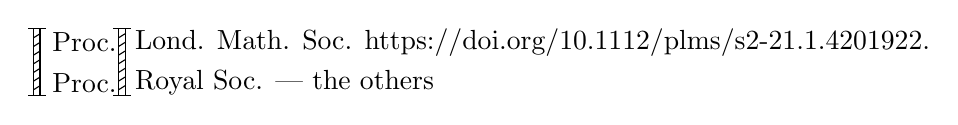
\begin{tikzpicture}[x=1cm,y=1cm]
\foreach \x in {0,1.08} {
 \draw (\x,-.43) rectangle ++(.08,.86);
 \draw (\x-.07,.43)--++(.23,0) (\x-.07,-.43)--++(.23,0);
 \foreach \y in {-.35,-.24,-.13,-.02,.09,.20,.31}
  {\draw (\x,\y)--++(.08,.05);}
}
\node[anchor=west,inner sep=0pt] at (.23,.25) {Proc.};
\node[anchor=west,inner sep=0pt] at (.23,-.26) {Proc.};
\node[anchor=west,inner sep=0pt,text=black] at (1.28,.25)
  {Lond. Math. Soc. \href{https://doi.org/10.1112/plms/s2-21.1.420}{1922}.};
\node[anchor=west,inner sep=0pt,text=black] at (1.28,-.26)
  {Royal Soc. --- the others};
\end{tikzpicture}}\endgroup\par}
\end{GelfandAdjacentEvidence}
\begin{GelfandAdjacentEvidence}{GELFAND-P000730}{2}


almost commuting [crossed out] and Lax pairs \uuline{exist}.
\Unclear{GELFAND-P000730}{lax-cancellation}{A small mark after “almost commuting” is crossed out.}
\end{GelfandAdjacentEvidence}
\begin{GelfandAdjacentEvidence}{GELFAND-P000730}{3}


[crossed out] \underline{31/X--77}\quad \underline{Gelfand Sem.}\quad
\uuline{S. P. Novikov.}\quad \uuline{Instantons.}
\Unclear{GELFAND-P000730}{date-cancellation}{The heavily crossed-out mark before the date is illegible.}
\end{GelfandAdjacentEvidence}
\begin{GelfandAdjacentEvidence}{GELFAND-P000730}{4}


\[
\mathbb R^4\subset S^4\qquad(|x|\to\infty)
\]
\[
A=\text{[crossed out]}\ A_\mu\,dx^\mu
\qquad\text{connection form}
\]
\Unclear{GELFAND-P000730}{connection-cancellation}{The crossed-out expression after \(A=\) appears to contain \(A\) and \(d\). The indices are illegible.}
\end{GelfandAdjacentEvidence}
\begin{GelfandAdjacentEvidence}{GELFAND-P000730}{5}


If the curvature is 0, then
\[
(1)\qquad A_\mu\longrightarrow\frac{\partial g}{\partial x^\mu}\,g^{-1}(x),
\qquad g(x)\in G
\]
\[
A_\mu(x)\in L_G\qquad\text{(Lie algebra)}
\]
Curvature form:
\[
(2)\qquad F_{\nu\mu}=dA+[A,A]=\mathcal D A
\]
(covariant derivative)

Most often \(G=SU_2\) (Yang--Mills).

\([A,A]\) --- exterior prod., but mult. of coeffs. is in the Lie alg..

Other notation: \(A\wedge A=[A,A]\), \(\mathcal D A=\nabla_A A\)

The requirement that everything be on \(S^4\) --- is slightly stronger than finite energy.

(\underline{Rem.} Nonlinear (chiral) fields \(\leftrightarrow\) connection with zero curvature;
given by fns. with values in the group.)

Set
\[
(3)\qquad n=P(A)=\frac12\int\varepsilon_{abcd}F^{ab}F^{cd}\,d^4x
\]
\Unclear{GELFAND-P000730}{topological-integral}{Equation (3) has no written trace symbol before the product \(F^{ab}F^{cd}\).}
\end{GelfandAdjacentEvidence}
\begin{GelfandAdjacentEvidence}{GELFAND-P000730}{6}

(char. Chern class --- top. invariant --- an integer up to a factor \(\frac{\pi^2}{16}\)).
\Unclear{GELFAND-P000730}{chern-factor}{The denominator of the fraction is tentatively read as \(16\).}
\end{GelfandAdjacentEvidence}
\begin{GelfandAdjacentEvidence}{GELFAND-P000730}{7}


\[
(4)\qquad S(A)=\frac1{g_c}\int_{\mathbb R^4}
       \operatorname{Sp}(F_{\mu\nu}F^{\mu\nu})\,d^4x
\]
\Unclear{GELFAND-P000730}{coupling-subscript}{The open subscript on \(g\) tentatively reads \(c\), possibly \(0\).}
\end{GelfandAdjacentEvidence}
\begin{GelfandAdjacentEvidence}{GELFAND-P000730}{8}

(Yang--Mills functional)

\uwave{Class. electrodynamics} --- \(G=SU(1)\) or \(\mathbb R\)
\Unclear{GELFAND-P000730}{electrodynamics-group}{The manuscript reads \(SU(1)\).}
\end{GelfandAdjacentEvidence}
\begin{GelfandAdjacentEvidence}{GELFAND-P000730}{9}


depending on whether there are real charges or not.
\Unclear{GELFAND-P000730}{charges-adjective}{The faint abbreviation before “charges” tentatively reads “реал.” (real).}
\end{GelfandAdjacentEvidence}


Yang--Mills eqns.:
\[
(5)\qquad \delta S=0.
\]
Class. problem: find all such \(A\), that \(S(A)<+\infty\).

\underline{Rem.} The metric of \(S^4\) is conformally equiv. to the metric of \(\mathbb R^4\),
\[
g_{\mu\nu}(y)=g(y)\delta_{\mu\nu}
\]
The Maxwell and Yang--Mills eqns. are \uwave{conformally invariant}.

Grp. of conformal transfs. of Euclidean sp. and the sphere \(\qquad\Vert\qquad O(5,1)=K_4\)


\Needspace{7\baselineskip}
\begin{GelfandAdjacentEvidence}{GELFAND-P000731}{1}
\SourcePage{GELFAND-P000731}{unlabelled}
Solutions are mult. by a scalar under the action of the conformal group:
\[
f:X\longrightarrow X,\qquad f^*(g_{ij})=g(x)g_{ij}.
\]
(continuous conf. transfs.)
\Unclear{GELFAND-P000731}{parenthesis-word}{The first word in parentheses tentatively reads “continuous”.}
\end{GelfandAdjacentEvidence}
\begin{GelfandAdjacentEvidence}{GELFAND-P000731}{2}


[crossed out: Cont. bund. into?]
\Unclear{GELFAND-P000731}{top-cancellation}{The crossed-out line tentatively reads “Непр. рассл. в” (Cont. bund. into).}
\end{GelfandAdjacentEvidence}
\begin{GelfandAdjacentEvidence}{GELFAND-P000731}{3}


A cont. map of bases takes a bundle to a bundle and a connection to a connection.
Then the new connection again satisfies the Yang--Mills eqn..

\(\underline{\underline{O(5,1)}}\)

On the sphere \(S^4\) there is \(O(5)\)

Stereogr. transf. \(S^4\) onto \(\mathbb R^4\) and in \(\mathbb R^4\) take similarity transfs..

Where does \(O(5,1)\)?

We must consider the cone
\[
\underline{x_1^2+x_2^2+\cdots+x_5^2-x_6^2=0.}
\]
\SourceFigure{GELFAND-P000731}{null-cone-diagram}{%
\par\begingroup\color{black}\GelfandFitDiagram{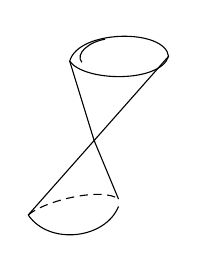
\begin{tikzpicture}[x=1.55cm,y=1.55cm]
\draw (-.20,.65) .. controls (-.13,.91) and (.58,.92) .. (.61,.69)
 .. controls (.54,.47) and (-.08,.48) .. (-.20,.65);
\draw (-.10,.64) .. controls (-.16,.71) and (-.04,.81) .. (.09,.83);
\draw (-.20,.65)--(0,0)--(.20,-.48);
\draw (.61,.69)--(0,0)--(-.54,-.61);
\draw (-.54,-.61) .. controls (-.37,-.86) and (.09,-.81) .. (.20,-.54);
\draw[densely dashed] (-.54,-.61) .. controls (-.40,-.49) and (.07,-.38) .. (.20,-.48);
\end{tikzpicture}}\endgroup\par}
\end{GelfandAdjacentEvidence}
\begin{GelfandAdjacentEvidence}{GELFAND-P000731}{4}

[undeciphered mark] and lin. transfs. preserving the cone.
\Unclear{GELFAND-P000731}{cone-caption-symbol}{The isolated mark before “and” is illegible.}
\end{GelfandAdjacentEvidence}
\begin{GelfandAdjacentEvidence}{GELFAND-P000731}{5}


The rays of the cone --- \(S^4\). The transfs. are conformal on \(S^4\).

The conformal group preserves the functional \(S(A)\)

\uwave{Belavin--Polyakov instantons.}
\[
(6)\qquad \min_{P(A)=n}S(A)=n.\qquad \text{(when }g_c=1\text{)}
\]
\Unclear{GELFAND-P000731}{coupling-condition}{The subscript on \(g\) is tentatively read as \(c\), possibly \(0\).}
\end{GelfandAdjacentEvidence}
\begin{GelfandAdjacentEvidence}{GELFAND-P000731}{6}


and in fact the minima satisfy the eqn. [crossed out]
\Unclear{GELFAND-P000731}{equation-cancellation}{The crossed-out expression resembles \(F={*}F\); the middle signs are uncertain.}
\end{GelfandAdjacentEvidence}
\begin{GelfandAdjacentEvidence}{GELFAND-P000731}{7}

\[
(7)\qquad \underline{F={*}F}
\]
(duality eqns.)

(\href{https://doi.org/10.1016/0370-2693(75)90163-X}{Belavin and Polyakov})

And conversely, solns. of these eqns. with given \(n\) --- realize a strict minimum in the given class.

A number of authors gave explicit solns. (for \(\forall\,n\) at least one solution exists).

[crossed out: Ger?] \underline{t' Hooft} found explicit fmlas. for \(\underline{n=2}\). (all solutions!)
\Unclear{GELFAND-P000731}{hooft-cancellation}{The crossed-out fragment before the surname tentatively reads “Гер” (Ger).}
\end{GelfandAdjacentEvidence}
\begin{GelfandAdjacentEvidence}{GELFAND-P000731}{8}


by means of an elem. substitution.

The solutions form an \((8n-3)\)-dimensional manifold
(Schwarz, from the Atiyah--Singer thm.). This is \(M^{8n-3}\).

Atiyah--Singer 3 months later.

t' Hooft found [crossed out] a manifold of dimension \(\underline{\underline{5n+4}}\). (\(n\geq3\))
\Unclear{GELFAND-P000731}{family-cancellation}{The short crossed-out entry after “found” is illegible.}
\end{GelfandAdjacentEvidence}
\begin{GelfandAdjacentEvidence}{GELFAND-P000731}{9}


For \(n=2\) they coincide. It is unclear whether there is another connected component.

\underline{Proof of Schwarz’s thm.}

Linearize eqns. (7):
\[
(A_\mu)\longrightarrow A_\mu+a_\mu=A+\delta A
\]
linearized operator\quad \(a_\mu\longrightarrow Ta_\mu\)
\Unclear{GELFAND-P000731}{final-speck}{An isolated, undeciphered trace is visible to the right of \(Ta_\mu\).}
\end{GelfandAdjacentEvidence}



\Needspace{7\baselineskip}
\begin{GelfandAdjacentEvidence}{GELFAND-P000732}{1}
\SourcePage{GELFAND-P000732}{70}
\[
\begin{aligned}
B(A)&=F-{*}F=0,\\
B(A+\delta A)&=T(\delta A)+O((\delta A)^2)
\end{aligned}
\]
\uwave{Counting the index}: \(cn\) --- a linear fn. of \(n\); compute the vals. at \(0\) and \(1\).

\uuline{Cokernel \(=0\)}\quad [crossed out]\quad \(\Leftarrow\) Hopf considerations.
\Unclear{GELFAND-P000732}{index-cancellation}{A passage after “Cokernel = 0” is heavily crossed out. A left-pointing arrow is visible at right.}
\end{GelfandAdjacentEvidence}
\begin{GelfandAdjacentEvidence}{GELFAND-P000732}{2}


Obtain \(\underline{\underline{8n}}\): 3 parameters redundant due to gauge \underline{invariance}.

Use of the conf. group \(\Rightarrow\) For \(n=1\) all solns. are spher. symmetric.

\(O(5,1)\) acts on the set of solns.

\uwave{For \(n=1\) the set of solns. is 5-dim.}\qquad [At right:] \(\dim O(5,1)=15\).

on \(\forall\) conn. comp. acts \(O(5,1)\).

Hence the stab. subgroup has dim. \(\geq10\). But \(>10\) is impossible, since the stab. subgroup is compact (there is a metric)

\(\Rightarrow\) they are homog. spaces for \(SO(5)\), i.e. spher. symmetric.

(spher. symm. up to gauge invariance).

2-instant. --- still incomplete.

Method of \uwave{Atiyah} and \uwave{Zakharov--Belavin}

Cond. \(\underline{F={*}F}\).

we want to express it as a cond. of commutativity of diff. operators
\[
\left(\text{e.g., }\left[L-\frac{\partial}{\partial t},\
 A-\frac{\partial}{\partial y}\right]=0\right)
\]
\underline{Theorem}
\[
(8)\quad [\widehat B_1(\lambda),\widehat B_2(\lambda)]=0,\ \forall\lambda
\quad\Longleftrightarrow\quad\text{duality eqns. (7)}.
\]
(1st order in \(\lambda\)).

[At right, \(\Vert\)] (Zakharov, Belavin, Yang).

Single out solns. by assuming rationality and nonsingularity.
\Unclear{GELFAND-P000732}{solution-qualifier}{The words after “Single out solns.” tentatively read “гипотезой рац.” (by assuming rationality).}
\end{GelfandAdjacentEvidence}
\begin{GelfandAdjacentEvidence}{GELFAND-P000732}{3}

\SourceFigure{GELFAND-P000732}{complex-coordinate-labels}{%
\par\begingroup\color{black}\GelfandFitDiagram{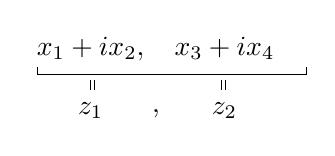
\begin{tikzpicture}[x=1cm,y=1cm]
\node at (.68,.30) {\(x_1+i x_2,\)};
\node at (2.38,.30) {\(x_3+i x_4\)};
\draw (0,.07)--(0,-.03)--(3.42,-.03)--(3.42,.07);
\draw (.68,-.10)--(.68,-.22) (.73,-.10)--(.73,-.22);
\draw (2.34,-.10)--(2.34,-.22) (2.39,-.10)--(2.39,-.22);
\node at (.68,-.48) {\(z_1\)};
\node at (1.51,-.52) {,};
\node at (2.38,-.48) {\(z_2\)};
\end{tikzpicture}}\endgroup\par}
\end{GelfandAdjacentEvidence}
\begin{GelfandAdjacentEvidence}{GELFAND-P000732}{4}


\(B_j(\lambda)\) themselves write as covar. diff. operators.
\[
(9)\quad \widehat B_1(\lambda)=\lambda\nabla_1+\overline{\nabla}_2,\qquad
\widehat B_2(\lambda)=\lambda\nabla_2+\overline{\nabla}_1.
\]
\Unclear{GELFAND-P000732}{lax-sign}{Both operators in (9) have a written \(+\) before the conjugate derivative.}
\end{GelfandAdjacentEvidence}
\begin{GelfandAdjacentEvidence}{GELFAND-P000732}{5}

\[
(10)\quad
\nabla_1=A_1+iA_2+\frac{\partial}{\partial z_1},\qquad
\nabla_2=A_3+iA_4+\frac{\partial}{\partial z_2}.
\]
Connection \(=\{A_1,A_2,A_3,A_4\}\).

The set of complex structures in \(\mathbb R^4\) (linear) is indexed by one complex param. \(\lambda\).
(In fact \(\lambda\) runs through all complex structures).
\Unclear{GELFAND-P000732}{complex-structures}{The parentheses say “all complex structures”. No further restriction is written here.}
\end{GelfandAdjacentEvidence}



\Needspace{7\baselineskip}
\begin{GelfandAdjacentEvidence}{GELFAND-P000733}{1}
\SourcePage{GELFAND-P000733}{unlabelled}
\uwave{Atiyah.}

(approach, did more)
\SourceFigure{GELFAND-P000733}{top-arrow}{%
\par\begingroup\color{black}\GelfandFitDiagram{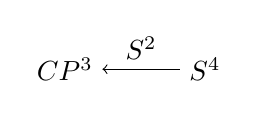
\begin{tikzpicture}[x=1cm,y=1cm]
\node (c) at (0,0) {\(\mathbb C P^3\)};
\node (s) at (1.78,0) {\(S^4\)};
\draw[<-] (c)-- node[above] {\(S^2\)} (s);
\end{tikzpicture}}\endgroup\par
The arrow in the upper line points left.}
\end{GelfandAdjacentEvidence}
\begin{GelfandAdjacentEvidence}{GELFAND-P000733}{2}

(Hopf fibr.)

\SourceFigure{GELFAND-P000733}{hopf-composition}{%
\par\begingroup\color{black}\GelfandFitDiagram{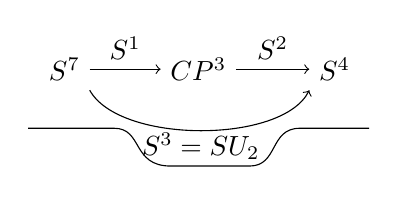
\begin{tikzpicture}[x=1cm,y=1cm]
\node (a) at (0,0) {\(S^7\)};
\node (b) at (1.7,0) {\(\mathbb C P^3\)};
\node (c) at (3.43,0) {\(S^4\)};
\draw[->] (a)--node[above]{\(S^1\)}(b);
\draw[->] (b)--node[above]{\(S^2\)}(c);
\draw[->] (a.south east) .. controls (.7,-.95) and (2.77,-.95) .. (c.south west);
\node at (1.73,-.98) {\(S^3=SU_2\)};
\draw (-.46,-.75)--(.63,-.75) .. controls (1,-.75) and (.85,-1.23) .. (1.35,-1.23)
 --(2.35,-1.23) .. controls (2.72,-1.23) and (2.6,-.75) .. (2.99,-.75)--(3.87,-.75);
\end{tikzpicture}}\endgroup\par}
\end{GelfandAdjacentEvidence}
\begin{GelfandAdjacentEvidence}{GELFAND-P000733}{3}


Important:
\Unclear{GELFAND-P000733}{fibration-heading}{The heading tentatively reads “Важно” (Important).}
\end{GelfandAdjacentEvidence}
\begin{GelfandAdjacentEvidence}{GELFAND-P000733}{4}

\SourceFigure{GELFAND-P000733}{quaternion-fibration}{%
\par\begingroup\color{black}\GelfandFitDiagram{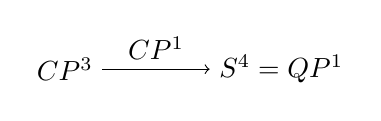
\begin{tikzpicture}[x=1cm,y=1cm]
\node (c) at (0,0) {\(\mathbb C P^3\)};
\node (s) at (2.75,0) {\(S^4=\mathbb Q P^1\)};
\draw[->] (c)--node[above]{\(\mathbb C P^1\)}(s);
\end{tikzpicture}}\endgroup\par}
\end{GelfandAdjacentEvidence}
\begin{GelfandAdjacentEvidence}{GELFAND-P000733}{5}


\(q_1,q_2\) --- quaternions.
\[
q_1=(z_1,z_2),\qquad q_2=(z_3,z_4).
\]
\[
\vec z=e^{i\varphi}\vec z,\qquad
\vec q\to e^{ik}\vec q,\qquad |e^{ik}|=1.
\]
\Unclear{GELFAND-P000733}{complex-action-equality}{There is an equals sign between \(\vec z\) and the exponential.}
\end{GelfandAdjacentEvidence}
\begin{GelfandAdjacentEvidence}{GELFAND-P000733}{6}

\Unclear{GELFAND-P000733}{quaternion-exponent}{After \(i\) in the exponent, the sign is tentatively \(k\). It also resembles \(\kappa\).}
\end{GelfandAdjacentEvidence}
\begin{GelfandAdjacentEvidence}{GELFAND-P000733}{7}


(unit quaternion; they form the grp. \(SU_2\)).
\[
\left(\underset{\text{quatern.}}{\underline{z_1,z_2}}\ \middle|\
\underset{\text{quatern.}}{\underline{z_3,z_4}}\right).
\]
The conn. \(A\) on \(S^4\) we lift to [crossed out: bund.?]
[inserted above in a circle: conn.] [inserted below in a circle: \(\widetilde A\)] on \(\mathbb C P^3\).
\Unclear{GELFAND-P000733}{connection-cancellation}{The crossed-out word is tentatively “рассл.” (bund.). The insertions are circled.}
\end{GelfandAdjacentEvidence}
\begin{GelfandAdjacentEvidence}{GELFAND-P000733}{8}


Connection with grp. \(SU_2\).
\[
SU_2=G
\]
\Unclear{GELFAND-P000733}{group-relation}{The sign before \(G\) tentatively reads \(=\). The lower stroke is heavily retraced.}
\end{GelfandAdjacentEvidence}
\begin{GelfandAdjacentEvidence}{GELFAND-P000733}{9}


The connection gives rise to an almost complex structure.

(the fibres are compl., and in the horiz. sps. it is lifted from the base).

\uwave{Fibre \(\mathbb C^2\).}

Integrability of the almost compl. struct. \(\Longleftrightarrow\) duality eqns..

\(\Longleftrightarrow\) the ops. \(\dfrac{\partial}{\partial z}\) commute.
(repr. as a commuting pair)

\uwave{Recapitulation.}
\SourceFigure{GELFAND-P000733}{repeated-fibration}{%
\par\begingroup\color{black}\GelfandFitDiagram{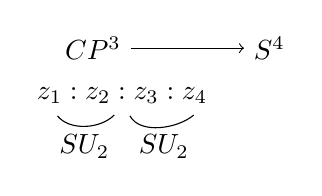
\begin{tikzpicture}[x=1cm,y=1cm]
\node (c) at (.48,0) {\(\mathbb C P^3\)};
\node (s) at (2.72,0) {\(S^4\)};
\draw[->] (c)--(s);
\node at (.85,-.6) {\(z_1:z_2:z_3:z_4\)};
\draw (.03,-.86) .. controls (.18,-1.05) and (.57,-1.03) .. (.75,-.85);
\draw (.95,-.86) .. controls (1.08,-1.10) and (1.56,-1.02) .. (1.76,-.85);
\node at (.37,-1.25) {\(SU_2\)};
\node at (1.38,-1.25) {\(SU_2\)};
\end{tikzpicture}}\endgroup\par}
\end{GelfandAdjacentEvidence}
\begin{GelfandAdjacentEvidence}{GELFAND-P000733}{10}

we act here and there by the same transfs. from \(SU_2\).

[crossed out: \(SU_2\ldots\mathbb C P^3\)?]
\Unclear{GELFAND-P000733}{bottom-cancellation}{The crossed-out expression tentatively contains \(SU_2\) and \(\mathbb C P^3\). The sign between them is uncertain.}
\end{GelfandAdjacentEvidence}


\[
\text{Fibre}=SU_2/(\text{diag. matrices})=\mathbb C P^1.
\]
There is a complex structure in the base and in the fibre.

Suppose on \(M^{2n}\) there is an almost compl. structure

(a way of making \(\forall\) tangent sp. complex)
\[
\begin{gathered}
\partial_1,\ldots,\partial_n\text{ --- a basis of vectors in the tangent sp.}\\
\partial_{n+1},\ldots,\partial_{2n}
\end{gathered}
\]


\Needspace{7\baselineskip}
\begin{GelfandAdjacentEvidence}{GELFAND-P000734}{1}
\SourcePage{GELFAND-P000734}{71}
Let \(\nabla_j=\partial_j+i\partial_{n+j}\)
\[
\frac{\partial}{\partial y_\mu}\equiv i\frac{\partial}{\partial x_\mu}
\]
\Unclear{GELFAND-P000734}{coordinate-relation}{The manuscript uses a three-bar sign \(\equiv\) between the derivatives.}
\end{GelfandAdjacentEvidence}
\begin{GelfandAdjacentEvidence}{GELFAND-P000734}{2}

Req. that they \uwave{commute}.

This is precisely integrability of the almost compl. structure.
\Unclear{GELFAND-P000734}{integrability-overwrite}{The middle letters of the Russian abbreviation “квазикомпл.” (almost complex) are heavily retraced.}
\end{GelfandAdjacentEvidence}



\Needspace{7\baselineskip}
\begin{GelfandAdjacentEvidence}{GELFAND-P000735}{1}
\SourcePage{GELFAND-P000735}{unlabelled}
\noindent\underline{15/XI-77.}\hspace{2em}\underline{Gelfand Sem.}

\underline{B. Sz.-Nagy.}

A number of operator problems reduce to constructing contraction operators on \uwave{Hardy} spaces.
\Unclear{GELFAND-P000735}{opening-first-word}{The faint first word tentatively reads “Ряд” (a number of).}
\end{GelfandAdjacentEvidence}
\begin{GelfandAdjacentEvidence}{GELFAND-P000735}{2}

\Unclear{GELFAND-P000735}{opening-second-word}{The second word tentatively reads “зад.” (problems).}
\end{GelfandAdjacentEvidence}
\begin{GelfandAdjacentEvidence}{GELFAND-P000735}{3}

\Unclear{GELFAND-P000735}{opening-compressed}{The abbreviation following “constructing” tentatively reads “сжат.” (contraction).}
\end{GelfandAdjacentEvidence}
\begin{GelfandAdjacentEvidence}{GELFAND-P000735}{4}


\(H^\infty\) --- bounded analytic functions in the disk.

[Crossed out] \uwave{inner function}
\[
\underset{\mathrm{def}}{=}\quad |u\cdot e^{it}|=1
\]
\hspace*{2em} almost everywhere
\Unclear{GELFAND-P000735}{cancel-before-inner}{The crossed-out signs before “inner function” are illegible.}
\end{GelfandAdjacentEvidence}
\begin{GelfandAdjacentEvidence}{GELFAND-P000735}{5}

\Unclear{GELFAND-P000735}{boundary-product}{The manuscript places a dot between \(u\) and \(e^{it}\).}
\end{GelfandAdjacentEvidence}
\begin{GelfandAdjacentEvidence}{GELFAND-P000735}{6}


\[
\bigwedge_\alpha u_\alpha
\]
--- greatest inner divisor of a family of functions

\Unclear{GELFAND-P000735}{margin-right-curve}{A short curved stroke in the right margin. Its purpose is unclear.}
\end{GelfandAdjacentEvidence}
\begin{GelfandAdjacentEvidence}{GELFAND-P000735}{7}

Blaschke decompos.:
\[
\forall\quad\text{[Crossed out]}\quad u=u_i u_o
\]
\hspace*{2em} (Smirnov thm.)
\Unclear{GELFAND-P000735}{cancel-before-factorization}{The crossed-out signs between \(\forall\) and \(u\) are illegible.}
\end{GelfandAdjacentEvidence}
\begin{GelfandAdjacentEvidence}{GELFAND-P000735}{8}

\Unclear{GELFAND-P000735}{outer-factor-subscript}{The last subscript tentatively reads \(o\).}
\end{GelfandAdjacentEvidence}
\begin{GelfandAdjacentEvidence}{GELFAND-P000735}{9}


\SourceFigure{GELFAND-P000735}{blaschke-diagram}{%
\par\begingroup\color{black}\GelfandFitDiagram{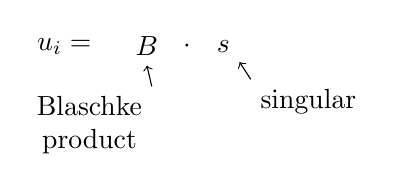
\begin{tikzpicture}[x=1cm,y=1cm]
\node at (0,0) {\(u_i=\)};
\node (b) at (1.05,0) {\(B\)};
\node at (1.56,0) {\(\cdot\)};
\node (s) at (2.02,0) {\(s\)};
\node (bl) at (.32,-1) [align=center] {Blaschke\\product};
\node (sl) at (3.10,-.70) {singular};
\draw[->] (bl.north east) -- (b.south);
\draw[->] (sl.north west) -- (s.south east);
\end{tikzpicture}}\endgroup\par}
\end{GelfandAdjacentEvidence}
\begin{GelfandAdjacentEvidence}{GELFAND-P000735}{10}


of functions with a common zero and by meas. [Crossed out].
\Unclear{GELFAND-P000735}{bottom-abbreviation}{The last Russian abbreviation tentatively reads “мас.”. Its expansion is uncertain.}
\end{GelfandAdjacentEvidence}
\begin{GelfandAdjacentEvidence}{GELFAND-P000735}{11}

\Unclear{GELFAND-P000735}{bottom-cancelled-group}{The crossed-out group at the end of the line is illegible.}
\end{GelfandAdjacentEvidence}



\Needspace{7\baselineskip}
\begin{GelfandAdjacentEvidence}{GELFAND-P000736}{1}
\SourcePage{GELFAND-P000736}{unlabelled}
\SourceFigure{GELFAND-P000736}{singular-measure}{%
\par\begingroup\color{black}\GelfandFitDiagram{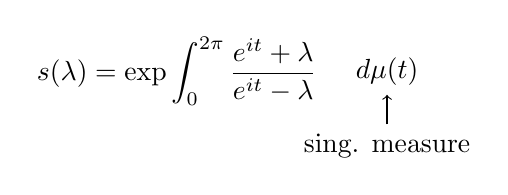
\begin{tikzpicture}[x=1cm,y=1cm]
\node at (0,0) {\(\displaystyle s(\lambda)=\exp\int_0^{2\pi}\frac{e^{it}+\lambda}{e^{it}-\lambda}\)};
\node (measure) at (2.67,0) {\(d\mu(t)\)};
\node (label) at (2.67,-.95) {sing. measure};
\draw[->] (label.north)--(measure.south);
\end{tikzpicture}}\endgroup\par}
\end{GelfandAdjacentEvidence}
\begin{GelfandAdjacentEvidence}{GELFAND-P000736}{2}

\Unclear{GELFAND-P000736}{initial-s-case}{The initial sign tentatively reads \(s\). Its case is uncertain.}
\end{GelfandAdjacentEvidence}
\begin{GelfandAdjacentEvidence}{GELFAND-P000736}{3}


\SourceFigure{GELFAND-P000736}{divisor-labels}{%
\par\begingroup\color{black}\GelfandFitDiagram{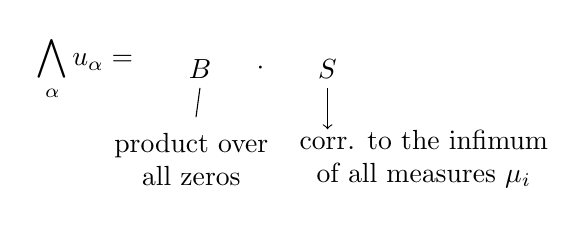
\begin{tikzpicture}[x=1cm,y=1cm]
\node at (0,0) {\(\displaystyle\bigwedge_\alpha u_\alpha=\)};
\node (b) at (1.46,0) {\(B\)};
\node at (2.23,0) {\(\cdot\)};
\node (s) at (3.08,0) {\(S\)};
\node (zeros) at (1.35,-1.15) [align=center] {product over\\all zeros};
\node[anchor=west] (lower) at ([xshift=1.5mm]zeros.east) [align=center] {corr. to the infimum\\of all measures \(\mu_i\)};
\draw (b.south)--++(-.05,-.37);
\draw[->] (s.south)--(3.08,-.77);
\end{tikzpicture}}\endgroup\par}
\end{GelfandAdjacentEvidence}
\begin{GelfandAdjacentEvidence}{GELFAND-P000736}{4}

\Unclear{GELFAND-P000736}{factor-s-case}{The second factor tentatively reads capital \(S\).}
\end{GelfandAdjacentEvidence}
\begin{GelfandAdjacentEvidence}{GELFAND-P000736}{5}


In the Hardy alg. it is false that
\[
u\wedge v=xu+yv.
\]
It is false even that

\SourceFigure{GELFAND-P000736}{outer-arrows}{%
\par\begingroup\color{black}\GelfandFitDiagram{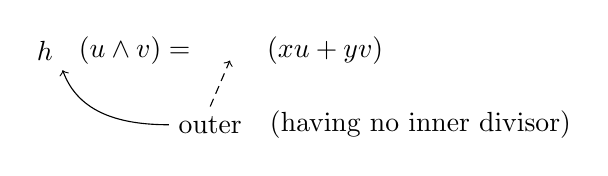
\begin{tikzpicture}[x=1cm,y=1cm]
\node (h) at (0,0) {\(h\)};
\node at (1.14,0) {\((u\wedge v)=\)};
\node (ink) at (2.35,0) {\(\square\)};
\node at (3.56,0) {\((xu+yv)\)};
\node (outer) at (2.1,-.94) {outer};
\node[anchor=west] at ([xshift=1.1mm]outer.east) {(having no inner divisor)};
\draw[->] (outer.west) to[out=180,in=290] (h.south east);
\draw[->,densely dashed] (outer.north) -- (ink.south);
\end{tikzpicture}}\endgroup\par}
\end{GelfandAdjacentEvidence}
\begin{GelfandAdjacentEvidence}{GELFAND-P000736}{6}

\Unclear{GELFAND-P000736}{overwritten-coefficient}{The sign before the parentheses is blacked out. The stroke directly below it is also heavily crossed out.}
\end{GelfandAdjacentEvidence}
\begin{GelfandAdjacentEvidence}{GELFAND-P000736}{7}

\Unclear{GELFAND-P000736}{margin-right-curve}{A broken curved stroke appears in the right margin. Its purpose is unclear.}
\end{GelfandAdjacentEvidence}
\begin{GelfandAdjacentEvidence}{GELFAND-P000736}{8}


\uwave{Fix an inner fn. \(\omega\).} Then \(\forall u,v\ \exists x,y\colon\)
\[
xu+yv=h_\omega(u\wedge v),\quad\text{where }h_\omega\wedge\omega=1
\]
(but \(h_\omega\) need not be outer)
\Unclear{GELFAND-P000736}{outer-word}{The last word tentatively reads “внешний” (outer). The middle letters are heavily retraced.}
\end{GelfandAdjacentEvidence}
\begin{GelfandAdjacentEvidence}{GELFAND-P000736}{9}


In fact, one can choose \(x,y=\mathrm{const}\)
\[
\text{\uwave{\(u+tv=h_t(u\wedge v)\)}}
\]
\uwave{M. Sherman} (beautiful proofs of the lemma)

\uwave{Generalization:}

[crossed out] \(\forall u_1,\ldots,u_r,\)
\Incomplete{GELFAND-P000736}{abandoned-before-quantifier}{The overwritten group before the quantifier is illegible.}
\end{GelfandAdjacentEvidence}
\begin{GelfandAdjacentEvidence}{GELFAND-P000736}{10}

\[
u_1+tu_2+\cdots+t^{r-1}u_{r+1}
=h_t\Bigl(\bigwedge_k u_k\Bigr);\quad h_t\wedge\omega=1
\]
\Unclear{GELFAND-P000736}{sequence-final-index}{The last subscript tentatively reads \(r+1\).}
\end{GelfandAdjacentEvidence}
\begin{GelfandAdjacentEvidence}{GELFAND-P000736}{11}

\Incomplete{GELFAND-P000736}{sequence-index-underink}{The earlier strokes beneath the heavy mark in the index are illegible.}
\end{GelfandAdjacentEvidence}
\begin{GelfandAdjacentEvidence}{GELFAND-P000736}{12}

(Except for a countable set of values of \(t\))

and likewise for a finite number of rows

Then some elementary matrix transformations.

\underline{\underline{I. Krichever.}}

\uwave{Rat. solutions of the Kadomtsev–Petviashvili equation:}
\begin{equation*}
\tag*{(1)\hfill}
\frac34 u_{yy}+\frac{\partial}{\partial x}
\left\{\text{[crossed out]}\frac{\partial u}{\partial t}
+\frac14(6uu_x+u_{xxx})\right\}=0
\end{equation*}
\Incomplete{GELFAND-P000736}{kp-cancel-before-time-derivative}{The crossed-out sign before the time derivative is illegible.}
\end{GelfandAdjacentEvidence}



\Needspace{7\baselineskip}
\begin{GelfandAdjacentEvidence}{GELFAND-P000737}{1}
\SourcePage{GELFAND-P000737}{78}
\underline{Theorem.} \uwave{Seek solns. rational in \(x\)} \(u(x,y,t)\),
\uwave{decaying as \(\lvert x\rvert\to\infty\).}
\uwave{Then} it is easy to see that
\Unclear{GELFAND-P000737}{easy-final-word}{The word before “see” reads “легко” (easy). Its last letter is heavily retraced.}
\end{GelfandAdjacentEvidence}
\begin{GelfandAdjacentEvidence}{GELFAND-P000737}{2}

\Incomplete{GELFAND-P000737}{easy-word-underink}{The earlier strokes of the last letter are illegible beneath the heavy retracing.}
\end{GelfandAdjacentEvidence}
\begin{GelfandAdjacentEvidence}{GELFAND-P000737}{3}

\[
u(x,y,t)=\sum\frac{-2}{\bigl(x-x_j(y,t)\bigr)^2}
\]
\Unclear{GELFAND-P000737}{pole-argument-y}{The lower loop identifies the first argument of \(x_j\) as \(y\).}
\end{GelfandAdjacentEvidence}
\begin{GelfandAdjacentEvidence}{GELFAND-P000737}{4}

\Incomplete{GELFAND-P000737}{pole-argument-underink}{The earlier strokes of the argument are illegible beneath the correction.}
\end{GelfandAdjacentEvidence}
\begin{GelfandAdjacentEvidence}{GELFAND-P000737}{5}


1) \uwave{The poles move in \(y\) acc. to Moser’s syst.} \uwave{with Hamiltonian}
\[
H=\frac12\sum p_j^2+\sum_{i<j}\frac{1}{(x_i-x_j)^2}
\]
(\(t\) \uwave{fixed})

2) \uwave{The poles move in \(t\)} [crossed out] \uwave{according to Hamiltonian \(F_3\), one of the integrals of Moser’s syst.}
\Incomplete{GELFAND-P000737}{cancel-after-time-motion}{The crossed-out mark after the abbreviation for “move” is illegible.}
\end{GelfandAdjacentEvidence}
\begin{GelfandAdjacentEvidence}{GELFAND-P000737}{6}


We obtain 2 commuting flows determining [inserted above: (rat.)] solns. of eq. (1).

\SourceFigure{GELFAND-P000737}{separator}{%
\par\begingroup\color{black}\GelfandFitDiagram{\begin{tikzpicture}[x=1cm,y=1cm]
\draw (0,0)--(1.15,0);
\fill (1.49,-.01) circle[radius=.022];
\draw (2.21,-.01)--(3.64,-.06);
\end{tikzpicture}}\endgroup\par}
\end{GelfandAdjacentEvidence}
\begin{GelfandAdjacentEvidence}{GELFAND-P000737}{7}


\[
(1)\Longleftrightarrow
\left[\frac{\partial}{\partial y}-L_1,\frac{\partial}{\partial t}-L_2\right]=0,
\]
\[
L_1=\frac{d^2}{dx^2}+u,\qquad
L_2=\frac{d^3}{dx^3}+\frac32u\frac{d}{dx}+u
\]
\Incomplete{GELFAND-P000737}{l2-coefficient-underink}{The coefficient reads \(3/2\). The earlier strokes under the heavy retracing are illegible.}
\end{GelfandAdjacentEvidence}
\begin{GelfandAdjacentEvidence}{GELFAND-P000737}{8}

\Unclear{GELFAND-P000737}{l2-final-term}{The final term is written \(+u\).}
\end{GelfandAdjacentEvidence}
\begin{GelfandAdjacentEvidence}{GELFAND-P000737}{9}


We obtain commutative subalgebras in \(\mathcal D_n\) (division ring of fractions of the ring of diff. ops. with polyn. coeffs. in \(n\) variables)

Next time \underline{Yu. I. Manin}
\Unclear{GELFAND-P000737}{bibliography-abbreviation}{The faint abbreviation before “раз” (time) tentatively reads “След.” (next).}
\end{GelfandAdjacentEvidence}



\clearpage\pdfbookmark[0]{Chapter 12}{gelfand-archive-chapter-12}
\section*{Chapter 12}


\Needspace{7\baselineskip}
\begin{GelfandAdjacentEvidence}{GELFAND-P000738}{1}
\SourcePage{GELFAND-P000738}{6}
\noindent\underline{\underline{21/\(\overline{\underline{\mathrm{XI}}}\)-77.}}\qquad
\underline{\underline{Gelfand Sem.}}

\SourceFigure{GELFAND-P000738}{speaker-box}{%
\par{\setlength{\fboxsep}{3pt}\fcolorbox{red}{white}{\underline{\textbf{Yu. I. Manin.}}}}\par}
\end{GelfandAdjacentEvidence}
\begin{GelfandAdjacentEvidence}{GELFAND-P000738}{2}


(on work with \uwave{V. Drinfeld})

\underline{Description of self-dual solutions of the Yang–Mills eqs.}

\(\mathbb R^4\ni(x_1,x_2,x_3,x_4)\). \qquad Unknown functions:

\[
A_\mu(x)\in u(r),\qquad r\geq 2
\]
(Hermitian or anti-Hermitian matrices; in the Lie algebra)
\SourceFigure{GELFAND-P000738}{algebra-pointer}{%
\par\begingroup\color{black}\GelfandFitDiagram{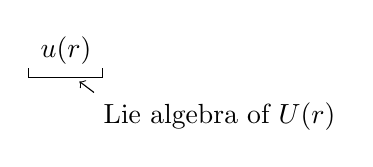
\begin{tikzpicture}[x=1cm,y=1cm]
\node (algebra) at (0,0) {\(u(r)\)};
\draw (-.48,-.22)--(-.48,-.34)--(.46,-.34)--(.46,-.22);
\node (label) at (1.95,-.83) [align=left] {Lie algebra of \(U(r)\)};
\draw[->] (label.north west)--(.17,-.39);
\end{tikzpicture}}\endgroup\par}
\end{GelfandAdjacentEvidence}
\begin{GelfandAdjacentEvidence}{GELFAND-P000738}{3}

\(u(r)\) --- the set of skew-Hermitian \(r\times r\) matrices.

\begin{equation*}
\tag*{(1)\hfill}
F_{\mu\nu}(x)\underset{\mathrm{def}}{=}
\frac{\partial}{\partial x_\mu}A_\nu
-\frac{\partial}{\partial x_\nu}A_\mu+[A_\mu,A_\nu]
\end{equation*}

1) \uwave{Duality equations:}

\(\rho\sigma\) --- complementary pair of indices to \(\mu\nu\), \quad \(F_{\mu\nu}=\pm F_{\rho\sigma}\); more precisely:
\begin{equation*}
\tag*{(2)\hfill}
F_{\mu\nu}=\varepsilon^{\mu\nu\rho\sigma}F_{\rho\sigma}
\end{equation*}
(\(\varepsilon^{\mu\nu\rho\sigma}\) --- the sign of the permutation).

2) \uwave{Regularity conditions:} \quad A) at finite points \quad B) at infinity

A) singularities at finite points can be removed by a gauge transformation.

More precisely, consid. the bundle \(\mathbb C^r\times\mathbb R^4\) and a basis of sections in it;
the covariant differential, determined by the matrices \(A_\mu\), is given by the formula:
\begin{equation*}
\tag*{(3)\hfill}
\partial_\mu\begin{pmatrix}s_1\\ \vdots\\ s_r\end{pmatrix}
=A_\mu\begin{pmatrix}s_1\\ \vdots\\ s_r\end{pmatrix},
\qquad
\partial_\mu s_i=\sum_{i=1}^{r}A_\mu^{ij}s_j.
\end{equation*}
\Unclear{GELFAND-P000738}{eq-03-summation}{The lower limit of summation reads \(i=1\). The \(i\) in \(s_i\) on the left is heavily retraced.}
\end{GelfandAdjacentEvidence}
\begin{GelfandAdjacentEvidence}{GELFAND-P000738}{4}

\SourceFigure{GELFAND-P000738}{section-pointer}{%
\par\begingroup\color{black}\GelfandFitDiagram{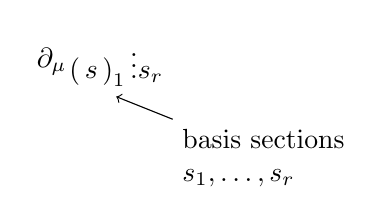
\begin{tikzpicture}[x=1cm,y=1cm]
\node at (0,0) {\(\partial_\mu\)};
\node (sections) at (.82,0) {\(\begin{pmatrix}s_1\\ \vdots\\ s_r\end{pmatrix}\)};
\node (basis) at (2.69,-1.22) [align=left] {basis sections\\ \(s_1,\ldots,s_r\)};
\draw[->] (basis.north west)--(sections.south);
\end{tikzpicture}}\endgroup\par}
\end{GelfandAdjacentEvidence}
\begin{GelfandAdjacentEvidence}{GELFAND-P000738}{5}


Pass to another basis. We obtain a transformation (gauge transformation).
\begin{equation*}
\tag*{(4)\hfill}
A_\mu\mapsto u^{-1}\partial_\mu u+u^{-1}A_\mu u=A'_\mu
\end{equation*}

\uwave{Regularity condition at a finite point:} there is a genuine connection without singularities, i.e. the sing. in \(A_\mu\) can be removed by a gauge transformation.

Transition:
\SourceFigure{GELFAND-P000738}{basis-change}{%
\par\begingroup\color{black}\GelfandFitDiagram{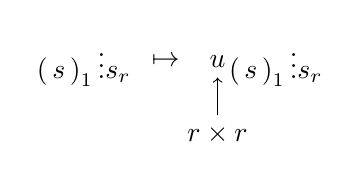
\begin{tikzpicture}[x=1cm,y=1cm]
\node at (0,0) {\(\begin{pmatrix}s_1\\ \vdots\\ s_r\end{pmatrix}\)};
\node at (1.04,0) {\(\mapsto\)};
\node (change) at (1.70,0) {\(u\)};
\node at (2.44,0) {\(\begin{pmatrix}s_1\\ \vdots\\ s_r\end{pmatrix}\)};
\node (size) at (1.70,-.92) {\(r\times r\)};
\draw[->] (size.north)--(change.south);
\end{tikzpicture}}\endgroup\par}
\end{GelfandAdjacentEvidence}
\begin{GelfandAdjacentEvidence}{GELFAND-P000738}{6}


B) \uwave{Conditions at} \(P=\infty\).

The bundle on
\(\mathbb R^4\) extends to a bund. over \(S^4=\mathbb R^4\cup\{\infty\}\).
\SourceFigure{GELFAND-P000738}{bundle-projection}{%
\par\begingroup\color{black}\GelfandFitDiagram{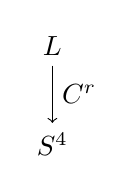
\begin{tikzpicture}[x=1cm,y=1cm]
\node (bundle) at (0,0) {\(L\)};
\node (sphere) at (0,-1.24) {\(S^4\)};
\draw[->] (bundle)--node[right]{\(\mathbb C^r\)}(sphere);
\end{tikzpicture}}\endgroup\par}
\end{GelfandAdjacentEvidence}

\(L\) --- the space of our bundle.

\uwave{Regularity cond.:} The connection \(\partial_\mu\) extends to a connection in \(L\) over \(S^4\)
(the bundle \(L\) need no longer be trivial)


\Needspace{7\baselineskip}
\begin{GelfandAdjacentEvidence}{GELFAND-P000739}{1}
\SourcePage{GELFAND-P000739}{unlabelled}
This also means that a twist at infinity can remove the singularity.

An essential invariant of the solution is the bundle \(L\). This is a discrete invariant. On \(L\) there is a unitary bundle structure.

\uwave{Classification of} \(L\).

Gluing the trivializations on the equator gives a map \(S^3\to U(r)\), i.e. an element of \(\pi_3(U(r))=\mathbb Z\).

(\(SU(2)\subset U(r)\), \(SU(2)\cong S^3\); hence an integer-valued sufficient invariant
\(=\) degree of the map \(n\) \(=\) Pontryagin number)
\Unclear{GELFAND-P000739}{integer-invariant}{The word after “integer-valued” reads “достаточный” (sufficient). Its first letters are heavily retraced.}
\end{GelfandAdjacentEvidence}
\begin{GelfandAdjacentEvidence}{GELFAND-P000739}{2}


the embedding \(SU(2)\subset U(r)\) is taken in the form
\SourceFigure{GELFAND-P000739}{block-embedding}{%
\par\begingroup\color{black}\GelfandFitDiagram{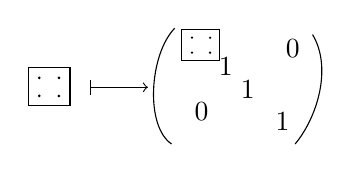
\begin{tikzpicture}[x=1cm,y=1cm]
\draw (0,0) rectangle (.53,.48);
\foreach \x in {.14,.39} \foreach \y in {.12,.35} {\fill (\x,\y) circle[radius=.019];}
\draw[|->] (.78,.23)--(1.52,.23);
\draw (1.86,.98) .. controls (1.54,.65) and (1.48,-.26) .. (1.82,-.49);
\draw (3.61,.90) .. controls (3.86,.49) and (3.68,-.14) .. (3.39,-.49);
\draw (1.95,.57) rectangle (2.43,.96);
\foreach \x in {2.08,2.31} \foreach \y in {.67,.86} {\fill (\x,\y) circle[radius=.016];}
\node at (2.51,.49) {\(1\)};
\node at (2.79,.20) {\(1\)};
\node at (3.23,-.20) {\(1\)};
\node at (3.36,.72) {\(0\)};
\node at (2.20,-.08) {\(0\)};
\end{tikzpicture}}\endgroup\par}
\end{GelfandAdjacentEvidence}
\begin{GelfandAdjacentEvidence}{GELFAND-P000739}{3}


\uwave{We shall assume} \(n\geq0\) and the duality conditions

(\(n<0\ \Rightarrow\) we can change the sign in eq. (2))\\
\hspace*{2em}--- anti-self-dual solns. --- reduce to \(n>0\))
\Unclear{GELFAND-P000739}{extra-parenthesis}{Closing parentheses are visible after “(2)” and at the end of the following line.}
\end{GelfandAdjacentEvidence}
\begin{GelfandAdjacentEvidence}{GELFAND-P000739}{4}


\uwave{Plan for what follows:}

[Crossed-out line]
\Incomplete{GELFAND-P000739}{plan-deleted-line}{The line below the heading is heavily crossed out and illegible.}
\end{GelfandAdjacentEvidence}
\begin{GelfandAdjacentEvidence}{GELFAND-P000739}{5}


\SourceFigure{GELFAND-P000739}{diagram-plan}{%
\par\begingroup\color{black}\GelfandFitDiagram{\begin{tikzpicture}[x=.82cm,y=.85cm,font=\small]
\node (start) at (0,0) {\(\left(\begin{gathered}L\\\downarrow\\S^4\end{gathered},\,A_\mu\right)\)};
\draw[->] plot[smooth] coordinates {(1.0,0) (1.15,.07) (1.29,-.045) (1.45,.07) (1.61,-.04) (1.79,.03) (2.08,.015)};
\draw (2.60,.54)--(2.40,.54)--(2.40,-2.57)--(2.60,-2.57);
\node (trivial) at (3.39,.47) {\(H\times S^4\)};
\node (base) at (3.40,-.61) {\(S^4\)};
\draw[->] (trivial.south)--(base.north);
\node (rank) at (3.88,1.32) {\(2n+r\)};
\draw[->] (rank.south west)--(trivial.north west);
\node at (6.39,.14) {\(H=\mathbb C^{2n+r}\),};
\node[anchor=west,align=left] at (2.53,-1.68) {Here:\\{[crossed out]}\\Hermitian metric\\trivial connection};
\draw[->] (1.99,-1.64)--(.82,-.66);
\node (orthogonal) at (.18,-3.55) [align=left] {Explicitly constructed\\decomp. into orthog. parts};
\draw[->] (orthogonal.north)--(1.19,-1.18);
\end{tikzpicture}}\endgroup\par}
\end{GelfandAdjacentEvidence}
\begin{GelfandAdjacentEvidence}{GELFAND-P000739}{6}

\Incomplete{GELFAND-P000739}{diagram-deleted-caption}{A short phrase is crossed out inside the large bracket. The first letter resembles Cyrillic “с”.}
\end{GelfandAdjacentEvidence}
\begin{GelfandAdjacentEvidence}{GELFAND-P000739}{7}


\SourceFigure{GELFAND-P000739}{rank-decomposition}{%
\par\begingroup\color{black}\(\begin{array}{lccccc}
\text{Dimensions:}&2n+r&&r&&2n\\
&\downarrow&&\downarrow&&\downarrow\\
\text{Decomposition:}&H\times S^4&=&L&\oplus&L^\perp
\end{array}\)\endgroup\par}
\end{GelfandAdjacentEvidence}
\begin{GelfandAdjacentEvidence}{GELFAND-P000739}{8}


\(\{A_\mu\}\) --- a direct summand of the trivial connection in \(H\times S^4\)

(Differentiate and project onto \(L\)).

Unitarity of the connection is proved.

[This generalizes the fact that a Riemannian space can be embedded in Euclidean space; can we [inserted above: always] embed a bundle with connection?]
\Unclear{GELFAND-P000739}{riemannian-space}{The abbreviation after “Riemannian” reads “пр-во” (space).}
\end{GelfandAdjacentEvidence}
\begin{GelfandAdjacentEvidence}{GELFAND-P000739}{9}


Which decompositions give self-dual fields?

We must pass from the base \(S^4\) to its \uwave{complexification}.

In \(\mathbb C^4\) consider the map
\[
\sigma:\ z\mapsto(-\overline z_2,\overline z_1,-\overline z_4,\overline z_3).
\]
\SourceFigure{GELFAND-P000739}{coordinate-pointer}{%
\par\begingroup\color{black}\GelfandFitDiagram{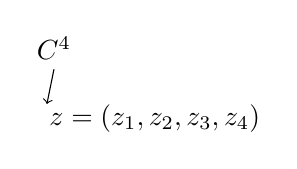
\begin{tikzpicture}[x=1cm,y=1cm]
\node (space) at (0,.89) {\(\mathbb C^4\)};
\node at (1.28,0) {\(z=(z_1,z_2,z_3,z_4)\)};
\draw[->] (space.south)--(-.09,.18);
\end{tikzpicture}}\endgroup\par}
\end{GelfandAdjacentEvidence}

(in quaternions, multiplication by \(i\))

For \(\sigma\) there are no fixed pts. (\(\text{except }0\)) and no fixed lines, but there are invariant planes
\begin{equation*}
\tag*{(5)\hfill}
\mathbb C z+\mathbb C\sigma(z)\subset\mathbb C^4
\end{equation*}


\Needspace{7\baselineskip}
\begin{GelfandAdjacentEvidence}{GELFAND-P000740}{1}
\SourcePage{GELFAND-P000740}{7}
We shall call them \uwave{real} (or \uwave{\(\sigma\)-invariant})
(\(\sigma\) --- involution).

\begin{equation*}
\tag*{(6)\hfill}
\{\sigma\text{-invar. planes}\}=S^4
\end{equation*}
(\uwave{proof omitted})

(in \(\mathbb C P^3\) this is the set of \(\sigma\)-invar. lines).

\(E^4\subset\) [crossed out] \(S^4=E^4\cup\{\infty\}\).
\Incomplete{GELFAND-P000740}{compactification-cancel}{A mark between the inclusion sign and \(S^4\) is heavily crossed out.}
\end{GelfandAdjacentEvidence}
\begin{GelfandAdjacentEvidence}{GELFAND-P000740}{2}


Hence there is a map
\begin{equation*}
\tag*{(7)\hfill}
\mathbb C^4\setminus\{0\}\overset{D}{\longrightarrow}S^4\supset E^4.
\end{equation*}
\[
z\longmapsto \sigma\text{-invar. plane through }z.
\]
Write \(D\) in coordinates (\(\text{in } E^4\) the coordinates are \((x_i)\)).
The normalization is as in Zakharov–Belavin.

\[
(z_1,z_2,z_3,z_4)\longmapsto
\begin{cases}
x_2+i x_1=\dfrac{z_1\bar z_3+\bar z_2 z_4}{|z_3|^2+|z_4|^2},\\[6pt]
x_4+i x_3=\dfrac{\bar z_2 z_3-z_1\bar z_4}{|z_3|^2+|z_4|^2}.
\end{cases}
\]
(Plücker coordinates of the [inserted above: \(\sigma\)-inv.] plane through pt. \(z\))
\Unclear{GELFAND-P000740}{plane-insertion}{The abbreviation “\(\sigma\)-инв.” is inserted above the line with a mark indicating its position.}
\end{GelfandAdjacentEvidence}
\begin{GelfandAdjacentEvidence}{GELFAND-P000740}{3}


This is the map
\[
\mathbb C^4\setminus\{z_3=z_4=0\}\longrightarrow E^4.
\]
\underline{Remark:} to recover a \(\sigma\)-inv. plane, 3 coordinates suffice.

\underline{\underline{Lemma 1}}
\(\bigl(\overset{4}{\text{A}}\,
\overset{2}{\text{W}}\,
\overset{1?}{\text{B}}\,
\overset{3}{\text{Z}}\bigr.\)
--- Atiyah, Ward, Belavin, Zakharov).
\Unclear{GELFAND-P000740}{attribution-numeral}{Above “Б” is a heavy vertical mark, tentatively 1. The other numbers read 4, 2 and 3.}
\end{GelfandAdjacentEvidence}
\begin{GelfandAdjacentEvidence}{GELFAND-P000740}{4}

\Unclear{GELFAND-P000740}{belavin-correction}{The beginning of “Belavin” is heavily retraced.}
\end{GelfandAdjacentEvidence}
\begin{GelfandAdjacentEvidence}{GELFAND-P000740}{5}


a)
\[
D^*(dx_\mu\wedge dx_\nu+\varepsilon^{\mu\nu\rho\sigma}dx_\rho\wedge dx_\sigma)
\quad\text{--- a form of type }(1,1).
\]
(Consider such forms and lift them to \(\mathbb C^4\setminus0\) using \(D\))

b)
\[
\left[D^*\left(\begin{array}{l}
dx_1\wedge dx_2,\\
dx_1\wedge dx_3,\\
dx_1\wedge dx_4
\end{array}\right)\right]^{2,0}
\qquad\text{linearly independent.}
\]
[crossed out]
\Incomplete{GELFAND-P000740}{independence-cancel}{A short fragment after “linearly independent” is heavily crossed out.}
\end{GelfandAdjacentEvidence}
\begin{GelfandAdjacentEvidence}{GELFAND-P000740}{6}


\((2,0)\)-components.

\underline{Corollary 1} (AW).

\begin{equation*}
\tag*{(8)\hfill}
\left[D^*\left(\sum F_{\mu\nu}\,dx_\mu\wedge dx_\nu\right)\right]=0
\quad\Longleftrightarrow\quad
F_{\mu\nu}=\varepsilon^{\mu\nu\rho\sigma}F_{\rho\sigma}.
\end{equation*}
\Unclear{GELFAND-P000740}{corollary-projection}{The closing square bracket in (8) has no written component index.}
\end{GelfandAdjacentEvidence}



\Needspace{7\baselineskip}
\begin{GelfandAdjacentEvidence}{GELFAND-P000741}{1}
\SourcePage{GELFAND-P000741}{unlabelled}
\underline{Corollary \(1'\)} (BZ)

\SourceFigure{GELFAND-P000741}{derivative-annotations}{%
\par\begingroup\color{black}\GelfandFitDiagram{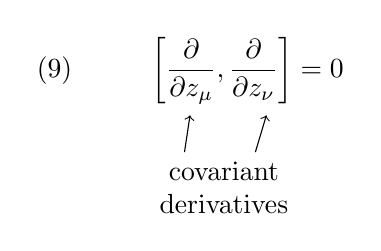
\begin{tikzpicture}[x=1cm,y=1cm]
\node at (-.70,0) {\((9)\)};
\node at (1.75,0) {\(\displaystyle\left[\frac{\partial}{\partial z_\mu},
  \frac{\partial}{\partial z_\nu}\right]=0\)};
\node (covariant) at (1.45,-1.49) [align=center] {covariant\\derivatives};
\draw[->] ([xshift=-5mm]covariant.north)--(1.02,-.57);
\draw[->] ([xshift=4mm]covariant.north)--(1.99,-.57);
\end{tikzpicture}}\endgroup\par}
\end{GelfandAdjacentEvidence}
\begin{GelfandAdjacentEvidence}{GELFAND-P000741}{2}

\Unclear{GELFAND-P000741}{covariant-ending}{The ending of the Russian word for “covariant” is heavily retraced.}
\end{GelfandAdjacentEvidence}
\begin{GelfandAdjacentEvidence}{GELFAND-P000741}{3}


\underline{\underline{Belavin.}} Or:
\begin{equation*}
\tag{10}
[\nabla_\mu,\nabla_\nu]=0,
\end{equation*}
where
\begin{equation*}
\tag{11}
\nabla_\mu=\frac{\partial}{\partial z_\mu}+C_\mu,
\end{equation*}
\begin{equation*}
\tag{12}
\left[D^*\left(\sum A_\mu\,dx_\mu\right)\right]^{1,0}=\sum C_a\,dz_a
\end{equation*}
\Unclear{GELFAND-P000741}{equation-number}{The digit 2 in equation number (12) is heavily retraced.}
\end{GelfandAdjacentEvidence}
\begin{GelfandAdjacentEvidence}{GELFAND-P000741}{4}

\Unclear{GELFAND-P000741}{form-index}{The indices on the right of (12) tentatively read \(a\), possibly \(\alpha\).}
\end{GelfandAdjacentEvidence}
\begin{GelfandAdjacentEvidence}{GELFAND-P000741}{5}


Or: set
\begin{equation*}
\tag{13}
C_i(z)=\frac{\partial x_\mu}{\partial z_i}A_\mu(x)
\end{equation*}
\Unclear{GELFAND-P000741}{coordinate-retraced}{The \(z\) in the denominator of (13) is heavily retraced.}
\end{GelfandAdjacentEvidence}
\begin{GelfandAdjacentEvidence}{GELFAND-P000741}{6}


Then
\begin{equation*}
\tag{14}
\text{[crossed out]}\quad
\frac{\partial C_k}{\partial z_i}-\frac{\partial C_i}{\partial z_k}+[C_i,C_k]=0
\end{equation*}
\Incomplete{GELFAND-P000741}{equation14-cancel}{The first sign of the crossed-out group resembles \(\partial\). The other signs are illegible.}
\end{GelfandAdjacentEvidence}
\begin{GelfandAdjacentEvidence}{GELFAND-P000741}{7}

by virtue of the duality equations.

Or:
\begin{equation*}
\tag{15}
[L_1,L_2]=0,
\end{equation*}
where
\begin{equation*}
\tag{\(16'\)}
L_1=\lambda(\nabla_1-i\nabla_2)+(\nabla_3+i\nabla_4),
\end{equation*}
\Unclear{GELFAND-P000741}{lax-i-retraced}{The sign after the minus in (16′) is heavily retraced and tentatively reads \(i\).}
\end{GelfandAdjacentEvidence}
\begin{GelfandAdjacentEvidence}{GELFAND-P000741}{8}

\begin{equation*}
\tag{\(16''\)}
L_2=\lambda(\nabla_3-i\nabla_4)-(\nabla_1+i\nabla_2),
\end{equation*}
\Unclear{GELFAND-P000741}{lax-sign}{Between the parentheses in (16″) there is a heavy horizontal stroke and short vertical traces. It is tentatively read as a minus.}
\end{GelfandAdjacentEvidence}
\begin{GelfandAdjacentEvidence}{GELFAND-P000741}{9}

\begin{equation*}
\tag{17}
\nabla_\mu\equiv\partial_\mu+A_\mu
\end{equation*}

\underline{\underline{M.}} \underline{Construction of bundles.} They will be constructed on the left.
\SourceFigure{GELFAND-P000741}{bundle-diagram}{%
\par\begingroup\color{black}\GelfandFitDiagram{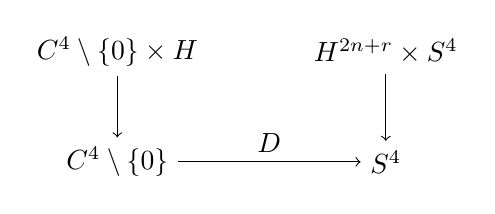
\begin{tikzpicture}[x=1cm,y=1cm]
\node (left) at (0,0) {\(\mathbb C^4\setminus\{0\}\times H\)};
\node (right) at (3.41,0) {\(H^{2n+r}\times S^4\)};
\node (leftbase) at (0,-1.40) {\(\mathbb C^4\setminus\{0\}\)};
\node (rightbase) at (3.41,-1.40) {\(S^4\)};
\draw[->] (left)--(leftbase);
\draw[->] (right)--(rightbase);
\draw[->] (leftbase)--node[above]{\(D\)}(rightbase);
\end{tikzpicture}}\endgroup\par}
\end{GelfandAdjacentEvidence}
\begin{GelfandAdjacentEvidence}{GELFAND-P000741}{10}


\uwave{Objects of linear algebra} \(\Rightarrow\) direct summand in \(H\times S^4\).

\(H\) --- \((2n+r)\)-dimensional Hermitian space,\\
\hspace*{2em}form \(Q\).

Consider [crossed out]
\begin{equation*}
\tag{18}
I\subset H\otimes_{\mathbb C}\mathbb C^4\qquad(*)
\end{equation*}
\Incomplete{GELFAND-P000741}{object-mark}{A separate small crossed-out mark appears before (18).}
\end{GelfandAdjacentEvidence}
\begin{GelfandAdjacentEvidence}{GELFAND-P000741}{11}

\(I\) --- \(n\)-dimensional subspace

\SourceFigure{GELFAND-P000741}{object-bracket}{%
\par\begingroup\color{black}\GelfandFitDiagram{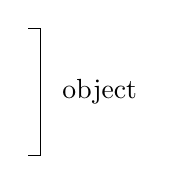
\begin{tikzpicture}[x=1cm,y=1cm]
\draw (0,.81)--(.16,.81)--(.16,-.81)--(0,-.81);
\node[anchor=west] at (.31,0) {\uwave{object}};
\end{tikzpicture}}\endgroup\par
The right bracket covers the passage from the definition of \(H\) to the line about the subspace \(I\).}
\end{GelfandAdjacentEvidence}



\Needspace{7\baselineskip}
\begin{GelfandAdjacentEvidence}{GELFAND-P000742}{1}
\SourcePage{GELFAND-P000742}{8}
\uwave{Conditions.}

From the object we construct something like a bundle.

\(L(*)=\) “system of linear spaces over \(S^4\)”.

\SourceFigure{GELFAND-P000742}{plane-description}{%
\par\begingroup\color{black}\GelfandFitDiagram{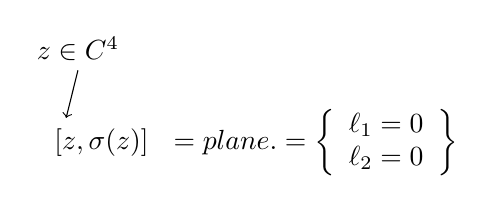
\begin{tikzpicture}[x=1cm,y=1cm]
\node (vector) at (-.30,1.19) {\(z\in\mathbb C^4\)};
\node (plane) at (0,0) {\([z,\sigma(z)]\)};
\draw[->] (vector.south)--(-.45,.31);
\node[anchor=west] at (.79,0) {\(=\text{plane.}=\left\{\begin{array}{l}
\ell_1=0\\ \ell_2=0
\end{array}\right\}\)};
\end{tikzpicture}}\endgroup\par}
\end{GelfandAdjacentEvidence}
\begin{GelfandAdjacentEvidence}{GELFAND-P000742}{2}

\(\ell_{1,2}:\mathbb C^4\to\mathbb C\) --- linear forms.

\SourceFigure{GELFAND-P000742}{image-diagram}{%
\par\begingroup\color{black}\GelfandFitDiagram{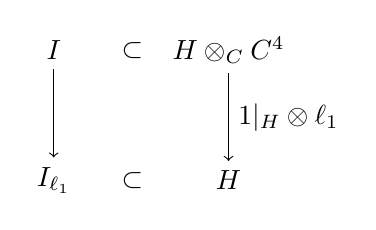
\begin{tikzpicture}[x=1cm,y=1cm]
\node (i) at (0,0) {\(I\)};
\node at (1,0) {\(\subset\)};
\node (tensor) at (2.22,0) {\(H\otimes_{\mathbb C}\mathbb C^4\)};
\node (image) at (0,-1.65) {\(I_{\ell_1}\)};
\node at (1,-1.65) {\(\subset\)};
\node (h) at (2.22,-1.65) {\(H\)};
\draw[->] (i)--(image);
\draw[->] (tensor)--node[right]{\(1|_H\otimes\ell_1\)}node[left]{\(\square\)}(h);
\end{tikzpicture}}\endgroup\par}
\end{GelfandAdjacentEvidence}
\begin{GelfandAdjacentEvidence}{GELFAND-P000742}{3}

\Incomplete{GELFAND-P000742}{image-diagram-mark}{The heavily retraced mark to the left of the right-hand arrow is illegible.}
\end{GelfandAdjacentEvidence}
\begin{GelfandAdjacentEvidence}{GELFAND-P000742}{4}

\Unclear{GELFAND-P000742}{identity-subscript}{To the right of the arrow the label reads \(1|_H\otimes\ell_1\).}
\end{GelfandAdjacentEvidence}
\begin{GelfandAdjacentEvidence}{GELFAND-P000742}{5}


Construct analogously \(I_{\ell_2}\).

Thus we have constructed 2 subspaces \(I_{\ell_1},I_{\ell_2}\subset H\)

It turns out that
\[
I_{\ell_1}+I_{\ell_2}\quad \text{[crossed out: depends?]}
\]
\Unclear{GELFAND-P000742}{dependence-cancel}{The crossed-out word to the right of the sum tentatively reads “зависит” (depends).}
\end{GelfandAdjacentEvidence}
\begin{GelfandAdjacentEvidence}{GELFAND-P000742}{6}

depends only on the \(\sigma\)-invar. plane \([z,\sigma(z)]\), i.e. a point of \(S^4\)
\[
(I_{\ell_1}+I_{\ell_2})^\perp
=\text{lin. subspace in }H,\ \text{corresponding to }[z,\sigma(z)].
\]

\uwave{Condition 1.} A bundle must result
(the dimensions are maximal, i.e. the right ones), namely
\begin{equation*}
\tag{19}
\dim(I_{\ell_1}+I_{\ell_2})^\perp=r
\end{equation*}

\uwave{Condition} 2. Hermitian property of the bundle.

The form \(Q|_{I_{\ell_1}+I_{\ell_2}}>0\)

(a priori \(Q\) is not assumed to be \(>0\), but it turns out to do so under this condition).

A direct summand results. The connection is obtained by projecting the trivial one.

\underline{Theorem 1.} \uwave{This gives all} [inserted above: \uwave{self-dual}]
\uwave{solutions of the Y.–M. equation}, \uwave{nonisom. bunds. correspond to inequivalent solutions}.
\Unclear{GELFAND-P000742}{self-dual-insertion}{“Self-dual” is inserted above “solutions” and wavy-underlined.}
\end{GelfandAdjacentEvidence}


One more condition has been omitted.

Take the eqs.:
\[
\left\{\begin{array}{l}
\ell(z)=0\\
\ell(\sigma z)=0
\end{array}\right\}
\]


\Needspace{7\baselineskip}
\begin{GelfandAdjacentEvidence}{GELFAND-P000743}{1}
\SourcePage{GELFAND-P000743}{unlabelled}
\underline{Condition} 0.

\begin{equation*}
\tag{20}
Q(I_\ell,I_{\ell\circ\sigma})=0
\end{equation*}
\uwave{i.e.} \(I_\ell\) and \(I_{\ell\circ\sigma}\) \uwave{are orthogonal}.

This gives a problem in linear algebra.

\underline{\underline{G.}} it is contained in an unpubl. work of Gelfand and Ponomarev on quadruples with an automorphism.

\underline{Ponomarev:}
\[
I\hookrightarrow H\oplus H\oplus H\oplus H\longrightarrow A\longrightarrow 0
\]
\Unclear{GELFAND-P000743}{sequence-inclusion}{The first inclusion has an arrowhead. The first direct-sum sign is heavily retraced.}
\end{GelfandAdjacentEvidence}
\begin{GelfandAdjacentEvidence}{GELFAND-P000743}{2}

The images of the components \(H\) in \(A\) give 4 subspaces.

The complex invariants of the quadruple have been described.

Hermitian property: classify the quadruples invariant under the operation \(\perp\)
\Unclear{GELFAND-P000743}{orthogonal-abbreviation}{The abbreviation before “operation” tentatively reads “отн.” (with respect to). The middle strokes are heavily retraced.}
\end{GelfandAdjacentEvidence}
\begin{GelfandAdjacentEvidence}{GELFAND-P000743}{3}


a) Lagrangian subspaces, etc.

\SourceFigure{GELFAND-P000743}{paragraph-divider}{%
\par\begingroup\color{black}\GelfandFitDiagram{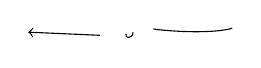
\begin{tikzpicture}[x=1cm,y=1cm]
\draw[<-] (0,.04)--(.91,0);
\draw (1.24,.02) .. controls (1.22,-.045) and (1.33,-.048) .. (1.33,.04);
\draw (1.59,.08) .. controls (1.93,.035) and (2.40,.03) .. (2.59,.09);
\end{tikzpicture}}\endgroup\par}
\end{GelfandAdjacentEvidence}
\begin{GelfandAdjacentEvidence}{GELFAND-P000743}{4}


M. \uwave{Turning all this into numbers.}

\SourceFigure{GELFAND-P000743}{parameter-bracket}{%
\par\begingroup\color{black}\GelfandFitDiagram{
\begin{tikzpicture}[x=1cm,y=1cm]
\node[inner sep=4pt] (i) {\(I\subset H\otimes\mathbb C^4\)};
\draw (i.north west)--(i.south west)--(i.south east)--(i.north east);
\end{tikzpicture}}\endgroup\par}
\end{GelfandAdjacentEvidence}
\begin{GelfandAdjacentEvidence}{GELFAND-P000743}{5}

--- parameters of a multi-instanton solution

isomorphism of diagrams gives identical solutions.

\SourceFigure{GELFAND-P000743}{diagram-isomorphism}{%
\par\begingroup\color{black}\GelfandFitDiagram{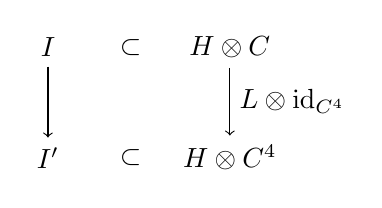
\begin{tikzpicture}[x=1cm,y=1cm]
\node (i) at (0,0) {\(I\)};
\node at (1.05,0) {\(\subset\)};
\node (top) at (2.31,0) {\(H\otimes\mathbb C\)};
\node (j) at (0,-1.40) {\(I'\)};
\node at (1.05,-1.40) {\(\subset\)};
\node (bottom) at (2.31,-1.40) {\(H\otimes\mathbb C^4\)};
\draw[->] (i)--(j);
\draw[->] (top)--node[right]{\(L\otimes\mathrm{id}_{\mathbb C^4}\)}(bottom);
\end{tikzpicture}}\endgroup\par}
\end{GelfandAdjacentEvidence}
\begin{GelfandAdjacentEvidence}{GELFAND-P000743}{6}

\Unclear{GELFAND-P000743}{diagram-upper-space}{The upper row reads \(H\otimes\mathbb C\), the lower row \(H\otimes\mathbb C^4\).}
\end{GelfandAdjacentEvidence}
\begin{GelfandAdjacentEvidence}{GELFAND-P000743}{7}


such isomorphisms of diagrams are allowed

\(L\) preserves the Hermitian form.

\uwave{Scheme for computing} \(A_\mu(x)\).

\begin{gather*}
(I\subset H\otimes\mathbb C^4,\quad e_1,\ldots,e_r\ \text{--- a basis of } I)
\longmapsto 4n\ \text{vectors in }H\\
(e_{ij}),\quad i=1,\ldots,n;\quad j=1,\ldots,4.\\
\dim H=2n+r.
\end{gather*}
\Unclear{GELFAND-P000743}{basis-terminal-index}{The last subscript in the list of basis vectors tentatively reads \(r\).}
\end{GelfandAdjacentEvidence}
\begin{GelfandAdjacentEvidence}{GELFAND-P000743}{8}


From them construct the matrix \(\widetilde Q\)

of \((n\times n)\) blocks of size \(4\times4\)

\((k\ell)\)-th block at position \((rs)\) has
\[
\underset{\text{numerical matrix}}{Q(e_{kr},e_{\ell s})}
\]
\Unclear{GELFAND-P000743}{form-first-index}{The second index of the first argument is heavily retraced. The reading is tentatively \(e_{kr}\).}
\end{GelfandAdjacentEvidence}


The matrix \(\widetilde Q\) determines the whole situation

\uwave{Assumption}: \(\operatorname{rk}\widetilde Q=2n+r\)
(\(\Leftrightarrow L\) has no nontrivial horizontal sections)
--- we omit such degeneracies for simplicity.


\Needspace{7\baselineskip}
\begin{GelfandAdjacentEvidence}{GELFAND-P000744}{1}
\SourcePage{GELFAND-P000744}{9}

\uwave{Which \(\widetilde Q\) are obtained:}

a) \(\widetilde Q\) is Hermitian;

b) \(\operatorname{rk}\widetilde Q=2n+r\);

c) “Condition 0”. This is a condition on all \(4\times4\) blocks

\SourceFigure{GELFAND-P000744}{block-matrix}{%
\par\begingroup\color{black}\GelfandFitDiagram{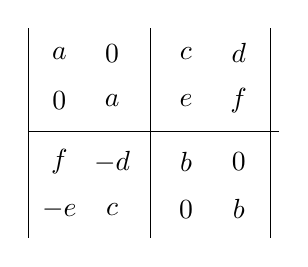
\begin{tikzpicture}[x=.67cm,y=.60cm]
\node at (0,0) {\(a\)}; \node at (1,0) {\(0\)};
\node at (2.4,0) {\(c\)}; \node at (3.4,0) {\(d\)};
\node at (0,-1) {\(0\)}; \node at (1,-1) {\(a\)};
\node at (2.4,-1) {\(e\)}; \node at (3.4,-1) {\(f\)};
\node at (0,-2.3) {\(f\)}; \node at (1,-2.3) {\(-d\)};
\node at (2.4,-2.3) {\(b\)}; \node at (3.4,-2.3) {\(0\)};
\node at (0,-3.3) {\(-e\)}; \node at (1,-3.3) {\(c\)};
\node at (2.4,-3.3) {\(0\)}; \node at (3.4,-3.3) {\(b\)};
\draw (-.59,.53)--(-.59,-3.91);
\draw (1.72,.53)--(1.72,-3.91);
\draw (4.01,.53)--(4.01,-3.91);
\draw (-.59,-1.65)--(4.16,-1.65);
\end{tikzpicture}}\endgroup\par}
\end{GelfandAdjacentEvidence}
\begin{GelfandAdjacentEvidence}{GELFAND-P000744}{2}

scalar on the diag.;

symmetric with resp. to the diag. \Unclear{GELFAND-P000744}{cancelled-word}{The crossed-out word tentatively reads “блоки” (blocks). Its middle is obscured by strokes.}
\end{GelfandAdjacentEvidence}
\begin{GelfandAdjacentEvidence}{GELFAND-P000744}{3}

are related as written.

\uwave{Conditions 1 and 2 are omitted} (they too can be written out).

Next, the following are used: \(e_{ij}\), but they do not actually enter the equations.
\[
H\times S^4=L\oplus L^\perp
\]
\(L^\perp\) is generated globally by \(2n\) sections of the bundle \(M\times S^4\);
\Unclear{GELFAND-P000744}{bundle-letter}{This line reads \(M\times S^4\).}
\end{GelfandAdjacentEvidence}
\begin{GelfandAdjacentEvidence}{GELFAND-P000744}{4}


\begin{align*}
(21)_1\qquad h_{k1}&=(x_2+ix_1)e_{k1}+(x_4-ix_3)e_{k2}+e_{k3}\\
(21)_2\qquad h_{k2}&=-(x_4+ix_3)e_{k1}+(x_2-ix_1)e_{k2}+e_{k4}
\end{align*}

\SourceFigure{GELFAND-P000744}{column-grouping}{%
\par\begingroup\color{black}\GelfandFitDiagram{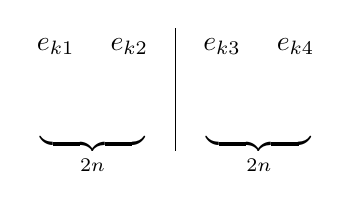
\begin{tikzpicture}[x=.76cm,y=.76cm]
\node at (0,0) {\(e_{k1}\)};
\node at (1.23,0) {\(e_{k2}\)};
\node at (2.78,0) {\(e_{k3}\)};
\node at (4.01,0) {\(e_{k4}\)};
\draw (2,.3)--(2,-1.75);
\node at (.615,-1.8) {\(\underbrace{\hspace{1.33cm}}_{2n}\)};
\node at (3.395,-1.8) {\(\underbrace{\hspace{1.33cm}}_{2n}\)};
\end{tikzpicture}}\endgroup\par}
\end{GelfandAdjacentEvidence}
\begin{GelfandAdjacentEvidence}{GELFAND-P000744}{5}


At infinity everything becomes trivial.

“An instanton lives only a short while, and in imaginary time at that ---\\
--- a humanoid formation”

Choose from among \(e_{ij}\) a basis of \(H\),\qquad \(B\subset(e_{ij})\)

\(\Leftrightarrow\) \((2n+r)\)-diagonal minor in \(\widetilde Q\)

(one such minor)

Using it, expand the system of generating sections of \(L\).
\[
(22)\qquad \sum X_b\,Q\bigl(b,\underset{h_{k2}}{h_{k1}}\bigr)=0,\qquad
k=1,\ldots,n,\qquad b\in B.
\]
\Unclear{GELFAND-P000744}{equation22}{The manuscript places \(h_{k2}\) below \(h_{k1}\), beneath the parentheses.}
\end{GelfandAdjacentEvidence}


this is a system of \(2n\) eqs. for \(2n+r\) unknowns \(X_b\).

Fund. system of solutions \(X^{(i)}\), \(i=1,\ldots,r\).

Orthonormalize it to obtain \([Y^{(i)}]\) and now write down the answer:


\Needspace{7\baselineskip}
\begin{GelfandAdjacentEvidence}{GELFAND-P000745}{1}
\SourcePage{GELFAND-P000745}{unlabelled}

\SourceFigure{GELFAND-P000745}{formula-bracket}{%
\par\begingroup\color{black}\GelfandFitDiagram{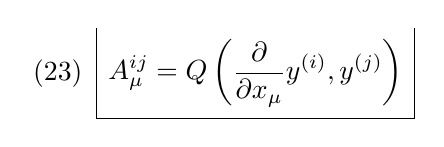
\begin{tikzpicture}
\node[inner sep=4pt] (a) {\(\displaystyle A_\mu^{ij}=Q\left(\frac{\partial}{\partial x_\mu}y^{(i)},y^{(j)}\right)\)};
\node[anchor=east,inner sep=2pt] at ([xshift=-3pt]a.west) {\((23)\)};
\draw (a.north west)--(a.south west)--(a.south east)--(a.north east);
\end{tikzpicture}}\endgroup\par}
\end{GelfandAdjacentEvidence}
\begin{GelfandAdjacentEvidence}{GELFAND-P000745}{2}

\Unclear{GELFAND-P000745}{formula-y-case}{Both letters in (23) have descenders and read as lowercase \(y\).}
\end{GelfandAdjacentEvidence}
\begin{GelfandAdjacentEvidence}{GELFAND-P000745}{3}


\(X^{(i)}\) --- rational functions with values in \(H\);

roots of rational functions arise in orthonormalization.

\uwave{Geometric theorem}.

The diagrams \(I\subset H\otimes\mathbb C^4\) with certain cond. \ldots

classify bundles over \(\mathbb{C}P^3\) with conditions.

1) \(H^i(L(-2))=0\) and likewise for \(L^*\);
\Unclear{GELFAND-P000745}{cohomology-index}{The dot of the superscript \(i\) is visible along the thin horizontal streak in the scan.}
\end{GelfandAdjacentEvidence}


2) \(H^2(L(-1))=0\);

3) \(H^0(L(-1))=0\).


\Needspace{7\baselineskip}
\begin{GelfandAdjacentEvidence}{GELFAND-P000746}{1}
\SourcePage{GELFAND-P000746}{15}

\underline{28/\(\overline{\underline{\mathrm{XI}}}\)-77.}\qquad
\underline{Gelfand Sem.}

\fcolorbox{red}{white}{\underline{\underline{L. D. Faddeev.}}}\qquad
\underline{Solitons as particles.}

I. \(u(x,t)\) --- a field, \(x\in\mathbb R^d\), \(d=1,2,3\).

\[
\Box=\frac{\partial^2}{\partial t^2}-\frac{\partial^2}{\partial x^2}
\]
\begin{equation*}
\Box u+m^2u+\varepsilon V'(u)=0
\tag{1}
\end{equation*}
\begin{equation*}
\mathcal L=\int\left[\tfrac12\,\partial u\cdot\partial u
-\tfrac12 m^2u^2-\varepsilon V(u)\right]dx
\tag{2}
\end{equation*}
\[
\partial_0u(x,t)\underset{\mathrm{def}}{=}\pi(x,t)
\]
\begin{equation*}
\{u(x,t),\pi(y,t)\}=\delta(x-y)
\tag{3}
\end{equation*}
\begin{equation*}
H=\int\left[\tfrac12\pi^2+\tfrac12(\nabla u)^2
+\tfrac12m^2u^2+\varepsilon V(u)\right]dx
\tag{4}
\end{equation*}

\uwave{Free field}: \(\varepsilon=0\)

In quantum theory \(u,\pi\) --- operators.

Fourier transf. for \(\varepsilon=0\):
\begin{equation*}
H=\int\sqrt{k^2+m^2}\,a^*(k)a(k)\,dk
\tag{5}
\end{equation*}
\begin{equation*}
\{a^*(k),a(k')\}=i\delta(k-k')
\tag{6}
\end{equation*}

\uwave{Quantization}: let \(a,a^*\) --- operators, the operator
\begin{equation*}
\hat\rho(k)=\hat a^*(k')\hat a(k)
\tag{7}
\end{equation*}
\Unclear{GELFAND-P000746}{eq7-argument}{A prime is visible on \(k'\) in the first factor. The \(k\) in the second factor has no prime.}
\end{GelfandAdjacentEvidence}
\begin{GelfandAdjacentEvidence}{GELFAND-P000746}{2}


has eigenvalues:
\begin{equation*}
\rho'(k)=\sum\left[\delta(k-k_1)+\dots+\delta(k-k_n)\right]
\tag{8}
\end{equation*}
\Unclear{GELFAND-P000746}{eq8-summation}{After the equals sign comes \(\sum\) without limits, then a square bracket.}
\end{GelfandAdjacentEvidence}


\uwave{The spectrum of the Hamiltonian is interpreted in terms of particles}.
\begin{equation*}
E(k_1,\dots,k_n)=\omega(k_1)+\dots+\omega(k_n),\qquad
\omega=\sqrt{k^2+m^2}
\tag{9}
\end{equation*}

(see: analogy with the oscillator)


\Needspace{7\baselineskip}
\begin{GelfandAdjacentEvidence}{GELFAND-P000747}{1}
\SourcePage{GELFAND-P000747}{unlabelled}

\uwave{In classical terms}: if a finite-energy soln. of eq. (1) asymptotically approaches at \(\infty\) a soln. of the free eq., then this picture is natural.
\Unclear{GELFAND-P000747}{top-cancelled-word}{The crossed-out word tentatively reads “Тогда” (then).}
\end{GelfandAdjacentEvidence}
\begin{GelfandAdjacentEvidence}{GELFAND-P000747}{2}

Then \(H(u)=H(u_0)\), since \(H\) --- an integral.

Solitons are a counterexample to this hypothesis.

\uwave{Solitons}: “everything that fails to satisfy the condition \(u\to u_0\) as \(|t|\to\infty\)”

“Definition”: \uwave{a soliton is something that}
\Unclear{GELFAND-P000747}{definition-cancelled-start}{The crossed-out fragment tentatively reads “не уд” (beginning of “does not satisfy”).}
\end{GelfandAdjacentEvidence}
\begin{GelfandAdjacentEvidence}{GELFAND-P000747}{3}

\uwave{does not spread out at infinity while having finite energy}.

\uwave{Example}: a solution of the stationary eq..

\(u_s(x)\) --- one solution \(\Rightarrow\) a Lorentz transf. gives
\Unclear{GELFAND-P000747}{eq10-deleted-factor}{A heavily crossed-out entry precedes the left parenthesis. \(u_s\) is written above it.}
\end{GelfandAdjacentEvidence}
\begin{GelfandAdjacentEvidence}{GELFAND-P000747}{4}

\begin{equation*}
u_s\left(\frac{x-x_0-vt}{\sqrt{1-v^2}}\right)=u_s(x,t\mid x_0,v)
\tag{10}
\end{equation*}
\Unclear{GELFAND-P000747}{eq10-right-correction}{There is a small crossed-out mark at the right end of the fraction bar. The parenthesis is retraced and extended downward.}
\end{GelfandAdjacentEvidence}
\begin{GelfandAdjacentEvidence}{GELFAND-P000747}{5}


already a soliton, depending on 2 parameters.

At large times: if \(v_1\ne v_2\) then
\begin{equation*}
u(x,t\mid x_{01},v_1)+u(x,t\mid x_{02},v_2)
\tag{11}
\end{equation*}
is asymptotically a solution.

Then the asymptotics: as \(|t|\to\infty\)
\begin{equation*}
u\to u_0+\sum u(x,t\mid v_i,x_{0i})
\tag{12}
\end{equation*}
\Unclear{GELFAND-P000747}{eq12-argument-order}{After the vertical bar the manuscript reads \(v_i,x_{0i}\).}
\end{GelfandAdjacentEvidence}


(a hypothesis in general; a theorem in models)

As \(t\to+\infty\) and as \(t\to-\infty\) they differ.

Energy
\begin{equation*}
H(u)=H(u_0)+\sum_{i=1}^{n}H_s(v_i)
\tag{13}
\end{equation*}
It is clear from the relativistic formula that
\begin{equation*}
H_s(v)=\frac{M}{\sqrt{1-v^2}}=\sqrt{p^2+M^2}
\qquad\text{(“soliton energy”)}
\tag{14}
\end{equation*}

\(M\) --- the energy of a static soliton (“mass” by definition).

(14) --- the definition of \(p\).

This gives 2 parts of phase space. Energy:
\begin{equation*}
\int\omega(k)\rho(k)\,dk+\sum_i^n\sqrt{p_i^2+M^2}
\tag{15}
\end{equation*}

Solitons contributed already in the classical theory. In quantum mechanics there enters \(\dfrac{M}{\hbar c}\);
solitons persist as \(\hbar\to+0\).


\Needspace{7\baselineskip}
\begin{GelfandAdjacentEvidence}{GELFAND-P000748}{1}
\SourcePage{GELFAND-P000748}{16}

In quantum mechanics the spectrum will be
\begin{equation*}
\sum_{i=1}^{N}\sqrt{k_i^2+m^2}+\sum_i^n\sqrt{p_i^2+M^2}
\tag{16}
\end{equation*}
From one field, 2 kinds of particles (semiclassically)

\uwave{Periodic solution.}
\begin{equation*}
u_p(x,t\mid x_0,\bar v,\beta,\alpha)
\tag{17}
\end{equation*}
\Unclear{GELFAND-P000748}{eq17-beta}{The retraced sign tentatively reads \(\beta\).}
\end{GelfandAdjacentEvidence}
\begin{GelfandAdjacentEvidence}{GELFAND-P000748}{2}

\(\beta\) is related to \(T\) (period), \(\alpha\) (initial phase) are parameters

In this case
\begin{equation*}
\sum_{i=1}^{N}\sqrt{k^2+m^2}+\sum_i^n\sqrt{p_i^2+M^2}
+\sum_k^\tau\sqrt{p_k^2+M(\alpha_k)}
\tag{18}
\end{equation*}
\Unclear{GELFAND-P000748}{eq18-first-radicand}{The first radicand reads \(k^2\), with no visible subscript.}
\end{GelfandAdjacentEvidence}
\begin{GelfandAdjacentEvidence}{GELFAND-P000748}{3}

\Unclear{GELFAND-P000748}{eq18-upper-index}{The last upper summation limit tentatively reads \(\tau\). Another possible reading is \(r\).}
\end{GelfandAdjacentEvidence}
\begin{GelfandAdjacentEvidence}{GELFAND-P000748}{4}

\Unclear{GELFAND-P000748}{eq18-last-radicand}{The last radicand has \(M(\alpha_k)\), with no visible exponent \(2\).}
\end{GelfandAdjacentEvidence}
\begin{GelfandAdjacentEvidence}{GELFAND-P000748}{5}


\uwave{The main model problem:}
\begin{equation*}
v(u)=1-\cos u-\frac{u^2}{2}
\tag{19}
\end{equation*}
\Unclear{GELFAND-P000748}{eq19-potential-glyph}{The initial sign before \((u)\) is rendered as \(v\). It may be \(\upsilon\).}
\end{GelfandAdjacentEvidence}
\begin{GelfandAdjacentEvidence}{GELFAND-P000748}{6}

The eq. takes the form:
\begin{equation*}
\Box u+m^2\sin u=0
\tag{20}
\end{equation*}
(the \((\sin\varphi)_2\))

One more parameter: in the Poisson bracket put
\begin{equation*}
\{\partial_0u,u\}=\gamma\delta(\ldots)
\tag{21}
\end{equation*}
Then it turns out that
\begin{equation*}
M=\frac{8m}{\gamma}\qquad\text{(“heavy particle”)}
\tag{22}
\end{equation*}
\begin{equation*}
M_2(\alpha)=\frac{16m}{\gamma}\sin\alpha,\qquad 0<\alpha\leq\frac{\pi}{2}.
\tag{23}
\end{equation*}
These \Unclear{GELFAND-P000748}{cancelled-word}{The crossed-out word tentatively reads “двумя” (two).}
\end{GelfandAdjacentEvidence}

solutions determine everything.

Here one must take
\begin{equation*}
\alpha=\frac{\gamma}{16}n,\quad n=1,2,\ldots
\tag{24}
\end{equation*}
(Takhtajan, \underline{Faddeev}, \(\approx1974\) )

A detailed review (in English) should appear shortly.


\Needspace{7\baselineskip}
\begin{GelfandAdjacentEvidence}{GELFAND-P000749}{1}
\SourcePage{GELFAND-P000749}{unlabelled}

\underline{II.} \uwave{Consistent quantization and the \(S\)-matrix}.

It has not yet been possible to find the actual eigenfunctions.
\Unclear{GELFAND-P000749}{eigenfunction-abbreviation}{The abbreviation in the first sentence reads “соб.” (eigenfunctions).}
\end{GelfandAdjacentEvidence}
\begin{GelfandAdjacentEvidence}{GELFAND-P000749}{2}

 But the \(S\)-matrix has been computed! (by an indirect route: the path integral)

Definitions: write
\begin{equation*}
H=\int\left[\frac{\pi^2}{2}+\frac{(\nabla u)^2}{2}+\frac{m^2}{2}u^2+V(u)\right]
\tag{25}
\end{equation*}
and take \(\pi\) and \(u\) to be operators with the relation
\begin{equation*}
[\hat\pi(x),\hat u(y)]=i\delta(x-y)
\tag{26}
\end{equation*}
There is no contradiction, but one must begin with renormalizations.

\uwave{Glimm, Jaffe:}

\uwave{Frohlich}
\Unclear{GELFAND-P000749}{latin-surname}{The middle letters of the surname are unclear. The tentative reading is “Frohlich”.}
\end{GelfandAdjacentEvidence}
\begin{GelfandAdjacentEvidence}{GELFAND-P000749}{3}

\[
\left[\begin{gathered}
\frac{m^2}{\gamma}(1-\cos\gamma u)\quad\text{for small }\gamma\quad\text{constructed}\\
\text{the Hamiltonian rigorously}\quad(\text{for }x\in\mathbb R^1).
\end{gathered}\right.
\]
\Unclear{GELFAND-P000749}{small-coupling}{The denominator and the factor before \(u\) read \(\gamma\), with no visible exponent \(2\).}
\end{GelfandAdjacentEvidence}
\begin{GelfandAdjacentEvidence}{GELFAND-P000749}{4}


\underline{Lemma 1} (from ordinary quantum mechanics). \uwave{Consider the eq.}
\begin{equation*}
i\frac{\partial\Psi}{\partial t}=H\Psi
\tag{27}
\end{equation*}
\begin{equation*}
H=-\frac{\Delta}{2m}+v(x),\quad v\text{ decays rapidly}
\tag{28}
\end{equation*}
\Unclear{GELFAND-P000749}{eq28-potential}{The rounded sign before \((x)\) and later in the line is rendered as \(v\). It may be \(\upsilon\).}
\end{GelfandAdjacentEvidence}

\uwave{Then the limit exists}
\begin{equation*}
S=\lim_{\substack{t''\to\infty\\t'\to-\infty}}
e^{iH_0t''}e^{-iH(t''-t')}e^{-iH_0t'}
\tag{29}
\end{equation*}
(\(S\)-matrix) \uwave{and} \(S\) --- \uwave{a unitary operator}.

It is better to work in the momentum representation: the kernel is denoted by \(S(p'',p')\). It suffices to know the kernel of the evolution op.
\(e^{-iH(t''-t')}=K\)
\[
K(x'',t''\mid x',t')
\]
One must take
\begin{equation*}
\begin{cases}
x''=\dfrac{p''}{m}t''\\
x'=\dfrac{p'}{m}t'
\end{cases}
\tag{30}
\end{equation*}
(by the classical formulas with the free \(H_0\)). Then
\begin{equation*}
S(p'',p')=\lim_{\substack{t''\to+\infty\\t'\to-\infty}}
\frac{K\left(\frac{p''}{m}t'',t''\mid\frac{p'}{m}t',t'\right)}
{K_0\left(\frac{p''}{m}t'',t''\mid0,0\right)
K_0\left(0,0\mid\frac{p'}{m}t',t'\right)}
\tag{31}
\end{equation*}
(analogous to (29))


\Needspace{7\baselineskip}
\begin{GelfandAdjacentEvidence}{GELFAND-P000750}{1}
\SourcePage{GELFAND-P000750}{17}

The right-hand side of (31) is computed by a path integral over trajectories with classical asymptotics.

\uwave{Comment on} (31): apply it to \(\Psi\), considering a wave packet
\begin{equation*}
\Psi(x,t)=\left[\frac1{2\pi}\int\Psi(p)e^{ipx}e^{-i\frac{p^2}{2m}t}\,dp\right]
\underset{\substack{\uparrow\\\text{stationary-phase}\\\text{method}}}{\cong}
\widetilde\Psi\left(\frac{mx}{t}\right)e^{i\frac{x^2}{2mt}}
\tag{32}
\end{equation*}
\Unclear{GELFAND-P000750}{eq32-integrand-psi}{A short mark appears above the \(\Psi\) under the integral. A tilde is uncertain.}
\end{GelfandAdjacentEvidence}
\begin{GelfandAdjacentEvidence}{GELFAND-P000750}{2}

\Unclear{GELFAND-P000750}{eq32-exponent-overwrite}{The last denominator symbol in the exponential is heavily retraced and tentatively reads \(t\).}
\end{GelfandAdjacentEvidence}
\begin{GelfandAdjacentEvidence}{GELFAND-P000750}{3}

\[
\Psi(t)=e^{-iH_0t'}\Psi
\]
\Unclear{GELFAND-P000750}{unnumbered-time-argument}{The left side reads \(\Psi(t)\), while the exponential on the right has \(t'\).}
\end{GelfandAdjacentEvidence}
\begin{GelfandAdjacentEvidence}{GELFAND-P000750}{4}

We obtain
\begin{equation*}
K(.\ .\mid\tfrac{p}{m}t,t)\,\widetilde\Psi(p)\sqrt{\frac mt}\,dp
\tag{33}
\end{equation*}
with factors (in each part we pass to its own coordinate system).
\SourceFigure{GELFAND-P000750}{triangle}{%
\par\begingroup\color{black}\GelfandFitDiagram{
\begin{tikzpicture}
\fill (0,0)--(.03,.30)--(.34,.19)--cycle;
\end{tikzpicture}}\endgroup\par}
\end{GelfandAdjacentEvidence}
\begin{GelfandAdjacentEvidence}{GELFAND-P000750}{5}


\underline{Path integral.} First for quantum mechanics
\begin{equation*}
K(x'',t''\mid x',t')=\frac1N\int
e^{i\int_{t'}^{t''}\left[\frac{m\dot x^2}{2}-v(x)\right]dt}
\prod_{t'\leq t\leq t''}dx(t),
\tag{34}
\end{equation*}
\Unclear{GELFAND-P000750}{eq34-potential}{The first sign in \(v(x)\) is rounded. It may be \(\upsilon\).}
\end{GelfandAdjacentEvidence}
\begin{GelfandAdjacentEvidence}{GELFAND-P000750}{6}

over trajectories such that
\begin{equation*}
x(t')=x',\quad x(t'')=x''
\tag{35}
\end{equation*}
\(N\) --- a normalization factor (depending on time).

Now one must take \(x(t')=\dfrac{pt'}m\), \(x(t'')=\dfrac{pt''}m\).

In field theory one must write
\begin{equation*}
K(u''(x),t''\mid u'(x),t')=\frac1N\int
\exp\left\{i\int\mathcal L(x)\,dx\right\}
\prod_{\substack{t'\leq t\leq t''\\-\infty<x<\infty}}
du\,\text{[crossed out]}(x,t)
\tag{36}
\end{equation*}
\Incomplete{GELFAND-P000750}{eq36-cancelled-argument}{There is a crossed-out fragment after \(du\) and before \((x,t)\). Its reading is undetermined.}
\end{GelfandAdjacentEvidence}
\begin{GelfandAdjacentEvidence}{GELFAND-P000750}{7}

over \(u\), such that
\begin{equation*}
\begin{cases}
u(x,t'')=u''(x)\\
u(x,t')=u'(x)
\end{cases}
\tag{37}
\end{equation*}
For the initial and final configurations one must take sums of solitons. This gives transition probabilities.

There is as yet no good quantum version of the inverse problem.
\Unclear{GELFAND-P000750}{good-word-crossing}{A thin diagonal stroke crosses the end of “Хорошего” (good) and continues downward to the right.}
\end{GelfandAdjacentEvidence}
\begin{GelfandAdjacentEvidence}{GELFAND-P000750}{8}


For the \(S\)-matrix of sine-Gordon, an exact formula has been guessed
(\uwave{Zamolodchikov} from ITEP; see Comm. on Math. Physics)

\Incomplete{GELFAND-P000750}{hypothesis-prefixed-mark}{Crossed-out strokes and part of a rectangular box precede “Гипотеза” (hypothesis). Their reading is undetermined.}
\end{GelfandAdjacentEvidence}

Hypothesis: all classically solvable problems are also solvable in the quantum version


\Needspace{7\baselineskip}
\begin{GelfandAdjacentEvidence}{GELFAND-P000751}{1}
\SourcePage{GELFAND-P000751}{unlabelled}

\begin{equation*}
\langle u''(x)\mid e^{-iH(t''-t')}\mid u'(x)\rangle
\tag{38}
\end{equation*}
--- a matrix element given by the path integral. Now one must divide and let \(t\) tend to \(\pm\infty\).

Corrections to the
\Incomplete{GELFAND-P000751}{top-cancel}{A short fragment between “к” (to) and “классической” (classical) is crossed out and undeciphered.}
\end{GelfandAdjacentEvidence}
\begin{GelfandAdjacentEvidence}{GELFAND-P000751}{2}

classical mass arise already for a single soliton.

\uwave{Problems arising in the computation of the integral.}

The stationary-phase method.
\begin{equation*}
u(x,t)=U_{cl}(x,t)+\sqrt h\,\varphi(x,t)+\ldots
\tag{39}
\end{equation*}
\Incomplete{GELFAND-P000751}{cancel-before-operator}{A phrase preceding “Возникает оператор” (the operator arises) is heavily crossed out. Its reading is undetermined.}
\end{GelfandAdjacentEvidence}
\begin{GelfandAdjacentEvidence}{GELFAND-P000751}{3}

The operator arises
\begin{equation*}
A\varphi=\Box\varphi+m^2\varphi+V''(u_\varphi)\varphi
\tag{40}
\end{equation*}
\Unclear{GELFAND-P000751}{operator-mass-term}{The heavily retraced signs after \(m^2\) tentatively read \(\varphi+\).}
\end{GelfandAdjacentEvidence}
\begin{GelfandAdjacentEvidence}{GELFAND-P000751}{4}

\Unclear{GELFAND-P000751}{operator-u-index}{The subscript on \(u\) tentatively reads \(\varphi\).}
\end{GelfandAdjacentEvidence}
\begin{GelfandAdjacentEvidence}{GELFAND-P000751}{5}

Corrections are computed through \(\det A\).

It is expressed through the \(S\)-matrix for an auxiliary linear equation. Loops arise next.
One needs the inverse operator \(R=A^{-1}\) and the kernel \underline{\(R(x,y)\)}, namely
\begin{equation*}
\int R^3(x,x)\,d^2x
\tag{41}
\end{equation*}
\uwave{Hopes}: it is possible that such functionals can be computed explicitly.
\Unclear{GELFAND-P000751}{cancel-quadratures}{The crossed-out phrase tentatively reads “в квадратурах” (by quadratures).}
\end{GelfandAdjacentEvidence}
\begin{GelfandAdjacentEvidence}{GELFAND-P000751}{6}


Let \(u_1\) --- a one-soliton solution (stationary),
\begin{equation*}
V''(u_1(x))=q(x).
\tag{42}
\end{equation*}
Computing
\begin{equation*}
\det\left(\frac{d^2}{dt^2}-\frac{d^2}{dx^2}+q(x)\right)
\tag{43}
\end{equation*}
reduces to the spectral density of the stationary op. (the variables separate). One obtains \(q(x)=\frac1{\operatorname{ch}^2x}\)
and all eigenfunctions are found explicitly (the simplest Bargmann potential).

\(\det A\) is expr. through the eigenfunction with zero eigenvalue.

Corrections to the mass of the
\Incomplete{GELFAND-P000751}{cancel-before-soliton}{A short word before “солитона” (soliton) is heavily crossed out and undeciphered.}
\end{GelfandAdjacentEvidence}
\begin{GelfandAdjacentEvidence}{GELFAND-P000751}{7}

soliton:
\begin{equation*}
M=\frac{8m}{\gamma}-\frac m\pi+O(\gamma)
\tag{44}
\end{equation*}
\underline{Conjecture}: for sine-Gordon
\begin{equation*}
M=\frac{8m}{\gamma}-\frac m\pi,
\tag{45}
\end{equation*}
i.e. there are no higher corrections. (justif. by Zamolodchikov)
\Unclear{GELFAND-P000751}{justified-abbreviation}{The abbreviation before the surname tentatively reads “оправд.” (justified). Its first letter may be “с”.}
\end{GelfandAdjacentEvidence}


For \(\gamma\leq8\pi\) everything is fine, and beyond this the soliton disappears.


\Needspace{7\baselineskip}
\begin{GelfandAdjacentEvidence}{GELFAND-P000752}{1}
\SourcePage{GELFAND-P000752}{18}

\uwave{Formulas for the \(S\)-matrix of sine-Gordon.}

One must compute the abbreviated action for the 2-soliton solution.
\begin{equation*}
S_{sa}(p_1'',p_2'';p_1',p_2')
=\delta(p_1''-p_1')\delta(p_2''-p_2')e^{i\Theta(p_1,p_2)}
\tag{46}
\end{equation*}
\Unclear{GELFAND-P000752}{equation-46-separator}{The separator between the arguments is heavily retraced. It is tentatively rendered as a semicolon.}
\end{GelfandAdjacentEvidence}
\begin{GelfandAdjacentEvidence}{GELFAND-P000752}{2}

(There is a soliton and an antisoliton)

The action (classical)
\begin{equation*}
\Theta=\frac8\gamma\int_0^\pi d\alpha
\left[\ln\frac{e^{i(\beta-\alpha)}+1}{e^{i\beta}+e^{-i\alpha}}\right]
\tag{47}
\end{equation*}
[Crossed out: For \(\gamma=\frac{8\pi}{N}\), \(N\) --- an integer]
\Incomplete{GELFAND-P000752}{cancel-after-47}{The end of the crossed-out line following “целое” (integer) is undeciphered.}
\end{GelfandAdjacentEvidence}
\begin{GelfandAdjacentEvidence}{GELFAND-P000752}{3}

(the integral cannot be evaluated).

One must take \(\gamma=\frac{8\pi}{N}\), \(N\) --- an integer
\begin{equation*}
\Theta\longrightarrow\sum\ln(\ldots)
\tag{48}
\end{equation*}
Zamolodchikov took this to hold for \(\gamma=\frac{8\pi}{N}\) and interpolated.

As a result sine-Gordon turned out to resemble a quantum-mechanical system [Crossed out: and] with
\begin{equation*}
H=-\frac{d^2}{dx^2}+\frac{a}{\operatorname{ch}^2\alpha x}
\tag{49}
\end{equation*}
\Unclear{GELFAND-P000752}{potential-numerator}{The numerator tentatively reads \(a\), possibly \(q\).}
\end{GelfandAdjacentEvidence}
\begin{GelfandAdjacentEvidence}{GELFAND-P000752}{4}

[Crossed out: Eigenvalue \(\alpha(\ell+\tfrac12)^2\)]
\Unclear{GELFAND-P000752}{cancel-eigenvalue-formula}{The crossed-out formula tentatively reads \(\alpha(\ell+\tfrac12)^2\).}
\end{GelfandAdjacentEvidence}
\begin{GelfandAdjacentEvidence}{GELFAND-P000752}{5}

\Incomplete{GELFAND-P000752}{cancel-eigenvalue-end}{The end of the crossed-out line is undeciphered. A fragment tentatively reads “с пр…”.}
\end{GelfandAdjacentEvidence}
\begin{GelfandAdjacentEvidence}{GELFAND-P000752}{6}


\underline{A remarkable dynamical system}

is associated with a field (chiral)
\begin{equation*}
n(x):R^2\longrightarrow S^n\subset R^{n+1}
\tag{50}
\end{equation*}
\begin{equation*}
\mathcal L=\frac12\int\partial n\cdot\partial n\,dx
\tag{51}
\end{equation*}
it is nontrivial because of its values (there is nonlinearity).

\(L\)-\(A\) pair has been written down ([Crossed out: Fol; written above: Pol]meyer (?); Zakharov and Mikhailov)
\Unclear{GELFAND-P000752}{name-correction}{The beginning of the surname is corrected from tentative “Фоль” (Fol) to “Поль” (Pol).}
\end{GelfandAdjacentEvidence}
\begin{GelfandAdjacentEvidence}{GELFAND-P000752}{7}


[Crossed out: Na]
\Incomplete{GELFAND-P000752}{cancel-before-quantization}{The remainder of the crossed-out phrase before “Квантование” (quantization) is undeciphered.}
\end{GelfandAdjacentEvidence}

Quantization is weakly connected with the classical theory.

Massive particles appear as solitons.

There will be a talk on this at the seminar named after I. G. Petrovsky.


\Needspace{7\baselineskip}
\begin{GelfandAdjacentEvidence}{GELFAND-P000753}{1}
\SourcePage{GELFAND-P000753}{unlabelled}

\underline{13/II-78.}\qquad \uwave{Gelfand Seminar.}

\underline{I. M. G.} there are 2 primary concepts in category theory:
1) Topos\quad 2) Derived category.

\SourceFigure{GELFAND-P000753}{speaker-box}{\begingroup\color{black}\GelfandFitDiagram{\begin{tikzpicture}
\node[draw=red,inner sep=3pt,text=black]{\underline{S. Gelfand}};
\end{tikzpicture}}\endgroup}
\end{GelfandAdjacentEvidence}
\begin{GelfandAdjacentEvidence}{GELFAND-P000753}{2}


\underline{Problem}: describe all algebraic bundles over
\Incomplete{GELFAND-P000753}{cancel-before-projective}{A short sign before the projective-space notation is heavily crossed out.}
\end{GelfandAdjacentEvidence}
\begin{GelfandAdjacentEvidence}{GELFAND-P000753}{3}

\(\mathbb P^n\).
(\(n\)-dimensional projective space; for example, over \(\mathbb C\)).

\(\Xi\) --- affine space.
\[
\xi\sim\alpha\xi,\quad \alpha\in\mathbb C^*,\quad (\xi\ne0);
\qquad \text{Then}\ \Xi/{\sim}=\mathbb P^n.
\]
\Unclear{GELFAND-P000753}{scalar-choice}{The multiplier and the following sign are tentatively read as \(\alpha\).}
\end{GelfandAdjacentEvidence}
\begin{GelfandAdjacentEvidence}{GELFAND-P000753}{4}


\(\Lambda\) --- the Grassmann algebra in \((n+1)\)-th variable
(\Incomplete{GELFAND-P000753}{cancel-before-algebra}{An abbreviation at the beginning of the parentheses is heavily crossed out; its reading is unresolved.}
\end{GelfandAdjacentEvidence}
\begin{GelfandAdjacentEvidence}{GELFAND-P000753}{5}

algebra over \(\Xi\)).
\[
\Lambda=\{\xi_0,\ldots,\xi_n\mid
\xi_i\xi_j+\xi_j\xi_i=0\}.
\]
\[
\dim\Lambda=2^{n+1}.
\]
Introduce a grading on \(\Lambda\):
\begin{equation*}
\Lambda=\Lambda_0\oplus\Lambda_{-1}\oplus\cdots\oplus\Lambda_{-(n+1)},
\qquad [\text{Crossed out: }\Lambda_0\text{ --- the field of constants}]
\tag{1}
\end{equation*}
where
\[
\Lambda_{-k}\ [\text{Crossed out: }\Lambda_k?]
=\{\xi_{i_1}\cdots\xi_{i_k}\},\qquad
\Lambda_0\text{ --- the field of constants}.
\]
\Unclear{GELFAND-P000753}{cancel-grading-symbol}{The cancelled expression before the equality sign tentatively reads \(\Lambda_k\).}
\end{GelfandAdjacentEvidence}
\begin{GelfandAdjacentEvidence}{GELFAND-P000753}{6}


\uwave{Objects}: a graded finite-dimensional representation of
\(\Lambda\) or a graded \(\Lambda\)-module:
\begin{equation*}
V=\bigoplus V_j,\qquad \dim V<\infty.
\tag{2}
\end{equation*}
\begin{equation*}
\Lambda_{-k}V_j\subset V_{j-k}.
\tag{3}
\end{equation*}

Let \(\xi_0,\ldots,\xi_n\) --- be a basis in \(\Xi\), \(\xi\in\Xi\).
\begin{equation*}
\xi=c_0\xi_0+\cdots+c_n\xi_n.
\tag{4}
\end{equation*}
\((-k)\) --- for historical reasons (from Serre's paper).

Then \(\xi:V_j\longrightarrow V_{j-1}\).
Hence, since \(\deg\xi=-1\), we have
\SourceFigure{GELFAND-P000753}{complex-diagram}{\begingroup\color{black}\GelfandFitDiagram{\begin{tikzcd}[ampersand replacement=\&,column sep=large]
\cdots\arrow[r]\&V_1\arrow[r,"\xi"]\&V_0\arrow[r,"\xi"]\&
V_{-1}\arrow[r]\&\cdots
\end{tikzcd}}\endgroup}
\end{GelfandAdjacentEvidence}
\begin{GelfandAdjacentEvidence}{GELFAND-P000753}{7}


\(\xi^2=0\ \Rightarrow\) we have obtained a complex.

Thus, from an element \(\xi\ne0\) and a module \(V\) one constructs the complex
\begin{equation*}
L_\xi(V)=
\{\cdots\longrightarrow V_1\xrightarrow{\xi}V_0
\xrightarrow{\xi}V_{-1}\longrightarrow\cdots\}.
\tag{5}
\end{equation*}

\uwave{Definition}. \(V\) is called \dashuline{proper}, if
\begin{equation*}
\forall\xi\ne0,\qquad H_i(L_\xi(V))=0\quad\text{for }i\ne0.
\tag{6}
\end{equation*}
Here:
\begin{equation*}
H_i\ [\text{Crossed out: ?}]\ (L_\xi(V))
=\ker(V_i\longrightarrow V_{i-1})/
\operatorname{Im}(V_{i+1}\longrightarrow V_i)
\tag{7}
\end{equation*}
\Incomplete{GELFAND-P000753}{cancel-homology-symbol}{A sign between the index and the parenthesis in (7) is heavily crossed out.}
\end{GelfandAdjacentEvidence}
\begin{GelfandAdjacentEvidence}{GELFAND-P000753}{8}

\Unclear{GELFAND-P000753}{homology-equation-number}{The equation number is heavily retraced; it tentatively reads (7).}
\end{GelfandAdjacentEvidence}
\begin{GelfandAdjacentEvidence}{GELFAND-P000753}{9}


--- [Crossed out: quotient spaces?]
\Unclear{GELFAND-P000753}{cancel-homology-word}{The crossed-out word tentatively reads “факторпространства” (quotient spaces); its beginning is obscured by dense strokes.}
\end{GelfandAdjacentEvidence}

\uwave{homology of the complex}.


\Needspace{7\baselineskip}
\begin{GelfandAdjacentEvidence}{GELFAND-P000754}{1}
\SourcePage{GELFAND-P000754}{43}

In this case
\[
\dim H_0^{?}(L_\xi(V))=\mathrm{const}
\]
\Unclear{GELFAND-P000754}{top-homology-mark}{A dense mark appears above \(H_0\); its internal strokes cannot be distinguished. A question mark represents it in the typeset formula.}
\end{GelfandAdjacentEvidence}
\begin{GelfandAdjacentEvidence}{GELFAND-P000754}{2}

(does not depend on \(\xi\))

by Euler's formula

(left side — the Euler characteristic \(\xi\)?
\Unclear{GELFAND-P000754}{euler-overwritten-mark}{The overwritten mark after “характеристика” (characteristic) may be \(\xi\).}
\end{GelfandAdjacentEvidence}
\begin{GelfandAdjacentEvidence}{GELFAND-P000754}{3}

equal to \(\sum(-1)^i\dim V_i\).)

Bundle: \(\xi\longmapsto H_0(L_\xi(V))\).

[Crossed out: If \(\xi\) and]
\Unclear{GELFAND-P000754}{cancelled-line}{The short crossed-out line tentatively reads “Если ξ и” (If ξ and).}
\end{GelfandAdjacentEvidence}


For \(\xi\) and \(\alpha\xi\) it is the same (there is a natural isomorphism).

\uwave{Example}. \(V=\Lambda\) (the regular representation).

\(V_j=\Lambda_j\) (the same grading as before).

\uwave{Answer}:
\(H_i(L_\xi(V))=0,\quad\forall i,\quad\forall\xi\ne0\).

We obtain the zero bundle.

Direct sums give the same result.

\(V_j=\Lambda_{j+\ell}\quad(\ell\text{ --- fixed})\)

\(\Rightarrow\) we again obtain a trivial bundle.

Hence free modules lead to trivial bundles.

\uuline{Theorem 1}
\uwave{Every bundle is obtained by such a construction,
and \(V\) is determined uniquely up to adding a free module.}

(Bernstein, S. Gelfand, I. Gelfand;
independently a similar result by Beilinson, a 3rd-year student)

\dashuline{Refinement of the bundle construction.}

\(V\) --- an arbitrary \(\Lambda\)-module.

\(O(k)\) --- the standard bundles
(their sections are homogeneous rational functions of degree \(k\in\mathbb Z\)), one-dimensional.

Consider
\begin{equation*}
\mathcal L_j=V_{-j}\otimes O(j).
\tag{8}
\end{equation*}
--- a bundle over \(\mathbb P^n\);
each fiber is multiplied by \(V_{-j}\).

\(O(1)\) --- the one that has a section.

Construct
\begin{equation*}
d:\mathcal L_j\longrightarrow\mathcal L_{j+1}.
\tag{9}
\end{equation*}
\(f(\xi)\) --- a section of \(\mathcal L_j\) over an open set

a homogeneous function of degree \(j\) with values in \(V_{-j}\)
\begin{equation*}
d(f(\xi))=\xi(f(\xi)).
\tag{10}
\end{equation*}
(on the right is the action of \(\xi\) on \(V_{-j}\), giving \(V_{-j-1}\)).


\Needspace{7\baselineskip}
\begin{GelfandAdjacentEvidence}{GELFAND-P000755}{1}
\SourcePage{GELFAND-P000756}{44}

Now construct 2 \(\Lambda\)-modules
\begin{equation*}
V=C_N\otimes\Lambda
\tag{18}
\end{equation*}
(on \(C_N\) the action is trivial \(\Xi?\);
\Unclear{GELFAND-P000756}{action-overwritten-symbol}{The sign following “действие” (action) is heavily retraced; the reading \(\Xi\) is tentative.}
\end{GelfandAdjacentEvidence}
\begin{GelfandAdjacentEvidence}{GELFAND-P000756}{2}

on \(\Lambda\) the usual action)
\begin{equation*}
V'=C_{N+1}\otimes\Lambda.
\tag{\(18'\)}
\end{equation*}
We have
\begin{equation*}
\partial:V\longrightarrow V'
\tag{19}
\end{equation*}
\begin{equation*}
\partial(c\otimes\lambda)=\sum_{i=0}^n X_i(c)\otimes\xi_i\lambda
\tag{20}
\end{equation*}
The map \(\partial\) does not depend on the basis.
Set \(W=\operatorname{Ker}\partial\).

This is a \(\Lambda\)-module. Now one must shift back \(N\) times
\[
0\longrightarrow W'\longrightarrow P\longrightarrow W\longrightarrow0
\]
\(W\longmapsto W'\) perform \(N\) times
(with a shift of grading).

This is precisely that representation (that same \(\Lambda\)-module)

\underline{I.M.G.}\quad\uwave{Classification of bundles}
--- not quite the right problem (they do not form an abelian category).
One must allow the fibers to change
\Incomplete{GELFAND-P000756}{cancelled-dimension-word}{A short word between “менять” (change) and “размерность” (dimension) is heavily crossed out.}
\end{GelfandAdjacentEvidence}
\begin{GelfandAdjacentEvidence}{GELFAND-P000756}{3}

dimension --- introduce sheaves.
The work being presented develops Serre's theory.

\uwave{Serre's theorem}
\[
\{\text{Sheaves on }\mathbb CP^n\}\Leftrightarrow
\left\{
\begin{array}{l}
\text{finitely generated }\overset{\text{(graded)}}{\text{modules}}\\
\text{over }\mathbb C[x_0,\ldots,x_n]
\end{array}
\Big/
\begin{array}{l}
\text{up to}\\
\text{a finite}\\
\text{number of homogeneous}\\
\text{components}
\end{array}
\right\}
\]

\(\xi?\)
\Unclear{GELFAND-P000756}{book-left-mark}{The separate overwritten sign to the left of the reference may be \(\xi\); its function is unresolved.}
\end{GelfandAdjacentEvidence}
\begin{GelfandAdjacentEvidence}{GELFAND-P000756}{4}

(an article in the collection “Fiber spaces”; 1953).
\Incomplete{GELFAND-P000756}{book-right-cancellation}{A short fragment after the collection reference is crossed out.}
\end{GelfandAdjacentEvidence}
\begin{GelfandAdjacentEvidence}{GELFAND-P000756}{5}


Construct a sheaf from the module \(M\).

Define its sections over \(E_i=\{x.\ x_i\ne0\}\)

[Crossed out: \(\Gamma(E_i,M)?\)]
\Unclear{GELFAND-P000756}{cancelled-section-formula}{The cancelled formula tentatively reads \(\Gamma(E_i,M)\); diagonal strokes obscure the arguments.}
\end{GelfandAdjacentEvidence}

\[
\Gamma(E_i,\underset{\text{our sheaf}}{L})
=\left\{\frac{m}{x_i^s},\
\begin{array}{l}
\deg m=s\\
m\in M
\end{array}\right\}.
\]

\(O(N)\) arises from \(M=\mathbb C[x_0,\ldots,x_n]\)
with shifted grading
\[
M_i=\{\mathbb C[x_0,\ldots,x_n]\}_{i+N}.
\]


\Needspace{7\baselineskip}
\begin{GelfandAdjacentEvidence}{GELFAND-P000757}{1}
\SourcePage{GELFAND-P000757}{unlabelled}

\uuline{27/II-78.}\qquad \underline{Gelfand Seminar.}

\SourceFigure{GELFAND-P000757}{speaker-box}{\begingroup\color{black}\GelfandFitDiagram{\begin{tikzpicture}
\node[draw=red,inner sep=3pt,text=black]{\uwave{S. I. Gelfand}};
\end{tikzpicture}}\endgroup}
\end{GelfandAdjacentEvidence}
\begin{GelfandAdjacentEvidence}{GELFAND-P000757}{2}


\uwave{Problem}: describe algebraic vector bundles over projective space.

\(\Xi\) --- \((n+1)\)-dimensional space (vector).

\(\mathbb P=\mathbb P(\Xi)\) --- projective \(n\)-dimensional space

[Crossed out]
\Incomplete{GELFAND-P000757}{cancelled-word}{A short word before “Выберем базис” (choose a basis) is crossed out; a complete reading is unresolved.}
\end{GelfandAdjacentEvidence}

Choose a basis of \(\Xi\): \(\xi_0,\ldots,\xi_n\)

and let
\[
\Lambda=\Lambda(\Xi)\quad\text{--- the exterior algebra of }\Xi
\]
\[
\Lambda=\bigoplus_{i=-n-1}^{0}\Lambda_i
\]
\(\Lambda\) has generators \(\xi_0,\ldots,\xi_n\) and relations
\(\xi_i\xi_j+\xi_j\xi_i=0,\quad\xi_i^2=0;\)
\[
\Lambda_{-k}=\{\xi_{i_1}\ldots\xi_{i_k}\}.
\]


\Needspace{7\baselineskip}
\begin{GelfandAdjacentEvidence}{GELFAND-P000758}{1}
\SourcePage{GELFAND-P000758}{unlabelled}

\[
\dim\Lambda_{-k}=\binom{n+1}{k}
\]
\uwave{Remark}: let \(\xi\in\Lambda_{-1}\).
Then \(\xi^2=0\).
(and this is equivalent to all the relations).

\dashuline{Object}: a graded finite-dimensional \(\Lambda\)-module
\[
V=\bigoplus_j V_j,\qquad
\lambda\in\Lambda_i,\ v\in V_j\Rightarrow\lambda v\in V_{i+j}
\]
(\(j\) may be arbitrary integers).

From each \(V\) construct a collection of vector bundles over \(\mathbb P(\Xi)\)
and their maps (a complex of bundles).

\(\forall j\) construct the bundles \(O(j)\)

\uwave{3 definitions of} \(O(j)\)

1) transition functions \((z_k/z_\ell)^j\);

2) sections over an open set \(=\) homogeneous rational functions of degree \(j\);

3) \(j\)-th tensor power of the anti-Hopf bundle.

The corresponding sheaf can be defined as follows:
\[
\Gamma(O(j),U)=
\{\text{rational functions of degree }j\text{ without singularities in }\bar U\}
\]
\(U\subset\mathbb P^n\), \(\bar U\) --- the preimage of \(U\) in \(\Xi\)

\uwave{Problem}: why does a one-dimensional bundle result?

\SourceFigure{GELFAND-P000758}{separator}{\begingroup\color{black}\GelfandFitDiagram{\begin{tikzpicture}
\draw (0,0)--(.62,0);
\fill (.91,0) circle (1pt);
\draw (1.22,0)--(1.96,0);
\end{tikzpicture}}\endgroup}
\end{GelfandAdjacentEvidence}
\begin{GelfandAdjacentEvidence}{GELFAND-P000758}{2}


Set
\[
\mathcal L^j=V_{-j}\otimes O(j)\qquad\text{--- a bundle.}
\]
\Unclear{GELFAND-P000758}{middle-index-correction}{The subscript of \(\mathcal L\) is blotted out; \(j\) is written above. The cancelled subscript tentatively reads \(j\).}
\end{GelfandAdjacentEvidence}
\begin{GelfandAdjacentEvidence}{GELFAND-P000758}{3}


\(V_{-j}\) means the constant bundle with fiber \(V_{-j}\)
\[
\Gamma(\mathcal L^j,U)=
\left\{\begin{gathered}
\text{rational functions with values in }V_{-j},\\
\text{homogeneous degree }j,\ \text{nonsingular in }\bar U
\end{gathered}\right\}.
\]
\Unclear{GELFAND-P000758}{sections-index-correction}{In \(\Gamma(\mathcal L^j,U)\) the subscript is also blotted out; \(j\) is written above. The cancelled subscript tentatively reads \(j\).}
\end{GelfandAdjacentEvidence}
\begin{GelfandAdjacentEvidence}{GELFAND-P000758}{4}


Construct the maps:
\[
d:\mathcal L^j\longrightarrow\mathcal L^{j+1}
\]
\dashuline{On sections}: let
\(f(\xi)\in\Gamma(\mathcal L^j,U)\),
\[
\xi\in\Lambda_{-1}=\Xi
\]
\[
(df)(\xi)=\xi[f(\xi)]
\]
(on the right is the action of \(\xi\) as an element of the exterior algebra on \(V_{-j}\)).

A complex of bundles results:
\[
\mathcal L(V)=\{\mathcal L^j,d\},\qquad d^2=0.
\]

\uwave{Proper \(\Lambda\)-module}:

let \(\xi\in\Xi,\quad\xi\ne0\).
[Crossed out: \(\xi'\in\mathbb P\) --- \(\xi'\) corresponding to \(\xi\).]
\Unclear{GELFAND-P000758}{bottom-cancelled-projective-point}{The cancelled projective-point statement tentatively reads \(\xi'\in\mathbb P\) — \(\xi'\) corresponding to \(\xi\). Some crossed-out signs remain unclear.}
\end{GelfandAdjacentEvidence}


Consider the sequence of vector spaces (complex)
\[
\{\ldots\longrightarrow V_{-j+1}
\xrightarrow{\xi}V_{-j}\xrightarrow{\xi}V_{-j-1}
\longrightarrow\ldots\}=L_\xi.
\]


\Needspace{7\baselineskip}
\begin{GelfandAdjacentEvidence}{GELFAND-P000759}{1}
\SourcePage{GELFAND-P000759}{56}

\underline{Definition}. \(V\) \uwave{proper}, if
\[
H^i(L_\xi)=0,\quad\forall i\ne0,\quad\forall\xi\ne0.
\]
\(L_\xi\) --- the complex obtained from \(\mathcal L(V)\) at the point \(\xi\).

For proper \(V\)
\[
\dim H^0(L_\xi)=\mathrm{const}
\]
The spaces \(H^0(L_\xi)\) glue into a vector bundle.
The precise definition is as follows: set
\[
\begin{aligned}
\Phi(V)&=H^0(\mathcal L(V))\\
&=\operatorname{Ker}(d:\mathcal L^0\to\mathcal L^1)
\big/\operatorname{Im}(d:\mathcal L^{-1}\to\mathcal L^0).
\end{aligned}
\]

\underline{Theorem 1}.
1) \uwave{Every algebraic vector bundle \(\mathcal E\) has the form
\(\Phi(V)\) for some proper \(V\).}

2)
\[
\Phi(V)\cong\Phi(V')\Longleftrightarrow
V\oplus P\cong V'\oplus P'
\]
for free \(P,P'\).
\Unclear{GELFAND-P000759}{theorem-stable-relation}{In the second relation there is a faint stroke above the two horizontal lines: tentatively \(\cong\), possibly \(=\).}
\end{GelfandAdjacentEvidence}
\begin{GelfandAdjacentEvidence}{GELFAND-P000759}{2}


\underline{The inverse map}.

\uwave{Coherent sheaves of modules on} \(\mathbb P^n\)

(\(=\) quotient sheaves of the sheaves of sections of bundles).

This is more convenient, since one can take images, cokernels, etc..

(\(\sim\) adjoining differences).

\underline{Serre's theorem}:
\[
X=\Xi^*,\qquad S=S(X)\text{ --- the algebra of polynomials.}
\]
\SourceFigure{GELFAND-P000759}{dual-space-pointer}{\begingroup\color{black}\GelfandFitDiagram{\begin{tikzpicture}
\node[text=black] (dual) at (0,0){\(\Xi^*\)};
\node[text=black] (label) at (1.6,.48){dual space};
\draw (dual.north east)--(label.west);
\end{tikzpicture}}\endgroup}
\end{GelfandAdjacentEvidence}
\begin{GelfandAdjacentEvidence}{GELFAND-P000759}{3}


The category of sheaves on \(\mathbb P^n\) (coherent)
[crossed out: po?]
\Unclear{GELFAND-P000759}{serre-cancelled-word}{The cancelled word before “эквивал.” (equivalent) tentatively reads “по”, possibly “до”.}
\end{GelfandAdjacentEvidence}
\begin{GelfandAdjacentEvidence}{GELFAND-P000759}{4}

\uwave{is equivalent to} the category of graded \(S(X)\)-\uwave{modules}
up to finite-dimensional ones.

\SourceFigure{GELFAND-P000759}{module-insertion}{\begingroup\color{black}\GelfandFitDiagram{\begin{tikzpicture}
\node[text=black] (module) at (0,.65){modules};
\node[draw,ellipse,text=black,inner sep=3pt] (insert) at (0,0){(with finitely many generators)};
\draw (module.south)--(insert.north);
\end{tikzpicture}}\endgroup}
\end{GelfandAdjacentEvidence}
\begin{GelfandAdjacentEvidence}{GELFAND-P000759}{5}


\[
\mathcal E\longmapsto M=\bigoplus M_j,\qquad
M_j=\Gamma(\mathcal E\otimes O(j),\mathbb P^n)
\]
\[
S_k=\Gamma(O(k),\mathbb P^n)
\]
The module structure is introduced in the obvious way.

\SourceFigure{GELFAND-P000759}{separator}{\begingroup\color{black}\GelfandFitDiagram{\begin{tikzpicture}
\draw (0,0)--(1,0);
\fill (1.34,0) circle (1pt);
\draw (1.64,0)--(2.84,0);
\end{tikzpicture}}\endgroup}
\end{GelfandAdjacentEvidence}
\begin{GelfandAdjacentEvidence}{GELFAND-P000759}{6}


\underline{Proof of Theorem 1}.

\(1^\circ\).
\uwave{From a \(\Lambda\)-module \(V\)
construct a complex of \(S\)-modules}
\(W=(W^k,d)\):
\[
W^k=V_{-k}\otimes_{\mathbb C}S(X)
\]
Let \(x_0,\ldots,x_n\) --- a basis in \(X\), dual to the basis in \(\Xi\).
set
\[
d(v\otimes s)=\sum\xi_i v\otimes x_i s.
\]
\SourceFigure{GELFAND-P000759}{memberships}{\begingroup\color{black}\GelfandFitDiagram{\begin{tikzpicture}
\node[text=black] at (0,.7){\(v\)};
\node[text=black] at (0,.33){\rotatebox{90}{\(\in\)}};
\node[text=black] at (0,0){\(V\)};
\node[text=black] at (1.4,.7){\(s\)};
\node[text=black] at (1.4,.33){\rotatebox{90}{\(\in\)}};
\node[text=black] at (1.4,0){\(S(X)\)};
\end{tikzpicture}}\endgroup}
\end{GelfandAdjacentEvidence}


It is easy to check that \(d:W^k\to W^{k+1}\) and \(d^2=0\).

In each \(W^k\) define the grading:
\[
(W^k)_j=V_{-k}\otimes S_{j+k}
\]
\(d\) --- a morphism of graded modules (it does not change degree).


\Needspace{7\baselineskip}
\begin{GelfandAdjacentEvidence}{GELFAND-P000760}{1}
\SourcePage{GELFAND-P000760}{unlabelled}

(This is the algebraic version of the geometric construction given above)

\(V\longmapsto\) the complex of bundles \(\mathcal L(V)\)

\(\overline W\) --- This is the algebraic analogue of \(\mathcal L(V)\).
\Unclear{GELFAND-P000760}{w-upper-stroke}{A short detached stroke over the left of \(W\) is represented by an overbar.}
\end{GelfandAdjacentEvidence}
\begin{GelfandAdjacentEvidence}{GELFAND-P000760}{2}


\uwave{Generalization}: consider a complex of \(\Lambda\)-modules
\[
\ldots\xrightarrow{\partial}V^i\xrightarrow{\partial}V^{i+1}
\xrightarrow{\partial}V^{i+2}\xrightarrow{\partial}\ldots
\]
\uwave{Imprecisely}: construct \(W^{i,k}\) (bicomplex) and sum over the diagonals

(the complex from the bicomplex)
\[
V^i=\bigoplus(V^i)_j;\qquad
W^k_j=\bigoplus_{\ell} V^{\ell+k}_{j-\ell}\otimes S_\ell
\]
\[
d(v\otimes s)=\partial v\otimes s+\sum\xi_i v\otimes x_i s
\]
\Unclear{GELFAND-P000760}{total-differential-sign}{There is a plus sign between the terms. No additional sign factor is visible before the sum.}
\end{GelfandAdjacentEvidence}
\begin{GelfandAdjacentEvidence}{GELFAND-P000760}{3}


It does not change [crossed out: its?]
\Unclear{GELFAND-P000760}{cancelled-before-lower-index}{The short cancelled entry may read “его” (its) or \(j\).}
\end{GelfandAdjacentEvidence}
\begin{GelfandAdjacentEvidence}{GELFAND-P000760}{4}

the lower index, and increases the upper one by 1.

\SourceFigure{GELFAND-P000760}{separator}{\begingroup\color{black}\GelfandFitDiagram{\begin{tikzpicture}
\draw (0,0)--(.8,0);
\fill (1.14,0) circle (1pt);
\draw (1.45,0)--(2.55,0);
\end{tikzpicture}}\endgroup}
\end{GelfandAdjacentEvidence}
\begin{GelfandAdjacentEvidence}{GELFAND-P000760}{5}


\(2^\circ\).
\uwave{Complex of graded \(S\)-modules}
\(\longmapsto\)
\uwave{complex of graded \(\Lambda\)-modules}
\[
\ldots\longrightarrow W^k\xrightarrow{d}W^{k+1}\xrightarrow{d}\ldots
\]

Set \(\underline{\overline W}=\bigoplus W^k\)
\Unclear{GELFAND-P000760}{total-w-stroke}{Here \(W\) is underlined and also has a short stroke over its left side.}
\end{GelfandAdjacentEvidence}
\begin{GelfandAdjacentEvidence}{GELFAND-P000760}{6}

and \(\underline V=\operatorname{Hom}_{\mathbb C}(\Lambda,W)\)

Introduce a grading on \(\underline V\):
\[
v\in V^i_j\Longleftrightarrow v(\Lambda_k)\subset W_{j+k}^{i-j-k}
\quad\text{for all }k.
\]

Set:
\[
\partial:V^i\longrightarrow V^{i+1}
\]
\[
\partial(v)(\lambda)=d(v(\lambda))+\sum x_i v(\xi_i\lambda)
\]
\uwave{This map is in a certain sense inverse to the preceding one.}

\SourceFigure{GELFAND-P000760}{comparison}{\begingroup\color{black}\GelfandFitDiagram{\begin{tikzpicture}
\node[text=black] at (0,0) {\(\begin{array}{ccc}
\text{“}S\text{-modules”}&\longleftrightarrow&\text{“}\Lambda\text{-modules”}\\
\text{(complexes)}&&\text{(complexes)}\\
\text{symm.}&\longleftrightarrow&\text{skew-symm.}\\
\text{Bose}&\longleftrightarrow&\text{Fermi}\\
\text{infinite-dim.}&\longleftrightarrow&\text{finite-dim.}
\end{array}\)};
\end{tikzpicture}}\endgroup}
\end{GelfandAdjacentEvidence}
\begin{GelfandAdjacentEvidence}{GELFAND-P000760}{7}


\(2^\circ\). \(C^b(\Lambda)\) --- the category of finite-length complexes of \(\Lambda\)-modules.
\SourceFigure{GELFAND-P000760}{graded-insertion}{\begingroup\color{black}\GelfandFitDiagram{\begin{tikzpicture}
\node[text=black] (grade) at (0,.65){graded};
\node[text=black] at (.5,0){of \(\Lambda\)-modules};
\draw (-.58,.54) to[out=-82,in=157] (-.05,.31) to[out=-27,in=93] (.06,.17);
\draw (.57,.54) to[out=-98,in=25] (.17,.31) to[out=-154,in=84] (.06,.17);
\end{tikzpicture}}\endgroup}
\end{GelfandAdjacentEvidence}


\(C^b(S)\) --- \rule{1em}{.35pt} “ \rule{1.5em}{.35pt}
of finitely generated graded \(S\)-modules

(the differential preserves the grading)


\Needspace{7\baselineskip}
\begin{GelfandAdjacentEvidence}{GELFAND-P000761}{1}
\SourcePage{GELFAND-P000761}{57}

\(C(\Lambda)\) --- the category of infinite complexes of graded \(\Lambda\)-modules
(but infinite-dimensional ones)

The functors have been constructed:
\begin{align*}
F:\ C^b(\Lambda)&\longrightarrow C^b(S)\\
V&\longmapsto W\qquad(\text{see item }1^\circ).
\end{align*}
\Unclear{GELFAND-P000761}{functor-w-stroke}{The upper left stroke touches \(W\) and is rendered as part of the letter.}
\end{GelfandAdjacentEvidence}
\begin{GelfandAdjacentEvidence}{GELFAND-P000761}{2}

\[
G:\ C^b(S)\longrightarrow C(\Lambda)\qquad(\text{see item }2^\circ).
\]

\underline{Main}\quad\underline{technical}\quad\underline{theorem}.

\uwave{Consider the natural inclusion}
\(i:C^b(\Lambda)\longrightarrow C(\Lambda)\).
\uwave{There is a morphism of functors}
\(i\longrightarrow G\circ F\),
\uwave{inducing an isomorphism in cohomology}.

This means that there is a natural map
\begin{gather*}
\varphi: V\rightsquigarrow\operatorname{Hom}(\Lambda,S\otimes V)\\
\varphi(v):\quad 1\rightsquigarrow\sum x_i\otimes\xi_i v.
\end{gather*}
\Unclear{GELFAND-P000761}{natural-map-source-convention}{The manuscript gives the value at \(1\) as \(\sum x_i\otimes\xi_i v\).}
\end{GelfandAdjacentEvidence}
\begin{GelfandAdjacentEvidence}{GELFAND-P000761}{3}


(\(\forall V\) one must construct a homomorphism
\Incomplete{GELFAND-P000761}{map-cancelled-symbol}{A sign after the abbreviation for homomorphism is heavily crossed out.}
\end{GelfandAdjacentEvidence}
\begin{GelfandAdjacentEvidence}{GELFAND-P000761}{4}

\(V\longrightarrow G\circ F(V)\))

\(V\) --- a one-dimensional trivial module \(\Rightarrow\) on the right is the Koszul complex.

\SourceFigure{GELFAND-P000761}{separator}{\begingroup\color{black}\GelfandFitDiagram{\begin{tikzpicture}
\draw (0,0)--(.9,0);
\fill (1.11,0) circle (1pt);
\draw (1.32,0)--(2.61,0);
\end{tikzpicture}}\endgroup}
\end{GelfandAdjacentEvidence}
\begin{GelfandAdjacentEvidence}{GELFAND-P000761}{5}


\(A\) --- a category (abelian),
\(C(A)\) --- the category of complexes over \(A\) (infinite ones)

\SourceFigure{GELFAND-P000761}{chain-map}{\begingroup\color{black}\GelfandFitDiagram{\begin{tikzcd}[ampersand replacement=\&,column sep=small,row sep=small]
X^\bullet=\{\ldots\arrow[r,"d"] \& X^i\arrow[r,"d"]\arrow[d,"f^i"] \&
X^{i+1}\arrow[r,"d"]\arrow[d,"f^{i+1}"] \& \ldots\}\\
Y^\bullet=\{\ldots\arrow[r] \& Y^i\arrow[r,"d"] \& Y^{i+1}\arrow[r] \& \ldots\}
\end{tikzcd}}\endgroup}
\end{GelfandAdjacentEvidence}
\begin{GelfandAdjacentEvidence}{GELFAND-P000761}{6}

morphism \(\{f^i\}\) --- the diagram \uwave{commutes}.

Cohomology:
\[
H^i(X^\bullet)=\ker d/\operatorname{Im}d
\]

map
\[
X^\bullet\xrightarrow{f}Y^\bullet
\rightsquigarrow f_i^*:H^i(X^\bullet)\longrightarrow H^i(Y^\bullet)
\]
\(f\) is called a \uwave{quasi-isomorphism}, if it induces an isomorphism on all cohomology groups.

\underline{Roughly}: the derived category is obtained by inverting quasi-isomorphisms.

\uwave{Precise definition}.

\(S\) --- the set of quasi-isomorphisms.\qquad (“ensemble” in Verdier)
\[
\operatorname{Ob}(D(A))=\operatorname{Ob}(C(A))
\]
\(\operatorname{Hom}_{D(A)}(X,Y)\) ---
[crossed out: triples?]
\Unclear{GELFAND-P000761}{roof-cancelled-word}{The crossed-out word tentatively reads “тройки” (triples). Above it the outlined insertion reads “из троек:” (from triples).}
\end{GelfandAdjacentEvidence}
\begin{GelfandAdjacentEvidence}{GELFAND-P000761}{7}

[inserted above in an outline: from triples:]
\SourceFigure{GELFAND-P000761}{roof-diagram}{\begingroup\color{black}\GelfandFitDiagram{\begin{tikzcd}[ampersand replacement=\&,column sep=small,row sep=small]
Z\arrow[d,"S\ni s"']\arrow[dr,"f"] \& {}\\
X \& Y
\end{tikzcd}}\endgroup}
\end{GelfandAdjacentEvidence}



\Needspace{7\baselineskip}
\begin{GelfandAdjacentEvidence}{GELFAND-P000762}{1}
\SourcePage{GELFAND-P000762}{unlabelled}

[Crossed out: 2 triples are called equivalent if]

Map of triples: a commutative diagram.
\SourceFigure{GELFAND-P000762}{roof-comparison}{\begingroup\color{black}\GelfandFitDiagram{\begin{tikzcd}[ampersand replacement=\&,row sep=large,column sep=large]
Z\arrow[d,"s"']\arrow[dr,"f",near end] \&
Z'\arrow[l,"S\ni s_1"']\arrow[dl,"s'"',near start]\arrow[d,"f'"]\\
X \& Y
\end{tikzcd}}\endgroup}
\end{GelfandAdjacentEvidence}
\begin{GelfandAdjacentEvidence}{GELFAND-P000762}{2}


\(\operatorname{Hom}_{D(A)}(X,Y)\) --- the inductive limit over such triples.

Element:
\[
Z\longleftarrow Z'\longleftarrow Z''\longleftarrow\cdots
\]
identified if they agree from some point onward

\underline{2 places where this is set out}:

1) \underline{Hartshorne}\qquad\underline{20}\quad\underline{vol.}\quad\underline{L.N.}

\uwave{Residues and duality}

2) \underline{Verdier}\quad dissertation abstract (1963), reprinted?
\Unclear{GELFAND-P000762}{verdier-reprint-abbreviation}{The abbreviation between the date and the volume number tentatively reads “перепеч.” (reprinted).}
\end{GelfandAdjacentEvidence}
\begin{GelfandAdjacentEvidence}{GELFAND-P000762}{3}

in 569 vol. \uuline{Lect.Notes}

(there are no proofs here)

\underline{More general construction} (axiomatic)
\SourceFigure{GELFAND-P000762}{upper-divider}{\begingroup\color{black}\GelfandFitDiagram{\begin{tikzpicture}
\draw (0,0)--(.8,0);
\fill (1.03,0) circle (1pt);
\draw (1.28,0)--(2.15,0);
\end{tikzpicture}}\endgroup}
\end{GelfandAdjacentEvidence}
\begin{GelfandAdjacentEvidence}{GELFAND-P000762}{4}


[Crossed out: A…]
\Incomplete{GELFAND-P000762}{axioms-cancelled-heading}{The initial A is visible in the cancelled heading. Dense strokes obscure the remainder.}
\end{GelfandAdjacentEvidence}
\begin{GelfandAdjacentEvidence}{GELFAND-P000762}{5}


[In the left margin: (for quasi-isomorphisms they hold)]
\Unclear{GELFAND-P000762}{axioms-margin-abbreviation}{The end of the abbreviated word “квазиизм.” (quasi-isomorphisms) in the margin is tentative.}
\end{GelfandAdjacentEvidence}
\begin{GelfandAdjacentEvidence}{GELFAND-P000762}{6}


1)
\[
\left.
\begin{gathered}
s_1\in S,\quad s_2\in S\\
s_1s_2\text{ --- exists}
\end{gathered}
\right\}\Rightarrow s_1s_2\in S.
\]

2)
\SourceFigure{GELFAND-P000762}{ore-square}{\begingroup\color{black}\GelfandFitDiagram{\begin{tikzcd}[ampersand replacement=\&,column sep=small,row sep=small]
P\arrow[r,"g"]\arrow[d,"s'"] \& Y\arrow[d,"s"]\\
Z\arrow[r,"f"] \& X
\end{tikzcd}}\endgroup}
\end{GelfandAdjacentEvidence}
\begin{GelfandAdjacentEvidence}{GELFAND-P000762}{7}

\[
\begin{gathered}
\forall\ Z,X,Y,\ f,s\\
\exists\ P,g,s'
\end{gathered}
\]

3) Let \(f:X\longrightarrow Y\). Then the following properties are equivalent
\begin{align*}
\text{(i)}\qquad&\exists\ s\in S:\ sf=0\\
\text{(ii)}\qquad&\exists\ s'\in S:\ fs'=0
\end{align*}

\SourceFigure{GELFAND-P000762}{lower-divider}{\begingroup\color{black}\GelfandFitDiagram{\begin{tikzpicture}
\draw (0,0)--(.9,0);
\fill (1.18,0) circle (1pt);
\draw (1.43,0)--(2.37,0);
\end{tikzpicture}}\endgroup}
\end{GelfandAdjacentEvidence}


\uwave{What is needed to construct the morphism of functors?}

(the one we need).

1) It is constructed.

2) One must check that for one-dimensional \(V\) everything is in order
(simple calculations with the Koszul complex)

3) Introduce filtrations, the factors are standard.

Derived category: reduction to the factors.


\Needspace{7\baselineskip}
\begin{GelfandAdjacentEvidence}{GELFAND-P000763}{1}
\SourcePage{GELFAND-P000763}{62}

6/III--78 \quad\underline{Gelfand seminar.}

[\uuline{I. M. G.}] Sheaf of \(C^\infty\) functions \uwave{on} \((-1,1)\),
vanishing at \(0\) at the point \(0\) --- a sheaf of sections of a vector bundle?

\SourceFigure{GELFAND-P000763}{multiplication-diagram}{%
\par\begingroup\color{black}\GelfandFitDiagram{\begin{tikzpicture}[every node/.style={font=\scriptsize},x=1cm,y=1cm]
\node (label) at (0,0) {$Mx:$};
\node (domain) at (1.35,0) {$C^\infty(a,b)$};
\node (range) at (3.55,0) {$C^\infty_{(0)}(a,b)$};
\draw[->] (domain.east)--(range.west);
\node[anchor=west] at (-.25,-.64) {\uwave{mult. by} \(x\)};
\foreach \x in {.80,3.00} {
  \draw (\x,-.25)--++(1.1,0) (\x,-.42)--++(1.1,0);
  \draw (\x,-.42) --++(.14,.17) --++(.14,-.17)
   --++(.14,.17) --++(.14,-.17) --++(.14,.17)
   --++(.14,-.17) --++(.14,.17);
}
\end{tikzpicture}}\endgroup\par
isomorphism of \(\underline{\underline{C^\infty(a,b)}}\)-modules.}
\end{GelfandAdjacentEvidence}
\begin{GelfandAdjacentEvidence}{GELFAND-P000763}{2}


\SourceFigure{GELFAND-P000763}{speaker-box}{%
\tikz[baseline=(speaker.base)]{\node[draw=red,text=black,inner sep=2pt] (speaker) {\uuline{Aomoto}};}}
\end{GelfandAdjacentEvidence}
\begin{GelfandAdjacentEvidence}{GELFAND-P000763}{3}


\underline{Exactly solvable models in neutral massive field theories}. (on \(\mathbb R^2\))
\Unclear{GELFAND-P000763}{title-ending}{The final letter х of «нейтральных» (neutral) is retraced.}
\end{GelfandAdjacentEvidence}
\begin{GelfandAdjacentEvidence}{GELFAND-P000763}{4}


\uwave{3 types of fields}.

\(1^\circ\). \uwave{Auxiliary fermions} (on \(\mathbb R\))

\uwave{on} \(\mathbb R\); \(u\in\mathbb R\); fields covariant with respect to the action of \(\mathbb R^+\) on \(\mathbb R\);

\(\psi(u)^+\) and \(\psi(u)\) --- creation and annihilation operators;
\begin{equation*}
\tag{1}
\psi(-u)=\psi^+(u);
\end{equation*}
\begin{equation*}
\tag{2}
[\psi(u),\psi(u')]_+=2\pi|u|\delta(u+u');
\end{equation*}
\Unclear{GELFAND-P000763}{eq2-u-marks}{Short separate strokes are visible above the \(u\) in the absolute value. Their status as a distinct sign is uncertain.}
\end{GelfandAdjacentEvidence}
\begin{GelfandAdjacentEvidence}{GELFAND-P000763}{5}


left-hand side \(\underset{\mathrm{def}}{=}\psi(u)\psi(u')+\psi(u')\psi(u),\)

\(2^\circ\). \uwave{\(\varphi_F(x),\ \varphi^F(x)\)}. (\uwave{on} \(\mathbb R^2\))

Consider a pair of functions:
\[
w(x)=(w_+(x),w_-(x))
\]
\begin{equation*}
\tag{3}
\frac{\partial w_\pm}{\partial x^\pm}\mp m w_\mp(x)=0,
\end{equation*}
(Dirac equation)\qquad (2 equations), \(m\) --- a number.

where
\[
x^\pm=\frac{x^0\pm x^1}{2},\qquad p^\pm=p^0\pm p^1.
\]
\begin{equation*}
\tag{4}
\langle w,w'\rangle=\int_{-\infty}^{\infty}dx^1
\bigl(w_+(x)w'_+(x)+w_-(x)w'_-(x)\bigr)
\end{equation*}
\begin{equation*}
\tag{5}
\psi_\pm(x)=\int_{-\infty}^{\infty}\underline{du}\,
\sqrt{0+iu}^{\,\pm}\psi(u)
\exp\!\left(-im\left(x^-u+\frac{x^+}{u}\right)\right),
\end{equation*}
\Unclear{GELFAND-P000763}{eq5-small-oval}{A small oval is visible above the right parenthesis. Its meaning is uncertain.}
\end{GelfandAdjacentEvidence}
\begin{GelfandAdjacentEvidence}{GELFAND-P000763}{6}


\SourceFigure{GELFAND-P000763}{pairing-margin}{%
\par(a function of \(x^0\) --- time)\par
\(\Vert\) \(\langle w,w'\rangle\) is independent of \(x^0\) by the equations.}
\end{GelfandAdjacentEvidence}


Here
\[
\underline{du}=\frac{du}{2\pi|u|}
\]


\Needspace{7\baselineskip}
\begin{GelfandAdjacentEvidence}{GELFAND-P000764}{1}
\SourcePage{GELFAND-P000764}{unlabelled}

\(\pm\) above the radical --- choice of branch \(+0\) or \(-0\)
\begin{equation*}
\tag{6}
w(x)\longleftrightarrow\int_{-\infty}^{\infty}dx^1
(w_+\psi_++w_-\psi_-)=\psi(x^0,w)
\end{equation*}
\Unclear{GELFAND-P000764}{eq6-corrected-argument}{The first argument contains a dense correction after \(x\), with a visible \(0\) above it. The reading \(x^0\) is tentative.}
\end{GelfandAdjacentEvidence}
\begin{GelfandAdjacentEvidence}{GELFAND-P000764}{2}


This is already an operator

There is an orthogonal decomposition of the solution space:
\begin{equation*}
\tag{7}
W=\left\{w\ \middle|\ \frac{\partial w_\pm}{\partial x^\pm}\mp m w_\mp=0\right\}
=W_x^+\oplus W_x^-,
\end{equation*}
where
\begin{equation*}
\tag*{\((8)_1\)}
W_x^+=\{w\in W\mid w=0\text{ in the hatched region}\}
\end{equation*}
\SourceFigure{GELFAND-P000764}{cone-left}{%
\par\begingroup\color{black}\GelfandFitDiagram{\begin{tikzpicture}[scale=1.0]
\begin{scope}
\clip (-.9,.9)--(0,0)--(-.9,-.75)--cycle;
\foreach \k in {-1.8,-1.6,...,.4} {\draw[thin] (\k,-1.1)--++(1.7,2.2);}
\foreach \k in {-.85,-.65,...,-.05} {\draw[thin] (\k,-.75)--++(0,1.65);}
\end{scope}
\draw[->] (-.88,-.76)--(.97,.92) node[above right] {$x^+$};
\draw[->] (.55,-.7)--(-.9,.9) node[above] {$x^-$};
\node at (0,-.50) {$x$};
\end{tikzpicture}}\endgroup}
\end{GelfandAdjacentEvidence}
\begin{GelfandAdjacentEvidence}{GELFAND-P000764}{3}


\begin{equation*}
\tag*{\((8)_2\)}
W_x^-=\{\ldots\mid w=0\text{ in the hatched region}\}.
\end{equation*}
\SourceFigure{GELFAND-P000764}{cone-right}{%
\par\begingroup\color{black}\GelfandFitDiagram{\begin{tikzpicture}[scale=1.0]
\begin{scope}
\clip (0,0)--(.96,.78)--(1.19,-.18)--(.66,-.86)--cycle;
\foreach \k in {-1.0,-.8,...,1.2} {\draw[thin] (\k,-1.1)--++(1.45,2.2);}
\foreach \k in {-.2,.03,...,1.65} {\draw[thin] (\k,-1.1)--++(-.50,2.2);}
\end{scope}
\draw (-.9,-.70)--(.96,.78);
\draw (-.56,.63)--(.66,-.86);
\node at (.01,.32) {$x$};
\end{tikzpicture}}\endgroup}
\end{GelfandAdjacentEvidence}
\begin{GelfandAdjacentEvidence}{GELFAND-P000764}{4}


In the Bose case instead of the Fermi case, the functions are analogous to a Lagrangian decomposition into \(p\) and \(q\) (into 2 Lagrangian planes).

\(A(W)\) --- [Crossed out: …] Clifford algebra over \(W\)
\Incomplete{GELFAND-P000764}{clifford-cancelled-word}{Slanted strokes obscure the short crossed-out entry before “Clifford”.}
\end{GelfandAdjacentEvidence}
\begin{GelfandAdjacentEvidence}{GELFAND-P000764}{5}

\[
\{\psi_\mu^\pm\}\quad\text{--- bases in }W_x^\pm
\]
The Clifford algebra is generated by them with relations
\begin{equation*}
\tag*{\((9)_1\)}
\psi_\mu^+\psi_\nu^-+\psi_\nu^-\psi_\mu^+
\underset{\mathrm{def}}{=}[\psi_\mu^+,\psi_\nu^-]=\delta_{\mu\nu}
\end{equation*}
\begin{equation*}
\tag*{\((9)_2\)}
[\psi_\mu^+,\psi_\nu^+]=[\psi_\mu^-,\psi_\nu^-]=0
\end{equation*}
\Unclear{GELFAND-P000764}{eq9-last-superscript}{The superscript of the final \(\psi_\nu\) is heavily crossed over. The minus is tentative.}
\end{GelfandAdjacentEvidence}
\begin{GelfandAdjacentEvidence}{GELFAND-P000764}{6}


\uwave{Notation}:
\[
\underline{\underline{\psi_\mu^-=\psi_\mu}}
\]

\uwave{Relation}:
\begin{equation*}
\tag{10}
A(W)=\Lambda(W_x^+)\cdot\Lambda(W_x)
\end{equation*}
\Unclear{GELFAND-P000764}{eq10-second-factor}{The second factor \(\Lambda(W_x)\) shows the subscript \(x\) and has no distinct superscript.}
\end{GelfandAdjacentEvidence}


The bases are orthogonal with respect to the scalar product (4).

There is a map:
\[
\begin{aligned}
A(W)&\longrightarrow\Lambda W_x^+\wedge\Lambda W_x^-\qquad\text{isomorphism}\\
\lambda\cdot\mu&\overset{N}{\longrightarrow}\lambda\wedge\mu
\end{aligned}
\]
inverse map:
\[
{:}\varphi{:}\ \longleftarrow\ \varphi
\]
(Wick product)

In the Bose case this is the “symbol of the operator”.


\Needspace{7\baselineskip}
\begin{GelfandAdjacentEvidence}{GELFAND-P000765}{1}
\SourcePage{GELFAND-P000765}{63}

\underline{Definition.}
\[
\varphi_F(x)\in A(W)
\]
\[
\operatorname{Spin}(W_x)=\{g\in A(W_x)\mid gW_xg^{-1}\subset W_x\}
\]
In fact
\[
\varphi_F(x)\in\operatorname{Spin}(W)
\]
There is a map:
\begin{equation*}
\tag{11}
\operatorname{Spin}(W)\overset{T}{\longrightarrow}O(W);
\qquad\text{namely}\quad T_gw=gwg^{-1};
\end{equation*}
[Crossed out: and …]
\Incomplete{GELFAND-P000765}{eq11-cancelled}{Between \(O(W)\) and \(T_gw\), “а” (and) and a mark possibly reading \(T(g)\) are visible. Dense crossings obscure the rest. “Namely” is written above.}
\end{GelfandAdjacentEvidence}
\begin{GelfandAdjacentEvidence}{GELFAND-P000765}{2}


\(W\) has a scalar product and hence we have a definition of \(O(W)\).
\begin{equation*}
\tag{12}
T_{\varphi_F(x)}(w^++w^-)\underset{\mathrm{def}}{=}w^+-w^-
\end{equation*}
(this is the definition of \(\varphi_F(x)\)).

\(T\) fails to be a monomorphism, so the definition is still ill-defined. More precisely,
\begin{equation*}
\tag{13}
\varphi_F(x)={:}\exp L_F(x){:}
\end{equation*}
where
\begin{equation*}
\tag{14}
\begin{aligned}
\Lambda W\ni L_F(x)={}&
\frac12\int_{-\infty}^{\infty}\int_{-\infty}^{\infty}
\underline{du}\,\underline{du'}\,\frac{-i(u-u')}{u+u'-i0}\cdot
\Psi(u)\Psi(u')\\
&{}\qquad\exp\biggl(-im\biggl(x^-(u+u')+{}\\
&\hphantom{{}\qquad\exp\biggl(-im\biggl(}{}+
x^+\biggl(\frac1u+\frac1{u'}\biggr)\biggr)\biggr).
\end{aligned}
\end{equation*}
[Crossed out: One can speak?]
\Unclear{GELFAND-P000765}{eq14-cancelled-words}{Two words beneath (14) are heavily crossed out. “Можно говорить” (one can speak) is tentative.}
\end{GelfandAdjacentEvidence}
\begin{GelfandAdjacentEvidence}{GELFAND-P000765}{3}


Next,

[Crossed out: …]
\Incomplete{GELFAND-P000765}{eq15-cancelled-symbol}{Dense slanted strokes obscure the mark above and to the left of (15).}
\end{GelfandAdjacentEvidence}
\begin{GelfandAdjacentEvidence}{GELFAND-P000765}{4}

\begin{equation*}
\tag{15}
\varphi^F(x)=\Psi_0(x)\exp L_F(x),
\end{equation*}
where
\begin{equation*}
\tag{16}
W\ni\Psi_0(x)=\int_{-\infty}^{\infty}\underline{du}\,\Psi(u)
\exp\biggl(-im\biggl(x^-u+\frac{x^+}{u}\biggr)\biggr)
\end{equation*}

There are [Crossed out: vectors?] 2 objects:
\Unclear{GELFAND-P000765}{vacuum-cancelled-word}{The crossed-out word before “2 objects” tentatively reads “векторы” (vectors).}
\end{GelfandAdjacentEvidence}

\[
\langle \mathrm{vac}|,\qquad |\mathrm{vac}\rangle
\]
\begin{equation*}
\tag*{\((17)_1\)}
A(W)/A(W)W_x^-=|\mathrm{vac}\rangle
\end{equation*}
\begin{equation*}
\tag*{\((17)_2\)}
W_x^+A(W)\backslash A(W)=\langle\mathrm{vac}|
\end{equation*}
Properties:
\begin{equation*}
\tag{18}
W_x^-|\mathrm{vac}\rangle=0,\qquad\langle\mathrm{vac}|W_x^+=0
\end{equation*}
(natural for the vacuum).

Consider the function
\begin{equation*}
\tag{19}
\langle\mathrm{vac}|\Psi(x_1)\ldots
\Psi(x_k)\varphi_F(a_1)\ldots\varphi_F(a_m)|\mathrm{vac}\rangle;
\end{equation*}
(\(\Psi(x)\) from formula (6)).

defined on \((\mathbb R^2)^k\)

All \(a_\nu\) are fixed.

(2-dimensional Ising model?)


\Needspace{7\baselineskip}
\begin{GelfandAdjacentEvidence}{GELFAND-P000766}{1}
\SourcePage{GELFAND-P000766}{unlabelled}

\(\underline{\underline{k=1}}\quad\Rightarrow\)
\begin{equation*}
\tag{20}
\langle\mathrm{vac}|\Psi(x)\varphi_F(a_1)\cdot\varphi^F(a_i)
\ldots\varphi_F(a_n)|\mathrm{vac}\rangle
\underset{\mathrm{def}}{=}W^i_{F,n}(x)
\end{equation*}
\uwave{A system of equations is obtained}; put
\begin{equation*}
\tag{21}
M_F=z\partial_z-\bar z\partial_{\bar z}+\frac12
\begin{pmatrix}1&0\\0&-1\end{pmatrix}
\end{equation*}
The 1st equation has the form:
\begin{equation*}
\tag{22}
M_Fw=(Bm^{-1}\partial_z-\bar Bm^{-1}\partial_{\bar z}+E)w
\end{equation*}
\[
z=(x^0+x^1),\qquad\bar z=(x^0-x^1)
\]
\(B,E\) --- constant matrices

The 2nd equation
\begin{equation*}
\tag{23}
(m-\Gamma)w=0,\qquad\Gamma=\begin{pmatrix}0&1\\1&0\end{pmatrix}
\end{equation*}
\Unclear{GELFAND-P000766}{eq23-scalar-m}{The manuscript writes \(m-\) before \(\Gamma\) in (23).}
\end{GelfandAdjacentEvidence}
\begin{GelfandAdjacentEvidence}{GELFAND-P000766}{2}

\[
w_i=\begin{pmatrix}w_{i+}\\w_{i-}\end{pmatrix},\qquad
\begin{pmatrix}w_1\\w_n\end{pmatrix}
\]
\Unclear{GELFAND-P000766}{eq23-column-end}{The subscript of the lower entry in the right column reads \(n\).}
\end{GelfandAdjacentEvidence}
\begin{GelfandAdjacentEvidence}{GELFAND-P000766}{3}


(22)--(23) --- a maximally overdetermined system

(in fact this is the Gauss--Manin connection).

Consider also
\begin{equation*}
\tag{24}
\langle\mathrm{vac}|\varphi_F(a_1)\ldots\varphi_F(a_n)|\mathrm{vac}\rangle=\tau
\end{equation*}
as a function of \(a\). (\(\tau\)-function)

For \(n=2\) this is a Painlevé function of the 3rd kind.

[Written beneath “Пенлеве”: \underline{(Painleve)}]

\uwave{Wu, Mc Coy, Tracy}, Phys. Rev. B 13 (1976)

[Beneath the names] something about Painlevé functions.

\uuline{I. M. G.}

\uwave{Garnier} --- a memoir on Painlevé functions.

6 types of equations, 2nd order, fixed singular points. The most general
\begin{equation*}
\tag{\text{А}}
\begin{aligned}
\frac1y y''={}&\frac a{x^2}+\frac b{(x-1)^2}+\frac c{(x-t)^2}
+\frac d{x(x-1)}+\frac3{4(x-\lambda)^2}\\
&{}+\frac\alpha{x(x-1)(x-t)}+\frac\beta{x(x-1)(x-\lambda)}
\end{aligned}
\end{equation*}
The periods (monodromy) are independent of the parameters \(\Leftrightarrow\)
\begin{equation*}
\tag{\text{Б}}
\begin{aligned}
\Leftrightarrow\quad\lambda''={}&\frac12
\biggl(\frac1\lambda+\frac1{\lambda-1}+\frac1{\lambda-t}\biggr)(\lambda')^2\\
&{}-\biggl(\frac1t+\frac1{t-1}\mathbin{[?]}
\frac1{t-\lambda}\biggr)\lambda'+{}\\
&{}+2\frac{\lambda(\lambda-1)(\lambda-t)}{t^2(t-1)^2}
\biggl[a+b+c+d+1-\biggl(a+\frac14\biggr)\frac{1}{\lambda^2}\\
&\qquad{}+\biggl(b+\frac14\biggr)\frac{t-1}{(\lambda-1)^2}
-\frac{ct(t-1)}{(\lambda-t)^2}\biggr]
\end{aligned}
\end{equation*}
\Unclear{GELFAND-P000766}{eqb-overwritten-sign}{A dense correction obscures the sign between \(1/(t-1)\) and \(1/(t-\lambda)\).}
\end{GelfandAdjacentEvidence}
\begin{GelfandAdjacentEvidence}{GELFAND-P000766}{4}

\Unclear{GELFAND-P000766}{eqb-first-numerator}{The manuscript writes \(1\) over the first \(\lambda^2\).}
\end{GelfandAdjacentEvidence}


Only these have fixed singular points.

Constancy of the matrix monodromy (А) \(\Leftrightarrow\) fixedness of the singular points of (Б)

\(t\), \(\lambda\) vary in accordance with (Б)


\Needspace{7\baselineskip}
\begin{GelfandAdjacentEvidence}{GELFAND-P000767}{1}
\SourcePage{GELFAND-P000767}{unlabelled}

\SourceFigure{GELFAND-P000767}{date-notation}{%
\(\underline{13/\overline{\underline{\mathrm{III}}}-78}\)
\quad\underline{Gelfand Seminar}}
\end{GelfandAdjacentEvidence}
\begin{GelfandAdjacentEvidence}{GELFAND-P000767}{2}


\SourceFigure{GELFAND-P000767}{aomoto-box}{%
\tikz[baseline=(speaker.base)]{\node[draw=red,text=black,inner sep=2pt] (speaker) {\uuline{Aomoto}};}.}
\end{GelfandAdjacentEvidence}
\begin{GelfandAdjacentEvidence}{GELFAND-P000767}{3}


\underline{On generalizing the classical hypergeometric function using integrals}

\underline{of the type of}\quad\underline{Bernstein} (I.)
\Unclear{GELFAND-P000767}{bernstein-initial}{“И.” (I.) appears in parentheses after “Bernstein”. The initial is left unexpanded.}
\end{GelfandAdjacentEvidence}


\par\noindent
\begin{tabular}{@{}p{.27\linewidth}||p{.64\linewidth}@{}}
\uwave{Appell function}.\par The case of 2 variables. &
I. M. G.\par \uwave{Classical hypergeometric function}:
{\small
\[
\sum_{n=0}^{\infty}x^n
\frac{\alpha(\alpha+1)\ldots(\alpha+n-1)\,\beta(\beta+1)\ldots(\beta+n-1)}
{\gamma(\gamma+1)\ldots(\gamma+n-1)\,n!}
\]
}
\end{tabular}


\Needspace{7\baselineskip}
\begin{GelfandAdjacentEvidence}{GELFAND-P000768}{1}
\SourcePage{GELFAND-P000768}{unlabelled}

\begin{equation*}
\tag{1}
F_1=\sum_{m,n\geq 0}
\frac{(\alpha,m+n)(\beta,m)(\beta',n)}
{(\gamma,m+n)(1,m)(1,n)}x^m y^n
\end{equation*}

\begin{center}---\quad\(\cdot\)\quad---\end{center}

\underline{I. M. G.}\quad\underline{One? definition of hypergeometric functions:}
\Unclear{GELFAND-P000768}{upper-heading}{The first abbreviation before “опр.” (definition) tentatively reads “Од.” (one).}
\end{GelfandAdjacentEvidence}
\begin{GelfandAdjacentEvidence}{GELFAND-P000768}{2}

\[
\begin{gathered}
\bigl((x^2-1)^n\bigr)^{(n)}\qquad\text{(Legendre polynomials)}\\
\Vert\\
\bigl[((x-1)(x+1))^n\bigr]^{(n)}
\end{gathered}
\]

\uwave{Generalization}:
\[
\bigl[(x-1)^{\alpha-1}(x+1)^{\beta-1}\bigr]^{(\gamma)}
\]

Integrals of order \(\alpha\).
\[
I_\alpha f=\int_0^x\frac{(x-t)^{\alpha-1}}{\underbrace{(\alpha-1)!}_{\Gamma(\alpha)}}f(t)\,dt,
\qquad D^\alpha=I_{-\alpha}\quad\text{(analytic continuation)}
\]
\[
\bigl[x^{\alpha-1}(1-x)^{\beta-1}\bigr]^{(\gamma)}
\]

Hypergeometric function: 1) good series expansion\quad
2) good differential equation\quad
3) good integral.
\[
\int_0^x t^{\alpha-1}(1-t)^{\beta-1}(x-t)^{\gamma-1}\,dt
\]

\(B\)-functions are simpler.

\begin{center}---\quad\(\cdot\)\quad---\end{center}

\[
(\alpha,n)=\alpha(\alpha+1)\ldots(\alpha+n-1)
\]
\begin{equation*}
\tag{2}
F_4=\sum_{m,n\geq 0}
\frac{(\alpha,m+n)(\beta,m+n)}
{(\gamma,m)(\gamma',n)(1,m)(1,n)}
\end{equation*}
\Unclear{GELFAND-P000768}{series-f4}{The factor \(x^m y^n\) is absent after the fraction in (2).}
\end{GelfandAdjacentEvidence}
\begin{GelfandAdjacentEvidence}{GELFAND-P000768}{3}


There is an integral representation [Crossed out: …] for \(F_1\)
\Incomplete{GELFAND-P000768}{lower-heading-cancellation}{Slanted strokes obscure the short mark before “for \(F_1\)”.}
\end{GelfandAdjacentEvidence}
\begin{GelfandAdjacentEvidence}{GELFAND-P000768}{4}


(3)
\SourceFigure{GELFAND-P000768}{diagram-01}{%
\par\begingroup\color{black}\GelfandFitDiagram{\begin{tikzpicture}[x=1cm,y=1cm]
\draw (.64,.20)--(.96,2.88);
\draw (.58,2.75)--(1.69,.30);
\draw (.04,2.34)--(3.18,.86);
\draw (.13,1.10)--(3.62,1.38)--(3.52,1.45);
\node at (.36,.48) {$1$};
\node at (1.94,.24) {$2$};
\node at (3.01,.46) {$3$};
\node at (3.98,1.13) {$4$};
\end{tikzpicture}}\endgroup\par
Line 4 has a short hook at its right end. Its function is uncertain.}
\end{GelfandAdjacentEvidence}
\begin{GelfandAdjacentEvidence}{GELFAND-P000768}{5}


\[
\int f_1^{\lambda_1}f_2^{\lambda_2}f_3^{\lambda_3}f_4^{\lambda_4}\,da\,db
\]
\Unclear{GELFAND-P000768}{integral-differential}{The loops in \(db\) overlap. The \(b\) is tentative.}
\end{GelfandAdjacentEvidence}
\begin{GelfandAdjacentEvidence}{GELFAND-P000768}{6}


\(f_j\) --- linear forms; \(x,y\) are among the coefficients.

3 lines are reduced to a simple form (affine transformation) and fixed

The 4th is given by parameters \(a,b\).

\(F_2,F_3\) are obtained similarly, but with a different [Crossed out: arrangement?] arrangement of lines, (out of general position):
\Unclear{GELFAND-P000768}{lower-cancelled-word}{The crossed-out word tentatively begins “расп” (arrangement).}
\end{GelfandAdjacentEvidence}
\begin{GelfandAdjacentEvidence}{GELFAND-P000768}{7}

[Crossed out: \(F_1\)?]
\Unclear{GELFAND-P000768}{bottom-cancellation}{The crossed-out mark at lower left resembles \(F\) with a short stroke at its lower right. \(F_1\) is tentative.}
\end{GelfandAdjacentEvidence}
\begin{GelfandAdjacentEvidence}{GELFAND-P000768}{8}

\SourceFigure{GELFAND-P000768}{diagram-02}{%
\par\begingroup\color{black}\GelfandFitDiagram{\begin{tikzpicture}[x=1cm,y=1cm]
\draw (.55,.07)--(.70,1.60)--(.87,2.65);
\draw (1.49,.07)--(1.67,1.62);
\draw (.04,.35)--(2.88,.57);
\draw (.16,.94)--(2.61,1.11);
\draw (.53,2.46)--(.67,2.34);
\draw (.88,2.16)--(1.67,1.62)--(3.11,.07);
\end{tikzpicture}}\endgroup}
\end{GelfandAdjacentEvidence}



\Needspace{7\baselineskip}
\begin{GelfandAdjacentEvidence}{GELFAND-P000769}{1}
\SourcePage{GELFAND-P000769}{68}

\(F_4:\)
\SourceFigure{GELFAND-P000769}{F4-conic}{%
\par\begingroup\color{black}\GelfandFitDiagram{\begin{tikzpicture}[x=1cm,y=1cm]
\draw (0,0) ellipse (.62 and .46);
\draw (-.73,-.59)--(.73,.64);
\draw (-.70,.59)--(.70,-.54);
\end{tikzpicture}}\endgroup}
\end{GelfandAdjacentEvidence}
\begin{GelfandAdjacentEvidence}{GELFAND-P000769}{2}

a quadratic form is used in place of 2 lines.

\uwave{The number of linearly independent solutions of the corresponding differential equations = the number of bounded connected components of the corresponding picture.}

\uwave{General remark on the coefficients}: the ratio of neighbors = a rational function of \(m,n\).

[Crossed out: …]
\Incomplete{GELFAND-P000769}{cancelled-opening}{Dense horizontal and slanted strokes obscure the opening words before “An analogous problem”.}
\end{GelfandAdjacentEvidence}
\begin{GelfandAdjacentEvidence}{GELFAND-P000769}{3}

An analogous problem can be considered with any number of hyperplanes
\begin{equation*}
\tag{4}
f_i=\sum_{\nu=1}^{n}a_{i\nu}x_\nu+a_{i0}
\end{equation*}
\[
1\le i\le m
\]
\[
f_{m+1}=1\qquad\text{Usually }m\ge n.
\]
Consider the matrix formed from the coefficients of the forms
\begin{equation*}
\tag{5}
A=\begin{pmatrix}
a_{10}&\ldots&&a_{1n}\\
\vdots&&&\\
a_{m0}&\ldots&&a_{mn}\\
1&\ldots&0&0
\end{pmatrix}
\in\mathbb C^{m(n+1)}
\end{equation*}
The affine group in \(n\) variables acts there

(on \(x\) it acts)

--- Change of variable in \(x\)

Let
\[
\mathcal M\subset\mathbb C^{m(n+1)}\times\mathbb C^n
\]
consist of pairs
\[
\{(A,x):f_j(x)\ne0\}\qquad\text{(none of the equations is satisfied)}
\]
(complement of all the hyperplanes)

\SourceFigure{GELFAND-P000769}{projection-space}{%
\par\begingroup\color{black}\GelfandFitDiagram{\begin{tikzcd}[ampersand replacement=\&]
\mathbb C^{m(n+1)}\times\mathbb C^n\arrow[d,"\pi"]\\
\mathbb C^{m(n+1)}
\end{tikzcd}}\endgroup}
\end{GelfandAdjacentEvidence}
\begin{GelfandAdjacentEvidence}{GELFAND-P000769}{4}


\[
\gamma\subset\mathcal M
\]
the set of such equations for which the hyperplanes are out of general position

\(\underline{\text{rank}\le n}\)
\Unclear{GELFAND-P000769}{rank-correction}{The inequality after “rank” is densely overwritten. The reading \(\le n\) is tentative.}
\end{GelfandAdjacentEvidence}
\begin{GelfandAdjacentEvidence}{GELFAND-P000769}{5}


\[
[i_1\ldots i_{n+1}]=
\begin{vmatrix}
a_{i_1 0}&\ldots&a_{i_1 n}\\
\vdots&&\\
a_{i_n 0}&&i_n n
\end{vmatrix}
\qquad\text{(minor obtained from rows }i_1,\ldots,i_n\text{)}
\]
\Unclear{GELFAND-P000769}{minor-indices}{The left bracket has \(i_{n+1}\), while the last row and explanation have \(i_n\). The lower right entry is written \(i_n n\).}
\end{GelfandAdjacentEvidence}
\begin{GelfandAdjacentEvidence}{GELFAND-P000769}{6}


The projection of [Crossed out: \(\gamma\)?] \(\gamma\) is given by conditions on minors:
\Unclear{GELFAND-P000769}{projection-cancelled-symbol}{The looped crossed-out sign before the clean \(\gamma\) may be \(\gamma\).}
\end{GelfandAdjacentEvidence}
\begin{GelfandAdjacentEvidence}{GELFAND-P000769}{7}

\begin{equation*}
\tag{6}
Y=\{A\mid[i_1,\ldots,i_{n+1}]=0\}
\end{equation*}
\SourceFigure{GELFAND-P000769}{projection-gamma}{%
\par\begingroup\color{black}\GelfandFitDiagram{\begin{tikzcd}[ampersand replacement=\&]
\gamma\arrow[d,"\pi"]\\
Y
\end{tikzcd}}\endgroup}
\end{GelfandAdjacentEvidence}
\begin{GelfandAdjacentEvidence}{GELFAND-P000769}{8}

\Unclear{GELFAND-P000769}{bottom-cancelled-symbol}{A separate densely retraced sign beneath (6), at the left, tentatively reads \(\gamma\).}
\end{GelfandAdjacentEvidence}



\Needspace{7\baselineskip}
\begin{GelfandAdjacentEvidence}{GELFAND-P000770}{1}
\SourcePage{GELFAND-P000770}{unlabelled}

\SourceFigure{GELFAND-P000770}{fibre-leader}{%
\par\begingroup\color{black}\GelfandFitDiagram{\begin{tikzpicture}[every node/.style={font=\scriptsize}]
\node at (-1.0,0) {\(\pi^{-1}(A)\cong\mathbb C^n\setminus\)};
\node (set) at (1.15,0) {\(S_A\)};
\node at (3.0,0) {\(,\quad A\in X\setminus Y\)};
\node[text width=5cm,align=center] (explanation) at (1.15,-1.0) {union of \(m\) hyperplanes in general position};
\draw (set.south)--(explanation.north);
\end{tikzpicture}}\endgroup}
\end{GelfandAdjacentEvidence}
\begin{GelfandAdjacentEvidence}{GELFAND-P000770}{2}


\(\Omega_A^\bullet\) --- the complex of rational forms in \(\mathbb C^n\) with poles on \(S_A\)

(exterior differentiation)

\(\forall\varphi\in\Omega_A\) there is a formula
\[
U=f_1^{\lambda_1}\ldots f_m^{\lambda_m},
\]
\SourceFigure{GELFAND-P000770}{connection-brace}{%
{\scriptsize
\[
d_x(U\varphi)=U\underbrace{(\omega\wedge\varphi+d_x\varphi)}_{=\nabla_\omega\varphi},
\]
}
}
\end{GelfandAdjacentEvidence}
\begin{GelfandAdjacentEvidence}{GELFAND-P000770}{3}


Here
\[
\omega=\sum_{1}^{m}\lambda_j\frac{df_j}{f_j}
\qquad(\nabla_\omega\text{ --- a connection}).
\]
\(\omega\) --- the connection form
\[
\nabla_\omega:\Omega_A^p\longrightarrow\Omega_A^{p+1}
\]
\[
\nabla_\omega\varphi=\omega\wedge\varphi+d_x\varphi
\]
(a connection in the trivial bundle)

We have:
\[
d\omega+\omega\wedge\omega=0
\]
(integrability condition)

It follows that \(\nabla_\omega^2=0\) and we obtain a complex.

\uwave{Deligne, Grothendieck}: a theory of rational de Rham hypercohomology arose.

\underline{Assumption.}
\[
\lambda_{m+1}=-\lambda_1-\ldots-\lambda_m
\]
\(\forall\) collections
\[
1\le i_1<\ldots<i_\nu\le m+1,\qquad1\le\nu\le n.
\]
\uwave{Condition}:
\[
\lambda_{i_1}+\ldots+\lambda_{i_\nu}\notin\mathbb Z^+
\qquad
\mathbb Z^+=\{n\in\mathbb Z,\ n>0\}
\]

\underline{Proposition.}
\[
H^p(\Omega_A,\nabla_\omega)=0,\quad p\ne n
\]
\[
\begin{aligned}
H^n(\Omega_A,\nabla_\omega)
&=\chi(\mathbb C^n\setminus S_A)\\
&\cong\frac{
\underset{\substack{=\ \mathrm{def}\\\Omega^n(\log\langle S\rangle)}}{
\left\{\dfrac{df_{i_1}}{f_{i_1}}\wedge\ldots\wedge\dfrac{df_{i_n}}{f_{i_n}}\right\}}
}{\omega\wedge\Omega^{n-1}(\log\langle S\rangle)}
\end{aligned}
\]
\Unclear{GELFAND-P000770}{cohomology-euler}{The manuscript writes \(H^n(\Omega_A,\nabla_\omega)=\chi(\mathbb C^n\setminus S_A)\), with no \(\dim\) before \(H^n\).}
\end{GelfandAdjacentEvidence}



\Needspace{7\baselineskip}
\begin{GelfandAdjacentEvidence}{GELFAND-P000771}{1}
\SourcePage{GELFAND-P000771}{69}

\underline{Explanation:}
\[
\Omega^1(\log\langle S\rangle)=\left\{\frac{df_i}{f_i}\right\}_{i\le m}
\]
\[
\bigwedge\Omega^1(\log\langle S\rangle)/\sim\ =\Omega^\bullet(\log\langle S\rangle)
\]
\SourceFigure{GELFAND-P000771}{logarithmic-complex}{%
\par\begingroup\color{black}\GelfandFitDiagram{\begin{tikzcd}[ampersand replacement=\&,column sep=small]
0\arrow[r]\&\mathbb C\arrow[r,"\omega\wedge"]\&\Lambda^1\arrow[r,"\omega\wedge"]\&
\cdots\arrow[r,"\omega\wedge"]\&\Lambda^n\arrow[r]\&0
\end{tikzcd}}\endgroup}
\end{GelfandAdjacentEvidence}
\begin{GelfandAdjacentEvidence}{GELFAND-P000771}{2}


(They are closed: \(\nabla_\omega=\omega\wedge\) for such forms)
\[
\begin{aligned}
\chi(\mathbb C^n\setminus S_A)&=\binom{m-1}{n}\\
&=\text{the number of (relatively) compact connected}
\end{aligned}
\]
components of \(\mathbb R^n\setminus S_A\)
\Unclear{GELFAND-P000771}{euler-count}{The manuscript has no additional sign factor before \(\binom{m-1}{n}\).}
\end{GelfandAdjacentEvidence}
\begin{GelfandAdjacentEvidence}{GELFAND-P000771}{3}

\Unclear{GELFAND-P000771}{compact-insertion}{“(относит.)” (relatively) is inserted above the line before “compact”.}
\end{GelfandAdjacentEvidence}
\begin{GelfandAdjacentEvidence}{GELFAND-P000771}{4}


\begin{center}--- , ---\end{center}

\(\displaystyle\int U\varphi\)\qquad [Crossed out: …]\quad Duality

\(\varphi\in\Omega_A\)
\Incomplete{GELFAND-P000771}{cancelled-duality}{The short entry between the integral and “Duality” is heavily crossed out.}
\end{GelfandAdjacentEvidence}
\begin{GelfandAdjacentEvidence}{GELFAND-P000771}{5}


\(U\) is multivalued \(\Rightarrow\) continuation around loops gives a representation of the fundamental group:
\[
\ell_U:\pi_1(\mathbb C^n-S_A)\longrightarrow\mathbb C^*
\]
(continuation multiplies it by a nonzero complex number)

Take the corresponding local system
\[
\zeta_\ell\text{ --- local system},\qquad
\zeta_\ell^*\text{ --- the dual}.
\]
\Unclear{GELFAND-P000771}{local-system-symbol}{The looped local system symbol with subscript \(\ell\) is tentatively rendered as \(\zeta_\ell\).}
\end{GelfandAdjacentEvidence}
\begin{GelfandAdjacentEvidence}{GELFAND-P000771}{6}


There is a duality
\[
H^n(\mathbb C^n\setminus S_A,\zeta_\ell)\times
H_n(\mathbb C^n-S_A,\zeta_\ell^*)\longrightarrow\mathbb C
\]

\(\forall\) compact connected component \(\longrightarrow\) element \(\in\)
\[
H_n(\mathbb C^n-S_A,\zeta_\ell)
\]
\Unclear{GELFAND-P000771}{component-coefficient}{The final local system symbol is heavily retraced. A separate star is indistinct, unlike in the preceding pairing.}
\end{GelfandAdjacentEvidence}



\Needspace{7\baselineskip}
\begin{GelfandAdjacentEvidence}{GELFAND-P000772}{1}
\SourcePage{GELFAND-P000772}{unlabelled}

\uuline{20/III--78 }\qquad\underline{Gelfand Seminar}

\SourceFigure{GELFAND-P000772}{speaker-box}{%
\par\begingroup\color{black}\GelfandFitDiagram{\begin{tikzpicture}[baseline=(speaker.base)]
\node[draw=red,rectangle,inner sep=4pt] (speaker) {V. M. Buchstaber.};
\draw ([yshift=-2pt]speaker.south west)--([yshift=-2pt]speaker.south east);
\end{tikzpicture}}\endgroup}
\end{GelfandAdjacentEvidence}
\begin{GelfandAdjacentEvidence}{GELFAND-P000772}{2}


(+ A. V. Shokurov)
\Unclear{GELFAND-P000772}{co-speaker}{The surname after “А. В.” (A. V.) tentatively reads “Шокуров” (Shokurov).}
\end{GelfandAdjacentEvidence}
\begin{GelfandAdjacentEvidence}{GELFAND-P000772}{3}


\underline{Landweber--Novikov algebras and formal vector fields on the line.}
[Crossed out: …]
\Incomplete{GELFAND-P000772}{title-cancellation}{Dense strokes obscure the small entry beneath the title.}
\end{GelfandAdjacentEvidence}
\begin{GelfandAdjacentEvidence}{GELFAND-P000772}{4}


\(\mathbb R^1\), \(\operatorname{Diff}_1\) --- formal diffeomorphisms of the line with the additional condition: \(\varphi'(0)=1\)
\[
\varphi(0)=0,\qquad\varphi'(0)=1
\]

The group \(=\underset{\longleftarrow}{\lim}\) finite-dimensional groups

(in jets of order \(n\))

Lie algebra --- the Lie algebra of formal vector fields on \(\mathbb R^1\) --- this is \(L_1\).
\[
t+a_1t^2+\ldots+a_nt^{n+1}+\ldots
\]
\(a_j\) --- coordinates.

Ring of functions: \(\underline P\) (polynomials in all the \(a_j\)).
\Unclear{GELFAND-P000772}{function-ring}{The ring is denoted by \(P\) with a lower stroke.}
\end{GelfandAdjacentEvidence}
\begin{GelfandAdjacentEvidence}{GELFAND-P000772}{5}


\underline{Hirzebruch genus}: \(M\) --- a complex or stably complex manifold

[Crossed out: …]
\Incomplete{GELFAND-P000772}{genus-cancellation}{A heavily crossed-out sign precedes \(M\).}
\end{GelfandAdjacentEvidence}

\(M\rightsquigarrow M(\varphi)\) --- a polynomial on \(\operatorname{Diff}_1\).
\[
\frac{t}{\varphi(t)}=\psi(t)
\]
\[
\prod_{j=1}^{N}\psi(\beta_jt),\qquad N>\dim_{\mathbb C}M
\]

The coefficient of \(t^n\) = a symmetric function of \(\beta_j\) =

\(=\Omega(\sigma_1,\ldots,\sigma_N)\), \(\sigma_j\) --- elementary symmetric polynomials


\Needspace{7\baselineskip}
\begin{GelfandAdjacentEvidence}{GELFAND-P000773}{1}
\SourcePage{GELFAND-P000773}{75}

\(\sigma_j\rightsquigarrow j\)-th Chern class

Consider
\[
\langle\Omega(\sigma_1,\ldots,\sigma_N),M\rangle
\]
this is precisely the function on \(\operatorname{Diff}_1\).

[Crossed out: …]
\Unclear{GELFAND-P000773}{top-cancellation}{Dense strokes obscure several words before the line about operations.}
\end{GelfandAdjacentEvidence}
\begin{GelfandAdjacentEvidence}{GELFAND-P000773}{2}

Operations on manifolds \(\rightsquigarrow\) operations on polynomials.

left-invariant differential operators --- ?

1) \(M\times M_1\)

2)
\SourceFigure{GELFAND-P000773}{canonical-bundle}{%
\(\begingroup\color{black}\GelfandFitDiagram{\begin{tikzcd}[ampersand replacement=\&,row sep=small]\tau\arrow[d]\\M\end{tikzcd}}\endgroup\)}
\end{GelfandAdjacentEvidence}
\begin{GelfandAdjacentEvidence}{GELFAND-P000773}{3}

--- canonical bundle.

\(c_1(\tau)\rightsquigarrow\) the cycle dual to it \(M_1\subset M\)
\[
\operatorname{Codim}_{\mathbb C}M_1=1.
\]
(zeros of sections of the canonical bundle).

Analogue: dual to \(\forall\) polynomial in the Chern classes.

Landweber--Novikov; there is nothing else. (these are all natural cohomological operations)

\underline{Theorem 1.}

\SourceFigure{GELFAND-P000773}{operation-correspondence}{%
\[
\begingroup\color{black}\GelfandFitDiagram{\begin{tikzcd}[ampersand replacement=\&,column sep=large]
M\arrow[d,"c_\omega"] \& M(\varphi)\arrow[d]\\
M_\omega \& D_\omega M(\varphi)
\end{tikzcd}}\endgroup
\]}
\end{GelfandAdjacentEvidence}
\begin{GelfandAdjacentEvidence}{GELFAND-P000773}{4}


\(c_\omega\) --- a polynomial in the Chern classes

\(D_\omega\) --- a left-invariant differential operator.

\(\Longleftrightarrow\) a one-to-one correspondence

\(M(\varphi)\) --- integer polynomials

When do polynomials correspond to manifolds?

\underline{Answer:}

\uuline{Thm. 2.}

\(\operatorname{Diff}_1(\mathbb Z)\) --- formal diffeomorphisms with integer coordinates.

Todd genus \(\varphi=\uwave{1-\exp(-t)}\) (diffeomorphism)

\uwave{The polynomial must take integer values on the right}

\uwave{coset of this \(\varphi\)}
[Crossed out: in?]
\Unclear{GELFAND-P000773}{todd-cancellation}{The heavily overwritten and cancelled letter tentatively reads “в” (in).}
\end{GelfandAdjacentEvidence}
\begin{GelfandAdjacentEvidence}{GELFAND-P000773}{5}

\(\uwave{\operatorname{Diff}_1(\mathbb Z)}\).

[Crossed out: …]
\Unclear{GELFAND-P000773}{stong-cancellation}{A separate crossed-out entry precedes the theorem reference.}
\end{GelfandAdjacentEvidence}

(\(\sim\) Thm. \underline{Stong--Hattori})

\begin{center}\(\text{---}\,\cdot\,\text{---}\)\end{center}

\(S\) --- the set of all operations of Landweber--Novikov; this is an algebra.

Addition: disjoint union, multiplication --- composition.

\uwave{The cohomology of this algebra} is important. All homotopy invariants of continuous maps are expressed through it. (Novikov)

\underline{Thm. 3}
\[
\operatorname{Ext}_S^*(\mathbb Q,\mathbb Q)=H^*(L_1)
\]

Cohomology of the algebra = cohomology of the enveloping algebra.

\(H^*(L_1)\) was calculated in the works of Gelfand, Fuks, Goncharova

\underline{Problem:} calculate the cohomology of the group \(\operatorname{Diff}_1(\mathbb Z)\).


\Needspace{7\baselineskip}
\begin{GelfandAdjacentEvidence}{GELFAND-P000774}{1}
\SourcePage{GELFAND-P000774}{unlabelled}

\uuline{Calogero.} (and A. De gasperis).

A class of nonlinear evolution equations solvable by a spectral transform associated
\textbf{with} Schrödinger.
\Unclear{GELFAND-P000774}{heading-preposition}{The preposition is heavily retraced; it reads “с” (with).}
\end{GelfandAdjacentEvidence}
\begin{GelfandAdjacentEvidence}{GELFAND-P000774}{2}


\begin{equation}
u_t(x,t)=\alpha(\underline L,t)u_x(x,t)\tag{1}
\end{equation}
\begin{equation}
\begin{split}
\underline L f(x)={}&f_{xx}-4u(x,t)f(x)\\
&+2u_x(x,t)\int_x^\infty dx'\,f(x')
\end{split}\tag{2}
\end{equation}

Sol. [Above the line, with an insertion mark: lin.] of the Cauchy problem reduces to a linear problem for the Fourier transform
\SourceFigure{GELFAND-P000774}{cauchy-insertion}{%
\par\begingroup\color{black}\GelfandFitDiagram{\begin{tikzpicture}
\node (a) {Sol.};
\node[right=4mm of a] (b) {problem};
\node[above=3mm of a.east,anchor=south] (c) {lin.};
\draw[->] (c.south)--([yshift=1pt]a.east);
\end{tikzpicture}}\endgroup}
\end{GelfandAdjacentEvidence}
\begin{GelfandAdjacentEvidence}{GELFAND-P000774}{3}


\[
u(x,t)\underset{\text{Fourier}}{\Longleftrightarrow}u(k,t)
\]
\[
u_t(x,t)=-i\omega\left(-i\frac{\partial}{\partial x},t\right)u(x,t)
\]
\[
\hat u_t(k,t)=-i\omega(k)\hat u(k,t)
\]
\Unclear{GELFAND-P000774}{fourier-notation}{The first right-hand \(u(k,t)\) has no visible hat; the last line has \(\omega(k)\) without the argument \(t\).}
\end{GelfandAdjacentEvidence}
\begin{GelfandAdjacentEvidence}{GELFAND-P000774}{4}


\begin{quote}
A wider class:
\SourceFigure{GELFAND-P000774}{margin-extension}{%
\[
\left\Vert\begin{aligned}
u_t&=\cdots-ix\omega'(\ldots)\\
\hat u_t&=\cdots\quad\cdots\frac{\partial\hat u}{\partial k}
\end{aligned}\right.
\]}
\end{quote}
\end{GelfandAdjacentEvidence}
\begin{GelfandAdjacentEvidence}{GELFAND-P000774}{5}


one can solve a wider class of equations:
\begin{equation}
\begin{split}
u_t(x,t)={}&\alpha(\underline L,t)u_x(x,t)\\
&+\beta(\underline L,t)[xu_x(x,t)+2u(x,t)]
\end{split}\tag{3}
\end{equation}

\(\alpha\) --- a function of the operator

\(\beta\) --- likewise

\[
\alpha(\underline L,t)=-\underline L\quad\Rightarrow\quad
\mathrm{KdV}\quad(\text{when }\beta=0)
\]

This includes the higher KdV equations: \(\alpha(z,t)=z^k\).

For (3) there is a linear spectral problem describing the evolution of \(u\).
\[
u(x,t)\Longleftrightarrow\{R(k,t);p_n,c_n^2\}
\]
\Unclear{GELFAND-P000774}{spectral-letter}{\(p_n\) or \(\rho_n\); the same sign recurs in (4′).}
\end{GelfandAdjacentEvidence}
\begin{GelfandAdjacentEvidence}{GELFAND-P000774}{6}

(solution of the Gelfand--Levitan equation)

\begin{equation}
\begin{split}
R_t(k,t)={}&2ik\alpha(-4k^2,t)R(k,t)\\
&-k\beta(-4k^2,t)R_k(k,t)
\end{split}\tag{4}
\end{equation}
\begin{equation}
p_t(t)=p(t)\beta(-4p^2,t)\tag{4'}
\end{equation}
\Unclear{GELFAND-P000774}{spectral-equation}{The shape transcribed as \(p\) at all three positions also permits the reading \(\rho\).}
\end{GelfandAdjacentEvidence}


for \(c\) the equation is as for \(R\) (not written out)

The velocity of the solitons is not conserved, nor is the amplitude.

\underline{Conservation laws.}
\begin{equation}
c^{(n)}=\int_{-\infty}^{\infty}dx\,\underline L^n[xu_x(x,t)+2u(x,t)]\tag{5}
\end{equation}

\underline{Theorem 1.} \(\beta\equiv0\quad\Rightarrow\quad(c^{(n)})_t=0\)

(in particular: \(\mathrm{KdV}\)).


\Needspace{7\baselineskip}
\begin{GelfandAdjacentEvidence}{GELFAND-P000775}{1}
\SourcePage{GELFAND-P000775}{76}

AKNS

(Ablowitz, Kaup, Newell, ---)

--- such a form of the higher KdV equations.

KdV is written for two Hamiltonian structures.

Poisson brackets --- infinitely many.

A form of higher KdV with the \underline{integral}: \(\displaystyle\int_{-\infty}^\infty u^2dx\).

(Faddeev et al. --- the Leningrad group)

\uwave{and a complicated Hamiltonian structure.}

\[
I_0=\int u^2dx;
\]
\SourceFigure{GELFAND-P000775}{hamiltonian-emphasis}{%
\par\begingroup\color{black}\GelfandFitDiagram{\begin{tikzpicture}
\node[inner sep=3pt] (eq) {\(\displaystyle u_t=A_n\frac{\delta I_0}{\delta u(x)};\)};
\draw ([yshift=1pt]eq.south west)--([yshift=-4pt]eq.south west)--([yshift=-4pt]eq.south east)--([yshift=1pt]eq.south east);
\draw ([yshift=-7pt]eq.south west)--([yshift=-7pt]eq.south east);
\end{tikzpicture}}\endgroup}
\end{GelfandAdjacentEvidence}
\begin{GelfandAdjacentEvidence}{GELFAND-P000775}{2}

these are the higher KdV equations

\SourceFigure{GELFAND-P000775}{operator-emphasis}{%
\par\begingroup\color{black}\GelfandFitDiagram{\begin{tikzpicture}
\node[inner sep=3pt] (eq) {\(\displaystyle A_n=\underline L^n\frac{\partial}{\partial x}\)};
\draw ([yshift=1pt]eq.south west)--([yshift=-4pt]eq.south west)--([yshift=-4pt]eq.south east)--([yshift=1pt]eq.south east);
\draw ([yshift=-6pt]eq.south west)--([yshift=-6pt]eq.south east);
\foreach \p in {0.04,0.12,...,0.96} {
\draw ($(eq.south west)!\p!(eq.south east)+(0,-6pt)$)--++(1pt,2pt);
}
\end{tikzpicture}}\endgroup}
\end{GelfandAdjacentEvidence}
\begin{GelfandAdjacentEvidence}{GELFAND-P000775}{3}


The transformation laws are invariant under shifts in \(x\), and the integral contains \(x\).

\uwave{Novikov:}
\[
L_3c_n=\frac{\partial}{\partial x}c_{n+1}
\quad\Rightarrow\quad
\left[\left(\frac{\partial}{\partial x}\right)^{-1}L_3\right]c_n=c_{n+1}
\]
\(\Rightarrow\) powers of the operator arise.
\[
\underline L=\partial^{-1}L_3
\]
\Unclear{GELFAND-P000775}{operator-order}{In both entries the inverse derivative precedes \(L_3\); the factor order is retained.}
\end{GelfandAdjacentEvidence}
\begin{GelfandAdjacentEvidence}{GELFAND-P000775}{4}


Consider the Schrödinger equation.
\begin{equation}
\Psi_{xx}=[u(x)-k^2]\Psi\tag{6}
\end{equation}
\[
\Psi(k,x)\underset{x\to-\infty}{\longrightarrow}T(k)e^{-ikx}
\]
\[
\Psi(k,x)\underset{x\to+\infty}{\longrightarrow}e^{-ikx}+R(k)e^{ikx}
\]
\[
T(k)=|T(k)|e^{2i\varphi(k)}
\]
\[
T(\pm k)=|T(k)|e^{\pm2i\varphi(k)}
\]
\begin{equation}
\varphi(k)=\sum_{n=0}^N k^{-(2n+1)}\varphi^{(n)}+O(k^{-(2N+3)}).\tag{7}
\end{equation}

Then
\SourceFigure{GELFAND-P000775}{phase-coefficient}{%
\begin{equation}
\boxed{\varphi^{(n)}=(-1)^{n+1}[2(2n+1)]^{-1}c^{(n)}}\tag{8}
\end{equation}}
\end{GelfandAdjacentEvidence}

\begin{equation}
\begin{split}
u_t(x,t)={}&\alpha(\underline L,t)u_x(x,t)\\
&+\beta(\underline L,t)[xu_x(x,t)+2u(x,t)]
\end{split}\tag{9}
\end{equation}


\Needspace{7\baselineskip}
\begin{GelfandAdjacentEvidence}{GELFAND-P000776}{1}
\SourcePage{GELFAND-P000776}{unlabelled}

Let
\begin{equation}
\beta(z,t)=\sum\beta_n(t)z^n\tag{10}
\end{equation}
Then one obtains an infinite system:
\begin{equation}
C_t^{(n)}(t)=n\sum_m\beta_m(t)c^{(n+m)}(t)\tag{11}
\end{equation}
\Unclear{GELFAND-P000776}{integral-case}{The case of \(C/c\) in (11): a larger \(C\) on the left, a smaller \(c\) on the right.}
\end{GelfandAdjacentEvidence}
\begin{GelfandAdjacentEvidence}{GELFAND-P000776}{2}


\(\beta\) --- a polynomial in \(z\) \(\Rightarrow\) the system is triangular.

\(\beta_0=i\omega\) \(\Rightarrow\) all quantities are periodic in \(t\).

(a consequence of the structure)

\uuline{Next time --- on the Bäcklund transform}

\bigskip
\SourceFigure{GELFAND-P000776}{lecture-date}{%
\(\underline{21/\overline{\underline{\mathrm{III}}}\text{--}78.}\)}
\end{GelfandAdjacentEvidence}
\begin{GelfandAdjacentEvidence}{GELFAND-P000776}{3}

\underline{V. P. Palamodov}\qquad\underline{at the Society.}

\underline{Lacunas, sharp fronts and deformations of singularities.}

\SourceFigure{GELFAND-P000776}{diagram-parabolic}{%
\par\begingroup\color{black}\GelfandFitDiagram{\begin{tikzpicture}[x=0.009cm,y=-0.009cm,line width=.55pt]
\draw (26,14)..controls(25,125)and(27,185)..(101,202)
..controls(181,221)and(220,161)..(221,16);
\draw (46,13)..controls(45,89)and(49,148)..(54,175);
\draw (200,14)..controls(201,82)and(193,152)..(181,176);
\draw (82,16)--(84,194);
\draw (54,175)--(134,132);
\draw (84,194)--(132,124);
\draw (181,176)..controls(155,151)and(124,144)..(106,145);
\draw (105,139)--(134,149);
\draw (119,155)--(145,123);
\node[align=center,right] at (257,113) {parabolic\\mirror};
\end{tikzpicture}}\endgroup
\par{\small Short crossing strokes occur above the bottom; arrowheads cannot be distinguished.}}
\end{GelfandAdjacentEvidence}
\begin{GelfandAdjacentEvidence}{GELFAND-P000776}{4}


\SourceFigure{GELFAND-P000776}{diagram-spherical}{%
\par\begingroup\color{black}\GelfandFitDiagram{\begin{tikzpicture}[x=0.009cm,y=-0.009cm,line width=.55pt]
\draw (36,34)..controls(37,136)and(84,173)..(142,175)
..controls(235,182)and(253,113)..(279,33);
\draw (57,35)--(54,120);
\draw (91,37)--(88,148);
\draw (124,40)--(113,169);
\draw (54,120)--(246,76);
\draw (88,148)--(245,70);
\draw (113,169)--(237,69);
\draw[line width=1.05pt] (24,69)..controls(106,73)and(146,78)..(156,134)
..controls(169,89)and(187,82)..(253,72);
\draw[line width=.8pt] (156,134)..controls(164,100)and(193,77)..(237,62);
\node[align=center,right] at (375,110) {spherical\\mirror};
\end{tikzpicture}}\endgroup
\par{\small Some crossings and junctions of the heavy lines cannot be distinguished.}}
\end{GelfandAdjacentEvidence}
\begin{GelfandAdjacentEvidence}{GELFAND-P000776}{5}


Caustic --- “burning”, “hot” (in Greek)

Rays reflected from a spherical mirror are tangent to a curve with a singularity ---

--- the caustic.

Dynamic picture: wave fronts

\SourceFigure{GELFAND-P000776}{diagram-wave-fronts}{%
\par\begingroup\color{black}\GelfandFitDiagram{\begin{tikzpicture}[x=0.014cm,y=-0.014cm,line width=.55pt]
\draw (40,67)..controls(37,150)and(56,240)..(113,239)
..controls(180,239)and(199,126)..(211,65);
\draw (76,70)..controls(79,148)and(83,204)..(113,205)
..controls(149,206)and(163,129)..(178,74);
\draw (122,14)--(128,63)--(67,157);
\draw (140,21)--(120,66)--(181,143);
\draw (153,27)..controls(143,83)and(121,111)..(104,156);
\draw (105,38)--(127,106);
\draw (63,151)..controls(100,120)and(145,121)..(180,143);
\draw[line width=1.05pt] (98,68)..controls(110,120)and(107,148)..(111,179)
..controls(135,137)and(151,95)..(185,64);
\draw[line width=.8pt] (109,179)--(106,112)--(132,108);
\end{tikzpicture}}\endgroup
\par{\small Some thin branches cross and merge with the heavy strokes; not every junction is established.}}
\end{GelfandAdjacentEvidence}
\begin{GelfandAdjacentEvidence}{GELFAND-P000776}{6}


at the instant the caustic forms, a singularity \(\uuline{y=x^{4/3}}\)

There is a surface whose horizontal sections coincide with the positions of the front

\SourceFigure{GELFAND-P000776}{diagram-surface}{%
\par\begingroup\color{black}\GelfandFitDiagram{\begin{tikzpicture}[x=0.012cm,y=-0.012cm,line width=.55pt]
\draw (93,25)..controls(139,35)and(171,81)..(231,139);
\draw (46,179)..controls(124,169)and(193,122)..(244,47);
\draw (230,139)..controls(206,149)and(203,173)..(196,203)
..controls(188,232)and(184,259)..(173,281)
..controls(148,308)and(89,323)..(46,326);
\draw (93,25)--(93,84);
\draw[dashed] (91,105)--(90,125);
\draw (41,180)--(31,319);
\draw[dashed] (90,159)..controls(85,180)and(83,191)..(88,201)
..controls(133,207)and(162,229)..(170,273);
\draw (196,104)--(197,202);
\draw (244,47)..controls(227,75)and(225,109)..(231,139);
\fill (196,104) circle[radius=4];
\fill (197,173) circle[radius=4];
\fill (173,281) circle[radius=3];
\end{tikzpicture}}\endgroup
\par{\small Gaps, crossings and possible overlaps of the surface are not always distinguishable; there are no labels.}}
\end{GelfandAdjacentEvidence}
\begin{GelfandAdjacentEvidence}{GELFAND-P000776}{7}


Consider a hyperbolic equation
\begin{equation}
\mathcal L(x,D)u=0,\tag{1}
\end{equation}
for example
\begin{equation}
\left(\frac{\partial^2}{\partial t^2}-\frac1{c^2}\Delta\right)u=0\tag{2}
\end{equation}

Fundamental solution:
\SourceFigure{GELFAND-P000776}{initial-data}{%
\begin{equation}
\begin{gathered}
\mathcal L(x,D)E=0,\quad t>0,\\
\left.\frac{\partial^j E}{\partial t^j}\right|_{t=0}
=\delta(x')\delta_{j,m-1},\qquad
j=0,1,\ldots,m-1
\end{gathered}\tag{3}
\end{equation}}
\end{GelfandAdjacentEvidence}



\clearpage\pdfbookmark[0]{Chapter 13}{gelfand-archive-chapter-13}
\section*{Chapter 13}


\Needspace{7\baselineskip}
\begin{GelfandAdjacentEvidence}{GELFAND-P000777}{1}
\SourcePage{GELFAND-P000777}{unlabelled}

\underline{27/III--78.}
[Crossed out: С…]
\Incomplete{GELFAND-P000777}{heading-cancelled}{An initial С remains between the date and the heading; dense cancellation strokes obscure the rest.}
\end{GelfandAdjacentEvidence}
\begin{GelfandAdjacentEvidence}{GELFAND-P000777}{2}

\underline{Gelfand Seminar.}

\uuline{F. Calogero.}\qquad\underline{On the Bäcklund transform.}

(all of this jointly with A. Degasperis)

\begin{equation}
\begin{gathered}
\Psi_{xx}(x,k)=[q(x)\mathbin{\text{[?]}}k^2]\Psi(x,k),\\
-\infty<x<+\infty
\end{gathered}\tag{1}
\end{equation}
\Unclear{GELFAND-P000777}{eq01-sign}{Heavy overwriting obscures the sign between \(q(x)\) and \(k^2\); its reading is unresolved.}
\end{GelfandAdjacentEvidence}
\begin{GelfandAdjacentEvidence}{GELFAND-P000777}{3}

\begin{equation}
q(x)\to0\quad\text{as }|x|\to\infty\quad\text{sufficiently rapidly}\tag{2}
\end{equation}

Let \(\Psi\) --- a solution such that
\begin{equation}
\left\{\begin{aligned}
\Psi(x,k)&\underset{x\to+\infty}{\longrightarrow}e^{-ikx}+R(k)e^{ikx},\\
\Psi(x,k)&\underset{x\to-\infty}{\longrightarrow}T(k)e^{-ikx}
\end{aligned}\right.\tag{3}
\end{equation}

\SourceFigure{GELFAND-P000777}{scattering-map}{%
\par\begingroup\color{black}\GelfandFitDiagram{\begin{tikzpicture}
\node (q) {\(q(x)\)};
\node[right=8mm of q] (s) {\(S\)};
\draw[|->] (q.east)--(s.west);
\node[right=1mm of s] {\(:\{R(k),\ -\infty<k<+\infty;\)};
\node[below=8mm of s,anchor=north] (label) {spectral transform};
\draw (s.south)--([yshift=2pt]label.north);
\end{tikzpicture}}\endgroup
\par\(\text{and some discrete spectrum information}\}\).}
\end{GelfandAdjacentEvidence}
\begin{GelfandAdjacentEvidence}{GELFAND-P000777}{4}


For a wide class of potentials, the discrete spectrum = the poles of \(R(k)\):
\begin{equation}
R(k)\sim\frac{ic_n^2}{k-i\rho_n}\tag{4}
\end{equation}

The potential \(q\) is determined by \(R(k)\).

[Crossed out:]
\SourceFigure{GELFAND-P000777}{cancelled-correspondence}{%
\par\begingroup\color{black}\GelfandFitDiagram{\begin{tikzpicture}
\node (line) {\sout{There exists a one-to-one correspondence.}};
\draw ([yshift=1pt]line.west)--([yshift=1pt]line.east);
\end{tikzpicture}}\endgroup}
\end{GelfandAdjacentEvidence}
\begin{GelfandAdjacentEvidence}{GELFAND-P000777}{5}


Let [crossed out: \(q(x)\)]
\Unclear{GELFAND-P000777}{cancelled-before-q}{The heavily cancelled expression tentatively reads \(q(x)\).}
\end{GelfandAdjacentEvidence}
\begin{GelfandAdjacentEvidence}{GELFAND-P000777}{6}

\(q=q(x,t)\), \(R=R(k,t)\).

\underline{In which cases}

\(R\) changes simply, while \(q\) changes interestingly?

[At the left edge of the frame, beyond the margin line: …а))]
\Unclear{GELFAND-P000777}{gutter-fragment}{The image edge clips the entry; the end of an а-like letter and two curved strokes remain visible.}
\end{GelfandAdjacentEvidence}
\begin{GelfandAdjacentEvidence}{GELFAND-P000777}{7}


\uwave{Technique:} since \(R(k)\) is determined by asymptotics, it is natural to use \uwave{Wronskians}.

\uuline{2 equations.} Let there be \(q,q'\longleftrightarrow R,R'\).

\begin{multline}
2ikf(-4k^2)[R'(k)-R(k)]\\
=\int_{-\infty}^{\infty}dx\,\Psi'(x,k)\Psi(x,k)f(\underline\Lambda)[q'(x)-q(x)]\tag{5}
\end{multline}
\begin{multline}
(2ik)^2g(-4k^2)[R'(k)+R(k)]\\
=\int_{-\infty}^{\infty}dx\,\Psi'(x,k)\Psi(x,t)g(\underline\Lambda)\underline\Gamma\cdot1\tag{6}
\end{multline}
\Unclear{GELFAND-P000777}{eq06-psi-argument}{The second factor in (6) visibly reads \(\Psi(x,t)\), although the first has argument \(k\).}
\end{GelfandAdjacentEvidence}



\Needspace{7\baselineskip}
\begin{GelfandAdjacentEvidence}{GELFAND-P000778}{1}
\SourcePage{GELFAND-P000778}{unlabelled}

\(\underline\Lambda\) --- an integro-differential operator depending on \(u\) and \(u'\)
\Unclear{GELFAND-P000778}{top-variables}{The opening definition has \(u\) and \(u'\), unlike the \(q,q'\) in (7), (8).}
\end{GelfandAdjacentEvidence}
\begin{GelfandAdjacentEvidence}{GELFAND-P000778}{2}


\(\underline\Gamma\) --- also an operator

Here
\begin{equation}
\begin{split}
\underline\Lambda F(x)={}&F_{xx}(x)-2[q'(x)+q(x)]F(x)\\
&+\underline\Gamma\int_x^\infty dx'\,F(x');
\end{split}\tag{7}
\end{equation}
\begin{equation}
\begin{split}
\underline\Gamma G(x)={}&[q'_x(x)+q_x(x)]G(x)\\
&+[q'(x)-q(x)]\int_x^\infty dx'[q'(x')-q(x')]G(x');
\end{split}\tag{8}
\end{equation}

\(f,g\) --- arbitrary functions.

[Crossed out: …]
\Unclear{GELFAND-P000778}{cancelled-before-property}{Slanting strokes cancel the short entry before “Property”.}
\end{GelfandAdjacentEvidence}
\begin{GelfandAdjacentEvidence}{GELFAND-P000778}{3}

Property of \(\underline\Lambda\):
\begin{multline}
\int_{-\infty}^\infty dx\,\Psi'(x,k)\Psi(x,k)\underline\Lambda F(x)\\
=-4k^2\int_{-\infty}^{+\infty}dx\,\Psi'(x,k)\Psi(x,k)F(x).\tag{9}
\end{multline}

Let \(q\) and \(q'\) be distinct (a limit will be taken later).

If \(q\) and \(q'\) are such that
\begin{equation}
f(\underline\Lambda)[q'(x)-q(x)]+g(\underline\Lambda)\underline\Gamma\,1=0,\tag{10}
\end{equation}
then
\begin{equation}
R'(k)=\frac{f(-4k^2)-2ikg(-4k^2)}{f(-4k^2)+2ikg(-4k^2)}R(k)\tag{11}
\end{equation}
[Crossed out: …]
\Unclear{GELFAND-P000778}{cancelled-before-parenthesis}{The short entry to the left of the parenthesis is cancelled; its reading is unresolved.}
\end{GelfandAdjacentEvidence}
\begin{GelfandAdjacentEvidence}{GELFAND-P000778}{4}

(this follows from formulas (5), (6))

All of this is for the stationary Schrödinger equation.

Now one must take infinitesimal deformations
\[
q=q(x,t),\qquad q'=q(x,t+dt)
\]
\begin{align*}
R'-R&\longmapsto R_t(k,t)\\
q'-q&\longmapsto q_t(x,t)\\
\underline\Lambda&\longmapsto\underline L\qquad(=\underline\Lambda|_{q'=q})
\end{align*}

\(\underline\Gamma\) [crossed out: and?]
\Unclear{GELFAND-P000778}{cancelled-before-gamma-arrow}{The cancelled entry between the operator sign and the arrow tentatively reads “и” (and).}
\end{GelfandAdjacentEvidence}
\begin{GelfandAdjacentEvidence}{GELFAND-P000778}{5}

\(\longmapsto\) multiplication by \(2q_x(x)\)

We obtain:
\begin{equation}
\begin{split}
\underline L F(x)={}&F_{xx}(x)-4q(x,t)F(x)\\
&+2q_x(x,t)\int_x^\infty dx'\,F(x')
\end{split}\tag{12}
\end{equation}

\underline{Gelf.} (and Dickey):
\[
L=\left(\frac{d^3}{dx^3}+2q\frac{d}{dx}+2\frac{d}{dx}q\right)
\left(\frac{d}{dx}\right)^{-1}
\]
\Unclear{GELFAND-P000778}{alternative-l-signs}{In this entry both signs before the terms containing \(q\) are “+”.}
\end{GelfandAdjacentEvidence}
\begin{GelfandAdjacentEvidence}{GELFAND-P000778}{6}


[Crossed out:]
\SourceFigure{GELFAND-P000778}{bottom-cancellation}{%
\par\begingroup\color{black}\GelfandFitDiagram{\begin{tikzpicture}
\node (c) {\sout{= the operator which}};
\draw ([yshift=1pt]c.west)--([yshift=1pt]c.east);
\end{tikzpicture}}\endgroup}
\end{GelfandAdjacentEvidence}


--- the operator which was present last time.


\Needspace{7\baselineskip}
\begin{GelfandAdjacentEvidence}{GELFAND-P000779}{1}
\SourcePage{GELFAND-P000779}{5}

appears in many places.

a) [Crossed out: and?]
\Unclear{GELFAND-P000779}{cancelled-top-symbol}{The short cancelled sign after a) tentatively reads “и” (and).}
\end{GelfandAdjacentEvidence}
\begin{GelfandAdjacentEvidence}{GELFAND-P000779}{2}

\(\Psi_1,\Psi_2\) satisfy a second-order equation \(\Rightarrow\Psi_1\Psi_2\) satisfies a third-order equation.

Gelf. Dickey; Lax; \underline{Marchenko}; \underline{Mose…ka}; et al.
\Unclear{GELFAND-P000779}{top-surname}{The surname after Marchenko starts with “Мосе…” and ends with ka-like letters; the complete reading is unresolved.}
\end{GelfandAdjacentEvidence}
\begin{GelfandAdjacentEvidence}{GELFAND-P000779}{3}


Property of \(\underline\Lambda\).
\begin{equation}
\int_{-\infty}^\infty dx\,\Psi'(x,k)\Psi(x,k)(\underline\Lambda+4k^2)F(x)=0\tag{13}
\end{equation}
\(\Psi=\Psi'\Rightarrow\underline\Lambda\) is replaced by \(\underline L\).

[Above the following line: a row of dots.]
\[
\cdot\quad\cdot\quad\cdot\quad\cdot\quad\cdot\quad\cdot
\]
For \(f(\underline L)=\underline L\) we have
\begin{equation}
\begin{gathered}
q_t(x,t)=\alpha(\underline L)q_x(x,t)\\
\Longleftrightarrow
R_t(k,t)=2ik\alpha(-4k^2)R(k,t)
\end{gathered}\tag{14}
\end{equation}
\(\alpha\) --- a polynomial \(\Rightarrow\mathrm{KdV}\) and higher \(\mathrm{KdV}\)
\Unclear{GELFAND-P000779}{polynomial-symbol}{The sign is transcribed as \(\alpha\) in all three places; its shape also permits a calligraphic \(L\).}
\end{GelfandAdjacentEvidence}
\begin{GelfandAdjacentEvidence}{GELFAND-P000779}{4}


\(R'\leftrightarrow R\) by formula (11) and \(R\) --- a solution of the linear equation \((14)_2\), then \(R'\) is also a solution.

Then \(q'\), constructed from \(q\), satisfies equation \((14)_1\) together with \(q\).

\((14)_1\) --- higher \(\mathrm{KdV}\) in the form \(AKNS\)

The simplest case: let [crossed out: \(f,g=\mathrm{const}\)] \(g=1\), \(f=2\rho\).
\SourceFigure{GELFAND-P000779}{cancelled-constants}{%
\par\begingroup\color{black}\GelfandFitDiagram{\begin{tikzpicture}
\node (c) {\(\displaystyle f,g=\mathrm{const}\)};
\draw (c.south west)--(c.north east);
\draw ([yshift=2pt]c.west)--([yshift=2pt]c.east);
\end{tikzpicture}}\endgroup}
\end{GelfandAdjacentEvidence}
\begin{GelfandAdjacentEvidence}{GELFAND-P000779}{5}


One obtains the simplest transformation:
\begin{equation}
R'(k,t)=-\frac{k+i\rho}{k-i\rho}R(k,t)\tag{15}
\end{equation}
This adds a soliton (adds [crossed out: …; inserted above with a connecting line: eigenvalue] and multiplies by a coefficient)

\SourceFigure{GELFAND-P000779}{cancelled-eigenword}{%
\par\begingroup\color{black}\GelfandFitDiagram{\begin{tikzpicture}
\node (old) {\sout{\(\ldots\)}};
\node[above=4mm of old] (new) {eigenvalue};
\draw (new.east) to[out=0,in=90] ([xshift=-1pt]old.west);
\end{tikzpicture}}\endgroup
\par{\small Heavy cancellation strokes obscure the word beneath the insertion; its reading is unresolved.}}
\end{GelfandAdjacentEvidence}
\begin{GelfandAdjacentEvidence}{GELFAND-P000779}{6}


The relation between the potentials is written out:

let
\begin{equation}
Q(x,t)=\int_x^\infty dx'\,q(x',t)\tag{16}
\end{equation}
\begin{equation}
\begin{split}
Q'_x(x,t)+Q_x(x,t)={}&-\tfrac12[Q'(x,t)-Q(x,t)]\\
&\quad\cdot[4\rho+Q'(x,t)-Q(x,t)]
\end{split}\tag{17}
\end{equation}
\(Q\equiv0\Rightarrow Q'\) --- a one-soliton solution, (for \(q_t=q_{xxx}-6q_xq\))

(17) --- a \underline{Riccati equation} (with respect to \(Q'\) or with respect to \(Q\))

All integrals are obtained by successive application of the Bäcklund transform from the trivial \(\int u^2\,dx\)

\uwave{Another application}

\SourceFigure{GELFAND-P000779}{diagram-commutativity}{%
\begin{equation}
\begingroup\color{black}\GelfandFitDiagram{\begin{tikzcd}[ampersand replacement=\&,row sep=small,column sep=small]
Q\arrow[r,"\rho_1"]\arrow[dr,"\rho_2"']\&
Q_1\arrow[r,"\rho_2"]\& Q''\\
\&Q_2\arrow[ur,"\rho_1"']\&
\end{tikzcd}}\endgroup\tag{18}
\end{equation}}
\end{GelfandAdjacentEvidence}

\underline{commutativity!}


\Needspace{7\baselineskip}
\begin{GelfandAdjacentEvidence}{GELFAND-P000780}{1}
\SourcePage{GELFAND-P000780}{unlabelled}

This is immediately visible; for the functions \(R\) it is simply multiplication.
For the functions \(q\) it is nontrivial.
One obtains a principle of nonlinear superposition:
\begin{equation}
Q''(x,t)=Q(x,t)-
\frac{(\rho_1+\rho_2)[Q_1(x,t)-Q_2(x,t)]}
{\left\{\rho_1-\rho_2+\tfrac12[Q_1(x,t)\mathbin{\text{[?]}}Q_2(x,t)]\right\}}
\tag{19}
\end{equation}
[In the manuscript the fraction in (19) is written with a slash at the end of the first line and the start of the second.]
\Unclear{GELFAND-P000780}{equation19-denominator-sign}{Heavy overwriting obscures the sign between \(Q_1(x,t)\) and \(Q_2(x,t)\); \(+\) and \(-\) are possible.}
\end{GelfandAdjacentEvidence}
\begin{GelfandAdjacentEvidence}{GELFAND-P000780}{2}


\begin{center}\(\text{---}\,\cdot\,\text{---}\)\end{center}

\(f\) and \(g\) may depend on \(t\)!
The relation between (10) and (11) remains valid.
\begin{equation}
q_t(x,t)=\alpha(\underline L)q_x(x,t)\tag{20}
\end{equation}
\begin{equation}
R(k,t)=e^{2ik\alpha(-4k^2)(t-t_0)}R(k,t_0)\tag{21}
\end{equation}
\Unclear{GELFAND-P000780}{equations20-21-polynomial-glyph}{The sign is provisionally rendered \(\alpha\) in (20), (21); the handwriting also permits \(\mathcal L\).}
\end{GelfandAdjacentEvidence}
\begin{GelfandAdjacentEvidence}{GELFAND-P000780}{3}


Choose \(f\) and \(g\) so that the fraction in (11) coincides with the displayed exponential in (21).
Then we obtain a correspondence between \(q(x,t)\) and \(q(x,t_0)\) (formula (10)).

Evolution in \(t\) --- also a Bäcklund transform!

There is an analogy with the Fourier transform:
\[
u(x,t)=e^{(t-t_0)\psi(\frac{\partial}{\partial x})}u(x,t_0),
\]
\Unclear{GELFAND-P000780}{fourier-overwritten-u}{The first \(u\) overwrites an earlier unreadable sign.}
\end{GelfandAdjacentEvidence}
\begin{GelfandAdjacentEvidence}{GELFAND-P000780}{4}

when
\[
u_t(x,t)=\psi\left(\frac{\partial}{\partial x}\right)u(x,t).
\]
\Unclear{GELFAND-P000780}{fourier-function-glyph}{Both lines provisionally have \(\psi\); another possible reading is \(\varphi\).}
\end{GelfandAdjacentEvidence}
\begin{GelfandAdjacentEvidence}{GELFAND-P000780}{5}


\begin{center}\(\text{---}\,\cdot\,\text{---}\)\end{center}

Consider the equation
\begin{equation}
\Psi_{tt}+\tfrac12\Psi_{xx}-x\Psi_x+n\Psi=0,\tag{22}
\end{equation}
where \(n\in\mathbb Z\)

[Crossed out, tentatively: Its. Inserted above: Consider.]
\Unclear{GELFAND-P000780}{cancelled-word-before-solution}{The cancelled word may read “Его” or “Её” (its).}
\end{GelfandAdjacentEvidence}
\begin{GelfandAdjacentEvidence}{GELFAND-P000780}{6}

a solution (of the form):
\begin{equation}
\Psi(x,t)=\prod_{j=1}^n(x-x_j(t))\tag{23}
\end{equation}

[Crossed out to the right of (23):]
\SourceFigure{GELFAND-P000780}{cancelled-expansion}{%
\par\begingroup\color{black}\GelfandFitDiagram{\begin{tikzpicture}
\node (eq) {\(\displaystyle=2^{-n}\sum_{m=0}^n c_m(t)H_{n-m}(x)\)};
\draw (eq.south west)--(eq.north east);
\draw ([yshift=-2pt]eq.west)--([yshift=-2pt]eq.east);
\end{tikzpicture}}\endgroup}
\end{GelfandAdjacentEvidence}
\begin{GelfandAdjacentEvidence}{GELFAND-P000780}{7}


Then
\begin{equation}
\ddot x_j=-x_j(t)+\sum_{k=1}^n{}'
\frac{1+2\dot x_j(t)\dot x_k(t)}{x_j(t)-x_k(t)}
\tag{24}
\end{equation}
(Moser)
[A word is crossed out at right; only a possible initial М or Н is distinguishable.]
\Incomplete{GELFAND-P000780}{bottom-cancelled-name}{The crossed-out word to the right of “Мозер” (Moser) cannot be read.}
\end{GelfandAdjacentEvidence}
\begin{GelfandAdjacentEvidence}{GELFAND-P000780}{8}


[Inserted beneath, one below the other, with a brace at right:]
\SourceFigure{GELFAND-P000780}{added-names-brace}{%
\[
\left.\begin{gathered}
\text{(Moser)}\\
\text{Makkin}\\
\text{Ero}
\end{gathered}\right\}
\]}
\end{GelfandAdjacentEvidence}
\begin{GelfandAdjacentEvidence}{GELFAND-P000780}{9}

\Unclear{GELFAND-P000780}{bottom-added-name-makkin}{“Маккин” (Makkin) is tentative.}
\end{GelfandAdjacentEvidence}
\begin{GelfandAdjacentEvidence}{GELFAND-P000780}{10}

\Unclear{GELFAND-P000780}{bottom-added-name-ero}{“Эро” (Ero) is tentative.}
\end{GelfandAdjacentEvidence}



\Needspace{7\baselineskip}
\begin{GelfandAdjacentEvidence}{GELFAND-P000781}{1}
\SourcePage{GELFAND-P000781}{6}

Another form:
\begin{equation}
\Psi(x,t)=2^{-n}\sum_{m=0}^n c_m(t)H_{n-m}(x)\tag{25}
\end{equation}
\SourceFigure{GELFAND-P000781}{hermite-label}{%
\[
\underset{\substack{\uparrow\\\text{Hermite polynomials}}}{H_{n-m}(x)}
\]}
\end{GelfandAdjacentEvidence}
\begin{GelfandAdjacentEvidence}{GELFAND-P000781}{2}


Then
\begin{equation}
\ddot c_m(t)+mc_m(t)=0\tag{26}
\end{equation}

Nonlinear correspondence:
\[
\{x_j\}\leftrightarrow\{c_m\}
\]
\uwave{From roots to coefficients} --- one obtains a linear system of differential equations.

Equilibrium solutions of (24)
\begin{equation}
\bar x_j=\sum_{k=1}^n{}'(\bar x_j-\bar x_k)^{-1}\tag{27}
\end{equation}

In this case \(c_m\equiv0\),
[Crossed out: …]
\Unclear{GELFAND-P000781}{equilibrium-cancelled-condition}{The short mathematical entry is heavily cancelled; it may read \(\forall t\).}
\end{GelfandAdjacentEvidence}
\begin{GelfandAdjacentEvidence}{GELFAND-P000781}{3}

\(m=1,2,\ldots,n\); \(c_0=1\)

the equilibrium positions are the zeros of the Hermite polynomial of order \(n\)

\underline{Corollary:}

the zeros of the Hermite polynomial satisfy (27).

(Stieltjes; 1885)

Without \(\Psi_{tt}\) equation (22) --- the equation for Hermite polynomials.

\uwave{Small oscillations about the equilibrium positions:}
\begin{equation}
x_j=\bar x_j+\varepsilon_j(t)\tag{28}
\end{equation}
\[
A_{jk}=\delta_{jk}\sum_{\ell=1}^n{}'
(\bar x_j-x_\ell)^{-2}
-(1-\delta_{jk})(\bar x_j-\bar x_k)^{-2}
\]
\Unclear{GELFAND-P000781}{matrix-unbarred-xell}{The first term has \(x_\ell\) without a visible bar; the other term has visible bars.}
\end{GelfandAdjacentEvidence}
\begin{GelfandAdjacentEvidence}{GELFAND-P000781}{4}

\[
\ddot\varepsilon_j(t)+A_{jk}\varepsilon_k(t)=0
\]
\Unclear{GELFAND-P000781}{oscillation-missing-identity}{The equation has \(A_{jk}\varepsilon_k(t)\), with no separate term \(\varepsilon_j(t)\).}
\end{GelfandAdjacentEvidence}


The eigenvalues are integers ---
\[
Av^{(s)}=a_s v^{(s)},\qquad a_s=s-1,\quad s=1,2,\ldots,n.
\]

\begin{center}\(\text{---}\,\cdot\,\text{---}\)\end{center}


\Needspace{7\baselineskip}
\SourcePage{GELFAND-P000782}{unlabelled}

\uuline{3/IV-78 }\qquad\underline{Gelfand Sem.}

\underline{D. B. Fuks} (and \underline{I. M. Gelfand})

\underline{Computation} \underline{of the cohomology} \underline{of various} \underline{Lie algebras.}

\(g\) --- a real Lie algebra;

\(C_q(g)\) --- the group of \(q\)-dimensional chains
\[
C_q(g)\underset{\mathrm{def}}{=}\Lambda^q g
\qquad\text{(exterior power)}
\]
\begin{equation}
d:C_q(g)\longrightarrow C_{q-1}(g)\tag{1}
\end{equation}
\begin{equation}
\begin{aligned}
d(g_1\wedge\ldots\wedge g_q)
&=\sum_{1\leq s<t\leq q}(-1)^{s+t-1}
[g_s,g_t]\wedge g_1\wedge\ldots\\
&\qquad\wedge\hat g_s\wedge\ldots\wedge\hat g_t\wedge\ldots\wedge g_q
\end{aligned}\tag*{(1)'}
\end{equation}


\Needspace{7\baselineskip}
\begin{GelfandAdjacentEvidence}{GELFAND-P000783}{1}
\SourcePage{GELFAND-P000783}{11}

It is easy to see that \(d^2=0\) and this gives rise to \underline{homology},
denoted by \(H_q(g)\).

The dual construction gives cohomology (in the continuous case one takes continuous
\Unclear{GELFAND-P000783}{dual-parenthesis-abbreviation}{Abbreviation: “ф-лы” / “ф-ии” (functionals / functions).}
\end{GelfandAdjacentEvidence}
\begin{GelfandAdjacentEvidence}{GELFAND-P000783}{2}
)
\begin{equation}
\delta:C^{q-1}(g)\longrightarrow C^q(g)\tag{2}
\end{equation}
\(C^q(g)\) ---
\Unclear{GELFAND-P000783}{cochain-abbreviation}{Abbreviation: “ф-лы” / “ф-ли” (functionals).}
\end{GelfandAdjacentEvidence}
\begin{GelfandAdjacentEvidence}{GELFAND-P000783}{3}

on \(C_q(g)\)

\(H^q(g)\) --- the homology of the dual complex with differential \(\delta\);

An inner product lets us identify \(C^q\) and \(C_q\). We obtain:
\begin{align*}
d &: C_q(g)\longrightarrow C_{q-1}(g)\\
\delta &: C_q(g)\longrightarrow C_{q+1}(g)
\end{align*}
Put
\begin{equation}
\Delta=d\delta+\delta d\tag{3}
\end{equation}
(Laplace operator)

\(\Delta\) commutes with \(d\) and \(\delta\).

It is easy to show that each homology class has exactly one \uwave{harmonic} element.
\begin{equation}
\Delta a=0\quad\Longleftrightarrow\quad da=0\text{ and }\delta a=0\tag{4}
\end{equation}

Consider the Lie algebra [inserted above the line: (formal)] of vector fields on \(\mathbb R\) of the form:
\begin{equation}
f(x)\frac{d}{dx},\tag{5}
\end{equation}
where
\begin{equation}
f(x)=\sum_{k\geq2}a_kx^k.\tag{6}
\end{equation}
Put
\[
e_n=x^{n+1}\frac{d}{dx}
\qquad\text{(element of “dimension” \(n\))}
\]

The cohomology was computed by L. Goncharova, but since then there have been further attempts to understand this.

The algebra \(W_1\) does not even have a local Lie group

[Below \(W_1\) is written \(\{a(x)\tfrac{d}{dx}\}\);
two short vertical strokes link the inscription to \(W_1\).]

[Crossed out: …]
\Unclear{GELFAND-P000783}{cancelled-word-before-group}{A short cancelled word; possibly “Но” or “Ново”.}
\end{GelfandAdjacentEvidence}
\begin{GelfandAdjacentEvidence}{GELFAND-P000783}{4}

The group of formal diffeomorphisms has Lie algebra:
\(\{a(x)\tfrac{d}{dx},\ a(0)=0\}\)
\begin{equation}
\begin{gathered}
L_0\underset{\mathrm{def}}{=}
\left\{a(x)\frac{d}{dx},\ a(0)=0\right\}\\
\text{--- it is the Lie algebra of the formal group}
\end{gathered}\tag{7}
\end{equation}
\begin{equation}
W_1\underset{\mathrm{def}}{=}
\left\{a(x)\frac{d}{dx},\ a\text{ --- a formal series}\right\}\tag{8}
\end{equation}
\begin{equation}
L_1\underset{\mathrm{def}}{=}
\left\{a(x)\frac{d}{dx},\ a(0)=0,\ a'(0)=0\right\}\tag{9}
\end{equation}

[At the lower left, beyond the edge of the sheet:
\Unclear{GELFAND-P000783}{gutter-lower-fragment}{a cropped fragment of a sign}
\end{GelfandAdjacentEvidence}
.]


\Needspace{7\baselineskip}
\begin{GelfandAdjacentEvidence}{GELFAND-P000784}{1}
\SourcePage{GELFAND-P000784}{unlabelled}
\[
L_0\subset W_1,\qquad \dim W_1/L_0=1.
\]
\(L_0\) integrates to a group

\(W_1\) does not integrate to a group.

This is why there is this whole
\Unclear{GELFAND-P000784}{reason-abbreviation}{“следу.” (abbreviation, probably “following”).}
\end{GelfandAdjacentEvidence}
\begin{GelfandAdjacentEvidence}{GELFAND-P000784}{2}

story.

\Unclear{GELFAND-P000784}{reference-heading-one}{\underline{“Спрв.” / “Справ.” (abbreviated heading) 1.}}
\end{GelfandAdjacentEvidence}
\begin{GelfandAdjacentEvidence}{GELFAND-P000784}{3}


\uwave{A Lie alg.} is called an algebra of \uwave{finite defect}, if it
has a subalgebra of finite codimension integrating to a Lie group.
The minimum codimension is called the \uwave{defect}.

\underline{How it began:} automorphism groups.

\Unclear{GELFAND-P000784}{reference-heading-two}{\underline{“Спрв.” / “Справ.” (abbreviated heading) 2.}}
\end{GelfandAdjacentEvidence}
\begin{GelfandAdjacentEvidence}{GELFAND-P000784}{4}

Suppose there is no centre; then the automorphism group [crossed out:
\Unclear{GELFAND-P000784}{cancelled-word-after-automorphisms}{A short word, possibly “имеет” (“has”).}
\end{GelfandAdjacentEvidence}
\begin{GelfandAdjacentEvidence}{GELFAND-P000784}{5}
]
has a Lie algebra that is an
\Unclear{GELFAND-P000784}{automorphism-algebra-word}{overalgebra / subalgebra}
\end{GelfandAdjacentEvidence}
\begin{GelfandAdjacentEvidence}{GELFAND-P000784}{6}

of the algebra itself.

The cohomology of \(W_1\) and \(L_0\) is easily found (Gelfand, Fuks);
but that of \(L_1\) is harder.

[A short underlined inscription with diagonal hatching:
\Unclear{GELFAND-P000784}{hatched-short-heading}{“Фукс;” / “Факт;” (Fuks; / Fact;)}
\end{GelfandAdjacentEvidence}
\begin{GelfandAdjacentEvidence}{GELFAND-P000784}{7}
.]

\(L_1\) is generated by the elements \(e_1,e_2,\ldots\)
\begin{equation}
[e_n,e_m]=(m-n)e_{m+n}\tag{10}
\end{equation}
\begin{equation}
\begin{aligned}
d(e_{i_1}\wedge\cdots\wedge e_{i_q})
={}&\sum_{s<t}(-1)^{s+t-1}(i_t-i_s)e_{i_s+i_t}\wedge e_1\wedge\cdots\\
&\wedge\overset{'}{e}_{i_s}\wedge\cdots\wedge\overset{'}{e}_{i_t}
\wedge\cdots\wedge e_{i_q}
\end{aligned}\tag{11}
\end{equation}
\Unclear{GELFAND-P000784}{equation-eleven-first-factor}{After \(e_{i_s+i_t}\) the source has \(e_1\), with no visible \(i\) in the subscript.}
\end{GelfandAdjacentEvidence}
\begin{GelfandAdjacentEvidence}{GELFAND-P000784}{8}

\Unclear{GELFAND-P000784}{equation-eleven-overmarks}{Above \(e_{i_s}\) and \(e_{i_t}\) there are short almost vertical strokes; the shape of the marks is not entirely clear.}
\end{GelfandAdjacentEvidence}
\begin{GelfandAdjacentEvidence}{GELFAND-P000784}{9}


We see that the sum of the indices does not change! We obtain a
\Unclear{GELFAND-P000784}{decomposition-word}{“расслоение” / “разложение” (splitting / decomposition)}
\end{GelfandAdjacentEvidence}
\begin{GelfandAdjacentEvidence}{GELFAND-P000784}{10}

into a direct sum of finite-dimensional complexes.

\underline{Theorem 1} (L. Goncharova)

a) \(\forall q\geq1\quad\Rightarrow\quad\uuline{\dim H_q(L_1)=2}\)

b) «weight» of the generators
\[
\frac{3q^2\pm q}{2}
\]
(sum of the indices)

\begin{center}\(\text{---}\,\cdot\,\text{---}\)\end{center}

\(C_{q,n}\) --- \(q\)-chains of weight \(n\). There is a Laplace operator:
\begin{equation}
\Delta:C_{q,n}\longrightarrow C_{q,n}\tag{12}
\end{equation}

[\uwave{Introduce another structure}]
\Unclear{GELFAND-P000784}{hatched-structure-heading}{The line has diagonal hatching; whether this is emphasis or cancellation is unclear.}
\end{GelfandAdjacentEvidence}


\(\delta\) is the adjoint with respect to the inner product in which the monomials
\(\underset{i_1<\cdots<i_q}{e_{i_1}\wedge\cdots\wedge e_{i_q}}\)
form an orthonormal basis.


\Needspace{7\baselineskip}
\begin{GelfandAdjacentEvidence}{GELFAND-P000785}{1}
\SourcePage{GELFAND-P000785}{12}

3 candidates for an orthonormal basis:
\[
e_k,\qquad\frac{e_k}{k!},\qquad\alpha_ke_k.
\]
\Unclear{GELFAND-P000785}{third-basis-coefficient}{The coefficient in the third candidate: \(\alpha_k\) / \(\lambda_k\).}
\end{GelfandAdjacentEvidence}
\begin{GelfandAdjacentEvidence}{GELFAND-P000785}{2}

Here we use \(e_k\)

This carries over to the exterior powers.

We obtain the Laplace operator (12).

\underline{Facts}
\Unclear{GELFAND-P000785}{facts-extra-mark}{After the heading there is a tall hatched sign, possibly III.}
\end{GelfandAdjacentEvidence}
\begin{GelfandAdjacentEvidence}{GELFAND-P000785}{3}


A. All \(\big]\) eigenvalues --- integers!
\Unclear{GELFAND-P000785}{all-eigenvalues-mark}{After “All” there is a tall sign resembling a closing square bracket.}
\end{GelfandAdjacentEvidence}
\begin{GelfandAdjacentEvidence}{GELFAND-P000785}{4}


B. they can be enumerated!

In the space
\[
C_{*,n}=\bigoplus_q C_{q,n}
\]

[Crossed out: eigenvalues …
\Incomplete{GELFAND-P000785}{cancelled-spectral-phrase}{The middle of the phrase is illegible; the right end may read “способ…”.}
\end{GelfandAdjacentEvidence}
\begin{GelfandAdjacentEvidence}{GELFAND-P000785}{5}
]

The number of distinct eigenvalues \(=\)
\newline
\(=\) the number of partitions of \(n\) into a sum
\begin{equation}
n=i_1+\cdots+i_q\tag{13}
\end{equation}
\begin{equation}
\begin{cases}
i_1\geq1\\
i_2-i_1\geq3\\
\cdots\\
i_q-i_{q-1}\geq3
\end{cases}\tag{14}
\end{equation}
To the partition (13) there corresponds the quantity
\begin{equation}
C_{i_1}^3+\cdots+C_{i_q}^3-\sum_{s<t}i_si_t\tag{15}
\end{equation}
of eigenvalues (multiplicity)
\Unclear{GELFAND-P000785}{spectral-count-wording}{The words “quantity” and “of eigenvalues (multiplicity)” translate the literal source wording.}
\end{GelfandAdjacentEvidence}
\begin{GelfandAdjacentEvidence}{GELFAND-P000785}{6}


\underline{Exercise:}

the number (15) \(\geq0\) and \(=0\)
\[
\Longleftrightarrow\quad
\begin{aligned}
&\text{in }1,4,7,\ldots\quad\smile\qquad
\Sigma=\frac{3q^2-q}{2}\\
&\text{or }2,5,8,\ldots\quad\smile\qquad
\Sigma=\frac{3q^2+q}{2}
\end{aligned}
\]
\Unclear{GELFAND-P000785}{exercise-arc-marks}{After each sequence there is a short upward-opening arc; the meaning of the marks is unclear.}
\end{GelfandAdjacentEvidence}


The eigenvectors can be written down

\uwave{Symbolic calculus:}
\[
z=e_1,\quad e_2=z^2,\quad e_3=z^3;\ \ldots
\]

\underline{Description of an eigenvector:}
\[
\left(\prod_{1\leq i<j\leq q}(z_i-z_j)\right)^3
\]
multiply by
\[
\prod z_i\qquad\text{or}\qquad\prod z_i^2
\]
One obtains an antisymmetric polynomial. It is represented as a combination
\[
z_1^{i_1}\cdots z_q^{i_q}+\underbrace{\cdots}_{\text{with the required signs}}
\]
Replace by
\[
e_{i_1}\wedge\cdots\wedge e_{i_q}
\]

\underline{Next meeting} \(4/\mathrm{IV}\text{-}78\) 


\clearpage\pdfbookmark[0]{Chapter 14}{gelfand-archive-chapter-14}
\section*{Chapter 14}


\Needspace{7\baselineskip}
\begin{GelfandAdjacentEvidence}{GELFAND-P000786}{1}
\SourcePage{GELFAND-P000786}{4}

\underline{30.10.78.}\qquad\underline{Gelfand Seminar}
\Unclear{GELFAND-P000786}{heading-date}{The month looks more like 10. A break in the second digit leaves 11 possible.}
\end{GelfandAdjacentEvidence}
\begin{GelfandAdjacentEvidence}{GELFAND-P000786}{2}


\underline{Kruskal}

\underline{Surreal numbers}

there are 2 books:
\underline{John Conway} --- (“combinatorial games”).

\(\{\)\underline{Knuth} D. “[crossed out: \ldots{}] --- novel”\(\}\)
\Incomplete{GELFAND-P000786}{book-cancellation}{Dense hatching obscures the entry before “--- novel”.}
\end{GelfandAdjacentEvidence}
\begin{GelfandAdjacentEvidence}{GELFAND-P000786}{3}


\uuline{Def.}

\underline{Number} \(=\) \uwave{map from a well-ordered set to a set of 2 elements} \(\uparrow\) and \(\downarrow\).
\Incomplete{GELFAND-P000786}{definition-bar}{A heavily inked horizontal mark lies below the wavy line. No letters can be distinguished.}
\end{GelfandAdjacentEvidence}
\begin{GelfandAdjacentEvidence}{GELFAND-P000786}{4}


\(x\ne y\) --- compare the arrows (lexicographically).
\[
\widehat{\uparrow}=\uparrow\uparrow\uparrow\ldots=\omega
\]
\(\widehat{\phantom{x}}\leftrightarrow\) (periodic)

\(\widehat{\uparrow\downarrow}\qquad\widehat{\downarrow}\)

\SourceFigure{GELFAND-P000786}{number-line}{%
\par\begingroup\color{black}\GelfandFitDiagram{\begin{tikzpicture}[x=.80cm,y=.80cm,every node/.style={font=\small,inner sep=1pt}]
\draw (0,0)--(6.8,0);
\draw[fill=white] (1.43,0) circle (.055);
\node[below] at (1.43,-.05) {\(0\)};
\node[above] at (2.25,.04) {\(\uparrow\)};
\node[above] at (3.08,.04) {\(\uparrow\uparrow\)};
\draw (3.94,0)--(3.94,.27)--(4.08,.43)--(4.22,.27)--(4.22,0)--cycle;
\fill (4.02,0) rectangle (4.13,.19);
\draw[->] (4.54,.82) to[bend left=20] (4.22,.47);
\node at (4.45,1.03) {\sout{\ldots}\quad house};
\node[above] at (5.06,.04) {\(\uparrow\uparrow\uparrow\downarrow\)};
\node[above] at (6.08,.04) {\(\uparrow\uparrow\uparrow\)};
\end{tikzpicture}}\endgroup
\par The crossed-out word before “house” is illegible.}
\end{GelfandAdjacentEvidence}
\begin{GelfandAdjacentEvidence}{GELFAND-P000786}{5}


\SourceFigure{GELFAND-P000786}{binary-tree}{%
\par\begingroup\color{black}\GelfandFitDiagram{\begin{tikzpicture}[x=1.02cm,y=.88cm,every node/.style={font=\small,inner sep=1pt}]
\coordinate (O) at (0,0);
\coordinate (U) at (1.45,.54);
\coordinate (D) at (1.39,-.76);
\coordinate (UU) at (2.49,1.02);
\coordinate (UD) at (2.43,.06);
\coordinate (DU) at (2.42,-.52);
\coordinate (DD) at (2.33,-1.43);
\draw (O)--(U)--(UU)--(3.60,1.50) node[right] {\(\uparrow\uparrow\uparrow\)};
\draw (UU)--(3.60,.82) node[right] {\(\uparrow\uparrow\downarrow\)};
\draw (U)--(UD)--(3.60,.45) node[right] {\(\uparrow\downarrow\uparrow\)};
\draw (UD)--(3.60,-.16) node[right] {\(\uparrow\downarrow\downarrow\)};
\draw[->] (O)--(.96,-.51);
\draw (.96,-.51)--(D)--(DU)--(3.60,-.43) node[right] {\(\downarrow\uparrow\uparrow\)};
\draw (DU)--(3.60,-.92) node[right] {\(\downarrow\uparrow\downarrow\)};
\draw (D)--(DD)--(3.60,-1.23) node[right] {\(\downarrow\downarrow\uparrow\)};
\draw (DD)--(3.60,-2.04) node[right] {\(\downarrow\downarrow\downarrow\)};
\foreach \vertex in {O,UU,DU,DD}{\draw[fill=white] (\vertex) circle (.037);}
\foreach \vertex in {U,UD,D}{\fill (\vertex) circle (.051);}
\node[left] at (-.09,.03) {\(0\)};
\node[above] at (1.50,.63) {\(\uparrow\)};
\node[above] at (2.49,1.13) {\(\uparrow\uparrow\)};
\node[below] at (2.03,-.03) {\(\uparrow\downarrow\)};
\node[below] at (1.36,-.86) {\(\downarrow\)};
\node[above] at (2.02,-.58) {\(\downarrow\uparrow\)};
\node[below] at (2.21,-1.54) {\(\downarrow\downarrow\)};
\end{tikzpicture}}\endgroup}
\end{GelfandAdjacentEvidence}
\begin{GelfandAdjacentEvidence}{GELFAND-P000786}{6}


\(\ldots\}\,=\,\ldots\)
\Incomplete{GELFAND-P000786}{faint-formula-right}{A right brace and an equals sign are visible under the number line. The other faint strokes do not establish the expression.}
\end{GelfandAdjacentEvidence}


\[
x\underset{\substack{\vert\\\text{earlier}\\\text{(earlier)}}}{\longleftarrow}y
\]
(i.e. \(x\) is on the path from \(0\) to \(y\))

\(y]\) --- an element of the set of numbers that come before \(y\)

\uwave{Truncation operation} --- \(x\) has fewer arrows

\(y\rceil\) a number earlier than \(y\), but greater than it

\(y\rfloor\) ---\,\textquotedblleft\,--- and less than it

\(x<y\) is also defined
\begin{gather*}
\{y]\}=\{y\rfloor\}\cup\{y\rceil\},\\
\{y\rceil\}\cap\{y\rfloor\}=\Lambda
\end{gather*}

\underline{Example:}

\uwave{Main def.:}


\Needspace{7\baselineskip}
\begin{GelfandAdjacentEvidence}{GELFAND-P000787}{1}
\SourcePage{GELFAND-P000787}{unlabelled}

\underline{Thm. 1}

(simple)

\(A,B\) --- \uwave{sets of numbers}

\(\forall a\in A,b\in B\); [crossed out: \ldots{}] \(a<b\)
\Unclear{GELFAND-P000787}{theorem-one-cancellation}{A heavily crossed-out sign lies between the semicolon and the inequality.}
\end{GelfandAdjacentEvidence}
\begin{GelfandAdjacentEvidence}{GELFAND-P000787}{2}


\uwave{Then} \(\exists x:\quad a<x<b.\)

\uwave{and there exists a unique earliest} \(\underline{x}\).

\underline{Proof:} transfinite ind., we look at \(x=0\) and if we have not found \(x\) up to a certain point, we look further.

\underline{Notation:}

\SourceFigure{GELFAND-P000787}{looped-braces}{%
\par\begingroup\color{black}\GelfandFitDiagram{\begin{tikzpicture}[every node/.style={inner sep=1pt}]
\node (notation) {\(\displaystyle \mathopen{{\scriptstyle\circ}\mkern-5mu\{} A:B \mathclose{\}\mkern-5mu{\scriptstyle\circ}}\quad\text{\sout{…}}\quad
  \text{or}\quad \mathopen{{\scriptstyle\circ}\mkern-5mu\{} a:b \mathclose{\}\mkern-5mu{\scriptstyle\circ}}\)};
\node[anchor=north west] at ([yshift=-2mm]notation.south west) {braces with a loop};
\end{tikzpicture}}\endgroup}
\end{GelfandAdjacentEvidence}
\begin{GelfandAdjacentEvidence}{GELFAND-P000787}{3}

\Unclear{GELFAND-P000787}{notation-cancellation}{The cancelled sign before “or” resembles Russian «и» (“and”).}
\end{GelfandAdjacentEvidence}
\begin{GelfandAdjacentEvidence}{GELFAND-P000787}{4}


\underline{Addition.}

by transfinite induction.

\underline{Theorem 2}
\[
x=\mathopen{{\scriptstyle\circ}\mkern-5mu\{} x\rfloor:x\rceil \mathclose{\}\mkern-5mu{\scriptstyle\circ}}
\]
(obvious)

\underline{Def. of addition.}
\[
x+y=\mathopen{{\scriptstyle\circ}\mkern-5mu\{} x\rfloor+y,\ x+y\rfloor:\ x\rceil+y,\ x+y\rceil \mathclose{\}\mkern-5mu{\scriptstyle\circ}}
\]

\underline{Theorem 3.}

a) \(0+0=\mathopen{{\scriptstyle\circ}\mkern-5mu\{} : \mathclose{\}\mkern-5mu{\scriptstyle\circ}}=0.\)

[Below the formula:] there are no conditions, so the earliest of all

b) [crossed out: \ldots{}] \(x+0=x\) by induction
\Unclear{GELFAND-P000787}{zero-quantifier-cancellation}{The cancelled strokes resemble \(\forall x\).}
\end{GelfandAdjacentEvidence}
\begin{GelfandAdjacentEvidence}{GELFAND-P000787}{5}


\underline{Proof:}
\SourceFigure{GELFAND-P000787}{induction-pointer}{%
\par\begingroup\color{black}\GelfandFitDiagram{\begin{tikzpicture}[every node/.style={inner sep=1pt}]
\node {\(\displaystyle
\begin{aligned}
x+0&=\mathopen{{\scriptstyle\circ}\mkern-5mu\{} x\rfloor+0:x\rceil+0 \mathclose{\}\mkern-5mu{\scriptstyle\circ}}\\
&\underset{\text{ind.}}{=}\mathopen{{\scriptstyle\circ}\mkern-5mu\{} x\rfloor:x\rceil \mathclose{\}\mkern-5mu{\scriptstyle\circ}}
\underset{\substack{\nearrow\\\text{Thm. 2.}}}{=}x
\end{aligned}\)};
\end{tikzpicture}}\endgroup}
\end{GelfandAdjacentEvidence}
\begin{GelfandAdjacentEvidence}{GELFAND-P000787}{6}


In the ordinary theory there is no notion of earlier!

\(x+y\) --- the simplest number, monotone in each argument

a) monotone in \(x,y\)

b) the earliest of all such numbers.

The usual properties hold
\begin{gather*}
x+y=y+x\\
(x+y)+z=x+(y\mathbin{\text{[?]}}z)
\end{gather*}
\Unclear{GELFAND-P000787}{associativity-sign}{The sign between \(y\) and \(z\) resembles \(\ge\). The reading \(+\) is also possible.}
\end{GelfandAdjacentEvidence}


\uwave{There is an inverse operation.}

The opposite of \(x\) --- reversal of the arrows\qquad
\(x+\operatorname{opp}.x=0\).


\Needspace{7\baselineskip}
\begin{GelfandAdjacentEvidence}{GELFAND-P000788}{1}
\SourcePage{GELFAND-P000810}{unlabelled}
Let \(\underline{\underline{u\in Z(\mathfrak g)}}\) act in \(E\) by mult. by a scalar
\[
\text{\uwave{\(\displaystyle u\cdot e=\chi(u)e\)}}
\]
Then \(\chi\in\operatorname{Hom}(Z(\mathfrak g),\mathbb C)\)

\uwave{this is an infinitesim. character.}

\(H^1(\mathfrak g,\operatorname{Hom}(E,F))\) — \uwave{is}

\(H^1(\mathfrak g,\mathfrak h,\operatorname{Hom}(E,F))\),\qquad
\(\mathfrak h\subset\mathfrak g\)

[In the right margin: \(\ldots\).]
\Unclear{GELFAND-P000810}{right-margin-mark}{Isolated illegible mark}
\end{GelfandAdjacentEvidence}
\begin{GelfandAdjacentEvidence}{GELFAND-P000810}{2}


(describes extensions trivial from the point of view of \(\mathfrak h\)).
\[
Z^1(\mathfrak g,\mathfrak h,\operatorname{Hom}(E,F))
=\{f\in Z^1(\mathfrak g,\ldots),\quad f|_{\mathfrak h}=0\}
\]
\[
H^1(\mathfrak g,\mathfrak h,\ldots)\in H^1(\mathfrak g,\ldots)
\]
\Unclear{GELFAND-P000810}{relative-relation}{The manuscript places the sign \(\in\) between the groups.}
\end{GelfandAdjacentEvidence}
\begin{GelfandAdjacentEvidence}{GELFAND-P000810}{3}


\uline{Comments}:

\uwave{One can use the differential}:
\[
(df)(x,y)=f([x,y])-xf(y)+yf(x)
\]
\(xf(y)\) — \uuline{action} Lie alg.

(above, written using the \uwave{commutator})

3. \uwave{Extensions of modules over Lie groups}.

\(G\)-module — top. vect. space, \(G\) acts continuously.

\(\mathfrak g\) — Lie alg.

\(\begin{array}{@{}l@{}} K\subset G\\[-3pt] \vert\\[-3pt]\text{max. comp. subgp.},\end{array}\)

\(\mathfrak k\) — corresp. alg.,

\(E,F\) — t.v.s.

\uwave{1st idea.}\quad \uwave{cocycles}
\[
f:G\longrightarrow\operatorname{Hom}(E,F)
\]
\((e,g)\longmapsto f(g)e\)\qquad cont. in \(g\) and \(e\).

\uwave{2nd idea}: in place of \(E,F\) — the space of diff. vectors \(E_\infty,F_\infty\)

good, but imperfect when \(\underline{\underline{E=\mathbb C}}\). Suppose so.
\Unclear{GELFAND-P000810}{differentiable-vectors-phrase}{The manuscript leaves the sense of “imperfect” unspecified.}
\end{GelfandAdjacentEvidence}
\begin{GelfandAdjacentEvidence}{GELFAND-P000810}{4}


\uline{Theorem}:
\SourceFigure{GELFAND-P000810}{theorem-attributions}{%
\par\begingroup\color{black}\GelfandFitDiagram{\begin{tikzpicture}[x=1cm,y=.85cm, every node/.style={font=\scriptsize}]
\node[anchor=west,inner sep=0] at (0,0) {\(H^1(G,F)\)};
\node (a) at (1.30,0) {\(\cong\)};
\node[inner sep=0] at (2.31,0) {\(H^1(G,F_\infty)\)};
\node (b) at (3.34,0) {\(\cong\)};
\node[anchor=west,inner sep=0] at (3.60,0) {\(H^1(\mathfrak g,\mathfrak k,F_\infty)\)};
\node (db) at (1.08,-1) {Delorme — Blanc};
\node (ve) at (3.34,-1) {Van Est};
\draw[->] (a.south) -- (db.north);
\draw[->] (b.south) -- (ve.north);
\end{tikzpicture}}\endgroup\par}
\end{GelfandAdjacentEvidence}
\begin{GelfandAdjacentEvidence}{GELFAND-P000810}{5}

\Unclear{GELFAND-P000810}{theorem-arrows}{The first algebra symbol in the right-hand group is retraced and provisionally reads \(\mathfrak g\).}
\end{GelfandAdjacentEvidence}
\begin{GelfandAdjacentEvidence}{GELFAND-P000810}{6}


\uwave{For \(\mathbb R\) nontriv.}
\[
\begin{pmatrix}1&at\\0&1\end{pmatrix}
\]
— \uwave{an extension} of the triv. \(\mathbb R\)-module by the trivial one

there are no corresp. reps. of groups and algebras

(\uwave{in cohom.}: one must take cohom. triv.
[crossed out: \(\ldots\)] on the compact subgroup).
\Incomplete{GELFAND-P000810}{bottom-cancellation}{word obscured by strokes}
\end{GelfandAdjacentEvidence}



\Needspace{7\baselineskip}
\begin{GelfandAdjacentEvidence}{GELFAND-P000811}{1}
\SourcePage{GELFAND-P000811}{44}
\uwave{Imperfection}:

even if \(F\) — an irred. unit. rep., then it may be that
\[
\underline{\dim H^1(G,F)\mathrel{\overset{?}{=}}+\infty}
\]
\Unclear{GELFAND-P000811}{dimension-sign}{The sign has two nearly horizontal strokes with a superimposed angle. Its shape could be \(\geq\). Equality agrees with the following example.}
\end{GelfandAdjacentEvidence}
\begin{GelfandAdjacentEvidence}{GELFAND-P000811}{2}


\uline{Example}\qquad \(G\) — the aff. group of the line\quad
\quad \(ax+b\)
\Unclear{GELFAND-P000811}{affine-mark}{The mark resembles \(R\), with some strokes possibly crossing it out.}
\end{GelfandAdjacentEvidence}
\begin{GelfandAdjacentEvidence}{GELFAND-P000811}{3}


\(B^1\) is everywhere dense in \(Z^1\), but \(\underline{\underline{\dim Z^1/B^1=+\infty}}\)

Reason: \(F\) weakly contains the trivial rep.

For semisimple groups all is well,
[crossed out: \(\ldots\)]
\Incomplete{GELFAND-P000811}{semisimple-cancellation}{the original signs are illegible}
\end{GelfandAdjacentEvidence}
\begin{GelfandAdjacentEvidence}{GELFAND-P000811}{4}


Let \(G\) — semisimple;

\uwave{unit. irred. rep}.

It is known when \(H^1=0\).

For nonsemisimple groups:
\[
\text{\uwave{\(\displaystyle SO_0(m,n)\)}}
\]
there are no nonunit. reps. with nonzero cohom.

\Unclear{GELFAND-P000811}{nonsemisimple-context}{The manuscript gives the heading “For nonsemisimple groups” and the abbreviation “nonunit.” alongside \(SO_0(m,n)\).}
\end{GelfandAdjacentEvidence}
\begin{GelfandAdjacentEvidence}{GELFAND-P000811}{5}


\uwave{Add. drawback of the 1st idea}.

The lemma about infinitesim. char. is false!

There is a counterexample [crossed out: \(\ldots\)] for \(SL(2,\mathbb R)\)
\Unclear{GELFAND-P000811}{counterexample-cancellation}{Possibly “all”, with several letters obscured by transverse strokes.}
\end{GelfandAdjacentEvidence}
\begin{GelfandAdjacentEvidence}{GELFAND-P000811}{6}


\uwave{2nd idea}: the lemma about infinitesim. chars. is true, but

[In the left margin, crossed out: \(\ldots\)]
\Unclear{GELFAND-P000811}{second-margin-cancellation}{Possibly a repeated “but”.}
\end{GelfandAdjacentEvidence}
\begin{GelfandAdjacentEvidence}{GELFAND-P000811}{7}

\[
H^1(G,\operatorname{Hom}(E_\infty,F_\infty))
\]
is hard to compute.

\[
L_\infty^2\longrightarrow L_\infty^2
\]
[To the left and on the next line, crossed out: \sout{\(L_\infty^2\longrightarrow\ldots\)};\quad
\sout{Problem \(\ldots\)}]
\Incomplete{GELFAND-P000811}{long-cancellations}{The start of the upper entry provisionally reads \(L_\infty^2\) and an arrow is visible farther right. In the lower line, strokes obscure the words and signs following “Problem”.}
\end{GelfandAdjacentEvidence}
\begin{GelfandAdjacentEvidence}{GELFAND-P000811}{8}


\uline{3rd idea}.
\[
E,F\rightsquigarrow E_K,F_K
\]
(vectors incl. in finite-dimensional reps. of \(K\)).

\Incomplete{GELFAND-P000811}{k-cancellations}{Two text fragments are crossed out. Isolated loops are visible, with the words obscured.}
\end{GelfandAdjacentEvidence}
\begin{GelfandAdjacentEvidence}{GELFAND-P000811}{9}


\(K\)-finite;\qquad \uwave{\(K\) — max. comp. subgroup}

\(SL(2,\mathbb R)\) — for all irred. Harish-Chandra modules one can compute
\Unclear{GELFAND-P000811}{hc-abbreviation}{The abbreviation «непр.» is provisionally expanded as “irreducible”.}
\end{GelfandAdjacentEvidence}
\begin{GelfandAdjacentEvidence}{GELFAND-P000811}{10}

\[
H^1(\mathfrak g,\mathfrak k,\operatorname{Hom}(E_K,F_K))
\]
algebra without topology.

4. \uwave{The case of a semidirect product}.
\[
G=B\underset{\text{semidir.}}{\times}A\underset{\sigma}{=}B\wedge A,
\qquad B=\mathbb R^n,\quad A\text{ — Lie group}
\]
\Unclear{GELFAND-P000811}{product-equality-mark}{The sign below the equality provisionally reads \(\sigma\), possibly \(g\). The sign between \(B\) and \(A\) is \(\wedge\).}
\end{GelfandAdjacentEvidence}


(e.g., the aff. group of the line).

\(B^*\) — dual space,\qquad \(\langle b,x\rangle\) — duality.

\(X=A\)-orbit in \(B^*\)

(the action of \(A\) in \(B\) is precisely the def. of the semidirect prod.)


\Needspace{7\baselineskip}
\begin{GelfandAdjacentEvidence}{GELFAND-P000812}{1}
\SourcePage{GELFAND-P000812}{unlabelled}
[To the left of the date, crossed out: \(\ldots\).]
\Incomplete{GELFAND-P000812}{date-cancellation}{the word or digits are illegible}
\end{GelfandAdjacentEvidence}
\begin{GelfandAdjacentEvidence}{GELFAND-P000812}{2}


\uuline{12/II-79 }\qquad \uline{Gelfand Sem.}

\uwave{What does one need to know?} (according to \uline{A. A. Belavin}):

I.\quad \uline{Feynman}.

\hspace{1em}1.\quad Course for housewives, chs. 8, 9.

\hspace{1em}2.\quad Statistical physics

\hspace{1em}3.\quad Path integrals (with Gibbs)
\Unclear{GELFAND-P000812}{feynman-coauthor}{The manuscript reads «Гиббсом» (Gibbs). The probable reference is to A. R. Hibbs, Feynman’s coauthor on path integrals.}
\end{GelfandAdjacentEvidence}
\begin{GelfandAdjacentEvidence}{GELFAND-P000812}{3}


\(\overline{\underline{\mathrm{II}}}\).\quad \uline{Huang} “Statist. Mechanics” Chapter: Onsager’s solution.

\(\overline{\underline{\mathrm{III}}}\).\quad \uline{F. Klein} “Lectures on the History of Mathematics in the \uuline{XIX} Century”

[Crossed-out number: \(\ldots\)]
\Unclear{GELFAND-P000812}{list-cancellation}{possibly IV}
\end{GelfandAdjacentEvidence}
\begin{GelfandAdjacentEvidence}{GELFAND-P000812}{4}

[4. The little books with blue cubes on the cover (against a white background)

\hspace{1em}(Feynman: “Fund. Laws of Physics”).]

\SourceFigure{GELFAND-P000812}{list-placement-arrow}{%
\par\begingroup\color{black}\GelfandFitDiagram{\begin{tikzpicture}[x=.8cm,y=.83cm]
\draw[->] (1.12,0) .. controls (-.4,-.15) and (-.52,2.4) .. (1.87,2.4);
\node at (1.21,1.91) {\(\overline{\underline{\mathrm{II}}}\).};
\node at (1.21,1.10) {\(\overline{\underline{\mathrm{III}}}\).};
\draw (1.9,.62) -- (1.67,.62) -- (1.67,-.02) -- (1.9,-.02);
\node at (2.12,.3) {4.};
\end{tikzpicture}}\endgroup\par
The arrow in the left margin runs from the crossed-out numeral to the space before II.}
\end{GelfandAdjacentEvidence}
\begin{GelfandAdjacentEvidence}{GELFAND-P000812}{5}


\(\overline{\underline{\mathrm{IV}}}\).\quad \uline{Dirac} Article in the book “Dirac’s Monopole”

\hspace{1em}books. “Lectures on Quantum Mechanics”

\hspace{1em}“[ditto marks for ‘Lectures on’] Field Theory”

\hspace{1em}“General Relativity”

\(\overline{\underline{\mathrm{V}}}\).\quad \uline{Akhiezer}, \uline{Berestetskii} “Quantum Electrodynamics”

\hspace{1em}(one should know the contents, but needn’t read it)

\(\overline{\underline{\mathrm{VI}}}\).\quad Collection “Particles and Compensating Fields”, Article by \uwave{Yang and Mills}.

\(\overline{\underline{\mathrm{VII}}}\).\quad \uline{Konopleva}, \uline{Popov}: “Gauge Fields” (the part written by Popov)

\uline{Belavin}

Problem put fwd. for a competition by the Chernogolovka Royal Phys. Soc.: or

What remains unsolv. about instantons?

\(A,B\) — 2 quaternionic matrices \(N\times(N+1)\)

One must find a parametrization [inserted above the line: “of such”] of pairs of matrices \(A\) and \(B\), such that
if \(M=xA+B\), then \(MM^+\) is real (for every quaternion \(x\)),
up to the group action
\[
GMV
\]
\[
\begin{aligned}
G&\qquad N\times N\\
V&\qquad (N+1)\times(N+1)\qquad VV^+=1
\end{aligned}
\]
\Unclear{GELFAND-P000812}{group-letter}{The same handwritten symbol is provisionally set as \(V\) throughout. Its shape could also be \(U\) or \(\upsilon\).}
\end{GelfandAdjacentEvidence}
\begin{GelfandAdjacentEvidence}{GELFAND-P000812}{6}


There should be \(8N-3\) parameters in all.

One must find a beautiful parametrization of such matrices.

\uwave{On some exactly solvable 2-dimensional QFT problems}.

A naive argument about \uwave{non-escape}. (Wilson)
\[
\psi(x)\qquad S[\psi,\ldots]\text{ — action},
\qquad \delta S=0\text{ — eqs. of motion}
\]
\[
\psi(x)\longrightarrow e^{i\alpha(x)}\psi(x)
\qquad\text{— gauge invariance}
\]
\Unclear{GELFAND-P000812}{final-argument}{On the left of the formula, \(x\) is written over earlier strokes. The original sign is illegible.}
\end{GelfandAdjacentEvidence}



\Needspace{7\baselineskip}
\begin{GelfandAdjacentEvidence}{GELFAND-P000813}{1}
\SourcePage{GELFAND-P000823}{unlabelled}
\uline{A. Beilinson}

on \(G(4,2)\) we consid. the full flag space \(F\) (line, plane, hyperpl.)

\SourceFigure{GELFAND-P000823}{left-margin-sketches}{%
\begingroup\color{black}\GelfandFitDiagram{\begin{tikzpicture}[x=.95cm,y=.95cm]
\draw (-.14,.15)--(-.10,.71);
\draw (-.14,.15)--(.47,.15);
\draw (-.03,.72)--(.14,.73) (.18,.73)--(.38,.74) (.41,.76)--(.45,.80);
\draw (.48,.25)--(.47,.36) (.47,.42)--(.47,.49);
\draw (-.04,.15)--(.43,.72);
\fill[rotate around={53:(.19,.44)}] (.19,.44) ellipse[x radius=.092cm,y radius=.032cm];
\draw (-.30,-1.32)--(.02,-.94);
\fill (.02,-.94) circle[radius=.04cm];
\end{tikzpicture}}\endgroup\par
The upper and right edges are broken. The slanted strokes have thickened parts.}
\end{GelfandAdjacentEvidence}
\begin{GelfandAdjacentEvidence}{GELFAND-P000823}{2}


\SourceFigure{GELFAND-P000823}{flag-projections}{%
\begingroup\color{black}\GelfandFitDiagram{\begin{tikzpicture}[x=.84cm,y=.76cm,every node/.style={inner sep=1pt}]
\node (lf) at (0,0) {\(F\)};
\node (lg) at (0,-1.1) {\(G(4,2)\)};
\draw[->] (lf)--(lg);
\node[font=\scriptsize,anchor=west] at (.22,-.48) {— \uwave{forget the outer ones}};
\begin{scope}[xshift=1.48cm]
\node (rf) at (3.07,0) {\(F\)};
\node (rq) at (3.07,-1.1) {\(Q\)};
\draw[->] (rf)--(rq);
\node at (3.49,-1.1) {\(\hookrightarrow\)};
\node at (4,-1.1) {\(P^3\)};
\node at (4.32,-1.1) {\(\times\)};
\node at (4.81,-1.1) {\(P^{3*}\)};
\draw (3.94,-1.35)--(3.83,-1.63) (4.79,-1.35)--(4.93,-1.62);
\node[font=\scriptsize] at (3.53,-1.85) {points};
\node[font=\scriptsize] at (5.20,-1.85) {hyperpl.};
\end{scope}
\end{tikzpicture}}\endgroup\par
In the right diagram a hooked arrow points right from \(Q\).}
\end{GelfandAdjacentEvidence}
\begin{GelfandAdjacentEvidence}{GELFAND-P000823}{3}


[Crossed out to the right of the right-hand \(F\): \sout{…}]
\Incomplete{GELFAND-P000823}{cancelled-right-projection}{Strokes cover a vertical entry. The original sign is illegible.}
\end{GelfandAdjacentEvidence}
\begin{GelfandAdjacentEvidence}{GELFAND-P000823}{4}


\SourceFigure{GELFAND-P000823}{point-hyperplane-sketches}{%
\begingroup\color{black}\GelfandFitDiagram{\begin{tikzpicture}[x=1cm,y=1cm]
\draw (0,0)--(.14,.57) (.17,.59)--(.85,.72) (0,0)--(.86,.20);
\draw (.86,.25)--(.86,.38) (.87,.56)--(.87,.60);
\fill (.32,.42) circle[radius=.046cm];
\fill (1.74,.81) circle[radius=.039cm];
\draw (3.11,.45)--(3.17,.84) (3.19,.89)--(3.77,.93) (3.11,.45)--(3.77,.46);
\draw (3.74,.54)--(3.78,.69) (3.79,.75)--(3.82,.82);
\draw (3.90,.95)--(4.03,1.09);
\end{tikzpicture}}\endgroup\par
There is a separate point between the figures. A short upper-right stroke has an unclear relation to the outline.}
\end{GelfandAdjacentEvidence}
\begin{GelfandAdjacentEvidence}{GELFAND-P000823}{5}


\[
\begin{gathered}
(E,\nabla)\\
\text{bundle with connection}\\
\text{on }G(4,2)
\end{gathered}
\]

\uwave{The fiber of the right bundle is isom. to} \(\mathbb{C}P^1\)

Under the left projection it goes to \(\mathbb{C}P^1\)

on \(\mathbb{C}P^1\) the bundle trivializes (canonically), since the curvature \(=0\) on account of the dimension being one

(fund. group \(=0\)).

The connection (\(\omega\)) we lift to \(F\) and try to descend to \(Q\).
\Unclear{GELFAND-P000823}{connection-parenthesis}{The symbol in parentheses provisionally reads \(\omega\). Its shape differs from \(\nabla\) in the pair \((E,\nabla)\).}
\end{GelfandAdjacentEvidence}
\begin{GelfandAdjacentEvidence}{GELFAND-P000823}{6}


[Below the line] (from \(G(4,2)\))

It is on \(\forall\) fibers trivial \(\Rightarrow\) can be carried over to \(Q\)

We get \(\widetilde E\) — a holom. vect. bundle on \(Q\)
\Unclear{GELFAND-P000823}{bundle-accent}{The first \(E\) has a thick, almost horizontal stroke above it. The wavy mark is clearer lower down.}
\end{GelfandAdjacentEvidence}
\begin{GelfandAdjacentEvidence}{GELFAND-P000823}{7}


\SourceFigure{GELFAND-P000823}{lower-notation}{%
\((E,\nabla)\longleftrightarrow\widetilde E\)\par
\(\widetilde E\) is triv. on \(\mathbb{C}P^1\times\mathbb{C}P^1\)\par
\begingroup\color{black}\GelfandFitDiagram{\begin{tikzpicture}
\draw[semithick] (0,0)--(.54,.02) (1.14,.03)--(1.76,0);
\fill (.82,.01) circle[radius=.014cm];
\end{tikzpicture}}\endgroup\par
Two strokes and a dot between them appear under the final line.}
\end{GelfandAdjacentEvidence}



\Needspace{7\baselineskip}
\begin{GelfandAdjacentEvidence}{GELFAND-P000824}{1}
\SourcePage{GELFAND-P000824}{unlabelled}
\uuline{5/III-79} \qquad \uline{Gelfand Sem.}

\uuline{D. B. Fuchs.}

\uuline{On \(\infty\)-dimensional Lie algebras}

(construction and classification).

\uwave{Graded Lie alg.}:
\[
\mathfrak g=\bigoplus_{i\in\mathbb{Z}}\mathfrak g_i,\qquad
[\mathfrak g_i,\mathfrak g_j]\subset\mathfrak g_{i+j}
\]
hence \(\mathfrak g_0\) — a subalg., and all the \(\mathfrak g_i\) —
\(\mathfrak g_0\)-modules.

\uwave{Cartan’s construction}:
\begin{equation*}
\mathfrak g_i=0\quad\text{for }i<i_0.\tag{1}
\end{equation*}
\uwave{Transitivity}: there is a homom.
\begin{equation*}
\mathfrak g_i\to\operatorname{Hom}(\mathfrak g_{-1},\mathfrak g_{i-1})\tag{2}
\end{equation*}
\begin{equation*}
\mathfrak g_i\to\operatorname{Hom}(\mathfrak g_1,\mathfrak g_{i+1})\tag{3}
\end{equation*}
\begin{equation*}
\left\{\begin{aligned}
i\ge0&\ \Rightarrow\ (2)\ \text{monomorphic}\\
i\le0&\ \Rightarrow\ (3)\ \text{monomorphic}
\end{aligned}\right.\tag{4}
\end{equation*}
Then there is Cartan’s classification thm.: there are 4 series.

1) \(W_n\) — polynomial vect. fields on \(\mathbb{C}^n\):
\begin{equation*}
\sum p_i(x_1,\ldots,x_n)\frac{\partial}{\partial x_i}\tag{5}
\end{equation*}
\(\deg\frac{\partial}{\partial x_i}=-1,\)
[crossed out: \sout{…}]
\(\deg x_i=1.\)
\Incomplete{GELFAND-P000824}{degree-cancel}{A sign between the two degrees is crossed out. Its original form is illegible.}
\end{GelfandAdjacentEvidence}
\begin{GelfandAdjacentEvidence}{GELFAND-P000824}{2}


Here

\(\mathfrak g_0\) — \uwave{matrix alg.}(!)
(gen. by the fields \(x_j\frac{\partial}{\partial x_i}\)).

2) divergence-free vect. fields \(S_n\)
\Unclear{GELFAND-P000824}{divergence-series-mark}{A short rising stroke joins the upper-right edge of \(S\). It may be the end of the letter or a prime mark.}
\end{GelfandAdjacentEvidence}


3) Hamiltonian \(H_n\)

4) contact \(K_n\) \qquad pres. the cont. struct. in \(\mathbb{C}^{2n+1}\)

(description of the grading is omitted)

(all are polynomial)

\uline{Idea of the proof}:

Cart. prolongation.

For simplicity assume \(i_0=-1\) (in (1))
\begin{equation*}
\mathfrak g=\mathfrak g_{-1}\oplus\mathfrak g_0\oplus\cdots\tag{6}
\end{equation*}
From \(\mathfrak g_0\) and \(\mathfrak g_{-1}\) everything is recovered


\Needspace{7\baselineskip}
\begin{GelfandAdjacentEvidence}{GELFAND-P000825}{1}
\SourcePage{GELFAND-P000825}{10}
We have:
\begin{equation*}
\mathfrak g_1\subset\operatorname{Hom}(\mathfrak g_{-1},\mathfrak g_0)\tag{7}
\end{equation*}
\[
\begin{gathered}
f\in\operatorname{Hom}(\mathfrak g_{-1},\mathfrak g_0),\quad
\alpha_1,\alpha_2\in\mathfrak g_{-1}\quad\Rightarrow\\
\Rightarrow
\end{gathered}
\]
\begin{equation*}
f(\alpha_1)\alpha_2=f(\alpha_2)\alpha_1\tag{8}
\end{equation*}
(from the Jacobi id.)
\Unclear{GELFAND-P000825}{eq8-retraced-index}{The subscript on the second \(\alpha\) on the left is retraced. Its visible form reads 2.}
\end{GelfandAdjacentEvidence}
\begin{GelfandAdjacentEvidence}{GELFAND-P000825}{2}


Let
\begin{equation*}
\mathfrak g_1=\{f\in\operatorname{Hom}(\mathfrak g_{-1},\mathfrak g_0)
\mid f(\alpha_1)\alpha_2=f(\alpha_2)\alpha_1\}\tag{9}
\end{equation*}
\begin{equation*}
\begin{aligned}
\mathfrak g_2 &\subset\operatorname{Hom}(\mathfrak g_{-1},\mathfrak g_1)
\subset\operatorname{Hom}(\mathfrak g_{-1},\operatorname{Hom}(\mathfrak g_{-1},\mathfrak g_0))=\\
&=\operatorname{Hom}(\mathfrak g_{-1}\otimes\mathfrak g_{-1},\mathfrak g_0)
\end{aligned}\tag{10}
\end{equation*}
Jacobi id. \(\Rightarrow\)
\begin{equation*}
f(\alpha_1\otimes\alpha_2)\alpha_3\text{ — symm. in all 3 vars.}\tag{11}
\end{equation*}
Put
\begin{equation*}
\mathfrak g_2=\left\{\begin{aligned}
&f\in\operatorname{Hom}(\mathfrak g_{-1}\otimes\mathfrak g_{-1},\mathfrak g_0)\mid\\
&f(\alpha_1\otimes\alpha_2)\alpha_3\text{ symm. in all vars.}
\end{aligned}\right\}\tag{12}
\end{equation*}
and then
\begin{equation*}
\mathfrak g_k=\left\{\begin{aligned}
&f\in\operatorname{Hom}(\overset{k}{\bigotimes}\mathfrak g_{-1},\mathfrak g_0)\mid\\
&f(\alpha_1\otimes\cdots\otimes\alpha_k)\alpha_{k+1}\text{ is symmetric}
\end{aligned}\right\}\tag{13}
\end{equation*}
The commutator in \(\bigl[\bigoplus \mathfrak g_k\bigr]\) — ?

with \(\mathfrak g_{-1}\) the commut. is already defined, with \(\mathfrak g_0\) — likewise.
\[
\alpha\in\mathfrak g_k,\quad \beta\in\mathfrak g_\ell\quad\Rightarrow\quad
\text{to def. }[\alpha,\beta]\text{ one needs to specify}
\]
\[
[[\alpha,\beta],\delta],\qquad\delta\in\mathfrak g_{-1}
\]
\Unclear{GELFAND-P000825}{bracket-letter}{The same letter in both places provisionally reads \(\delta\). \(\gamma\) is also possible.}
\end{GelfandAdjacentEvidence}
\begin{GelfandAdjacentEvidence}{GELFAND-P000825}{3}


Jacobi id. \(\rightsquigarrow\) into terms def. by induction.

[Crossed out: \sout{We need \(\mathfrak g_0\) and \(\mathfrak g_{-1}\) to be …}]
\Unclear{GELFAND-P000825}{cancel-prefix}{The start of the crossed-out line is provisional. Strokes cross the connector between the two \(\mathfrak g\) terms and the sign before the index 1.}
\end{GelfandAdjacentEvidence}
\begin{GelfandAdjacentEvidence}{GELFAND-P000825}{4}


\Incomplete{GELFAND-P000825}{cancel-ending}{The end of the crossed-out line is illegible.}
\end{GelfandAdjacentEvidence}


\(\mathfrak g_0,\mathfrak g_{-1}\) can be arbitrary. Simplicity is an addl. condition.

But as a rule we get a finite-dimensional algebra!!

\(\infty\)-dimensionality — \uline{luck}.

\uline{Another constr.}

Let \(\mathfrak g_{-1},\mathfrak g_0\) be given,\qquad
\(\mathfrak g_0\subset\operatorname{End}(\mathfrak g_{-1})\).


\Needspace{7\baselineskip}
\begin{GelfandAdjacentEvidence}{GELFAND-P000826}{1}
\SourcePage{GELFAND-P000826}{unlabelled}
In \(\mathfrak g_{-1}\) we consid. poly. vect. fields. A subalgebra is specified in it.
\[
\sum_i p_i\frac{\partial}{\partial x_i}\in\mathfrak g,\quad
\text{if }\forall x^0\in\mathfrak g_{-1},
\]
the lin. part of the Tayl. expan. at pt. \(x^0\) belongs to \(\mathfrak g_0\).
\begin{equation*}
\sum a_i\frac{\partial}{\partial x_i}
+\sum
\underset{\substack{\rotatebox[origin=c]{-90}{\(\in\)}\\\mathfrak g_0}}
{\underline{\underline{a_{ij}}}}
(x_j-x_j^0)\frac{\partial}{\partial x_i}\tag{14}
\end{equation*}
\Unclear{GELFAND-P000826}{degree-marks}{Below the doubly underlined \(a_{ij}\) the manuscript has a rotated membership sign, then \(\mathfrak g_0\).}
\end{GelfandAdjacentEvidence}
\begin{GelfandAdjacentEvidence}{GELFAND-P000826}{2}


Natural grading — by \uuline{degrees}.

\uline{This coincides with the Lie alg. constructed above}

\uuline{Wilson’s lemma}

(see the paper by Guilleminа et al. — pages 6–7).

(3 authors) in “Matematika”.)
\Unclear{GELFAND-P000826}{reference-name}{The name provisionally reads “Guilleminа”. The final «а» may be a Russian case ending. The title on the lower line is “Matematika”.}
\end{GelfandAdjacentEvidence}
\begin{GelfandAdjacentEvidence}{GELFAND-P000826}{3}


\uwave{Cart. prolong. leads to an} \(\infty\)\uwave{-dim. Lie alg.} \(\Longleftrightarrow\)
[crossed out: \sout{\(\exists\xi\in\mathfrak g_0\)}]
\Unclear{GELFAND-P000826}{criterion-cancel}{The crossed-out formula provisionally reads \(\exists\xi\in\mathfrak g_0\). Several strokes overlap.}
\end{GelfandAdjacentEvidence}
\begin{GelfandAdjacentEvidence}{GELFAND-P000826}{4}


\begin{equation*}
\exists\underset{\substack{\rotatebox[origin=c]{-90}{\(\in\)}\\\mathfrak g_0}}{\xi}:\quad
\xi:\mathfrak g_{-1}\to\mathfrak g_{-1}\quad
\text{\uwave{has rank}}\ 1\tag{15}
\end{equation*}
(this has nothing to do with simplicity)

Addl. cond. from the lit. [crossed out: \sout{…}] something must be reductive,

\mbox{—″———″—} irreducible
\Unclear{GELFAND-P000826}{additional-intro}{The abbreviation after “from” is provisionally set as «литр.» (“lit.”).}
\end{GelfandAdjacentEvidence}
\begin{GelfandAdjacentEvidence}{GELFAND-P000826}{5}


\Incomplete{GELFAND-P000826}{additional-cancel}{A short word is crossed out. Its original letters are illegible.}
\end{GelfandAdjacentEvidence}
\begin{GelfandAdjacentEvidence}{GELFAND-P000826}{6}


\uline{Example.}

\(\mathfrak g_0=W_n,\qquad
\mathfrak g_{-1}=\text{polynomials}=\mathbb{C}[x_1,\ldots,x_n]\)
\Unclear{GELFAND-P000826}{example-w}{There is a short separate stroke above the left edge of \(W\). It may be a serif or a bar above the letter.}
\end{GelfandAdjacentEvidence}
\begin{GelfandAdjacentEvidence}{GELFAND-P000826}{7}


Cart. expans. (1st method) \(\Rightarrow\) an alg. barely different from Ham. fields

(alg. of \uline{Poisson} — there is a certain bracket)

\SourceFigure{GELFAND-P000826}{poisson-divider}{%
\begingroup\color{black}\GelfandFitDiagram{\begin{tikzpicture}
\draw[thick] (0,0)--(.70,0) (1.22,.02)--(2.13,.04);
\fill (.02,0) circle[radius=.024cm];
\fill (.91,0) circle[radius=.015cm];
\end{tikzpicture}}\endgroup}
\end{GelfandAdjacentEvidence}


\uuline{Another method}, \uline{leads to the algebras Kac-Moody} [«Каца-» is written above “Kac”]

(\(\Rightarrow\) Kac–Macdonald id.)

A sq. (Cartan) matrix is needed
\begin{equation*}
A=(n_{\alpha\beta})\quad\text{of ord. }N,\quad\text{integer entries}\tag{16}
\end{equation*}
\begin{equation*}
\left\{\begin{aligned}
n_{\alpha\alpha}&=2,\quad\text{off diag. — integers }\le0,\\
n_{\alpha\beta}&\text{ and }n_{\beta\alpha}\text{ become }0\ \text{only simultaneously}.
\end{aligned}\right.\tag{17}
\end{equation*}
(18) \uline{Symmetrizability}: bring to a symm. matrix in the ambient space by dilations along the coord. axes:
\[
n_{\alpha\beta}\mapsto n_{\alpha\beta}\frac{\lambda_\alpha}{\lambda_\beta}
\]


\Needspace{7\baselineskip}
\begin{GelfandAdjacentEvidence}{GELFAND-P000827}{1}
\SourcePage{GELFAND-P000827}{11}
(\(\Rightarrow\exists\) inv. form)

\uline{A Lie alg. is def. by gen. and rels.}

(19) Generators: \(f_\alpha,h_\alpha,e_\alpha,\quad\alpha=1,\ldots,N\)

\uline{Relations}:
\begin{equation*}
\left\{\begin{aligned}
 &[h_\alpha,h_\beta]=0,\quad
   [h_\beta,e_\alpha]=n_{\alpha\beta}e_\alpha,\quad
   [h_\beta,f_\alpha]=-n_{\alpha\beta}f_\alpha,\\
 &[e_\alpha,f_\beta]=0\ \text{for }\alpha\ne\beta,\quad
   [e_\alpha,f_\beta]=+2h_\alpha\ \text{for }\alpha=\beta,
\end{aligned}\right.\tag{20}
\end{equation*}
\Unclear{GELFAND-P000827}{plus-two-normalization}{The final relation in (20) reads \(+2h_\alpha\).}
\end{GelfandAdjacentEvidence}
\begin{GelfandAdjacentEvidence}{GELFAND-P000827}{2}


\begin{equation*}
[\underbrace{e_\alpha\ldots e_\alpha[e_\alpha}_{-n_{\alpha\beta}+1\ \text{times}},e_\beta]\ldots]=0
\tag*{\((20)'\)}
\end{equation*}
[At right:] and similar conds. for \(f\)
\Unclear{GELFAND-P000827}{serre-number}{The number is retraced and reads \((20)'\). The preceding strokes are indistinct.}
\end{GelfandAdjacentEvidence}
\begin{GelfandAdjacentEvidence}{GELFAND-P000827}{3}


\Unclear{GELFAND-P000827}{serre-brace}{The innermost \(e_\alpha\) is retraced. Below the brace is “\(-n_{\alpha\beta}+1\) times”.}
\end{GelfandAdjacentEvidence}
\begin{GelfandAdjacentEvidence}{GELFAND-P000827}{4}


\Unclear{GELFAND-P000827}{serre-abbreviation}{Before “for” the abbreviation provisionally reads «усл.» (“conds.”).}
\end{GelfandAdjacentEvidence}
\begin{GelfandAdjacentEvidence}{GELFAND-P000827}{5}


\(f_\alpha,h_\alpha,e_\alpha\) are lin. indep..

There are 2 gradings.

\uline{Fine}
\[
\Gamma=\mathbb{Z}\biggl[
\underset{\substack{\vert\\\text{symbol}}}{\alpha}\biggr]
\quad\text{— lattice gen. by the symbols }\alpha.
\]
\begin{equation*}
\left\{\begin{aligned}
 &\mathfrak g=\bigoplus_{\gamma\in\Gamma}\mathfrak g_\gamma\\
 &f_\alpha,h_\alpha,e_\alpha\quad\text{homog. of degrees}\\
 &-\alpha,0,\alpha
\end{aligned}\right.\tag{21}
\end{equation*}
and the grading then extends uniquely.

\begin{equation*}
\left\{\begin{aligned}
 &\text{\uline{Coarse}:}\qquad
 \mathfrak g=\bigoplus_{i\in\mathbb{Z}}\mathfrak g_i\\
 &\begin{array}{ccc}
 f_\alpha&h_\alpha&e_\alpha\\
 -1&0&1
 \end{array}
\end{aligned}\right.\tag{22}
\end{equation*}

\begin{equation*}
\underset{\text{(eigenv. \(>0\))}}{A}\gg0
\quad\Rightarrow\quad\text{the alg. is finite-dimensional }(!)
\tag{23}
\end{equation*}
\begin{equation*}
\underset{\substack{\text{(there is an eigenv. \(=0\),}\\
\text{all \(\ge0\))}}}{A}\ge0
\quad\Rightarrow\quad
\begin{gathered}
\text{the alg. is \(\infty\)-dimensional, but growth 1}\\
\text{(\(\dim\mathfrak g_i\) are bounded collectively)}
\end{gathered}\tag{24}
\end{equation*}
\begin{equation*}
\underset{\text{(there is an eigenvalue \(<0\))}}{A}\not\ge0
\quad\Rightarrow\quad\text{has exp. growth}
\tag{25}
\end{equation*}
\Unclear{GELFAND-P000827}{indefinite-sign}{A descending stroke crosses the inequality sign. It is provisionally set as \(\not\ge\). A retraced \(\ne\) is also possible.}
\end{GelfandAdjacentEvidence}


\uwave{For finite-dimensional algebras, Cartan matrs. also arise}.
\[
\begin{pmatrix}
2&-1&&\\
-1&2&&0\\
&&\ddots&-1\\
0&&-1&2
\end{pmatrix}
\quad-\quad sl(n+1)
\]


\Needspace{7\baselineskip}
\begin{GelfandAdjacentEvidence}{GELFAND-P000828}{1}
\SourcePage{GELFAND-P000828}{unlabelled}
\uwave{Roots of Kac–Moody algs.}:
\[
\gamma\ne0,\quad\mathfrak g_\gamma\ne0
\quad\Rightarrow\quad\gamma\text{ — a root}
\]
Roots, e.g., the \(\alpha\) — simple pos. roots
\[
\text{pos. roots — }\sum z_\alpha\alpha,\quad z_\alpha\ge0
\]

\uline{Most interesting}.

degenerate \(A\ge0\) —

— then there is a center.

\begin{equation*}
\begin{aligned}
\sum k_\beta n_{\alpha\beta}=0&\quad\Rightarrow\\
\Rightarrow\quad\sum k_\beta h_\beta&\in\text{ the center}
\end{aligned}\tag{26}
\end{equation*}

\uline{Example.} Matrs. of ord. 2.

\begin{equation*}
\begin{pmatrix}2&-2\\-2&2\end{pmatrix}\tag{27}
\end{equation*}
\begin{equation*}
\begin{pmatrix}2&-1\\-4&2\end{pmatrix}
\quad\text{and its symmetric counterpart.}\tag{28}
\end{equation*}

\SourceFigure{GELFAND-P000828}{laurent-callout}{%
\begingroup\color{black}\GelfandFitDiagram{\begin{tikzpicture}[every node/.style={inner sep=1pt,font=\small}]
\node (series) at (0,0) {\((27)\Rightarrow sl(2)\otimes(\)Laurent polyn.\()\)};
\node (law) at (.85,.85) {commut., assoc. \(=\mathbb{C}[t^{-1},t]\).};
\draw (series.north east)--++(.24,.28);
\end{tikzpicture}}\endgroup}
\end{GelfandAdjacentEvidence}
\begin{GelfandAdjacentEvidence}{GELFAND-P000828}{2}


\(\Gamma\) — a lattice in the plane.

\SourceFigure{GELFAND-P000828}{root-lattice}{%
\begingroup\color{black}\GelfandFitDiagram{\begin{tikzpicture}[x=1.10cm,y=1.05cm,every node/.style={inner sep=2pt}]
\draw[semithick] (-1.94,0)--(3.25,0) (0,-1.43)--(0,1.60);
\draw[thin,dash pattern=on 4pt off 2.8pt] (-2.14,-1.15)--(.86,1.88)
 (-1.54,-1.85)--(1.63,1.63) (-.99,-2.07)--(2.56,1.60);
\foreach \x/\y in {-1/0,1/0,0/1,1/1}
  \draw[fill=white] (\x,\y) circle[radius=.045cm];
\fill (0,0) circle[radius=.05cm];
\fill (.025,-1) circle[radius=.047cm];
\node[below] at (-1,0) {\(f_1\)};
\node[below right] at (1,0) {\(e_1\)};
\node[above right] at (0,1) {\(e_2\)};
\node[below right] at (0,-1) {\(f_2\)};
\node[below right] at (0,0) {\(h\)};
\node[anchor=west] at (1.06,1) {\([e_1,e_2]\)};
\end{tikzpicture}}\endgroup\par
The broken diagonals are drawn without arrowheads. The point \(f_2\) merges with the vertical line.}
\end{GelfandAdjacentEvidence}
\begin{GelfandAdjacentEvidence}{GELFAND-P000828}{3}


\(e,h,f\) multipl. in all poss. powers.

In general

\SourceFigure{GELFAND-P000828}{finite-dimensional-callout}{%
\begingroup\color{black}\GelfandFitDiagram{\begin{tikzpicture}[every node/.style={inner sep=1pt,font=\small}]
\node (g) at (0,0) {\(\mathfrak g\)};
\node[anchor=west] at (.13,0) {\(\otimes\mathbb{C}[t^{-1},t]\) — a Kac–Moody alg..};
\node[anchor=west] (finite) at (-.09,-.73) {finite-dimension.};
\draw (g.south)--(0,-.48);
\end{tikzpicture}}\endgroup}
\end{GelfandAdjacentEvidence}
\begin{GelfandAdjacentEvidence}{GELFAND-P000828}{4}


\SourceFigure{GELFAND-P000828}{generator-mapping}{%
\begingroup\color{black}\GelfandFitDiagram{\begin{tikzpicture}[x=1cm,y=.78cm,every node/.style={inner sep=1pt}]
\node at (0,0) {\(f_1\)};
\node at (1.2,0) {\(h_1\)};
\node at (2.47,0) {\(e_1\)};
\node at (3.27,0) {and};
\foreach \x in {0,1.2,2.47}
 \node at (\x,-.62) {\(\vdots\)};
\node at (0,-1.28) {\(f_N\)};
\node at (1.2,-1.28) {\(h_N\)};
\node at (2.47,-1.28) {\(e_N\)};
\draw (-.50,-2.03)--(-.50,-1.92)--(.54,-1.92)--(.54,-2.03);
\draw[->] (0,-1.92)--(0,-1.56);
\draw (1.05,-1.56) -- (1.05,-1.72)
 .. controls (1.25,-1.82) and (1.62,-1.65) .. (1.77,-1.87)
 .. controls (1.86,-1.63) and (2.26,-1.83) .. (2.54,-1.58);
\draw (2.14,-2.22)--(2.94,-2.18)--(2.94,-2.33);
\draw[->] (2.47,-2.20)--(2.47,-1.80);
\node at (0,-2.46) {\(\hat e t^{-1}\)};
\node at (1.75,-2.16) {in \(\mathfrak g\)};
\node at (2.47,-2.68) {\(\hat f t\)};
\end{tikzpicture}}\endgroup}
\end{GelfandAdjacentEvidence}
\begin{GelfandAdjacentEvidence}{GELFAND-P000828}{5}


\(\hat e,\hat f\) — the longest ?
\Unclear{GELFAND-P000828}{longest-question}{The manuscript has a question mark immediately after “longest”.}
\end{GelfandAdjacentEvidence}
\begin{GelfandAdjacentEvidence}{GELFAND-P000828}{6}


There are also other ways of constr. these algebras (not all are obtained this way)
\Unclear{GELFAND-P000828}{closing-phrase}{The opening words in parentheses read «не все» (“not all”). «все так» is retraced.}
\end{GelfandAdjacentEvidence}



\Needspace{7\baselineskip}
\begin{GelfandAdjacentEvidence}{GELFAND-P000829}{1}
\SourcePage{GELFAND-P000829}{12}
\uline{2nd constr.} \quad Suppose

There is an involution in \(\mathfrak g\): \(\tau:\mathfrak g\to\mathfrak g\). Then

\SourceFigure{GELFAND-P000829}{eigenspace-callouts}{%
\begingroup\color{black}\GelfandFitDiagram{\begin{tikzpicture}[every node/.style={inner sep=1pt}]
\node at (0,0) {\(\mathfrak g=\)};
\node (plus) at (.72,0) {\(\mathfrak g_+\)};
\node at (1.18,0) {\(\oplus\)};
\node (minus) at (1.66,0) {\(\mathfrak g_-\)};
\node[anchor=north] at (.72,-.58) {subalg.};
\node[anchor=north west] at (1.65,-.75) {\(\mathfrak g_+\)-module.};
\draw (plus.south)--(.72,-.48) (minus.south)--(1.72,-.56);
\end{tikzpicture}}\endgroup}
\end{GelfandAdjacentEvidence}
\begin{GelfandAdjacentEvidence}{GELFAND-P000829}{2}


The algebra is a subalgebra of \(\mathfrak g\otimes\mathbb{C}[t,t^{-1}]\)

of the form
\[
\ldots\oplus\mathfrak g_-t^{-1}\oplus\mathfrak g_+
\oplus\mathfrak g_-t\oplus\mathfrak g_+t^2\oplus\ldots
\]

\(\mathfrak g=sl(3),\qquad\tau:\) refl. in the diag. (\(-\)transpose)

[Crossed out: \sout{\uwave{Other algebras}}]
\Unclear{GELFAND-P000829}{cancelled-heading}{The crossed-out heading provisionally reads “Other algebras”. A wavy line is drawn underneath.}
\end{GelfandAdjacentEvidence}
\begin{GelfandAdjacentEvidence}{GELFAND-P000829}{3}


[At left, crossed out: \sout{\(\mathfrak g\)}]
\Unclear{GELFAND-P000829}{cancelled-letter}{A lower loop is visible under the strokes. The sign resembles \(\mathfrak g\).}
\end{GelfandAdjacentEvidence}


\uwave{Other Lie algebras.}

gen. \(\varepsilon_i,\ i\in\mathbb{Z},\quad
[\varepsilon_i,\varepsilon_j]=a_{ij}\varepsilon_{i+j}\)

there are 3 simple ones

\uline{1st}:
\[
a_{ij}=\left\{\begin{aligned}
 &1,0,-1\\
 &\equiv j-i\quad\mathrm{mod}\,3
\end{aligned}\right.
\]

\uwave{These 2 constrs. exhaust everything up to grading.}


\Needspace{7\baselineskip}
\begin{GelfandAdjacentEvidence}{GELFAND-P000830}{1}
\SourcePage{GELFAND-P000830}{unlabelled}
\uuline{19/III - 79} \qquad \uline{Gelfand Sem.}

\uuline{Ogievetsky} (Viktor Isaakovich)

\uline{Supergravity}

(\(=\) gravity \(+\) supersymmetry)

\(P_m,\ L_{mn}\) — generators of the Poincaré grp.

[At right:]
\[
\begin{array}{@{}lr@{}}
P_m&\text{— 4 of them}\\
L_{mn}&\text{— 6 of them}\\ \hline
\text{total}&\text{10 of them}
\end{array}
\]

\(Q_\alpha,\overline{Q}_\alpha\) — spinor generators
\[
\alpha=1,2
\]
\Unclear{GELFAND-P000830}{spinor-overwrite}{The initial letters of “spinor” are retraced. The earlier strokes are illegible.}
\end{GelfandAdjacentEvidence}
\begin{GelfandAdjacentEvidence}{GELFAND-P000830}{2}


\begin{equation*}
\{Q_\alpha,\overline{Q}_{\dot\alpha}\}
=2\sigma^m_{\alpha\dot\alpha}P_m;\tag{1}
\end{equation*}

\[
P_m=\sigma^m_{\alpha\dot\beta}P_{\alpha\dot\beta}
\]
\Unclear{GELFAND-P000830}{vector-indices}{The upper index on \(\sigma\) provisionally reads \(m\), possibly \(n\). The short stroke over \(\alpha\) on the second \(P\) resembles a detached tip of the letter. A dot is also possible.}
\end{GelfandAdjacentEvidence}
\begin{GelfandAdjacentEvidence}{GELFAND-P000830}{3}


[At right:] \(P_{\alpha\dot\beta}\) — matr. of ord. 2, corresp. to the vector \(P\).
\Unclear{GELFAND-P000830}{right-vector-index}{Faint marks above \(\beta\) in the right-hand annotation may be the trace of a dot. A separate dot above \(\alpha\) cannot be distinguished.}
\end{GelfandAdjacentEvidence}
\begin{GelfandAdjacentEvidence}{GELFAND-P000830}{4}


\[
\underbrace{\mathbf{1},\sigma_i}_{\substack{\text{matrs.}\\\text{Pauli}}};
\qquad x=(X^m\sigma_m),=
\begin{pmatrix}
x_0+x_3&x_1-i x_2\\
x_1+i x_2&x_0-x_3
\end{pmatrix}
\]
\Unclear{GELFAND-P000830}{matrix-letter}{The first letter provisionally reads \(x\), possibly \(\chi\). A short mark after the closing parenthesis is provisionally set as a comma.}
\end{GelfandAdjacentEvidence}
\begin{GelfandAdjacentEvidence}{GELFAND-P000830}{5}


\begin{equation*}
\left\{\begin{aligned}
\{Q_\alpha,Q_\beta\}&=0;\\
\{\overline{Q}_\alpha,\overline{Q}_\beta\}&=0\\
[P_m,Q_\alpha]&=[P_m,Q_{\dot\alpha}]=0
\end{aligned}\right.\tag{1}
\end{equation*}
\Unclear{GELFAND-P000830}{bracket-notation}{The number (1) is repeated. There are no visible dots on the indices in the middle line and no visible bar over \(Q_{\dot\alpha}\) in the last line.}
\end{GelfandAdjacentEvidence}
\begin{GelfandAdjacentEvidence}{GELFAND-P000830}{6}


Thus a Lie superalgebra has been constructed whose even part is the Poincaré algebra.

Take 2 reps. of the Lorentz grp. \(\left(\frac12,0\right),\ \left(0,\frac12\right)\) (2-dimensional)

(it is \(SL(2,\mathbb{C})\) 2 reps. — stand. and conjugate)

(\uline{Lorentz grp.}: [crossed out: \sout{\(A\)}]
\(A\to X^+AX,\quad X\in SL(2,\mathbb{C})\)

\(A\) — Hermitian \(2\times2\), \(\det\) — Lorentz metric.

we get a map into the Lorentz grp.)
\Unclear{GELFAND-P000830}{crossed-a}{The crossed-out sign before the map resembles \(A\).}
\end{GelfandAdjacentEvidence}
\begin{GelfandAdjacentEvidence}{GELFAND-P000830}{7}


Thus, 14-dimensional \((10,4)\) — a superalgebra
\Unclear{GELFAND-P000830}{dimension-edit}{The sign between 10 and 4 is crossed out and resembles a plus. The comma is inserted below.}
\end{GelfandAdjacentEvidence}
\begin{GelfandAdjacentEvidence}{GELFAND-P000830}{8}


\(L_{mn}\) skew-symm., there are [crossed out: \sout{…}]
for \(0\le m<n<4\).
[Below \(L_{mn}\):] (since these are rotations)
\Incomplete{GELFAND-P000830}{lower-cancellation}{The entry after “there are” is crossed out. Its original signs are illegible.}
\end{GelfandAdjacentEvidence}
\begin{GelfandAdjacentEvidence}{GELFAND-P000830}{9}


\Unclear{GELFAND-P000830}{index-range}{The lower stroke in the last inequality is crossed out. The provisional reading is \(<4\). \(\le4\) is also possible.}
\end{GelfandAdjacentEvidence}


Suppose there are several spinor operators

Precisely: there are \(\mathfrak g_0\) and \(\mathfrak g_1\)

\(\mathfrak g_0\) — a Lie alg.; \(\mathfrak g_1\) — \(\mathfrak g_0\)-module.

We want to constr. \(\mathfrak g_0\oplus\mathfrak g_1\).
Write down the relations: in \(\mathfrak g_1\) one needs to introduce.


\Needspace{7\baselineskip}
\begin{GelfandAdjacentEvidence}{GELFAND-P000831}{1}
\SourcePage{GELFAND-P000831}{13}
In our case it is unique.

Now take several:
\[
\left(\frac12,\frac12\right)\qquad (1,0)+(0,1)\qquad
\text{[crossed out: \sout{\(\left(\frac12,0\right)\)}]},
\]
\Unclear{GELFAND-P000831}{top-cancelled-representation}{The crossed-out pair at the right provisionally reads \(\left(\frac12,0\right)\).}
\end{GelfandAdjacentEvidence}
\begin{GelfandAdjacentEvidence}{GELFAND-P000831}{2}


One can modify system (1).
\begin{equation*}
\{Q_\alpha^i,\bar Q_{\dot\alpha}^j\}
=2\sigma^m_{\alpha\dot\alpha}P_m\delta^{ij}
\tag{2}
\end{equation*}
\Unclear{GELFAND-P000831}{extended-susy-delta}{The last factor is provisionally set as \(\delta^{ij}\). The upper stroke is detached from the lower loop.}
\end{GelfandAdjacentEvidence}
\begin{GelfandAdjacentEvidence}{GELFAND-P000831}{3}

\(i,j\) — indices of internal symmetry.

We get a nontrivial mixing of internal symmetry with the space group —

proton + antiproton = momentum

(impossible in ordinary Lie algebras — there is a theorem)

\SourceFigure{GELFAND-P000831}{paired-divider-strokes}{%
\begingroup\color{black}\GelfandFitDiagram{\begin{tikzpicture}[x=1cm,y=1cm]
\draw (0,0) -- (1.65,.01);
\draw (2.38,.02) -- (3.84,.02);
\end{tikzpicture}}\endgroup}
\end{GelfandAdjacentEvidence}
\begin{GelfandAdjacentEvidence}{GELFAND-P000831}{4}


Consider [crossed out: \sout{…}] supergravity — alg. (1).
\Incomplete{GELFAND-P000831}{cancelled-before-supergravity}{A short entry before “supergravity” is crossed out with dense diagonal strokes. Its letters are illegible.}
\end{GelfandAdjacentEvidence}
\begin{GelfandAdjacentEvidence}{GELFAND-P000831}{5}


Realization (in Minkowski space):
\begin{equation*}
P_m=-i\frac{\partial}{\partial x^m}
\tag*{$(3)_1$}
\end{equation*}
\begin{equation*}
L_{mn}=-i(x_m\partial_n-x_n\partial_m),\qquad
\partial_n=\frac{\partial}{\partial x^n}.
\tag*{$(3)_2$}
\end{equation*}
\(Q\) is not realized in ordinary space

We want to extend the space. \uline{New variables}:
\SourceFigure{GELFAND-P000831}{spinor-callouts}{%
\begingroup\color{black}\GelfandFitDiagram{\begin{tikzpicture}[x=1cm,y=1cm,every node/.style={font=\small}]
\node at (0,0) {\(x^m,\)};
\node at (.92,0) {\(\theta^\alpha,\)};
\node at (1.93,0) {\(\bar\theta^\alpha\)};
\node at (3.87,0) {\(\alpha=1,2.\)};
\draw (.85,-.24) -- (.89,-.46);
\draw (1.76,-.24) -- (1.71,-.44);
\node[anchor=west] at (.58,-.65) {spinorial};
\node[anchor=west] at (2.34,-.65) {\(\in\) the Grassmann algebra};
\end{tikzpicture}}\endgroup}
\end{GelfandAdjacentEvidence}
\begin{GelfandAdjacentEvidence}{GELFAND-P000831}{6}

\[
\{\theta,\theta\}=0
\]
\Unclear{GELFAND-P000831}{new-variable-indices}{There is no discernible dot over the \(\alpha\) on \(\bar\theta\) in the list of variables.}
\end{GelfandAdjacentEvidence}
\begin{GelfandAdjacentEvidence}{GELFAND-P000831}{7}


\uwave{Functions on this space}:
\begin{equation*}
\begin{aligned}
\varphi(x,\theta,\bar\theta)
&=A(x)+\theta^\alpha\text{\sout{…}}\psi_\alpha(x)
+\bar\theta^{\dot\alpha}\bar\psi_{\dot\alpha}(x)
+\bar\theta_{\dot\alpha}\bar\theta^{\dot\alpha}C(x)+{}\\
&\quad+\theta^\alpha\theta_\alpha B(x)
+\theta\sigma^\alpha\bar\theta h_\alpha(x)
+\cdots+\theta^\alpha\theta_\alpha\bar\theta_{\dot\beta}\bar\theta^{\dot\beta}D(x)
\end{aligned}
\tag{4}
\end{equation*}
\Incomplete{GELFAND-P000831}{expansion-cancelled-field}{A sign is crossed out between \(\theta^\alpha\) and \(\psi_\alpha(x)\). It may be \(\varphi\) or \(\psi\).}
\end{GelfandAdjacentEvidence}
\begin{GelfandAdjacentEvidence}{GELFAND-P000831}{8}

\Unclear{GELFAND-P000831}{superfield-first-line}{A \(+\) occurs both at the end of the first manuscript line and at the start of the second.}
\end{GelfandAdjacentEvidence}
\begin{GelfandAdjacentEvidence}{GELFAND-P000831}{9}

\Unclear{GELFAND-P000831}{expansion-vector-index}{Both indices in \(\theta\sigma^\alpha\bar\theta h_\alpha(x)\) are provisionally read as \(\alpha\). The Latin \(a\) is possible.}
\end{GelfandAdjacentEvidence}
\begin{GelfandAdjacentEvidence}{GELFAND-P000831}{10}

\Unclear{GELFAND-P000831}{superfield-inserted-ellipsis}{The ellipsis before the last term is inserted from below with a caret.}
\end{GelfandAdjacentEvidence}
\begin{GelfandAdjacentEvidence}{GELFAND-P000831}{11}


There are 4 variables \(\theta\).

\uwave{Metric tensor} \(\varepsilon_{\alpha\beta}\)\textup{:}\quad
\(\varepsilon_{11}=\varepsilon_{22}=0,\qquad \varepsilon_{12}=-\varepsilon_{21}=1\)

Simplest \uwave{spinor representation}.
\Unclear{GELFAND-P000831}{spinor-representation-heading}{The Russian word for “simplest” may be abbreviated. The wavy underline begins at “spinor”.}
\end{GelfandAdjacentEvidence}
\begin{GelfandAdjacentEvidence}{GELFAND-P000831}{12}

\begin{equation*}
\left\{
\begin{aligned}
Q_\alpha&=-i\frac{\partial}{\partial\theta^\alpha}
-(\sigma^m\bar\theta)_\alpha\text{\sout{…}}\partial_m\\
\bar Q_{\dot\alpha}&=i\bar\partial_{\dot\alpha}
+(\theta\sigma^m)_{\dot\alpha}\partial_m
\end{aligned}
\right.
\tag{5}
\end{equation*}
\Incomplete{GELFAND-P000831}{operator-cancelled-mark}{Writing is visible between \((\sigma^m\bar\theta)_\alpha\) and \(\partial_m\) under a vertical zigzag. The original sign is illegible.}
\end{GelfandAdjacentEvidence}


\(\bar\partial_{\dot\alpha}\) — differentiation with respect to a Grassmann variable


\Needspace{7\baselineskip}
\begin{GelfandAdjacentEvidence}{GELFAND-P000832}{1}
